% GENERAL TIPS
% https://www.overleaf.com/learn/latex/bold,_italics_and_underlining#Underlined_text
% https://fr.overleaf.com/learn/latex/Font_sizes,_families,_and_styles#Font_sizes
% https://www.tuteurs.ens.fr/logiciels/latex/macros.html
% http://www.malinc.se/math/latex/basiccodeen.php


\documentclass[11pt,a4paper]{book} % This style for A4 format.
% format thèse Montpellier:
% http://theses-en-ligne.fr/montpellier/

% Importation des packages, commandes

% Packages basiques pour la mise en page globale
\usepackage[utf8]{inputenc}
\usepackage[T1]{fontenc}
\usepackage[left=2.9cm, % marge gauche
			right=2.9cm, % marge droite
			top=2cm, % marge haut 1.3-1.5 mieux mais il faut ajuster les en-têtes dans ce cas
			bottom=2.3cm, % marge bas
			includefoot,
			]{geometry}

% math stuff
\usepackage{amsmath, amssymb, amsthm} % for equation
%\usepackage{latexsym} % provide additional symbols
%\usepackage{mathrsfs} % provide stuff for math

% for graphics and figures
\usepackage{graphicx,color} % graphics and define new colors
\usepackage[figuresright]{rotating} % permet d'orienter les figures paysages toujours avec le bas de figure à droite #https://tex.stackexchange.com/questions/201273/how-can-i-rotate-a-sidewaysfigure
\usepackage{afterpage} % for landscape blank page problem
\usepackage{tikz} % to draw graph
\usetikzlibrary{calc}
\newcommand*{\bord}{1mm} % pour les bords arrondis des images
\usepackage{adjustbox} % to place figure within, and control size and position
\usepackage{caption}
\usepackage[tikz]{bclogo}
\graphicspath{ {images/}}
\usepackage{wrapfig}
%\usepackage{epsfig} % old package for deal with figures
%\usepackage{pgfplots} % to draw plot
%\usepackage{xcolor} % more advanced management of color

% for table
\usepackage{multirow}
\usepackage{longtable}
\usepackage{booktabs}
\usepackage{makecell}
\renewcommand\cellgape{\Gape[6pt]} % interligne entre cellules d'un tableau
%\usepackage{diagbox} % to draw diag separation in table

% space and positioning management
\usepackage{float}
%\usepackage{parskip} % paragraph positioning management (small-med-bigskip ne marchent plus si actif)
\usepackage{setspace} % positioning environnement
\usepackage{soul} % for hyphenation
\usepackage{calc} % to set lenght, counter
\usepackage{fancyhdr} % to custom header position
\usepackage[bottom]{footmisc} % so that footnotes always are in in the bottom


% font and symbols management
\usepackage{gensymb} % for degree symbol (among others)
\usepackage{libertine} %use libertine font
\usepackage{textcase} %Upper or lower case commands
\usepackage{sectsty} % custom sections header
\usepackage[nobottomtitles*]{titlesec} % custom sections header / option nobottomtitles to avoid section titles at the bottom of the page
%\usepackage[explicit]{titlesec}

\usepackage{titletoc} % handle section tilte in toc (add to content etc.)
\usepackage[normalem]{ulem} % to strike out text, and highlight etc.
%\usepackage{times}

% pdf management
\usepackage{pdfpages} % to include pdf
%\usepackage{pdflscape} %to provide landscape mode in pdf render
\usepackage{rotating}

\usepackage[titletoc]{appendix}
\usepackage[titles]{tocloft} % list of figures, table ...

\usepackage{ifthen} % if then condition
\usepackage{enumitem} % to control item indent

%\usepackage{csquotes} % gestion des citations
%\usepackage{alltt} % custom verbatim environnement
%\usepackage{acronym}


\usepackage[unicode=true,
bookmarksopen={true},
pdffitwindow=true,
colorlinks=true,
linkcolor=bluecite, % couleur des liens internes au texte
citecolor=bluecite, % couleur références dans le texte
urlcolor=black, % couleur du texte avec lien URL
hyperfootnotes=true,
pdfstartview={FitH},
naturalnames=false,
pdfpagemode= UseNone,
backref=page,
breaklinks=true]{hyperref}

\usepackage{bookmark} % to manage bookmarks (levels etc.)

%\xapptocmd{\appendices}{%
%  \renewcommand{\theHchapter}{\appendixname.\thechapter}
%}{}{}

\newcommand{\myparagraph}[1]{\paragraph{#1}\mbox{}\\} %titre de paragraphe


% ---------------------------------------------------------

\newtheorem{example}{Example}
\newcommand{\bexample}{\begin{example}}
	\newcommand{\eexample}{\end{example}}
\newtheorem{remark}{Remarque}
\newcommand{\bremark}{\begin{remark}}
	\newcommand{\eremark}{\end{remark}}
\newtheorem{theorem}{Theorem}
\newcommand{\btheorem}{\begin{theorem}}
	\newcommand{\etheorem}{\end{theorem}}

%\newtheorem{encadre}{Encadre}
\newcounter{encadrecompteur}
%\setcounter{encadre}{1}

% Avoir une numérotation continue des figures et tableaux dans tout le document
% https://tex.stackexchange.com/questions/28333/continuous-v-per-chapter-section-numbering-of-figures-tables-and-other-docume
\usepackage{chngcntr}
\counterwithout{figure}{chapter}
\counterwithout{table}{chapter}
\counterwithout{equation}{chapter}

\newenvironment{encadre}{
	\refstepcounter{encadrecompteur}
}

\renewcommand{\theencadrecompteur}{\thechapter.\arabic{encadrecompteur}}
\newcommand{\labelencadre}{Encadré~\theencadrecompteur }

%%%%%%%%%%%%%%%% Définition des couleurs utilisées
\definecolor{butter1}{rgb}{0.988,0.914,0.310}
\definecolor{chocolate1}{rgb}{0.914,0.725,0.431}
\definecolor{skyblue1}{rgb}{0.447,0.624,0.812}
\definecolor{plum1}{rgb}{0.678,0.498,0.659}
\definecolor{scarletred1}{rgb}{0.937,0.161,0.161}
\definecolor{tete}{RGB}{151, 143, 154}
\definecolor{bluecite}{HTML}{0875b7}
\definecolor{chameleon1}{RGB}{120, 179, 31}
\definecolor{chameleon2}{RGB}{137, 179, 72}
\definecolor{chameleon3}{RGB}{184, 209, 145}
\definecolor{blueblob}{RGB}{153, 0, 0}%{51, 153, 255}
%\definecolor{vertsection}{RGB}{32,54,28}
\definecolor{bleusection}{RGB}{8,61,99}
%\definecolor{vertsubsection}{RGB}{64,108,57}
\definecolor{bleusubsection}{RGB}{59,125,205}
\definecolor{resume}{RGB}{202, 229, 237}
\definecolor{textresume}{RGB}{21, 34, 17}
%173, 235, 173
\definecolor{encadre}{RGB}{175, 207, 175}%166, 217, 166

%%%%%%%%%%%%%%%%% Pour la rédaction uniquement
% Couleur rouge pour les parties affichées comme à faire (TODO)
\newcommand{\TODO}[1]{(\textcolor{red}{TODO : #1})}

\newcommand{\pp}{\textperiodcentered}
\newcommand{\comment}[1]{}

% Marcro to display l'entête des paragraphe: pour la rédaction seulement, ensuite fixer à false
\newboolean{displaytete}
\setboolean{displaytete}{false}
\newcommand{\tete}[1]{%
	\ifthenelse{%
		\boolean{displaytete}}{% cond
		{\small\emph{\textcolor{tete}{(Idée : #1)}\\}}}{% true
		}%false
}
\setlength{\fboxrule}{0pt}
\setlength{\fboxsep}{10pt}



%%%%%%%%%%%%%%%% define colorbox
\newsavebox{\selvestebox}
\newenvironment{colbox}[1]
  {\newcommand\colboxcolor{#1}%
   \begin{lrbox}{\selvestebox}%
	 \begin{minipage}{0.95\textwidth-2\fboxsep\relax}}
  {\end{minipage}\end{lrbox}%
	%\begin{center}
  \colorbox{\colboxcolor}{\framebox{\usebox{\selvestebox}}}%
	}
	 %\end{center}}
% define la loupe des ancadre
\newcommand\monimage{
\includegraphics[width =17pt]{./misc/loupe}}
\newcommand\mabarre{\includegraphics{barre.png}}

\renewcommand\bcStyleTitre[1]{\bfseries{#1}}

	 %\begin{minipage}{\dimexpr\columnwidth-2\fboxsep\relax}
	 
	 
	 
%%%%%%%%%%%%%%%% Style et espacements des sections

% Package de style de chapitres avec son template "Sonny"
%\usepackage[Sonny]{fncychap} % http://www.nagel-net.de/Latex/DOKU/fncychap.pdf
%\titleformat{\chapter}[hang]{\fillast}{\bfseries\MakeUppercase{\chaptertitlename\space\thechapter : #1}}{1ex minus .1ex}{\bfseries\uppercase}
%\titleformat{\chapter}[hang]{\fillast}{\bfseries{\chaptertitlename\space\thechapter :}}{1ex minus .1ex}{\bfseries}

% Alternative de titre mais qui fout le bordel
%\newpagestyle{headplain}{%
%\sethead[\thepage][][]{}{}{\thepage}}
%\titleformat{\chapter}
%[block]
%{\normalfont\huge\bfseries}
%{\thechapter}
%{0pt} %
%{\hspace{20pt}\huge}
%\titlespacing*{\chapter}{0pt}{0pt}{30pt}





%\allsectionsfont{\MakeTextUppercase}

% Noms des variables utilisées dans les bandeaux et tableaux
\renewcommand{\&}{and}
\renewcommand{\cftpartfont}{\sffamily\Large}
\renewcommand{\partname}{PARTIE}
\renewcommand{\chaptername}{Chapitre} % Affichage en en tête des pages du style "main"
% https://latex.org/forum/viewtopic.php?t=1758
\newcommand{\sectionname}{Section} % Section name jamais défini donc c'est un newcommand seulement
\renewcommand{\appendixname}{Annexe} % nom de l'annexe "Annexe A",...
%\renewcommand{\appendixtocname}{Annexes}
%\renewcommand{\appendixpagename}{Annexes}
%\renewcommand{\contentsname}{\small TABLE DES MATIÈRES} % défini plus bas
\renewcommand{\listfigurename}{\Large LISTE DES FIGURES}
\renewcommand{\listtablename}{\Large LISTE DES TABLEAUX}
\sectionfont{\normalfont}

\titleformat{\part}[display]
{\sffamily \centering \huge \titlerule[1pt]\vspace{8pt}}%format
{\partname~\thepart}%
{5pt}%
{}%
[\vspace{12pt}\titlerule]


%%%%%%%%%%%%%%%%%%%%%%%%%%% Style des titres
% Titre de section
\titleformat{\section}
{\color{bleusection}\raggedright\normalfont\fontsize{18pt}{22pt}\selectfont}{\thesection}{1em}{}
\titlespacing {\section} {0pt} {12pt} {10pt}
% {left spacing}{before spacing}{after spacing}[right]
% spacing: how to read {12pt plus 4pt minus 2pt}
%           12pt is what we would like the spacing to be
%           plus 4pt means that TeX can stretch it by at most 4pt
%           minus 2pt means that TeX can shrink it by at most 2pt
%\titlespacing*{\section} {0pt}{0pt}{2.3ex plus .2ex}

% Titre de sous-section
\titleformat{\subsection}
{\color{bleusubsection}\normalfont\fontsize{16pt}{18pt}\selectfont}{\thesubsection}{1em}{}
\titlespacing {\subsection} {0pt} {12pt} {6pt}
%\titlespacing*{\subsection}{0pt}{0pt}{1.5ex plus .2ex}

% Titre de sous-sous-section
\titleformat{\subsubsection}
{\color{bleusection}\normalfont\bfseries\fontsize{12pt}{14pt}\selectfont}{\thesubsubsection}{1em}{}
\titlespacing {\subsubsection} {0pt} {12pt} {6pt}

% definition d'un 4eme niveau "paragraphe"
\makeatletter
\renewcommand{\paragraph}{\@startsection{paragraph}{4}{2ex}%
     {-3.25ex plus -1ex minus -0.2ex}%
     {1.5ex plus 0.2ex}%
     {\color{bleusection}\normalfont\normalsize}}
\makeatother
\renewcommand\theparagraph{\alph{paragraph}.}
\titlespacing {\paragraph} {0pt} {12pt} {6pt}


% Indentation générale
% https://www.overleaf.com/learn/latex/Paragraph_formatting
\setlength{\parskip}{0.2cm plus1mm} %  
\setlength{\parindent}{0.5cm} % indentation pour un nouveau paragraphe
\setlength{\itemsep}{3pt}
\raggedbottom % controle la manière dont est répartie le texte dans une page (aussi \flushbottom)
% https://www.giss.nasa.gov/tools/latex/ltx-299.html
\renewcommand{\baselinestretch}{1.25} % Définition de l'interligne

%%%%%%%%%%%%%%%%%%%%%%%%%%% Chapter Header STYLE
\setlength{\unitlength}{1mm} % defines the unit used in the picture environment

%The green square
%\newcommand{\blob}{\textcolor{bleusubsection}{\rule[-10pt]{4cm}{1cm}}} % [offset vertical]{largeur}{hauteur}
%\newcommand{\blobblue}{\textcolor{blueblob}{\rule[-23pt]{2.2cm}{2.2cm}}} % [offset vertical]{largeur}{hauteur}

% The upper right mark
%\newcommand{\rblob}[1]{ #1
%\begin{picture}(0,0)(5,0)
%\put(0,0){\blob}
%\end{picture}}

%\newcommand{\rblobblue}[1]{ #1
%\begin{picture}(0,0)(-6.5,0)
%\put(0,0){\blobblue}
%\end{picture}}

% The upper left mark
%\newcommand{\lblob}[1]{
%\begin{picture}(0,0)(28.5,0)
%\put(0,0){\blob}
%\end{picture}%
%#1
%}


%%%%%%%%%%%%%%%%% Haut de page
% Chapitre courant pour l'introduction
% RO
\usepackage{tcolorbox}
\newcommand\rbluebandintro{ 
\begin{picture}(0,0)(5,3) % (width,height)(x-offset,y-offset)
    \begin{tcolorbox}[width=40mm, colframe=bleusubsection, colback=bleusubsection, boxsep=2mm, arc=4mm] % arc = argument de courbure, boxsep=hauteur
    \end{tcolorbox}
    \begin{picture}(0,0)(36,-3)
        \textcolor{white}{\fontsize{14}{14}{\selectfont Introduction}}
    \end{picture} 
\end{picture}   
}

% LE
\usepackage{tcolorbox}
\newcommand\lbluebandintro{ 
\begin{picture}(0,0)(35,3) % (width,height)(x-offset,y-offset)
    \begin{tcolorbox}[width=40mm, colframe=bleusubsection, colback=bleusubsection, boxsep=2mm, arc=4mm]
    \end{tcolorbox}
    \begin{picture}(0,0)(30,-3)
        \textcolor{white}{\fontsize{14}{14}{\selectfont Introduction}}
    \end{picture}  
\end{picture}   
}


% Chapitre courant pour la Méthodologie
% RO
\usepackage{tcolorbox}
\newcommand\rbluebandmethodes{ 
\begin{picture}(0,0)(5,3) % (width,height)(x-offset,y-offset)
    \begin{tcolorbox}[width=40mm, colframe=bleusubsection, colback=bleusubsection, boxsep=2mm, arc=4mm] % arc = argument de courbure, boxsep=hauteur
    \end{tcolorbox}
    \begin{picture}(0,0)(36,-3)
        \textcolor{white}{\fontsize{14}{14}{\selectfont Méthodologie}}
    \end{picture} 
\end{picture}   
}

% LE
\usepackage{tcolorbox}
\newcommand\lbluebandmethodes{ 
\begin{picture}(0,0)(35,3) % (width,height)(x-offset,y-offset)
    \begin{tcolorbox}[width=40mm, colframe=bleusubsection, colback=bleusubsection, boxsep=2mm, arc=4mm]
    \end{tcolorbox}
    \begin{picture}(0,0)(30,-3)
        \textcolor{white}{\fontsize{14}{14}{\selectfont Méthodologie}}
    \end{picture}  
\end{picture}   
}


% Chapitre courant pour la discussion
% RO
\usepackage{tcolorbox}
\newcommand\rbluebanddiscussion{ 
\begin{picture}(0,0)(5,3) % (width,height)(x-offset,y-offset)
    \begin{tcolorbox}[width=40mm, colframe=bleusubsection, colback=bleusubsection, boxsep=2mm, arc=4mm] % arc = argument de courbure, boxsep=hauteur
    \end{tcolorbox}
    \begin{picture}(0,0)(35,-3)
        \textcolor{white}{\fontsize{14}{14}{\selectfont Discussion}}
    \end{picture} 
\end{picture}   
}

% LE
\usepackage{tcolorbox}
\newcommand\lbluebanddiscussion{ 
\begin{picture}(0,0)(35,3) % (width,height)(x-offset,y-offset)
    \begin{tcolorbox}[width=40mm, colframe=bleusubsection, colback=bleusubsection, boxsep=2mm, arc=4mm]
    \end{tcolorbox}
    \begin{picture}(0,0)(27,-3)
        \textcolor{white}{\fontsize{14}{14}{\selectfont Discussion}}
    \end{picture}  
\end{picture}   
}


% Chapitre courant pour les annexes
% RO
\usepackage{tcolorbox}
\newcommand\rbluebandappendix{ 
\begin{picture}(0,0)(5,3) % (width,height)(x-offset,y-offset)
    \begin{tcolorbox}[width=40mm, colframe=bleusubsection, colback=bleusubsection, boxsep=2mm, arc=4mm] % arc = argument de courbure, boxsep=hauteur
    \end{tcolorbox}
    \begin{picture}(0,0)(35,-3)
        \textcolor{white}{\fontsize{14}{14}{\selectfont Annexes}}
    \end{picture} 
\end{picture}   
}

% LE
\usepackage{tcolorbox}
\newcommand\lbluebandappendix{ 
\begin{picture}(0,0)(35,3) % (width,height)(x-offset,y-offset)
    \begin{tcolorbox}[width=40mm, colframe=bleusubsection, colback=bleusubsection, boxsep=2mm, arc=4mm]
    \end{tcolorbox}
    \begin{picture}(0,0)(27,-3)
        \textcolor{white}{\fontsize{14}{14}{\selectfont Annexes}}
    \end{picture}  
\end{picture}   
}


% Chapitre courant pour les autres chapitres
% RO
\usepackage{tcolorbox}
\newcommand\rblueband{ 
\begin{picture}(0,0)(5,3) % (width,height)(x-offset,y-offset)
    \begin{tcolorbox}[width=40mm, colframe=bleusubsection, colback=bleusubsection, boxsep=2mm, arc=4mm] % arc = argument de courbure, boxsep=hauteur
    \end{tcolorbox}
        \begin{picture}(0,0)(35,-3)
        \textcolor{white}{\fontsize{14}{14}\selectfont\chaptername~\thechapter}
    \end{picture} 
\end{picture}   
}

% LE
\usepackage{tcolorbox}
\newcommand\lblueband{ 
\begin{picture}(0,0)(35,3) % (width,height)(x-offset,y-offset)
    \begin{tcolorbox}[width=40mm, colframe=bleusubsection, colback=bleusubsection, boxsep=2mm, arc=4mm]
    \end{tcolorbox}
    \begin{picture}(0,0)(27,-3)
        \textcolor{white}{\fontsize{14}{14}\selectfont\chaptername~\thechapter}
    \end{picture}  
\end{picture}   
}

% Chapitre courant pour les references
% RO
\usepackage{tcolorbox}
\newcommand\rbluebandreferences{ 
\begin{picture}(0,0)(5,3) % (width,height)(x-offset,y-offset)
    \begin{tcolorbox}[width=40mm, colframe=bleusubsection, colback=bleusubsection, boxsep=2mm, arc=4mm] % arc = argument de courbure, boxsep=hauteur
    \end{tcolorbox}
    \begin{picture}(0,0)(35,-3)
        \textcolor{white}{\fontsize{14}{14}{\selectfont Références}}
    \end{picture} 
\end{picture}   
}

% LE
\usepackage{tcolorbox}
\newcommand\lbluebandreferences{ 
\begin{picture}(0,0)(35,3) % (width,height)(x-offset,y-offset)
    \begin{tcolorbox}[width=40mm, colframe=bleusubsection, colback=bleusubsection, boxsep=2mm, arc=4mm]
    \end{tcolorbox}
    \begin{picture}(0,0)(27,-3)
        \textcolor{white}{\fontsize{14}{14}{\selectfont Références}}
    \end{picture}  
\end{picture}   
}




% Section courante
% Pour définir le nom de section courante
% https://tex.stackexchange.com/questions/222370/how-can-i-customize-and-use-the-leftmark-and-rightmark-commands-with-custom-fa
\pagestyle{fancy}
\renewcommand{\sectionmark}[1]{\markright{#1}} % on ne garde que le nom de section et pas avec numéro (Introduction et pas 1.2 Introduction) => pour le running section title header
\renewcommand{\subsectionmark}[1]{}

% RE
\newcommand\rsection{ 
\begin{picture}(0,0)(5,2) % (width,height)(x-offset,y-offset)
    \textcolor{black}{\fontsize{14}{14}\selectfont\sectionname~\thesubsection}
\end{picture}   
}

% LO
\newcommand\lsection{ 
\begin{picture}(0,0)(15,2) % (width,height)(x-offset,y-offset)
    \textcolor{black}{\fontsize{14}{14}\selectfont\sectionname~\thesubsection}
\end{picture}   
}

%%%% Backup qui fonctionne
% RE
%\newcommand\rsection{ 
%\begin{picture}(0,0)(5,2) % (width,height)(x-offset,y-offset)
%    \textcolor{black}{\fontsize{14}{14}\selectfont\sectionname~\thesubsection}
%\end{picture}   
%}

% LO
%\newcommand\lsection{ 
%\begin{picture}(0,0)(15,2) % (width,height)(x-offset,y-offset)
%    \textcolor{black}{\fontsize{14}{14}\selectfont\sectionname~\thesubsection}
%\end{picture}   
%}


%%%%%%%%%%%%%%%%% Bas de page
% % Numérotation de pages
\newcommand\numberbaleine{ 
\begin{picture}(0,0)(5,-2) % (width,height)(x-offset,y-offset)
    
\includegraphics[width=1.5cm]{images/misc/numerotation_pages.png}
\end{picture}
\fontsize{12}{12}\selectfont\thepage
}

% Commenté car a priori useless mais tester si jamais (le 25/02 à 19h30)
%\renewcommand{\chaptermark}[1]{%
%\markboth{\MakeUppercase{%
%\chaptername}\ \thechapter.%
%\ #1}{}}




%%%%%%%%%%%%%%%% Style des numéros de sections, figures etc.
\setcounter{secnumdepth}{4} % Profondeur de l'arborescence (nombre de sections / sous sections possibles)

%\renewcommand{\theequation}{\thechapter.\arabic{equation}}
\newcommand{\thedefinition}{\thesection.\arabic{definition}}
\renewcommand{\theexample}{\thesection.\arabic{example}}
\renewcommand{\theremark}{\thesection.\arabic{remark}}
\theoremstyle{definition}

\renewcommand{\thechapter}{\arabic{chapter}} % Définition de la variable du numéro de chapitre
\renewcommand{\thesection}{\arabic{section}} % Définition de la variable du numéro de la section
%\renewcommand{\thesubsection}{\arabic{section}.\arabic{subsection}}
%\renewcommand{\thesubsubsection}{\arabic{section}.\arabic{subsection}.\arabic{subsubsection}}
%\setlength{\belowcaptionskip}{-15pt} % espace / marge après les figures => réduit aussi l'espace avant les tables...

%%%%%%%%%%%%%%%% Styles principaux utilisés pour les différentes parties
\pagestyle{fancy}
\newcommand{\myheaderlabel}{}

% Illustration du layout et les différents paramètres:
% https://tex.stackexchange.com/questions/132170/what-do-headheight-headsep-etc-do-in-the-vmargin-package

% Style titre chapitre
\fancypagestyle{titre_chapitre}{
%    \titleformat{\chapter} % \chapter
%    [block]
%    {\normalfont\huge\bfseries} % style du numéro de chapitre
%%    {\thechapter}
%    {0pt} %
%    {\hspace{20pt}\Large} % style du titre de chapitre
%    \titlespacing*{\chapter}{0pt}{0pt}{25pt}
    \titleformat{\chapter}[display]
    {\normalfont\bfseries\color{bleusection}}{}{0pt}{\LARGE}
    \titlespacing*{\chapter}{0pt}{-60pt}{20pt}
    % {\normalfont\bfseries}{}{0pt}{\Huge}
	
	\fancyhf{}
	\setlength{\headheight}{20pt plus4mm minus4mm}
	\setlength{\headsep}{42pt} % hauteur entre le header et le début du texte
	\renewcommand{\headrulewidth}{0pt}
%	\fancyhead[RO]{\rbluebandintro}
%	\fancyhead[LE]{\lbluebandintro}
%	\fancyhead[RE]{\rsection}
%	\fancyhead[LO]{\lsection}
    \fancyfoot[C]{\vspace*{0.05cm}
\includegraphics[width=12cm]{images/misc/bandeau_bas.png}\\} % Pied de page avec le récif
	\fancyfoot[LE]{\numberbaleine} % numérotation baleine pages paires
	\fancyfoot[RO]{\numberbaleine} % numérotation baleine pages impaires
}


% Style intro
\fancypagestyle{intro}{
	\fancyhf{}
	\setlength{\headheight}{20pt plus4mm minus4mm}
	\setlength{\headsep}{42pt} % hauteur entre le header et le début du texte
	\renewcommand{\headrulewidth}{0pt}
	\fancyhead[RO]{\rbluebandintro}
	\fancyhead[LE]{\lbluebandintro}
	\fancyheadoffset[loh,reh]{10mm} % horizontal offset header
	\fancyhead[RE]{\fontsize{14}{14}{\color{bleusubsection}\selectfont\rightmark}}
	\fancyhead[LO]{\fontsize{14}{14}{\color{bleusubsection}\selectfont\rightmark}}
    \fancyfoot[C]{\vspace*{0.05cm}
\includegraphics[width=12cm]{images/misc/bandeau_bas.png}\\} % Pied de page avec le récif
	\fancyfoot[LE]{\numberbaleine} % numérotation baleine pages paires
	\fancyfoot[RO]{\numberbaleine} % numérotation baleine pages impaires
}


% Style méthodologie
\fancypagestyle{methodo}{
	\fancyhf{}
	\setlength{\headheight}{20pt plus4mm minus4mm}
	\setlength{\headsep}{42pt} % hauteur entre le header et le début du texte
	\renewcommand{\headrulewidth}{0pt}
	\fancyhead[RO]{\rbluebandmethodes}
	\fancyhead[LE]{\lbluebandmethodes}
	\fancyheadoffset[loh,reh]{10mm} % horizontal offset header
	\fancyhead[RE]{\fontsize{14}{14}{\color{bleusubsection}\selectfont\rightmark}}
	\fancyhead[LO]{\fontsize{14}{14}{\color{bleusubsection}\selectfont\rightmark}}
    \fancyfoot[C]{\vspace*{0.05cm}
\includegraphics[width=12cm]{images/misc/bandeau_bas.png}\\} % Pied de page avec le récif
	\fancyfoot[LE]{\numberbaleine} % numérotation baleine pages paires
	\fancyfoot[RO]{\numberbaleine} % numérotation baleine pages impaires
}


% Style discussion
\fancypagestyle{discussion}{
	\fancyhf{}
	\setlength{\headheight}{20pt plus4mm minus4mm}
	\setlength{\headsep}{42pt} % hauteur entre le header et le début du texte
	\renewcommand{\headrulewidth}{0pt}
	\fancyhead[RO]{\rbluebanddiscussion}
	\fancyhead[LE]{\lbluebanddiscussion}
	\fancyheadoffset[loh,reh]{10mm} % horizontal offset header
	\fancyhead[RE]{\fontsize{14}{14}{\color{bleusubsection}\selectfont\rightmark}}
	\fancyhead[LO]{\fontsize{14}{14}{\color{bleusubsection}\selectfont\rightmark}}
    \fancyfoot[C]{\vspace*{0.05cm}
\includegraphics[width=12cm]{images/misc/bandeau_bas.png}\\} % Pied de page avec le récif
	\fancyfoot[LE]{\numberbaleine} % numérotation baleine pages paires
	\fancyfoot[RO]{\numberbaleine} % numérotation baleine pages impaires
}


% Style main
\fancypagestyle{main}{
	\fancyhf{}
	\setlength{\headheight}{20pt plus4mm minus4mm}
	\setlength{\headsep}{42pt} % hauteur entre le header et le début du texte
	%\setlength{\lineskiplimit}{-\maxdimen} % Pour forcer l'espacement régulier des lignes
	\renewcommand{\headrulewidth}{0pt}
	\fancyhead[RO]{\rblueband}
	\fancyhead[LE]{\lblueband}
	\fancyheadoffset[loh,reh]{10mm} % horizontal offset header
	\fancyhead[RE]{\fontsize{14}{14}{\color{bleusubsection}\selectfont\rightmark}}
	\fancyhead[LO]{\fontsize{14}{14}{\color{bleusubsection}\selectfont\rightmark}}
    \fancyfoot[C]{\vspace*{0.05cm}
\includegraphics[width=12cm]{images/misc/bandeau_bas.png}\\} % Pied de page avec le récif
	\fancyfoot[LE]{\numberbaleine} % numérotation baleine pages paires
	\fancyfoot[RO]{\numberbaleine} % numérotation baleine pages impaires
}

% Style appendix
\fancypagestyle{appendix}{
	\fancyhf{}
	\setlength{\headheight}{20pt plus4mm minus4mm}
	\setlength{\headsep}{42pt} % hauteur entre le header et le début du texte
	\renewcommand{\headrulewidth}{0pt}
	\fancyhead[RO]{\rbluebandappendix}
	\fancyhead[LE]{\lbluebandappendix}
	\fancyheadoffset[loh,reh]{10mm} % horizontal offset header
	\fancyhead[RE]{\fontsize{14}{14}{\color{bleusubsection}\selectfont\rightmark}}
	\fancyhead[LO]{\fontsize{14}{14}{\color{bleusubsection}\selectfont\rightmark}}
    \fancyfoot[C]{\vspace*{0.05cm}
\includegraphics[width=12cm]{images/misc/bandeau_bas.png}\\} % Pied de page avec le récif
	\fancyfoot[LE]{\numberbaleine} % numérotation baleine pages paires
	\fancyfoot[RO]{\numberbaleine} % numérotation baleine pages impaires
}

% Style preambule
\fancypagestyle{preambule}{
	\fancyhf{}
	\setlength{\headheight}{20pt plus4mm minus4mm}
	\setlength{\headsep}{42pt}
	\renewcommand{\headrulewidth}{0pt}
	%\fancyhead[RO]{\rblob{\hphantom{\chaptername~\thechapter}}}
	%\fancyhead[LE]{\lblob{\hphantom{\chaptername~\thechapter}}}
	\fancyfoot[LE]{\numberbaleine}
	\fancyfoot[RO]{\numberbaleine}
	\fancyfoot[C]{\vspace*{0.05cm}
\includegraphics[width=12cm]{images/misc/bandeau_bas.png}\\} % Pied de page avec le récif
}

% Style abstract
\fancypagestyle{abstract}{
	\fancyhf{}
	\setlength{\headheight}{20pt plus4mm minus4mm}
	\setlength{\headsep}{42pt}
	\renewcommand{\headrulewidth}{0pt}
}

% Style plain (texte basique)
\fancypagestyle{plain}{
    \fancyhf{}
    \setlength{\headheight}{20pt plus4mm minus4mm}
    \setlength{\headsep}{42pt}
    \renewcommand{\headrulewidth}{0pt}
    \fancyfoot[LE]{\numberbaleine}
    \fancyfoot[RO]{\numberbaleine}
    \fancyfoot[C]{\vspace*{0.05cm}
\includegraphics[width=12cm]{images/misc/bandeau_bas.png}\\} % Pied de page avec le récif
}

% Style references
\fancypagestyle{references}{
	\fancyhf{}
	\setlength{\headheight}{20pt plus4mm minus4mm}
	\setlength{\headsep}{42pt}
	\renewcommand{\headrulewidth}{0pt}
	\fancyhead[RO]{\rbluebandreferences}
	\fancyhead[LE]{\lbluebandreferences}
    \fancyfoot[C]{\vspace*{0.05cm}
\includegraphics[width=12cm]{images/misc/bandeau_bas.png}\\} % Pied de page avec le récif
	\fancyfoot[LE]{\numberbaleine} % numérotation baleine pages paires
	\fancyfoot[RO]{\numberbaleine} % numérotation baleine pages impaires
}


%%%%%%%%%%%%%%%% Style des captions
\renewcommand{\figurename}{Figure}
\DeclareCaptionFont{monvert}{\color{bleusection}}
\captionsetup[table]{labelsep=space,labelfont={monvert, bf}}
\captionsetup[figure]{labelsep=space,labelfont={monvert, bf}}
\setcounter{page}{1}
\newtheorem{definition}{Definition}
\newcommand{\brdefinition}{\begin{definition}}
	\newcommand{\erdefinition}{\end{definition}}



%%%%%%%%%%%%%%%%% Style des table des matières, figures etc.
\sectionfont{\normalfont}
\renewcommand*\contentsname{\Large \centerline{TABLE DES MATIÈRES}}
%\renewcommand{\cftchappresnum}{CH.\space} % Nom chapitre tel que dans le TOC
\setlength{\cftchapnumwidth}{\widthof{\textbf{CH~999~}}}

%\cftsetindents{chapter}{0em}{1em}      % set amount of indenting
%\cftsetindents{section}{0em}{1em}

%For reference
\usepackage{natbib}
%\bibliographystyle{apalike}%\usepackage{apalike}

% Pour rajouter le doi en lien hypertexte
\usepackage{doi}

\setlength{\bibhang}{15pt} % offset entre la première ligne de chaque référence et les autres lignes (pour mettre en relief le premier auteur)

%\setlength\bibindent{0em}
\renewcommand{\bibname}{Références bibliographiques} % Titre de la table bibliographique en en tête de chapitre (pas dans la toc)
%\renewcommand{\bibname}{\protect\centerline{References}}
%\newcommand{\setbibname}[1]{\bibname[#1]{\centering #1}}



%%%%%%%%%%%%%%%%% Abbréviations
% For Terms and Abbreviations 
\usepackage[acronym,section,nogroupskip]{glossaries}
% nogroupskip => empecher les regroupements de sigles par ordre alphabétique (AA BBB C DDD F GG...)
\makenoidxglossaries
%\usepackage[acronym,toc=false,section=section, nogroupskip]{glossaries}
%\makeglossaries
%\renewcommand*\glspostdescription{\cftdotfill{\cftsecdotsep}}
%\renewcommand{\glossarysection}[2][]{{\centering\bfseries\MakeTextUppercase{#2}\par}}


%For Table Column Width
\usepackage{array}
\newcommand{\PreserveBackslash}[1]{\let\temp=\\#1\let\\=\temp}
\newcolumntype{C}[1]{>{\PreserveBackslash\centering}m{#1}}
\newcolumntype{R}[1]{>{\PreserveBackslash\raggedleft}m{#1}}
\newcolumntype{L}[1]{>{\PreserveBackslash\raggedright}m{#1}}


\usepackage{etoolbox}

\makeatletter % Transforme le catcode de "@" de 12 à 11 (normal letters)
\patchcmd{\ttlh@hang}{\parindent\z@}{\parindent\z@\leavevmode}{}{}
\patchcmd{\ttlh@hang}{\noindent}{}{}{}
\makeatother % Remet le catcode de "@" de 11 à 12


%%%%%%%%%%%%%%%%% Styles abstract, statut,...
% Style auteur du papier
\newcommand{\authorpaper}[1]{
\begingroup
\leftskip0.2cm
\noindent\textbf{Authors:\space}#1
\vspace{0pt}
\par
\endgroup}

% Style statut de l'article
\newcommand{\status}[1]{
\begingroup
\leftskip0.2cm
\noindent\textbf{Paper status:\space}#1
\vspace{10pt}
\par
\endgroup}

% Style abstract
\newcommand{\abstract}[1]{
\begingroup
\leftskip0.2cm
\noindent\textbf{Abstract:\space}#1
\vspace{12pt}
\par
\endgroup}

% Style keywords
\newcommand{\keyword}[1]{
\begingroup
\leftskip0.2cm
\noindent\textbf{Keywords:\space}#1
\vspace{12pt}
\par
\endgroup
}

% Style résumé
\newcommand{\resume}[1]{
\begingroup
\leftskip0.2cm
\noindent\textbf{Résumé:\space}#1
\vspace{12pt}
\par
\endgroup}

% Style mots clés
\newcommand{\motclef}[1]{
\begingroup
\leftskip0.2cm
\noindent\textbf{Mot-clefs:\space}#1
\vspace{12pt}
\par
\endgroup
}


% Booléen pour afficher ou pas les commentaires de chapitres (pour la rédaction uniquement)
\setboolean{displaytete}{false}


%%%%%%%%%%%% Debut du document
\begin{document}
\renewcommand*\appendixautorefname{Annexe} % changer le nom "Appendix" en "Annexe" pours les \autoref
\renewcommand*\chapterautorefname{Chapitre} % changer le nom "Chapter" en "Chapitre" pours les \autoref
%%% Page de garde

\includepdf[scale=1, pages=-,pagecommand={\thispagestyle{empty}}]{couverture_these_UM.pdf}

% Page blanche sans numérotation
\newpage
\clearpage
\thispagestyle{empty}
\hfill
\newpage


%%% Page de garde perso
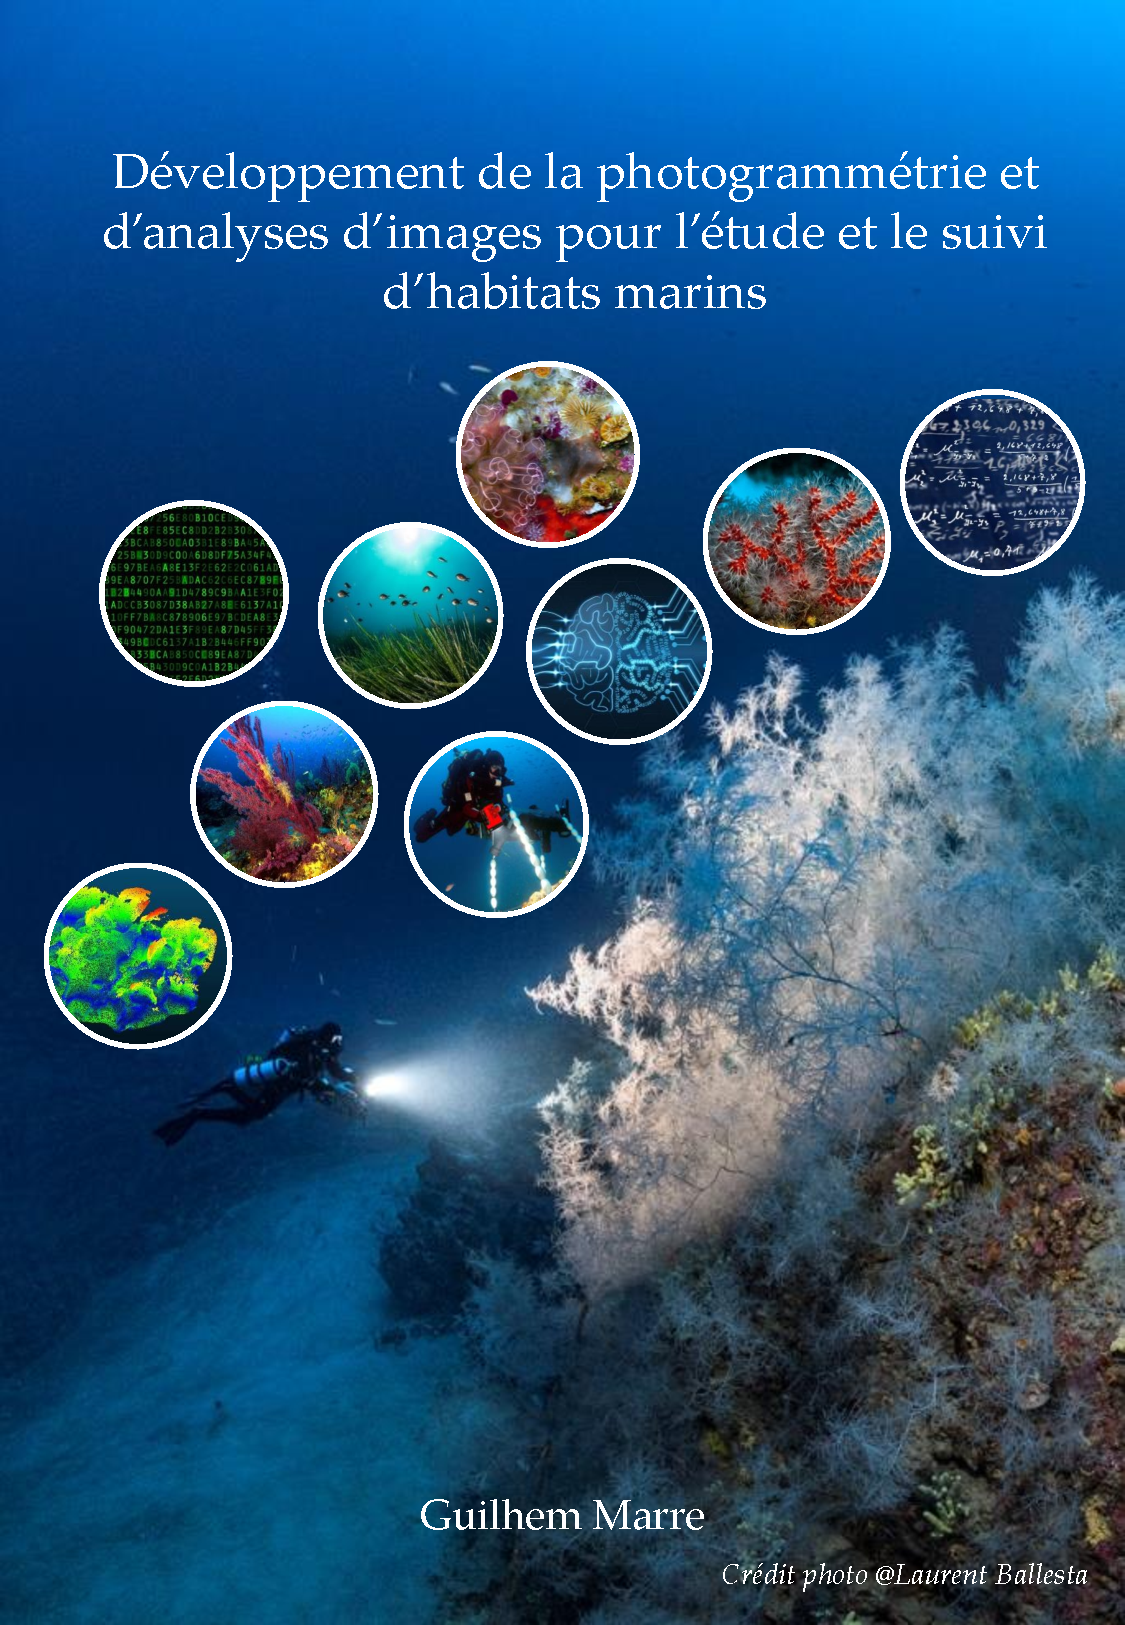
\includepdf[scale=1.02, pages=-,pagecommand={\thispagestyle{empty}}]{couverture_these_perso.pdf}

% Page blanche sans numérotation
\newpage
\clearpage
\thispagestyle{empty}
\hfill
\newpage

% Début numérotation chiffres romains
\pagenumbering{arabic} % roman

%%% Remerciements
\pagestyle{preambule}

\phantomsection
\addcontentsline{toc}{section}{REMERCIEMENTS}
{\centerline { {\sffamily \Large REMERCIEMENTS}}}

\vspace*{1cm}
\vskip 0.5cm
\noindent

J’ai toujours trouvé quelque peu ridicule la comparaison du rendu d’un manuscrit de thèse avec un accouchement, mais bien que la biologie ne me permette pas de faire l’expérience des deux, force est de constater qu’à seulement quelques heures de l'échéance, mes sentiments sont plutôt confus… Consécration d’un travail achevé ou frustration de ne pas avoir pu aller plus loin ? Joie de la libération et excitation de l’avenir ou nostalgie d’une période qui se termine et questionnements existentiels ? Quoiqu’il en soit, la thèse est décidément une expérience qui ne laisse pas indemne… Mais comme souvent, ce qui compte le plus ce sont les gens avec qui on partage ces moments importants…

« Je souhaite porter un toast ! »… mais par qui commencer ?

Tout d’abord, je tiens à remercier Florian, Pierre et Laurent, pour m’avoir accordé leur entière confiance dans la réalisation de ce travail de recherche. Sans votre soutien, je n’aurais probablement jamais fait de thèse, moi qui ne me destinais pas spécialement à la recherche et encore moins à l’épreuve du travail doctoral… J’ai commencé ma carrière andromedienne à remonter des bennes à sédiment, j’en ressors 4 ans plus tard avec une thèse, comme quoi tout est possible !

Bien sûr, je ne saurais que trop remercier mes chères et tendres directrices Julie et Sandra. Vous avez toujours été là pour moi, toujours de bons conseils, d’une efficacité redoutable et d’un optimisme inébranlable ! Tous les doctorants n’ont pas la chance d’avoir pareil encadrement, j’en suis bien conscient, et si ces trois années se sont si bien passées c’est en grande partie grâce à vous. 

Un grand merci également à vous tous qui avez enrichi ma réflexion scientifique et apporté un regard extérieur à mon travail. Je pense bien sûr aux membres de mon comité de thèse – Christiane Weber, Nicolas Mouquet, Gérard Subsol, François Guilhaumon et Maria Dornelas – pour votre bienveillance, votre disponibilité et vos précieux conseils, mais aussi à ceux qui m’ont accordé de leur temps pour parler deep learning – Dino Ienco, Jérôme Pasquet et Rémi Cresson – sans vous on ne serait pas allé aussi loin et aussi vite avec Cédric. En parlant du loup, un grand merci à Cédric De Almeida Braga qui a fait un super stage de M2. Ces quelques mois avec toi ont été un vrai plaisir, je te souhaite de te régaler dans ta thèse (à ton tour !) et dans ta vie rennaise.

Je souhaite bien évidemment remercier l’Agence de l’eau Rhône-Méditerranée-Corse pour son soutien financier et logistique dans ce projet de thèse et les réseaux de surveillance, sans quoi je n’aurais pas eu accès à autant de matière première pour mes recherches. Un grand merci à Pierre Boissery pour les échanges toujours riches d’enseignements, ses récits d'aventures et son regard pertinent concernant la gestion des habitats marins côtiers.

Comment écrire ses remerciements sans parler de ceux avec qui j’ai partagé mon quotidien au bureau ou en mer ? Un grand merci à tous les valeureux andromediens – Gwen, Marie, Anto, Sté, Agathe, Thomas, Seb, Célia, Caro et Sylvie – pour la bonne humeur au bureau et sur le terrain, vous êtes une deuxième famille! Et bien sûr merci aussi à tous les indep’ qu'on voit souvent – Thomas, Yaya, Nono, Mollon, Thibault, Justine, Mathieu… – pour avoir partagé avec vous tous ces moments de galère, de rires, ces belles plongées, ces couchers de soleil, ces mers démontées… J’ai énormément appris à vos côtés, techniquement et humainement, merci à vous !

Comme je suis chanceux, j’ai deux bureaux, donc deux fois plus de collègues ! Un grand merci à Florian et Marc pour ces deux ans et demi de cohabitation à la Maison de la Télédétection. C’était un plaisir de partager le bureau avec vous ! Il m’a semblé bien vide à votre départ… Merci Marc pour ton template LaTeX qui m'a permis de gagner beaucoup de temps et de m'y mettre sur le tard...  Mention spéciale aussi à mon cher Arthur pour être régulièrement monté nous voir pour discuter sciences et refaire le monde autour d’un café. Et bien sûr merci à tous les doctorants – Marc, Jacques, Christian, Eric, Dav, Hugo, Milo, Sarah, Fred… – pour l’ambiance agréable de travail et les pauses déjeuner au CIRAD. Enfin, merci à Isa pour l’accueil toujours aussi chaleureux dès l’arrivée à la MTD et à Baron pour les discussion socio-politiques !

Même s’il aura été une période compliquée pour tout le monde, y compris pour moi, je dois bien tirer mon chapeau au covid19 pour m’avoir permis d’avancer largement sur le travail de rédaction… Quoi de mieux qu’un confinement de deux mois pour finir de rédiger sa thèse ? Le timing semblait presque parfait… Merci !

Et bien sûr un grand merci à tous les copains qui sont une part plus qu’importante de ma vie. Merci à vous pour ces grosses soirées à l’Espantade, ces sessions kite, ces danses swing enflammées, ces festivals de fanfare, ces belles randos… merci pour cet oxygène que vous m’apportez au quotidien ! Un grand merci à toi ma Chonchon d’être toujours là pour moi, pour le meilleur comme pour le pire, depuis maintenant 12 ans ! Merci à mes fidèles colocataires de l’Espantade – Mimine, Alexia, Franz et Renan, mais aussi Thibaut, Claire, Mélo, Agathe… – de contribuer à ce bon vivre si spécial à notre belle maison. Merci aussi à toi papa pour ton aide toujours précieuse en bricolage, et merci à vous maman et Fannette d’être là dès que je vous sollicite pour un petit pépin de santé. Merci à vous trois d’être là, tout simplement. 

Ámbar, j’ai eu tant de plaisir à t’écouter chanter, sans imaginer une seule seconde qu’un jour nos chemins se croiseraient… Merci pour cette belle année passée à tes côtés, pour m'avoir supporté dans les deux sens du terme, tu es une personne magnifique et sensible. Je te souhaite de trouver le dosage entre musique et philosophie qui te rendra pleinement heureuse. Je suis fier de toi, et j'espère te revoir vite sur scène et en dehors.

Enfin, merci à ceux qui ont bien voulu relire ma thèse pour y déceler les dernières coquilles –  Renan, Gwen et Sylvie – et un grand merci aux deux valeureux rapporteurs qui ont accepté d’évaluer ce travail de thèse – Joaquim Garrabou et Thomas Corpetti – ainsi qu’aux autres membres du jury qui évalueront la soutenance – Stéphanie Manel, Sylvie Gobert et Sébastien Villéger. Merci à Laurent Ballesta pour les magnifiques photos qui permettent de donner un peu de couleur à ce manuscrit.

En vous souhaitant bonne lecture…


%Word cloud joli: https://wordart.com/create ou http://r-graph-gallery.com/
%With text mining to keep only keywords:
%http://www.sthda.com/english/wiki/text-mining-and-word-cloud-fundamentals-in-r-5-simple-steps-you-should-know#step-3-text-mining

\vskip 0.3cm
\noindent
 \qquad  \qquad \qquad \qquad \qquad \qquad \qquad \qquad \quad \textbf{Guilhem}


%%% Avant propos
\newpage
\begin{spacing}{1.5}
\phantomsection
\addcontentsline{toc}{section}{AVANT-PROPOS}
{\centerline { {\sffamily \Large AVANT-PROPOS}}}

\vspace*{1cm}
\vskip 0.5cm
\noindent

\normalsize
\noindent Cette thèse à été réalisée de septembre 2017 à juillet 2020 entre la société Andromède Océanologie (Carnon), l'UMR TETIS (INRAE, CIRAD, CNRS, AgroParisTech) et l'UMR MARBEC (Université de Montpellier, CNRS, IRD, Ifremer) à Montpellier. Ce travail a été cofinancé par Andromède Océanologie et l'Association Nationale de la Recherche et de la Technologie), et les missions de terrain ont principalement eu lieu dans le cadre des suivis environnementaux TEMPO (herbiers de posidonie) et RECOR (récifs coralligènes) financés par l'Agence de l'Eau Rhône-Méditerranée-Corse.

\medskip

\noindent Cette thèse a été dirigée par Julie Deter (UMR MARBEC) et Sandra Luque (UMRS TETIS), et a bénéficié des conseils avisés de Dino Ienco, Jérôme Pasquet et Rémi Cresson concernant les réseaux de neurones convolutifs, ainsi que des membres du comité de thèse Nicolas Mouquet, Gérard Subsol, François Guilhaumon, Maria Dornelas et Christiane Weber. 

\bigskip
\bigskip

%%% ARTICLES
\centerline{\textbf{\Large Publications}}

\medskip

% ARTICLE DEEP LEARNING
\noindent\href{https://doi.org/10.1016/j.ecoinf.2020.101110}{\textbf{Marre G.}, De Almeida Braga, C., Ienco, D., Luque, S., Holon, F., Deter, J. (2020). Deep convolutional neural networks to monitor coralligenous reefs: operationalizing biodiversity and ecological assessment. Ecological Informatics 59:101110}

\medskip

% ARTICLE METHODO
\noindent{\href{https://doi.org/10.3389/fmars.2019.00276}{\textbf{Marre, G.}, Holon, F., Luque, S., Boissey, P., Deter, J. (2019). Monitoring marine habitats with photogrammetry: a cost-effective, accurate, precise and high-resolution reconstruction method. Frontiers in Marine Science 6:276, 158–170}.}

\medskip

% ARTICLE HERBIERS
\noindent{\href{https://doi.org/10.3354/meps13338}{\textbf{Marre G.}, Deter, J., Holon, F., Boissery, P., Luque, S. (2020). Fine-scale automatic mapping of living \textit{Posidonia oceanica} seagrass beds with underwater photogrammetry. Marine Ecology Progress Series 643:63-74.}}

\bigskip
\bigskip

%%% AUTRES ARTICLES
\centerline{\textbf{\Large Autres publications}}

\noindent{\href{https://doi.org/10.3389/fmars.2019.00276}{Holon, F., \textbf{Marre, G.}, Parravicini, V., Mouquet, N., Bockel, T., Descamp, P., Tribot, A-S., Boissery, P., Deter, J. (2018). A predictive model based on multiple coastal anthropogenic pressures explains the degradation status of a marine ecosystem: Implications for management and conservation. Biological Conservation 222, 125-135.} Voir \autoref{annexe-holon}}

\clearpage
%%% RAPPORTS 
\centerline{\textbf{\Large Rapports d'activité}}

\noindent{\textbf{Marre, G.}, Holon, F., Delaruelle, G., Holon, F., Guilbert, A., Deter, J., 2017. Application de la photogrammétrie à la surveillance biologique: mise au point de la méthode. Rapport d'activité pour l'Agence de l'Eau Rhône-Méditerranée-Corse, 57 pages.}

\noindent{\textbf{Marre, G.}, Holon, F., Delaruelle, Fery, C., G., Holon, F., Guilbert, A., Deter, J., 2019. Acquisitions photogrammétriques 2018 - 2019 et développements méthodologiques. Rapport d'activité pour l'Agence de l'Eau Rhône-Méditerranée-Corse, 145 pages.}

\bigskip
\bigskip

%%% VULGARISATION
\centerline{\textbf{\Large Articles de vulgarisation scientifique}}

\noindent{\href{https://medtrix.fr/cahier-de-surveillance-3/}{\textbf{Marre, G.}, Luque, S., Holon, F., Boissery, P., Deter, J., 2018. Application de la photogrammétrie à la surveillance biologique des habitats sous-marins. Cahiers de la surveillance Medtrix n°3, Mars 2018.} Voir \autoref{annexe-cahiers}}

\medskip

\noindent{\href{https://www.agropolis.fr/publications/sciences-marines-et-littorales-en-occitanie-dossier-thematique-agropolis-international.php}{\textbf{Marre, G.}, Luque, S., Holon, F., Boissery, P., Deter, J., 2019. La photogrammétrie : une méthode d’observation innovante pour l’étude et la conservation du milieu marin. Les dossiers d'Agropolis International N°24: Sciences marines et littorales en Occitanie, Février 2019.}}

\bigskip
\bigskip

%%% PRESENTATIONS ORALES
\centerline{\textbf{\Large Communications dans des congrès}}

\noindent{\textbf{Marre, G.}, Ropars, B., 2017. At the crossroads between robotics, photogrammetry and ecology for the study of marine habitats. Communication orale au congrès Ecolotech. Salon de l'Ecologie, Montpellier, 9 novembre 2017.}

\medskip

\noindent{\textbf{Marre, G.}, Luque, S., Holon, F., Boissery, P., Deter, J., 2018. Rencontre entre robotique, photogrammétrie et écologie pour l'étude et le suivi des fonds marins. Communication orale au congrès Medtrix. Montpellier, 14 mars 2018. Voir \autoref{annexe-medtrix}}

\medskip

\noindent{\href{https://oreme.org/app/uploads/Oreme_AT16_G.Marre_.pdf}{\textbf{Marre, G.}, Luque, S., Holon, F., Boissery, P., Deter, J., 2018. Développement de la photogrammétrie pour 
l’étude et le suivi d’habitats marins. Communication orale à l'Apéro Technique de l'Observatoire des Sciences de l'Univers OREME. Montpellier, 28 mai 2018.}}

\medskip

\noindent{\textbf{Marre, G.}, Luque, S., Holon, F., Boissery, P., Deter, J., 2019. Méthodes photographiques pour la caractérisation de la structure et de la biodiversité des récifs coralligènes. Communication orale aux 10 ans de l'Observatoire des Sciences de l'Univers OREME. Montpellier, 11 octobre 2019.}

\medskip

\noindent{\textbf{Marre, G.}, Luque, S., Holon, F., Boissery, P., Deter, J., 2019. Suivi de communautés coralligènes par des
réseaux de neurones convolutifs. Communication orale au congrès Ecolotech. Salon de l'Ecologie, Montpellier, 7 novembre 2019.}

\medskip

\noindent{\textbf{Marre, G.}, Luque, S., Holon, F., Boissery, P., Deter, J., 2019. Photogrammétrie sous-marine et analyses d’images pour le suivi d’habitats benthiques Méditerranéens. Communication orale acceptée au congrès Merigeo à Bordeaux en mars 2020. Reporté à cause du Covid-19 à Nantes, novembre 2020. Voir \autoref{annexe-merigeo}}

\bigskip
\bigskip

%%% ENCADREMENT
\centerline{\textbf{\Large Activités d'encadrement}}

\noindent{Co-encadrement du stage de fin d'études (M2 - cursus ingénieur) de \textbf{Gaïlé Lejay} en 2018, ayant donné lieu à la rédaction d'un mémoire de fin d'études : "Utilisation de modèles 3D en écologie sous-marine, détermination d’indicateurs dérivés des modèles et analyse de la variation des paramètres selon l’état de conservation des habitats".}

\medskip

\noindent{Co-encadrement du stage de fin d'études (M2 - Computer Science) de \textbf{Cédric De Almeida Braga} en 2019, ayant donné lieu à la rédaction d'un mémoire de fin d'études : "Characterization of coralligenous assemblages : from automatic image classification to 3D species mapping".}


\bigskip
\bigskip

%%% FORMATIONS
\centerline{\textbf{\Large Formations suivies}}

\noindent{\textbf{Plongée recycleur Inspiration} - Carnon - Novembre 2017 (5 jours)}

\medskip

\noindent{\textbf{Python 3 : des fondamentaux aux concepts avancés du langage} - MOOC - Janvier 2018 (25 heures)}

\medskip

\noindent{\textbf{Linux pour les sciences} - Montpellier - Septembre 2018 (6 heures)}

\medskip

\noindent{\textbf{Data Sciences for Geosciences} - Brest - Janvier 2019 (5 jours)}

\medskip

\noindent{\textbf{Ethique de la recherche} - MOOC - Novembre 2019 (15 heures)}

\medskip

\noindent{\textbf{Plongée recycleur trimix hypoxique} - La Ciotat - Décembre 2019 (5 jours)}

\medskip




\bigskip
\bigskip

\newpage
%%% CAMPAGNES DE TERRAIN
\centerline{\textbf{\Large Campagnes de terrain}}

\noindent{\textbf{Réseaux de surveillance TEMPO / RECOR} - Corse - Juin 2017 (14 jours)}

\medskip

\noindent{\textbf{Suivi de transplantation de l'herbier du Larvotto} - Monaco - Juin - Juillet 2017 (10 jours)}

\medskip

\noindent{\textbf{Suivi du récif coralligène des Spélugues} - Monaco - Aout 2017 (4 jours)}

\medskip

\noindent{\textbf{Expériences premier article} - Roquebrune - Novembre 2017 (2 jours)}

\medskip

\noindent{\textbf{Suivi du récif coralligène des Spélugues} - Monaco - Janvier 2018 (5 jours)}

\medskip

\noindent{\textbf{Suivi de transplantation de l'herbier du Larvotto} - Monaco - Février 2018 (4 jours)}

\medskip

\noindent{\textbf{Suivi du récif coralligène des Spélugues} - Monaco - Avril 2018 (4 jours)}

\medskip

\noindent{\textbf{Réseaux de surveillance TEMPO / RECOR} - Occitanie - Juin 2018 (8 jours)}

\medskip

\noindent{\textbf{Restauration d'un récif coralligène (RESCOR)} - Saint-Jean-Cap-Ferrat - Octobre 2018 (3 jours)}

\medskip

\noindent{\textbf{Suivis des récifs artificiels de Cortiou (REXCOR)} - Marseille - Octobre 2018 (2 jours)}

\medskip

\noindent{\textbf{Cartographie en plongée tractée (CartoTract)} - Golfe Juan / Cannes - Septembre 2018 (2 jours)}

\medskip

\noindent{\textbf{Mise au point de l'acquisition acoustique et photogrammétrie (GOMBESSA)} - Villefranche-sur-Mer - Mars 2019 (2 jours)}

\medskip

\noindent{\textbf{Restauration d'un récif coralligène (RESCOR)} - Saint-Jean-Cap-Ferrat - Avril 2019 (5 jours)}

\medskip

\noindent{\textbf{Réalisation d'images complémentaires pour le tournage de GOMBESSA V} - Capraia, Italie - Avril 2019 (5 jours)}

\medskip

\noindent{\textbf{Suivis des rejets de station d'épuration} - Agglomération de Marseille - juin 2019 (3 jours)}

\medskip

\noindent{\textbf{Réseaux de surveillance TEMPO / RECOR} - PACA - Juin 2019 (4 jours)}

\medskip

\noindent{\textbf{Suivis des récifs artificiels de Cortiou (REXCOR)} - Marseille - Juin 2019 (2 jours)}

\medskip

\noindent{\textbf{Suivis des récifs artificiels de Cortiou (REXCOR)} - Marseille - Septembre 2019 (2 jours)}

\medskip

\noindent{\textbf{Réseaux de surveillance TEMPO / RECOR} - Occitanie - Mai 2020 (3 jours)}

\medskip

\noindent{\textbf{Réseaux de surveillance TEMPO / RECOR} - Corse - Mai 2020 (24 jours)}

\medskip

\end{spacing}

% chiffres clés de la thèse
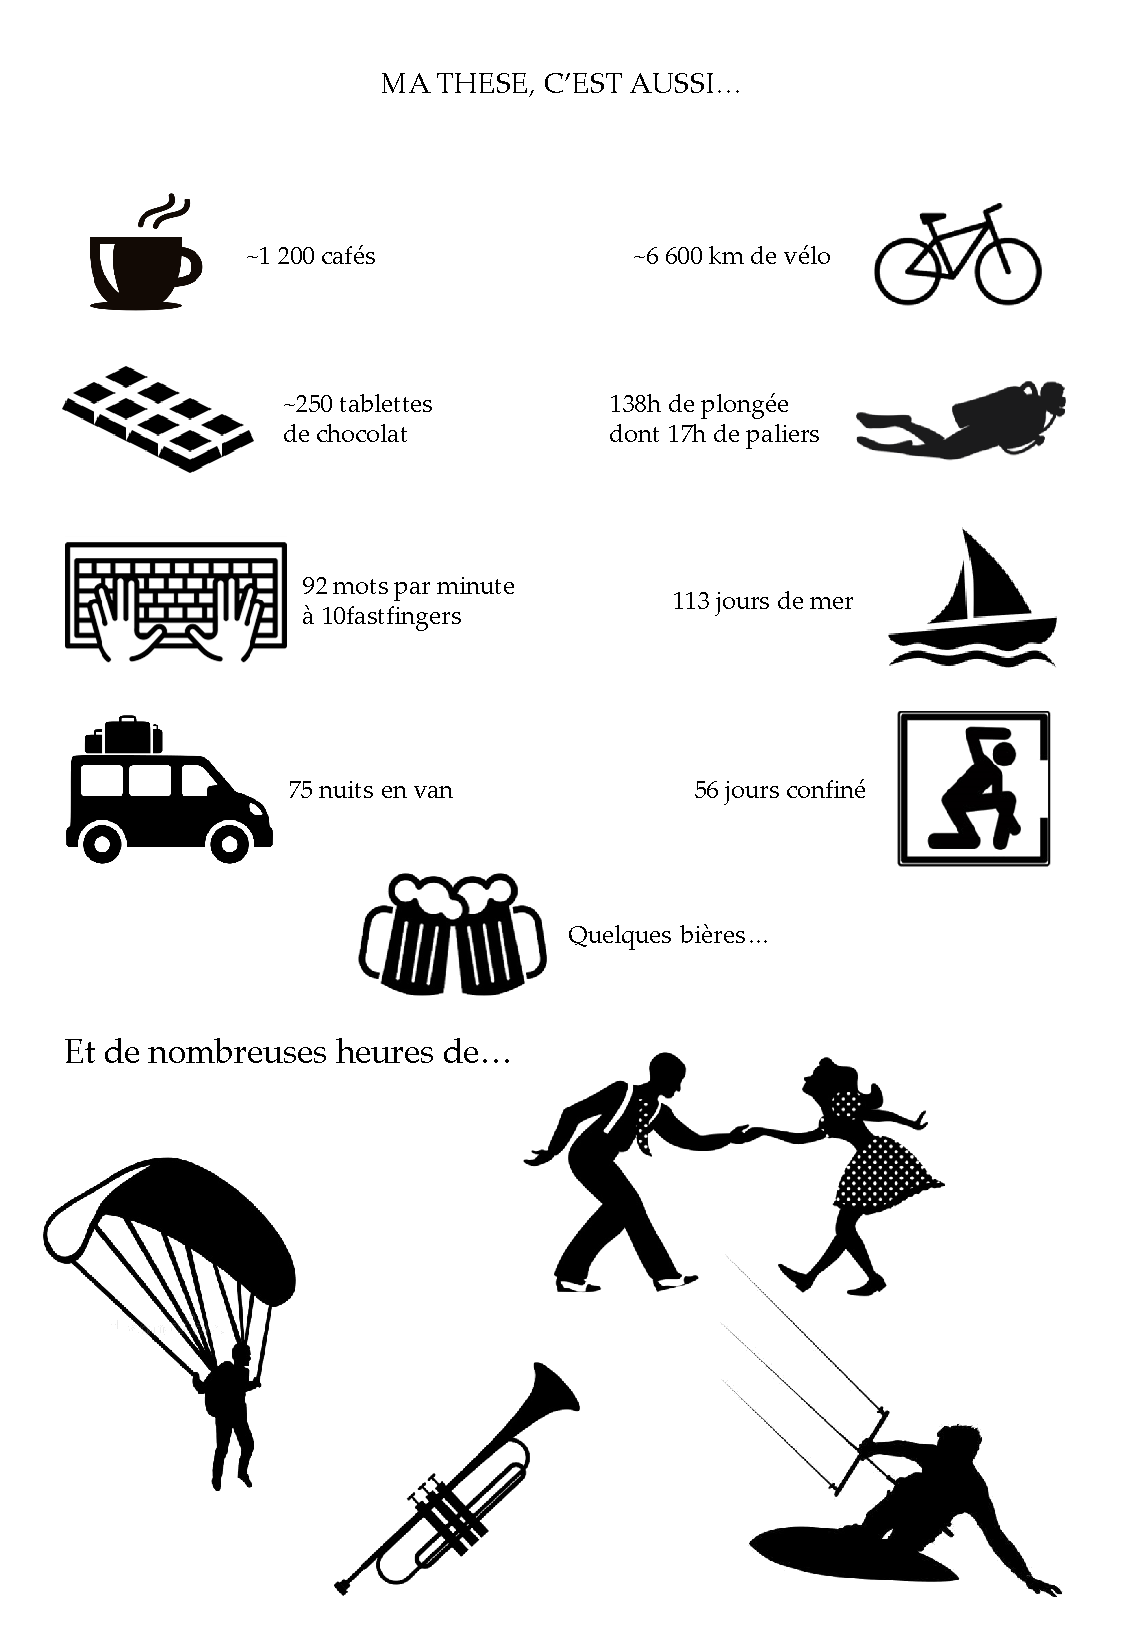
\includepdf[scale=0.85, pages=-,pagecommand={\thispagestyle{preambule}}]{./images/chiffres_cles.pdf}

%%% Table des matières
\newpage
\begingroup
\hypersetup{linkcolor=black}
%\begin{spacing}{1.5}
% \advance\cftchapnumwidth -0.5em\relax % tentative de réduire l'espace entre numéro de chapitre et nom dans la toc...
	\tableofcontents
%\end{spacing}
\endgroup
\newpage

%%% Liste des figures
\newpage
%For Removing Extra Space in List of Tables and Figures before every chapter
\let\origaddvspace\addvspace % on stock addvspace dans origaddvspace
\renewcommand{\addvspace}[1]{}
\begingroup
\hypersetup{linkcolor=black}
\begin{spacing}{1.5}
	\phantomsection
	\addcontentsline{toc}{section}{LISTE DES FIGURES}
	\setcounter{lofdepth}{2} \listoffigures
\end{spacing}
\endgroup
\newpage

%%% Liste des tableaux
\newpage
\begingroup
\hypersetup{linkcolor=black}
\begin{spacing}{1.5}
	\phantomsection
	\addcontentsline{toc}{section}{LISTE DES TABLEAUX}
	\setcounter{lotdepth}{2} \listoftables
\end{spacing}
\endgroup
\newpage


% Restauration de la valeur originale de addvspace
\renewcommand{\addvspace}[1]{\origaddvspace{#1}}

% Page blanche sans numérotation
\newpage
\clearpage
\thispagestyle{empty}
\hfill
\newpage

%\mainmatter % partie principale du bouquin % Sinon la numérotation redémarre de là
\pagestyle{main}
%\pagenumbering{arabic} % On commence la numérotation en chiffres arabes


%%% Introduction
\part{Introduction générale}
\pagestyle{preambule}
%\chapter{Introduction générale} \label{Introduction générale}

% COVER PAGE
\centerline{\bfseries\textcolor{bleusection}{ \Huge Introduction générale}}  

\bigskip

% Figure cover
\begin{tikzpicture}
  \def\ig{%
   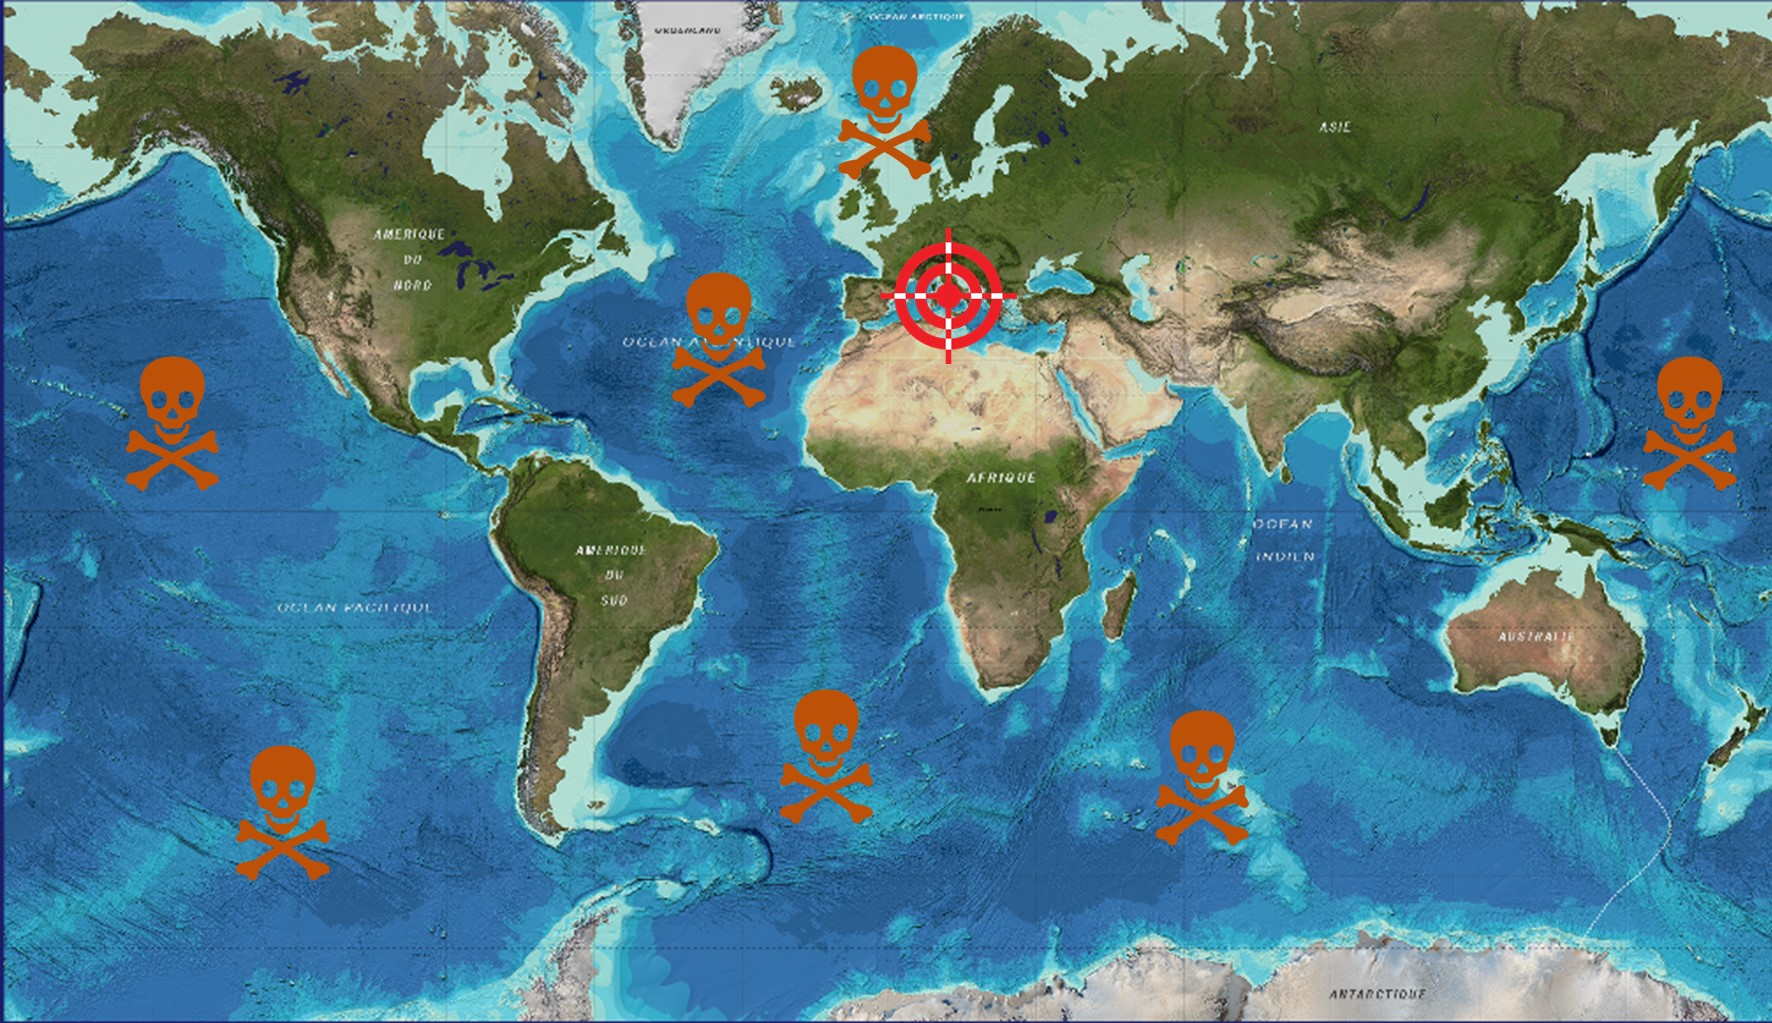
\includegraphics[width=\linewidth,keepaspectratio]{./1_intro/cover_intro}}
 \node [inner sep=0pt](mypicture) at (0,0) {\phantom{\ig}};
 \clip[rounded corners=5mm] ($(mypicture.south west)+(\bord,\bord)$) rectangle ($(mypicture.north east)-(\bord,\bord)$);
 \node[inner sep=0pt](mypicture) at (0,0) {\ig};
\end{tikzpicture}


% Table des matières intro
{\LARGE
\begin{enumerate}[label=\textcolor{bleusection}{\arabic*}{.}, leftmargin=2cm]
  \item \nameref{intro.1}
  \item \nameref{intro.2}
  \item \nameref{intro.3}
\end{enumerate}
}

% DEBUT INTRO
\clearpage
\pagestyle{intro}


\section{Une biodiversité marine en danger}\label{intro.1}

\subsection{Distribution de la biodiversité marine mondiale}\label{intro.1.1}

Les océans couvrent plus de 70 \% de la surface de la Terre, abritent 50 à 80 \% des espèces vivantes de notre planète \citep{mora_how_2011, costello_global_2013}, et génèrent plus de 60 \% des services écosystémiques mondiaux \citep{millenium_ecosystem_assessment_ecosystem_2005, bindoff_changing_2019, ipbes_global_2019}, dont la moitié de la production du dioxygène atmosphérique par photosynthèse. L’océan global est un organe clé de la régulation du système climatique, via les flux thermiques et biogéochimiques qu’il entretient avec l’atmosphère ; il est notamment responsable de l’absorption de plus de 25 \% des émissions annuelles de CO\textsubscript{2} d’origine anthropique \citep{heinze_ocean_2015}.

L’étendue géographique de l’océan global, du pôle Sud au pôle Nord, ainsi que sa très forte anisotropie verticale (notamment température et lumière) créent de nombreuses niches écologiques, peu à peu exploitées au cours de l’évolution par une grande diversité de formes vivantes. Si la répartition de la biodiversité océanique mondiale dépend du taxon considéré, elle est plus importante en milieu côtier \citep{tittensor_global_2010}, et particulièrement forte en milieu tropical, notamment dans le « triangle de corail » \citep{sanciangco_habitat_2013} (Malaisie, Indonésie, Philippines et îles Salomon ; \autoref{figure_intro1}).

%%%%%%%%%%%%%%%%%%%%%%%%%%%%%%%%%%%%%%%%%%%%%%%%%%%%%%%%%%%%%
%%% Figure intro1: Cartographie de la richesse spécifique %%%
%%%%%%%%%%%%%%%%%%%%%%%%%%%%%%%%%%%%%%%%%%%%%%%%%%%%%%%%%%%%%
\begin{figure}[H]
	\begin{center}
	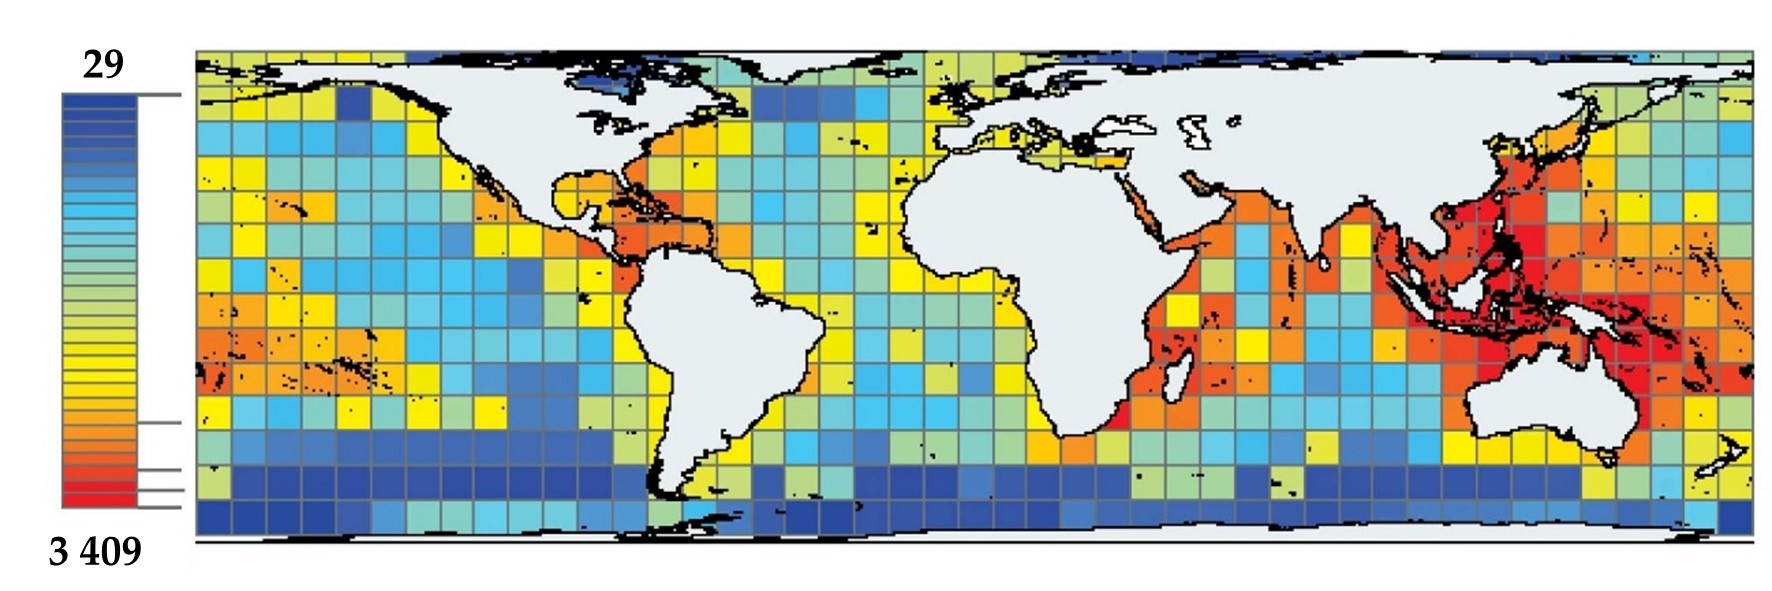
\includegraphics[width=\linewidth,keepaspectratio]{./1_intro/global_diversity_Tittensor2010}
		\caption[Cartographie de la richesse spécifique mondiale tous taxa confondus]{Cartographie de la richesse spécifique mondiale tous taxa confondus (d'après \citet{tittensor_global_2010}). Données compilées pour 11 567 espèces appartenant à 13 taxa différents.}
	\label{figure_intro1}
\end{center}
\end{figure}

\subsection{Une biodiversité sous pression}\label{intro.1.2}

\subsubsection{Contexte de changement global}\label{intro.1.2.1}
La compréhension de la distribution des espèces ainsi que des forces structurant les assemblages ont toujours intéressé les biologistes depuis les premiers travaux de Darwin \citep{darwin_origin_1859}. La prise en compte des impacts anthropiques sur la biodiversité mondiale et l’urgence de mettre en place des plans de conservation efficaces pour sa préservation \citep{margules_systematic_2000} ont motivé la poursuite des études sur les patrons de biodiversité à différentes échelles spatiales \citep{rosa_multiscale_2017}. En effet, la très forte intensification des émissions de gaz à effet de serre depuis le début de l’ère industrielle a déjà contribué à d’importantes perturbations du système climatique à toutes les échelles spatiales, et les projections indiquent une poursuite de ces modifications climatiques pour les décennies à venir \citep{ipcc_climate_2013}. Cette altération du climat, associée aux autres pressions anthropiques (déforestation, surpêche, pollutions chimiques…), a déjà largement affecté la biosphère au point d’initier la « sixième crise d’extinction d’espèces » \citep{barnosky_has_2011, dirzo_defaunation_2014, ceballos_accelerated_2015}. Tous les scénarii indiquent que cette érosion de la biodiversité devrait se poursuivre au cours du 21e siècle \citep{pereira_scenarios_2010, tittensor_mid-term_2014, visconti_projecting_2016}.

Les océans ne sont pas indemnes des impacts de « l’Anthropocène » \citep{mcgill_fifteen_2015}, et l’érosion de la biodiversité marine continue de s’accélérer \citep{mccauley_marine_2015, bindoff_changing_2019, ohara_mapping_2019}. En effet, la température est le principal facteur environnemental régissant la distribution des espèces marines \citep{tittensor_global_2010}, et les modifications de la température des océans questionnent sur une possible redistribution des espèces et des assemblages écologiques à l’échelle globale \citep{pereira_scenarios_2010, tittensor_global_2010, poloczanska_responses_2016}. Les habitats marins côtiers sont particulièrement vulnérables dans la mesure où ils abritent une importante biodiversité \citep{halpern_global_2008} et sont directement soumis à une population humaine beaucoup plus dense que la moyenne (27 \% de la population mondiale vit à moins de 100 km de la côte \citep{kummu_over_2016}). Parmi eux, les récifs coralliens sont largement étudiés, car ils contiennent à eux seuls environ 35 \% de la biodiversité marine mondiale \citep{reaka-kudla_biodiversity_2005} et sont largement touchés par le changement climatique \citep{hoegh-guldberg_coral_2007, death_27-year_2012, graham_predicting_2015, hughes_coral_2017}. Bien que certains assemblages tempérés semblent plus robustes que les récifs coralliens tropicaux aux changements globaux \citep{stuart-smith_stability_2010}, la majorité des biomes marins sont susceptibles d’être affectés \citep{waycott_accelerating_2009, marba_mediterranean_2014, telesca_seagrass_2015, wernberg_climate-driven_2016, halpern_recent_2019, ohara_mapping_2019}. Les résultats plus mitigés en milieu tempéré pourraient être en partie expliqués par un manque de données pour ces habitats \citep{wernberg_impacts_2011}. En effet, la situation en 2008 indiquait que plus de 40 \% des océans subissaient déjà un fort impact anthropique cumulé \citep{halpern_global_2008}, et cet impact a significativement augmenté au cours de la dernière décennie pour près de 60 \% des océans \citep{halpern_recent_2019} (\autoref{figure_intro2}). Aujourd’hui, près de la totalité de l’océan mondial (97,7 \%) est affectée par plusieurs pressions anthropiques \citep{halpern_spatial_2015} et 83 \% de l’océan global abrite plus de 25 \% d’espèces menacées \citep{ohara_mapping_2019}.

%%%%%%%%%%%%%%%%%%%%%%%%%%%%%%%%%%%%%%%%%%%%%%%%%%%
%%% Figure intro2: Cartographie impacts cumulés %%%
%%%%%%%%%%%%%%%%%%%%%%%%%%%%%%%%%%%%%%%%%%%%%%%%%%%
\begin{figure}[H]
	\begin{center}
	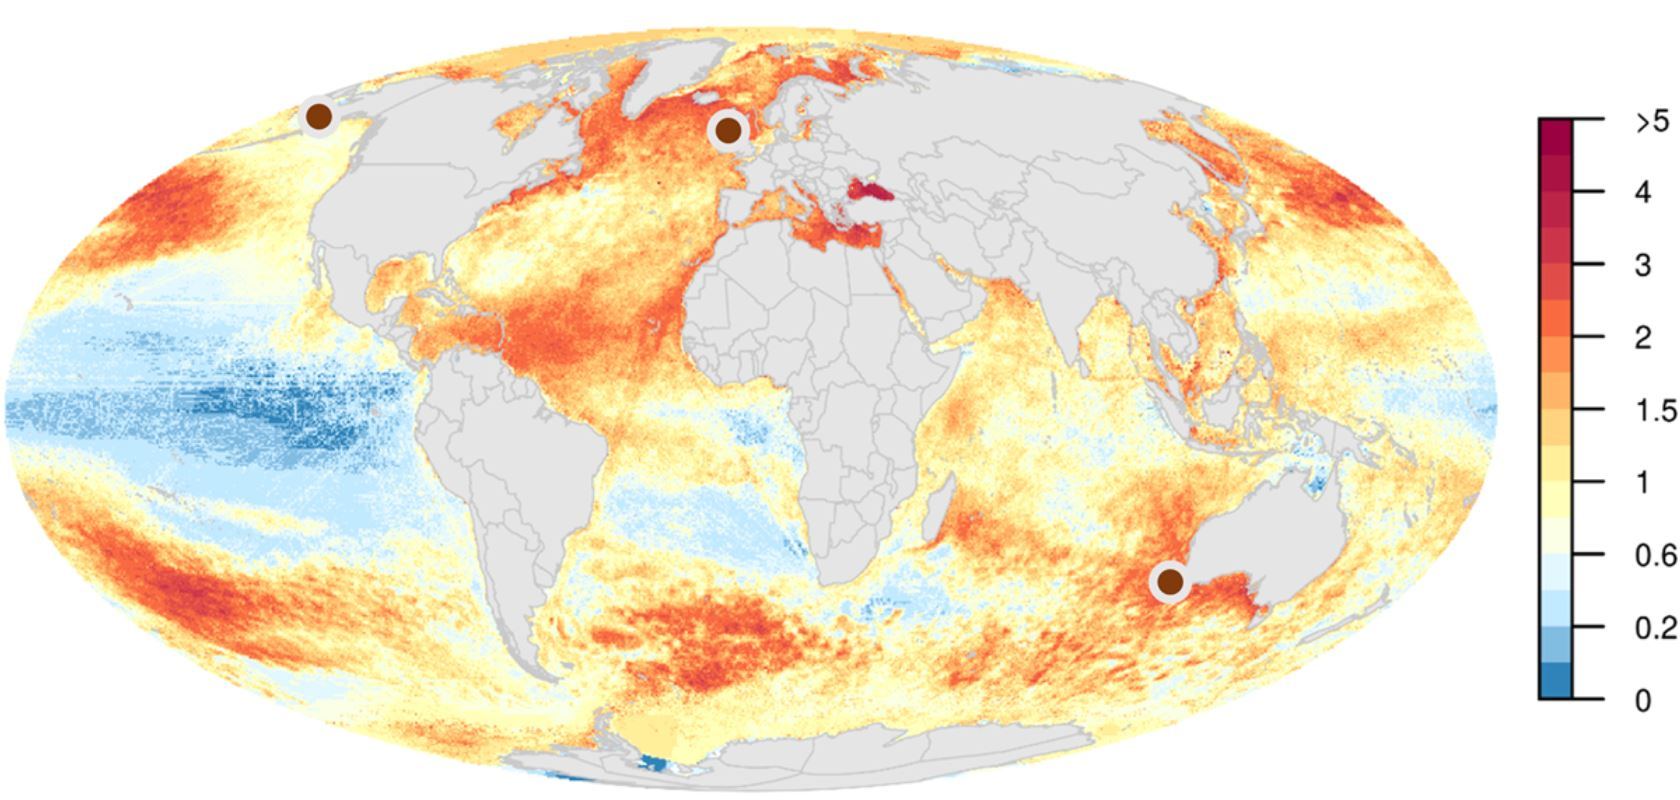
\includegraphics[width=\linewidth,keepaspectratio]{./1_intro/cumulative_impacts_Halpern2019}
		\caption[Cartographie des impacts anthropiques cumulés à l’échelle mondiale]{Cartographie des impacts anthropiques cumulés à l’échelle mondiale (d'après \citet{halpern_recent_2019}).}
	\label{figure_intro2}
\end{center}
\end{figure}

\subsubsection{Pressions anthropiques locales}\label{intro.1.2.2}
Les changements globaux induits par les émissions massives de gaz à effet de serre depuis le début de l’ère industrielle ne sont malheureusement pas les seuls facteurs affectant la biodiversité, et les écosystèmes sont menacés à l’échelle globale par de multiples pressions anthropiques \citep{hoekstra_confronting_2004, halpern_global_2008}. Par exemple, la fragmentation et la perte d’habitats ont des effets considérables sur leur biodiversité \citep{brooks_habitat_2002, haddad_habitat_2015}. Les habitats marins, bien qu’en apparence protégés de l’action de l’Homme, subissent d’importantes pressions anthropiques locales \citep{micheli_cumulative_2013, halpern_spatial_2015, holon_predictive_2018} (\autoref{figure_intro3}), avec notamment : \textbf{la pêche} (dégradation des habitats par chalutage \citep{hiddink_global_2017}, effondrement des stocks halieutiques à cause de la surpêche \citep{christensen_century_2014, essington_fishing_2015, link_global_2019} et impacts des engins de pêche laissés à l’abandon \citep{wilcox_understanding_2015, moschino_is_2019}), \textbf{les aménagements côtiers} (destruction des habitats et perturbation des régimes hydrosédimentaires favorisant la sédimentation sur des habitats sensibles \citep{airoldi_effects_2003, holon_predictive_2018}), \textbf{les pratiques agricoles} (enrichissement en nitrates et phosphates modifiant la structure des communautés \citep{berger_effects_2003, savage_effects_2010}), \textbf{les rejets de station d’épuration} (pathogènes, matière organique et nutriments altèrent la qualité de l’eau et affectent les habitats limitrophes \citep{orth_global_2006, waycott_accelerating_2009}), \textbf{le trafic maritime} (collisions avec les cétacés \citep{peltier_monitoring_2019}, perturbation des vertébrés marins \citep{bruintjes_rapid_2016, simpson_anthropogenic_2016, bas_marine_2017,slabbekoorn_effects_2018}), \textbf{le mouillage} (dégradation des herbiers sous-marins \citep{short_natural_1996} et des récifs biogéniques \citep{ballesteros_mediterranean_2006} par l’action mécanique de l’ancre et de la chaîne \citep{milazzo_boat_2004}), \textbf{les espèces exotiques envahissantes} (une des principales causes d’extinction d’espèces \citep{bellard_alien_2016}, considérée comme l’un des plus grands défis en matière de conservation \citep{pysek_invasive_2010}), et \textbf{les rejets de macro-déchets plastiques} (chaque année, plus de 300 millions de tonnes de déchets plastiques atterrissent dans l’océan global \citep{law_plastics_2017} et contaminent un nombre significatif d’espèces marines les ingérant \citep{schuyler_global_2013, wilcox_threat_2015}).

%%%%%%%%%%%%%%%%%%%%%%%%%%%%%%%%%%%%%%%%%%%%%%%%%%%%%%%%%%
%%% Figure intro3: Illustration pressions anthropiques %%%
%%%%%%%%%%%%%%%%%%%%%%%%%%%%%%%%%%%%%%%%%%%%%%%%%%%%%%%%%%
\begin{figure}[H]
	\begin{center}
	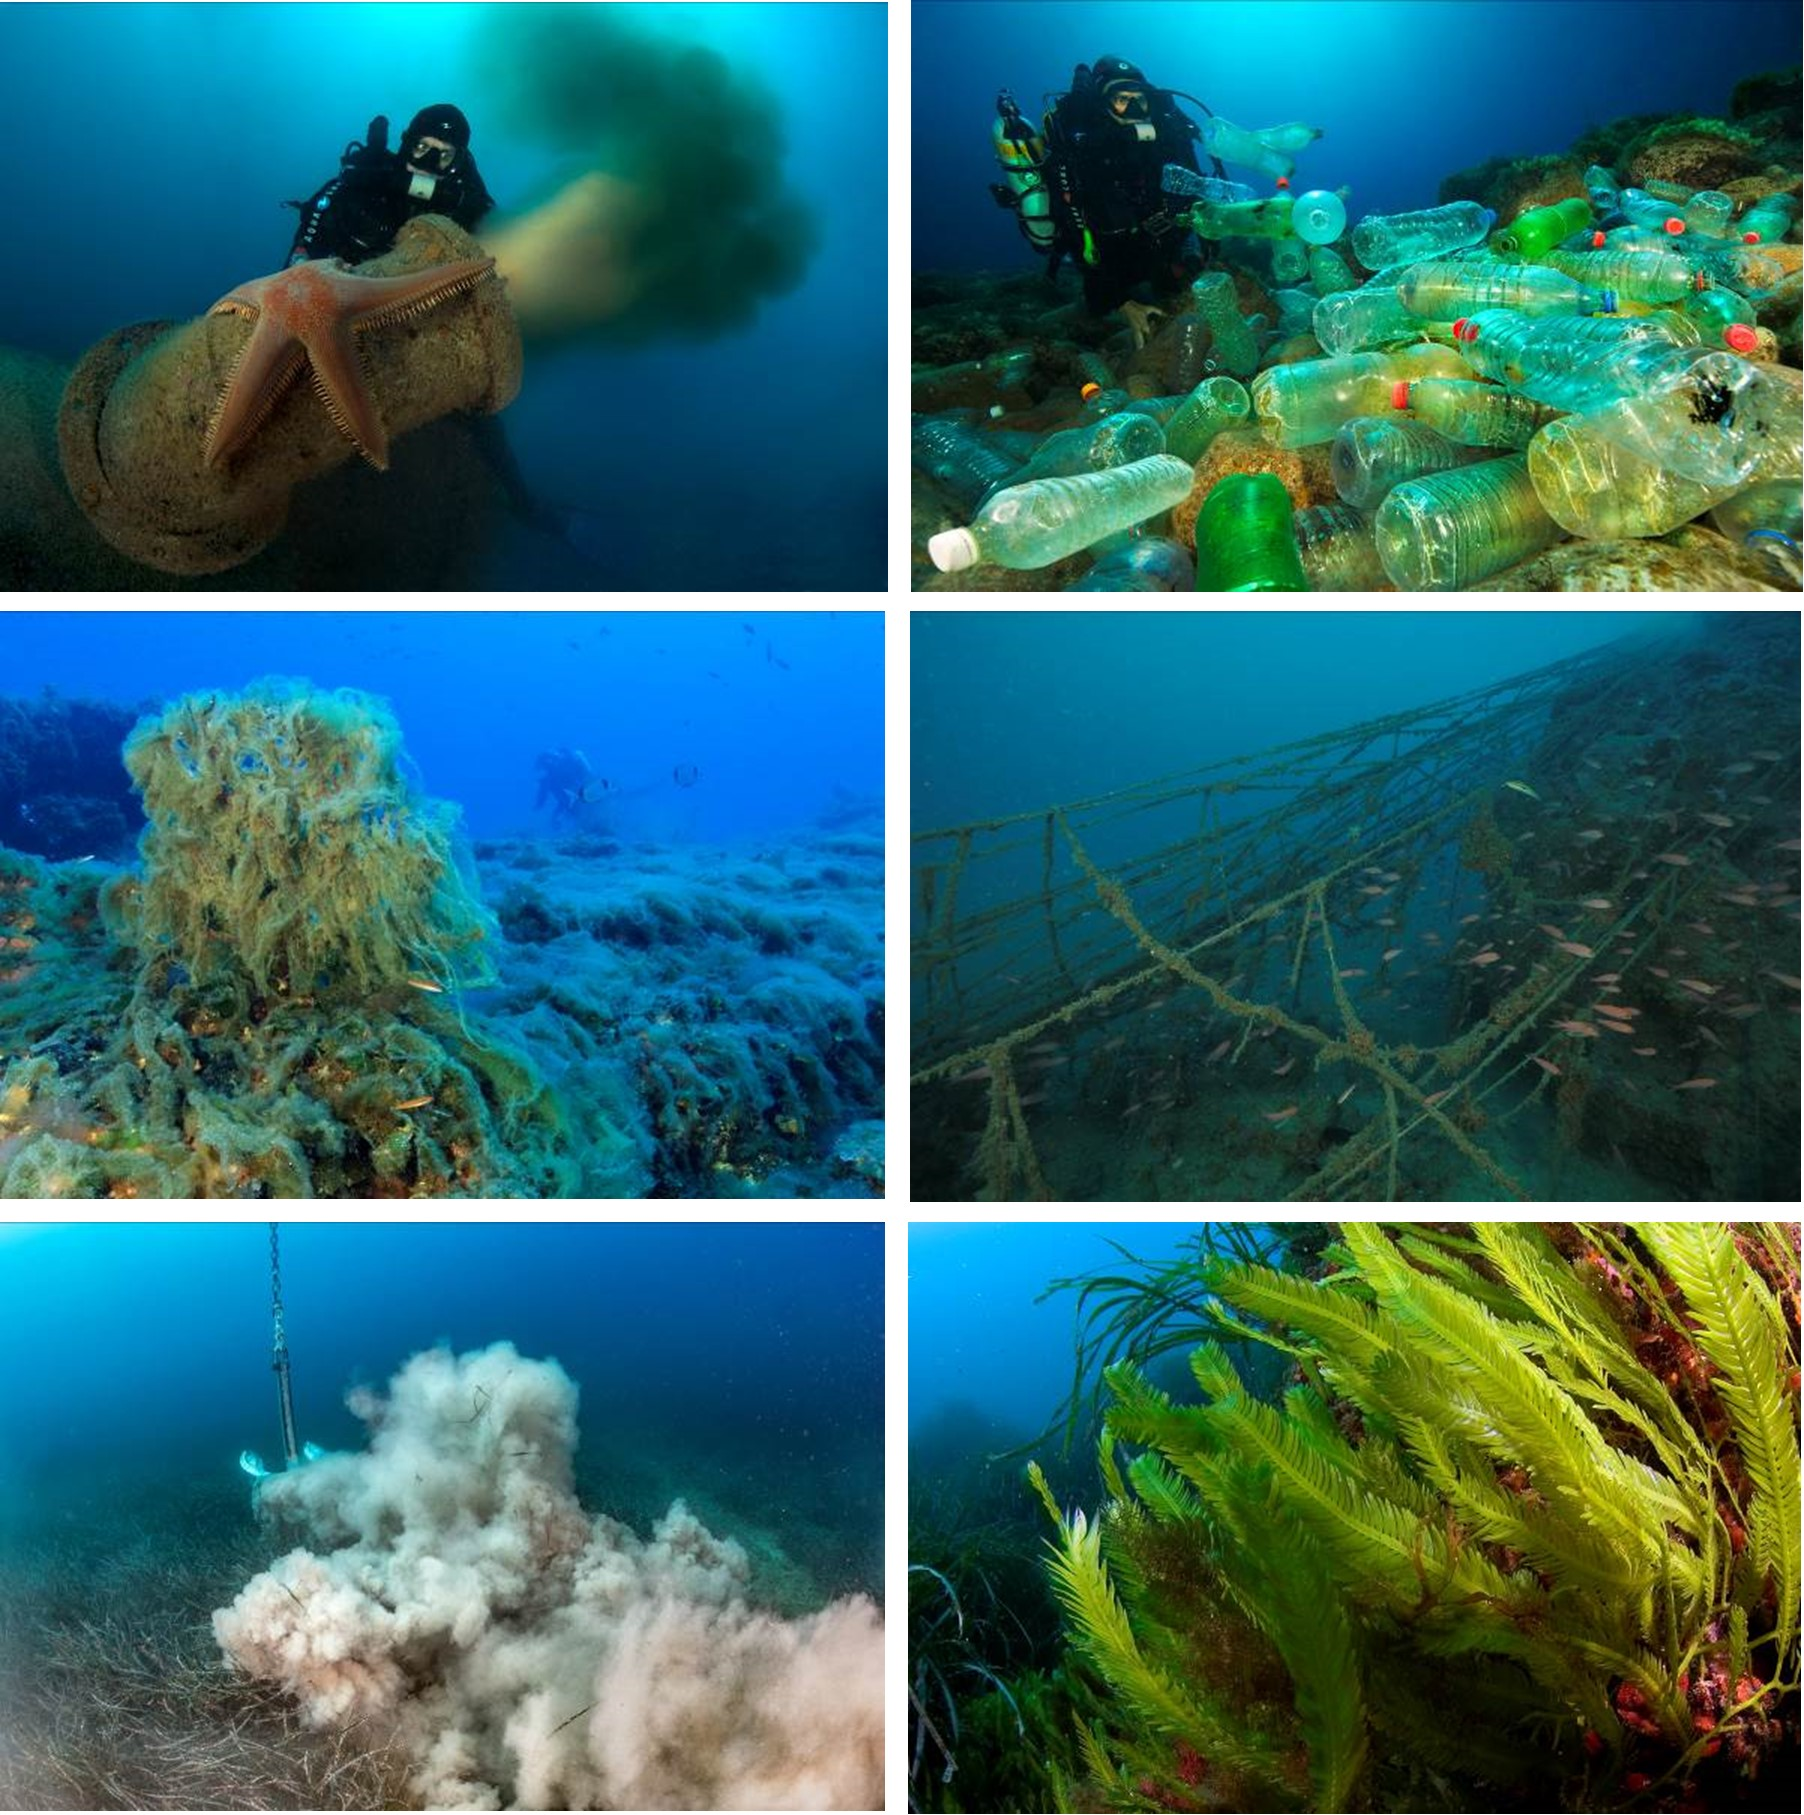
\includegraphics[width=\linewidth,keepaspectratio]{./1_intro/pressions}
		\caption[Illustrations de quelques pressions anthropiques]{Illustrations de quelques pressions anthropiques. De gauche à droite et de haut en bas: rejet de station d’épuration, macro-déchets plastiques, algues filamenteuses recouvrant un récif coralligène et ses gorgones, ancien engin de pêche coincé sur un récif coralligène, relève d’une ancre d’un bateau au mouillage dans l’herbier, présence d’une espèce exotique envahissante (\textit{Caulerpa taxifolia}) dans un herbier de posidonie (\textit{©Andromède Océanologie}).}
	\label{figure_intro3}
\end{center}
\end{figure}

\subsection[La Méditerranée: une exceptionelle biodiversité soumise à d’importantes pressions]{La Méditerranée: une exceptionelle biodiversité soumise à \\ d’importantes pressions}\label{intro.1.3}

Située entre l’Europe et l’Afrique, la mer Méditerranée est ce qu’il reste aujourd’hui de l’océan Téthys. Son histoire géologique intense, sa géomorphologie et ses conditions environnementales ont largement contribué à son histoire évolutive et à l’exceptionnelle biodiversité qui la caractérise depuis la fin de l’Éocène (-42 Ma à -39 Ma) \citep{boudouresque_marine_2004, renema_hopping_2008}. Aujourd’hui, alors qu’elle ne représente que 0,32 \% du volume de l’océan global, la mer Méditerranée abrite près de 7 \% de la biodiversité marine mondiale (17 000 espèces) \citep{coll_biodiversity_2010} dont environ un quart est endémique au bassin \citep{bianchi_rmesualtrsine_2000}. L’essentiel de cette biodiversité se concentre sur le plateau continental, notamment les poissons et les invertébrés benthiques (vivant sur le fond) \citep{coll_mediterranean_2012, katsanevakis_invading_2014} (\autoref{figure_intro4}). L’exploitation des ressources halieutiques a été un facteur primordial dans l’établissement et le développement des civilisations autour du bassin Méditerranéen au cours de l’histoire \citep{coll_biodiversity_2010}, mais représente aujourd’hui une menace pour cette biodiversité côtière. Par ailleurs, la Méditerranée n’est pas épargnée par les changements climatiques et représente une des régions les plus vulnérables aux perturbations climatiques futures \citep{giorgi_climate_2006, adloff_mediterranean_2015}. Les herbiers de posidonie (Posidonia oceanica) et les récifs coralligènes, qui figurent parmi les habitats marins les plus riches de Méditerranée \citep{boudouresque_marine_2004}, sont particulièrement sujets aux fortes pressions anthropiques globales et locales. 

%%%%%%%%%%%%%%%%%%%%%%%%%%%%%%%%%%%%%%%%%%%%%%%%%%%%%%%
%%% Figure intro4: Richesse spécifique Méditerranée %%%
%%%%%%%%%%%%%%%%%%%%%%%%%%%%%%%%%%%%%%%%%%%%%%%%%%%%%%%
\begin{figure}[H]
	\begin{center}
	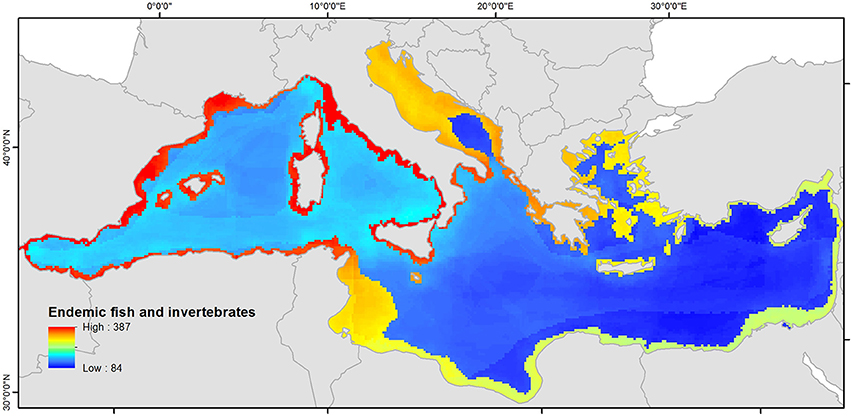
\includegraphics[width=\linewidth,keepaspectratio]{./1_intro/species_richness_Katsanevakis2014}
		\caption[Richesse spécifique des poissons et invertébrés endémiques en Méditerranée]{Richesse spécifique des poissons et invertébrés endémiques en Méditerranée \citep{katsanevakis_invading_2014}.}
	\label{figure_intro4}
\end{center}
\end{figure}

\subsubsection{Les herbiers de Posidonie : un habitat fragile aux multiples services écosystémiques}\label{intro.1.3.1}

La notion de services écosystémiques vise à quantifier l’ensemble des bénéfices que les humains tirent du fonctionnement et de l’intégrité des écosystèmes \citep{de_groot_global_2012}. Si les services attribués aux écosystèmes marins sont encore peu documentés \citep{townsend_challenge_2018}, plus de la moitié de la valeur du capital naturel et des services écosystémiques mondiaux sont attribués aux seuls herbiers sous-marins \citep{millenium_ecosystem_assessment_ecosystem_2005, ipbes_global_2019}. En effet, leurs rôles écologiques et économiques sont cruciaux : séquestration de carbone dans les rhizomes et la matte, production primaire locale pour les herbivores, export de matière organique vers les habitats à faible production, oxygénation de la colonne d’eau, atténuation de la houle, fixation du sédiment et des matières en suspension, nurserie à poissons… (\autoref{figure_intro5}).

%%%%%%%%%%%%%%%%%%%%%%%%%%%%%%%%%%%%%%%%%%%%%%%%%%%%%%%
%%% Figure intro5: Richesse spécifique Méditerranée %%%
%%%%%%%%%%%%%%%%%%%%%%%%%%%%%%%%%%%%%%%%%%%%%%%%%%%%%%%
\begin{figure}[H]
	\begin{center}
	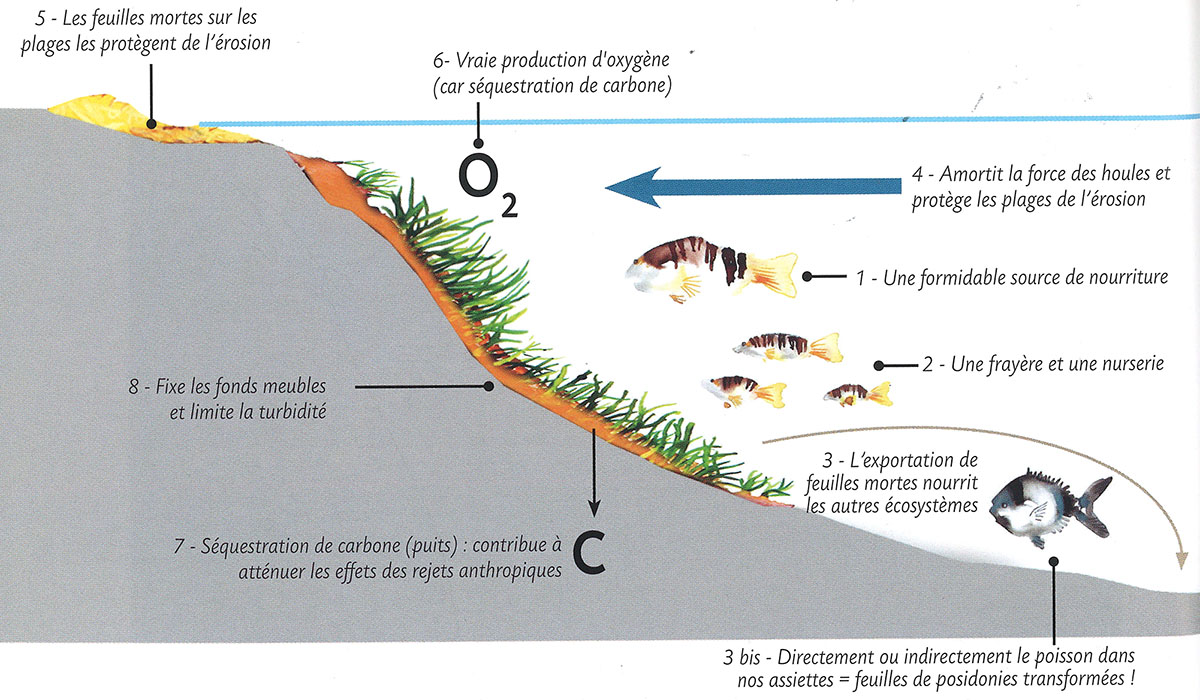
\includegraphics[width=\linewidth,keepaspectratio]{./1_intro/services_herbiers_posidonies_Boudouresque}
		\caption[Services écosystémiques fournis par les herbiers sous-marins]{Services écosystémiques fournis par les herbiers sous-marins (source : \href{https://planet-vie.ens.fr}{https://planet-vie.ens.fr}).}
	\label{figure_intro5}
\end{center}
\end{figure}

La posidonie (\textit{Posidonia oceanica}), une espèce protégée endémique de Méditerranée, forme de grandes prairies sous-marines entre la surface et 40 m de fond (\autoref{figure_intro6}). En raison de sa proximité à la côte et à la surface, cette espèce souffre tout particulièrement des effets des changements globaux \citep{marba_mediterranean_2014} et des pressions locales telles que l’augmentation de la population et de l’urbanisation côtières, responsables de la destruction et de la dégradation de cet habitat fragile \citep{montefalcone_human_2010, marba_mediterranean_2014, holon_impact_2015, telesca_seagrass_2015}. Les herbiers de posidonie sont reconnus comme un « habitat d’intérêt spécifique » en termes de biodiversité par la directive européenne concernant la conservation des habitats naturels ainsi que de la faune et de la flore sauvages (Directive Habitats 92/43/CEE).

%%%%%%%%%%%%%%%%%%%%%%%%%%%%%%%%%%%%%%%%%%%%%%%%%%%%%%%%%%
%%% Figure intro6: Illustrations herbiers de posidonie %%%
%%%%%%%%%%%%%%%%%%%%%%%%%%%%%%%%%%%%%%%%%%%%%%%%%%%%%%%%%%
\begin{figure}[H]
	\begin{center}
	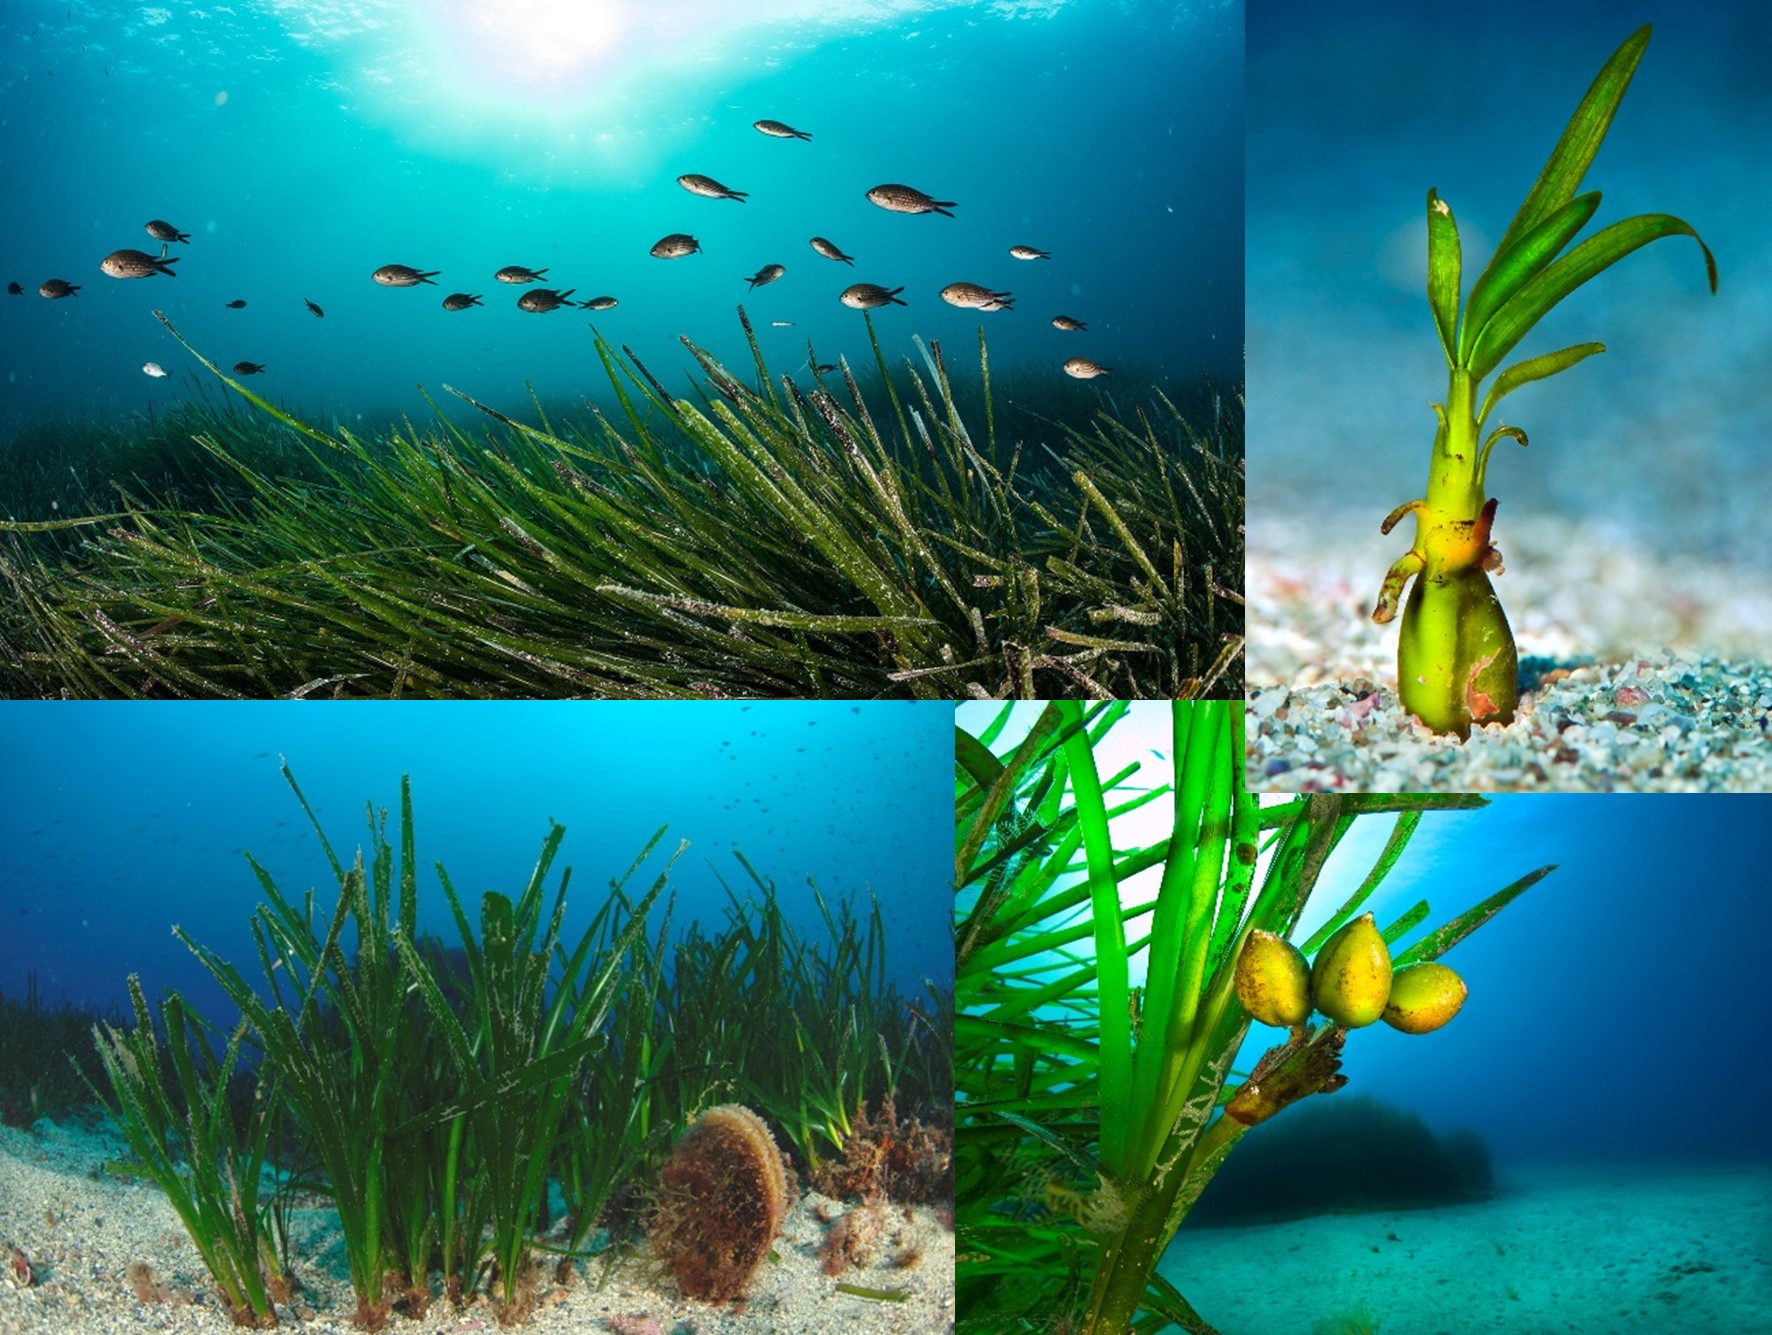
\includegraphics[width=\linewidth,keepaspectratio]{./1_intro/herbiers_posidonie}
		\caption[Illustrations d’un herbier de Posidonie]{Illustrations d’un herbier de Posidonie. De haut en bas et de gauche à droite : herbier avec quelques castagnoles (\textit{Chromis chromis}) ; graine germée de posidonie ; herbier avec une grande nacre (\textit{Pinna nobilis}) ; plant de posidonie avec ses graines) (\textit{©Andromède Océanologie}.}
	\label{figure_intro6}
\end{center}
\end{figure}

\subsubsection{Les récifs coralligènes : une biodiversité semblable aux récifs coralliens}\label{intro.1.3.2}

Les récifs coralligènes sont produits par l’accumulation de plus de 1500 espèces d’algues calcaires encroûtantes et d’animaux bioconstructeurs (polychètes, bryozoaires et gorgonaires) \citep{ballesteros_mediterranean_2006}; ce sont les seules formations calcaires d’origine biogénique en Méditerranée \citep{ballesteros_mediterranean_2006}, et leur diversité et productivité sont similaires à celles des récifs coralliens \citep{bianchi_biocostruzione_2001}. Ces récifs sont des niches écologiques importantes pour un grand nombre d’espèces mobiles : poissons, crustacés, échinodermes, mollusques, tuniqués \citep{ballesteros_mediterranean_2006} (\autoref{figure_intro7}). Comme les herbiers de posidonie, l’habitat « récifs coralligènes » est reconnu comme « habitat d’intérêt spécifique » en termes de biodiversité par la directive européenne concernant la conservation des habitats naturels ainsi que de la faune et de la flore sauvages (Directive Habitats 92/43/CEE).

%%%%%%%%%%%%%%%%%%%%%%%%%%%%%%%%%%%%%%%%%%%%%%%%%%%%%%%%
%%% Figure intro7: Illustrations récifs coralligènes %%%
%%%%%%%%%%%%%%%%%%%%%%%%%%%%%%%%%%%%%%%%%%%%%%%%%%%%%%%%
\begin{figure}[H]
	\begin{center}
	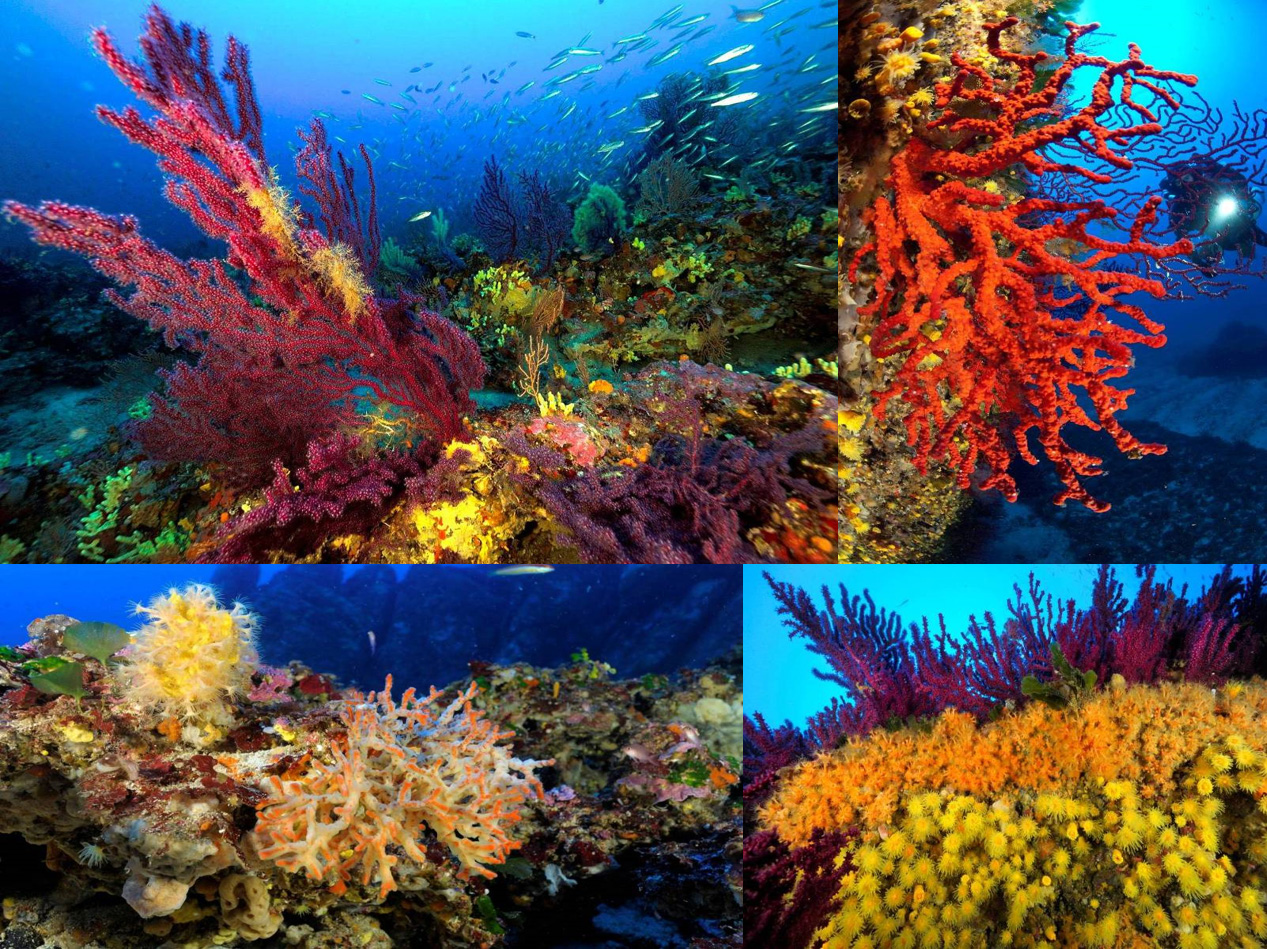
\includegraphics[width=\linewidth,keepaspectratio]{./1_intro/recifs_coralligenes}
		\caption[Illustrations des assemblages des récifs coralligènes]{Illustrations des assemblages des récifs coralligènes (\textit{©Andromède Océanologie}).}
	\label{figure_intro7}
\end{center}
\end{figure}

Bien que situés à des profondeurs allant de 12 à 120 m \citep{ballesteros_mediterranean_2006}, les récifs coralligènes ne sont pas exempts des effets des multiples pressions anthropiques qui affectent la biodiversité marine. Cet habitat est particulièrement affecté par l’accroissement de la sédimentation provoquée par les activités anthropiques côtières et les modifications de régimes hydro-sédimentaires \citep{airoldi_effects_2003}, ainsi que par la pêche et le mouillage \citep{ballesteros_mediterranean_2006}. 

\medskip

\setlength{\fboxsep}{5pt}
\setlength{\fboxrule}{0.6pt}
\noindent\framebox{%
  \begin{minipage}{\linewidth}
    La \textbf{biodiversité marine} est d’une \textbf{exceptionnelle richesse}, et l’humanité entière dépend des nombreux \textbf{services écosystémiques} qu’elle fournit. Pourtant, de nombreuses pressions anthropiques attaquent et érodent cette biodiversité, notamment en milieu côtier, où les densités de populations humaines et la biodiversité sont les plus élevées. \textbf{La Méditerranée} est le parfait exemple de cette co-occurrence de hauts niveaux de biodiversité et de pression, dans un espace géographique semi-fermé et restreint. La mise en place de \textbf{moyens de conservation efficaces} pour \textbf{préserver les écosystèmes marins} est aujourd’hui cruciale, mais la méconnaissance de ce milieu limite les actions visant à réduire son altération. Il est donc indispensable de \textbf{mettre en place des réseaux de surveillance} afin d’étudier et suivre l’état de santé des habitats marins, pour anticiper les changements et \textbf{assister les décisionnaires} dans la gestion de ces habitats.
  \end{minipage}}

\newpage

\section{Surveillance de la biodiversité marine}\label{intro.2}

Compte tenu de la crise climatique actuelle et de la sensibilité des assemblages marins aux diverses pressions anthropiques, il est nécessaire d’étudier et de suivre les dynamiques spatio-temporelles de la biodiversité marine afin de mettre en place des mesures de conservation efficaces \citep{magris_integrating_2014, klein_shortfalls_2015}. La surveillance globale de la biodiversité et de son évolution, notamment face aux changements climatiques, nécessite de s’accorder sur les \textbf{variables essentielles pour la biodiversité} (« Essential Biodiversity Variables », EBVs) à mesurer pour quantifier ces changements \citep{pereira_essential_2013, navarro_monitoring_2017, schmeller_operational_2017, haase_next_2018, kissling_building_2018}. L’intérêt de la conceptualisation des EBVs est né d’un besoin de structurer et d’harmoniser les données relatives à la surveillance de la biodiversité à différentes échelles spatiales et temporelles \citep{kissling_building_2018} afin de répondre aux objectifs de la Convention sur la Diversité Biologique (CDB 2010). Aujourd’hui, ces EBVs et les indicateurs qui en découlent doivent permettre de répondre aux besoins essentiels de la biodiversité dans le cadre de l’Agenda 2030 et ses objectifs de développement durable (Biodiversity and the 2030 Agenda for Sustainable Development). Elles constituent un premier niveau d’abstraction entre les \textbf{observations brutes} et les \textbf{indicateurs de biodiversité} ; on en distingue six classes : composition génétique, dynamique et distribution de populations, traits spécifiques, composition des communautés, fonctionnement et structure de l’écosystème \citep{pereira_essential_2013}. Dans le cadre de ce travail doctoral, nous nous concentrerons essentiellement sur la \textbf{distribution de populations}, la \textbf{composition des communautés} et la \textbf{structure de l’écosystème}.

\subsection{Indicateurs de biodiversité}\label{intro.2.1}

Si fondamentalement, elle cherche à caractériser la richesse biologique de notre planète, la notion de « biodiversité » semble bien complexe et protéiforme. En effet, elle inclut différentes échelles et différentes mesures quantitatives et qualitatives, il est donc extrêmement difficile de l’exprimer avec une seule métrique, et de très nombreux indices ont été développés \citep{teixeira_catalogue_2016}. Dans ce manuscrit, nous nous intéresserons à des indicateurs communs d’évaluation des assemblages écologiques ainsi qu’à des indicateurs originaux visant à décrire la structure de l’habitat. Plus particulièrement, nous utiliserons les indicateurs suivants pour caractériser les habitats marins :

\begin{itemize}
    \item \textbf{Diversité taxonomique} (ou « richesse spécifique ») : mesure la plus simple de la biodiversité, elle correspond au nombre d’espèces différentes observées dans un espace donné et à un moment donné. Ce nombre n’a jamais vocation à être exhaustif, et se limite souvent à ce qui est facilement observable (ex. : la diversité bactérienne est plus difficile à mesurer que la diversité d’oiseaux) ;
    
    \item \textbf{Indice de Shannon} \citep{magurran_measuring_2004} : semblable à la diversité taxonomique, il dépend non seulement du nombre d’espèces différentes observées, mais également de leur abondance relative. En effet, il convient de pouvoir distinguer deux communautés composées des mêmes espèces mais dont l’une aurait des abondances équitablement réparties entre espèces, et l’autre dominée par une ou plusieurs espèces. Cet indicateur reprend la forme de l’entropie, il est calculé comme suit :
    
    \begin{equation}
	    S_j=-\sum_{i}p_{ij} log(p_{ij})
	    \label{eqintro.1}
    \end{equation}
    
    Avec \textit{p\textsubscript{ij}} la prévalence de l’espèce $i$ au sein du site $j$.
    
    \item \textbf{Diversité fonctionnelle} : toutes les espèces présentent des caractéristiques morphologiques (taille, forme, biomasse…) et comportementales (relations trophiques, mode de reproduction, mobilité, migrations…) très différentes et parfois uniques, appelées « traits fonctionnels ». De fait, les espèces ne sont fonctionnellement pas équivalentes et il convient de pouvoir distinguer des assemblages en prenant en compte cette diversité, essentielle au bon fonctionnement des écosystèmes et à la provision de services écosystémiques dont dépendent les humains \citep{hooper_effects_2005, cadotte_using_2009, clemente_identifying_2010, faith_evosystem_2010}. Une multitude d’indices ont été développés afin de quantifier cette diversité fonctionnelle \citep{petchey_functional_2002, magurran_measuring_2004, mouchet_towards_2008, villeger_new_2008}~;
    
    \item \textbf{Structure de l’habitat} : si ses effets sur la biodiversité ne sont pas systématiquement négatifs (Fahrig, 2017), la \textbf{fragmentation} des habitats est connue pour jouer un rôle important dans la structuration et la dynamique des assemblages écologiques \citep{wilson_habitat_2016, crooks_quantification_2017}. La fragmentation peut se mesurer avec différents indicateurs paysagers \citep{de_montis_landscape_2017}. Par ailleurs, de nombreuses études ont montré que la \textbf{complexité structurale} de l’habitat avait un effet important sur la structuration des communautés, notamment l’abondance et la diversité des espèces marines \citep{luckhurst_analysis_1978, gratwicke_relationship_2005, harborne_biotic_2011, meager_topographic_2011, kovalenko_habitat_2012, graham_importance_2013, rees_abiotic_2014, darling_relationships_2017}. La complexité structurale se mesure généralement grâce à la \textbf{rugosité} de l’habitat \citep{friedman_multi-scale_2012, dustan_digital_2013, leon_measuring_2015} ou à sa \textbf{dimension fractale} \citep{yanovski_structural_2017, young_cost_2017, fukunaga_integrating_2019}.
    
\end{itemize}

\setlength{\fboxsep}{5pt}
\setlength{\fboxrule}{0.6pt}
\noindent\framebox{%
  \begin{minipage}{\linewidth}
    La \textbf{biodiversité} est une notion complexe \underline{qu’on ne peut pas synthétiser en un seul indicateur}. Dans le cas de \textbf{suivis écologiques} et l’étude des assemblages, il convient de mesurer différents compartiments et \textbf{calculer différents indicateurs} pour fournir une évaluation satisfaisante de \textbf{l’état d’un écosystème} et de son \textbf{fonctionnement}.
  \end{minipage}
}

\subsection[Méthodes d’acquisition d’images et de données cartographiques marines]{Méthodes d’acquisition d’images et de données \\cartographiques marines}\label{intro.2.2}

Afin d’évaluer la biodiversité marine et de quantifier les effets des pressions anthropiques, il est indispensable de \textbf{cartographier la présence} des espèces marines et de \textbf{quantifier leur abondance} à différentes échelles (principe des EBVs de distribution de populations) :

\begin{itemize}
    \item \textbf{Inventaires à méso/macro-échelle} avec une \underline{longue période de retour} pour étudier les facteurs environnementaux régissant la \underline{distribution des espèces}, et quantifier à plus large échelle les effets des pressions anthropiques ;
    
    \item \textbf{Inventaires à micro-échelle} avec une \underline{courte période de retour} pour comprendre la\\ \underline{complexité des assemblages} de certains habitats et détecter localement des changements précoces dans les équilibres écologiques.
\end{itemize}

Ces inventaires sont réalisés à l’aide de différentes méthodes d’acquisition, notamment des méthodes d’acquisition d’images qui permettent de déterminer la nature des assemblages et de cartographier l’étendue géographique des espèces. Si la colonne d’eau représente une forte contrainte pour l’étude des habitats marins, elle stimule le développement de méthodes cartographiques innovantes. Parmi elles, il convient de distinguer les méthodes cartographiques à méso/macro-échelle par télédétection, et à micro-échelle par proxy-détection et mesures \textit{in situ}.

\subsubsection{Cartographie à méso/macro-échelle par télédétection}\label{intro.2.2.1}

Plusieurs méthodes de télédétection sont utilisées pour cartographier les fonds marins à méso/\\macro-échelle : les images satellite et aériennes, les images sonar et sondeur, et les caméras tractées.

\paragraph{Imagerie satellite et aérienne}

L’accessibilité croissante d’images satellite gratuites avec des résolutions spatiales, temporelles et spectrales de plus en plus fines a permis d’élargir les applications de la télédétection à de nombreux domaines. Son utilisation s’est largement démocratisée en écologie terrestre, notamment à des fins de conservation avec la cartographie des EBVs \citep{pettorelli_framing_2016, luque_improving_2018, jetz_essential_2019}. Plus particulièrement, la télédétection permet aujourd’hui de cartographier la richesse spécifique des forêts \citep{feret_mapping_2014, vaglio_laurin_biodiversity_2014, baldeck_operational_2015} et la structure spatiale des communautés végétales \citep{rocchini_measuring_2018}. Elle est également utilisée pour d’autres applications environnementales, notamment en surveillance des océans \citep{devi_applications_2015} et des habitats marins \citep{hedley_remote_2016, mccarthy_satellite_2017, appolloni_use_2020, purkis_remote_2018}. Cependant, la télédétection satellitaire appliquée à la cartographie marine est contrainte par les propriétés absorbantes de l’eau et se limite aux habitats peu profonds et aux eaux claires \citep{purkis_remote_2018}. Par ailleurs, les conditions de mer et l’inclinaison du soleil au moment de l’acquisition doivent permettre de limiter la réflexion à la surface de l’eau pour pouvoir exploiter les images (mer calme et soleil au zénith). En eaux peu profondes et avec de bonnes conditions de mer, il est possible de cartographier finement des récifs coralliens ou des herbiers à l’aide d’images satellite (\autoref{figure_intro8}).

%%%%%%%%%%%%%%%%%%%%%%%%%%%%%%%%%%%%%%%%%%%%%
%%% Figure intro8: Télédétection herbiers %%%
%%%%%%%%%%%%%%%%%%%%%%%%%%%%%%%%%%%%%%%%%%%%%
\begin{figure}[H]
	\begin{center}
	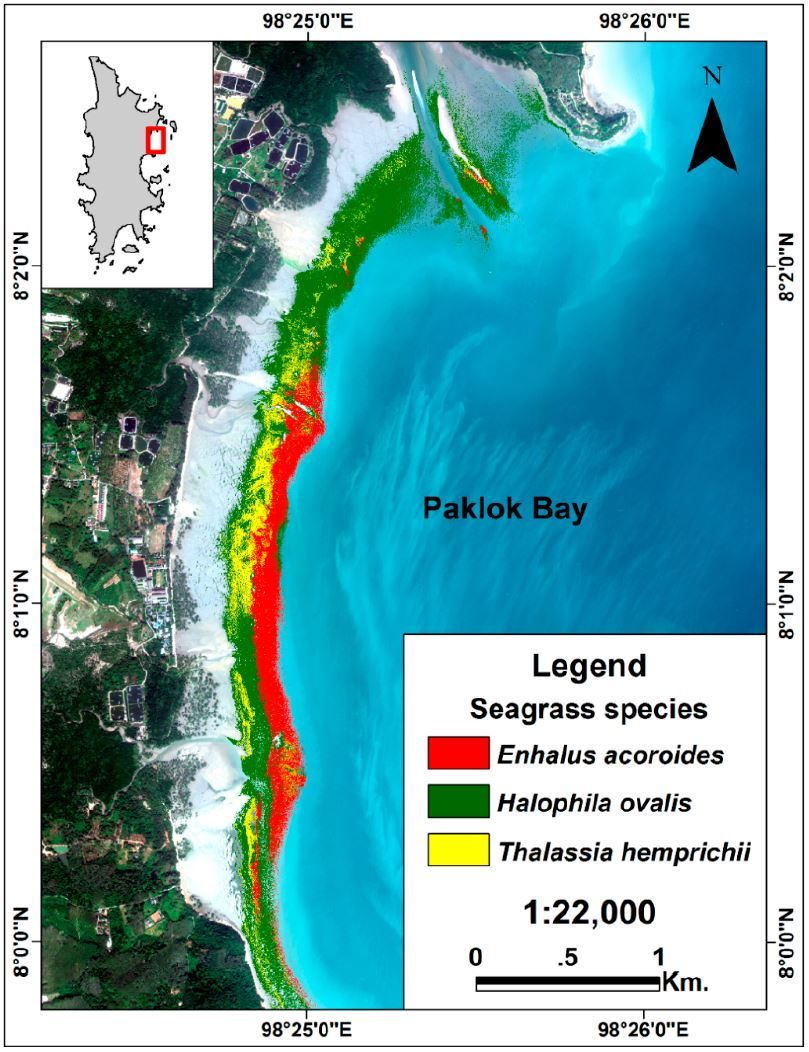
\includegraphics[width=0.7\linewidth,keepaspectratio]{./1_intro/remote_sensing_Koedsin2016}
		\caption[Exemple de cartographie d’herbiers sous-marins par télédétection]{Exemple de cartographie d’herbiers sous-marins dérivée d’images Worldview-2 et de données de référence \textit{in situ} en Thaïlande \citep{koedsin_integrated_2016}.}
	\label{figure_intro8}
\end{center}
\end{figure}

De façon similaire à la télédétection satellitaire, l’acquisition de données aériennes s’est largement développée en écologie grâce à la démocratisation des drones \citep{ivosevic_use_2015}, qui permettent d’acquérir à moindre coût des images aériennes à très haute résolution. Ce type d’image est notamment utilisé en milieu corallien pour cartographier les récifs \citep{casella_mapping_2017, collin_very_2018}.

\paragraph{Imageries sondeur et sonar : une échographie des fonds marins}

Bien que l’eau soit translucide, elle absorbe une grande proportion des rayons lumineux qui la traversent \citep{wozniak_light_2007}. Cette propriété limite considérablement les applications de la télédétection satellitaire et aérienne, qui n’est plus applicable dès lors que la profondeur ou la turbidité devient trop importante. Dans ce cas, la télédétection acoustique active (émission d’un signal de fréquence et d’intensité connues, et mesure de la réponse) à l’aide d’un capteur immergé représente une alternative à la télédétection satellite ou aérienne. Le sonar latéral et le sondeur multifaisceaux sont tous les deux des méthodes de télédétection acoustique active couramment utilisées pour cartographier les fonds marins \citep{saxena_review_1999, brown_benthic_2011} (\autoref{figure_intro9}). 

%%%%%%%%%%%%%%%%%%%%%%%%%%%%%%%%%%%%
%%% Figure intro9: Sonar sondeur %%%
%%%%%%%%%%%%%%%%%%%%%%%%%%%%%%%%%%%%
\begin{figure}[H]
	\begin{center}
	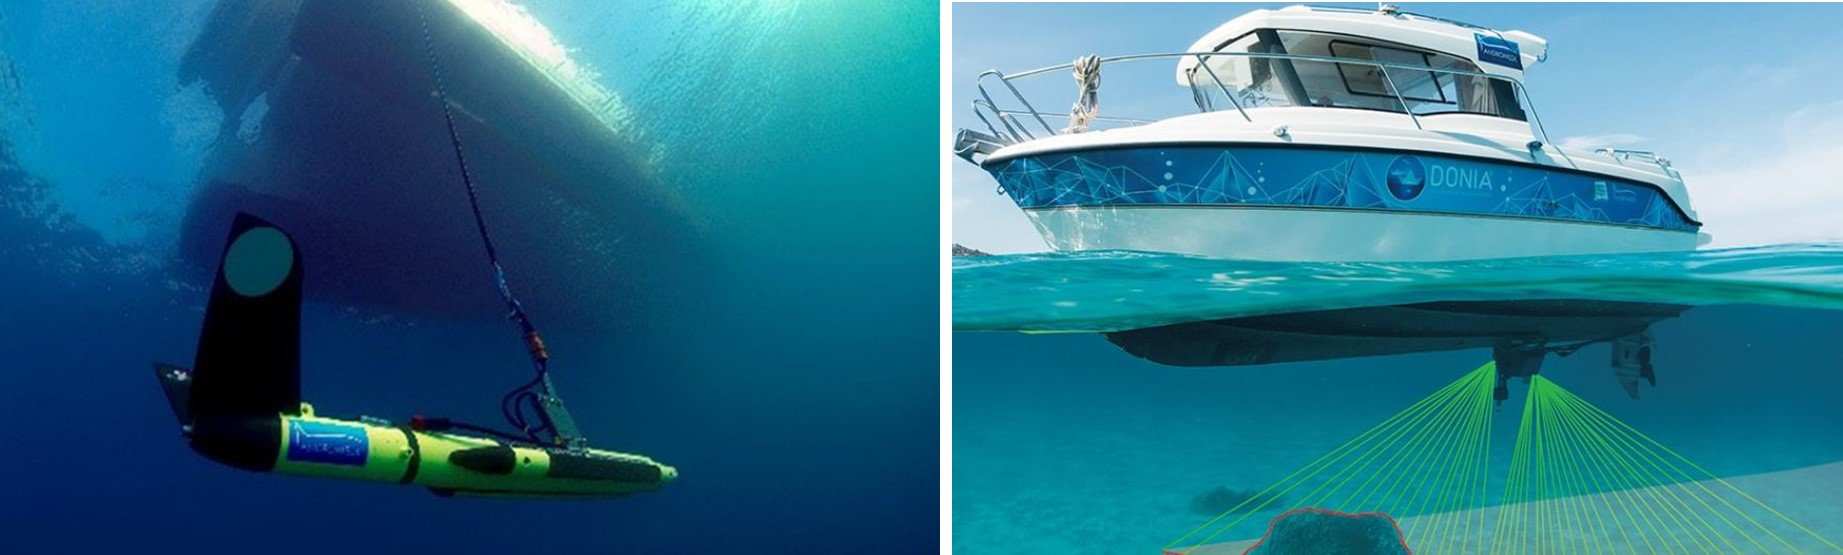
\includegraphics[width=\linewidth,keepaspectratio]{./1_intro/sonar_sondeur}
		\caption[Imagerie par sonar latéral et sondeur multifaisceaux]{Imagerie par sonar latéral (gauche) et sondeur multifaisceaux (droite) (\textit{©Andromède Océanologie}).}
	\label{figure_intro9}
\end{center}
\end{figure}

Si les deux techniques utilisent toutes deux l’acoustique, elles ne fonctionnent pas de la même manière et fournissent des résultats de natures différentes :

\begin{itemize}
    \item \textbf{Sonar latéral} : il émet un cône d’impulsions sonores d’environ 100 – 500 kHz en direction du fond et analyse l’intensité des réflexions avec une série d’hydrophones \citep{brown_benthic_2011}. Il en ressort une cartographie de l’état de surface et de la nature du fond, avec un signal d’autant plus fort que la surface du fond est dense et lisse (\autoref{figure_intro10} gauche);
    
    \item \textbf{Sondeur multifaisceaux} : il émet un cône d’impulsions sonores comme le sonar latéral, mais celui-ci mesure le temps mis par chaque impulsion pour traverser la colonne d’eau, se réfléchir sur le fond et revenir, et en déduit la profondeur en chaque point d’impact \citep{brown_benthic_2011}. Il en ressort une cartographie bathymétrique (\autoref{figure_intro10} droite).
    
\end{itemize}


%%%%%%%%%%%%%%%%%%%%%%%%%%%%%%%%%%%%%%%%%%%%%%%%%%
%%% Figure intro10: Acquisitions sonar sondeur %%%
%%%%%%%%%%%%%%%%%%%%%%%%%%%%%%%%%%%%%%%%%%%%%%%%%%
\begin{figure}[H]
	\begin{center}
	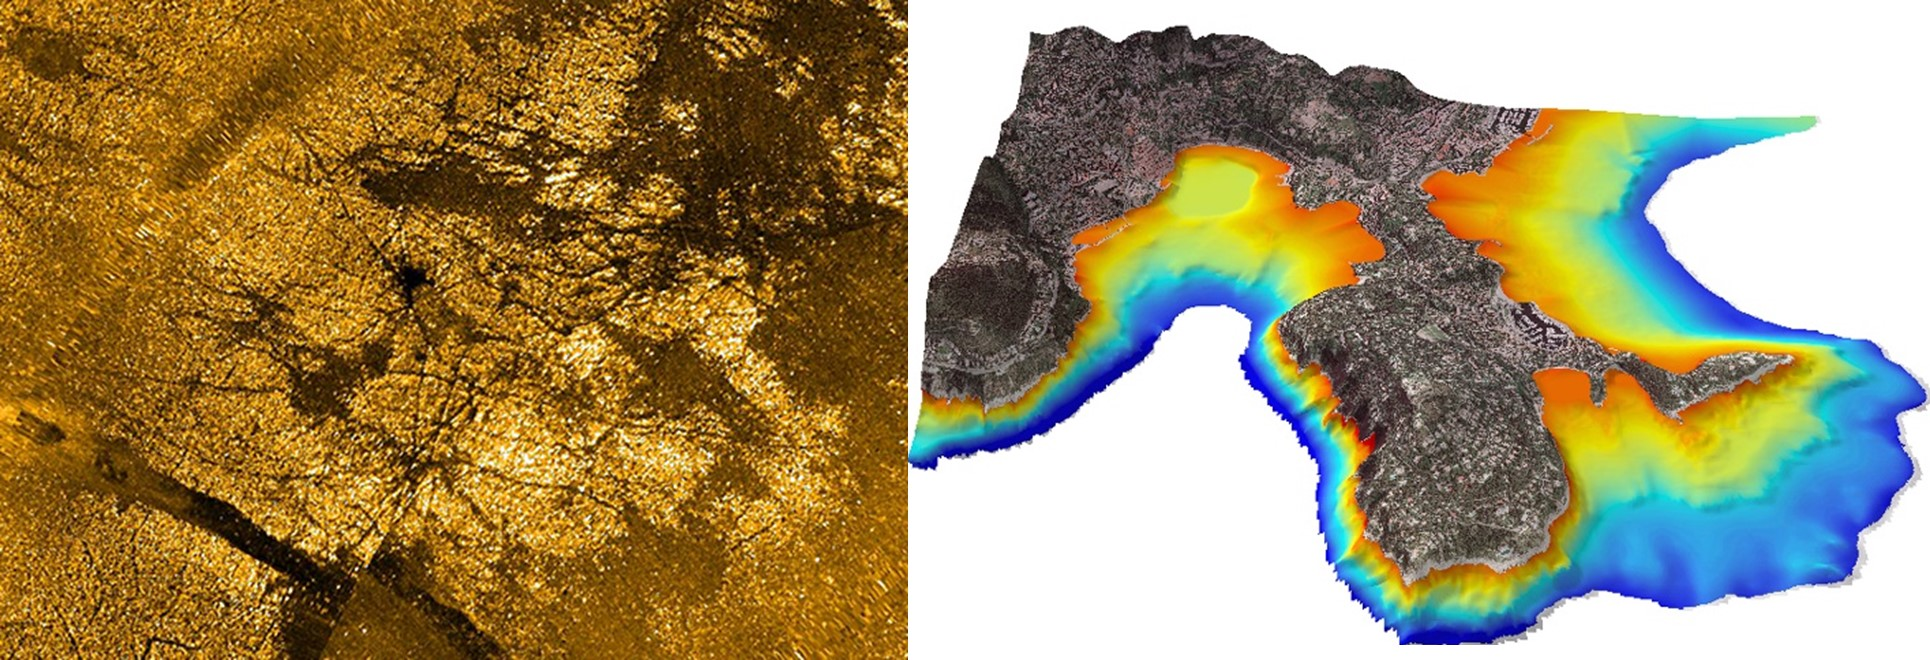
\includegraphics[width=\linewidth,keepaspectratio]{./1_intro/acquisitions_acoustiques}
		\caption[Exemples d’acquisitions acoustiques par sonar latéral et sondeur multifaisceaux]{Exemples d’acquisitions acoustiques par sonar latéral et sondeur multifaisceaux. À gauche : traces de mouillage dans l’herbier de posidonie visibles au sonar ; à droite : reproduction de la bathymétrie de Saint-Jean-Cap-Ferrat au sondeur multifaisceaux, le bleu correspondant aux zones les plus profondes (\textit{©Andromède Océanologie}).}
	\label{figure_intro10}
\end{center}
\end{figure}

Ces deux techniques sont complémentaires, elles permettent de définir des zones géographiques homogènes, identifiables par l’analyse de l’image sonar et par des observations \textit{in situ} collectées ponctuellement sur la zone d’étude \citep{brown_benthic_2011}. 

\paragraph{Caméra tractée}

De la même manière qu’un sonar est tracté derrière un bateau de sorte qu’il navigue à une dizaine de mètres au-dessus du fond, il est possible de tracter une caméra fixée sur un dispositif lui permettant de naviguer entre deux eaux et rester à distance réduite du fond \citep{rende_advances_2015}. Ce type d’acquisition photo ou vidéo permet de réaliser des assemblages photos ou des reconstructions trois dimensions (3D) des fonds par photogrammétrie et de cartographier les habitats de profondeur intermédiaire (10 – 40 m de profondeur). Comme pour le sonar latéral, il est possible d’estimer précisément la position géographique de la caméra à partir d’un positionnement GPS du bateau, du cap, de la longueur du câble et de la profondeur du dispositif (\autoref{figure_intro11}).

%%%%%%%%%%%%%%%%%%%%%%%%%%%%%%%%%%%%%%
%%% Figure intro11: Caméra tractée %%%
%%%%%%%%%%%%%%%%%%%%%%%%%%%%%%%%%%%%%%
\begin{figure}[H]
	\begin{center}
	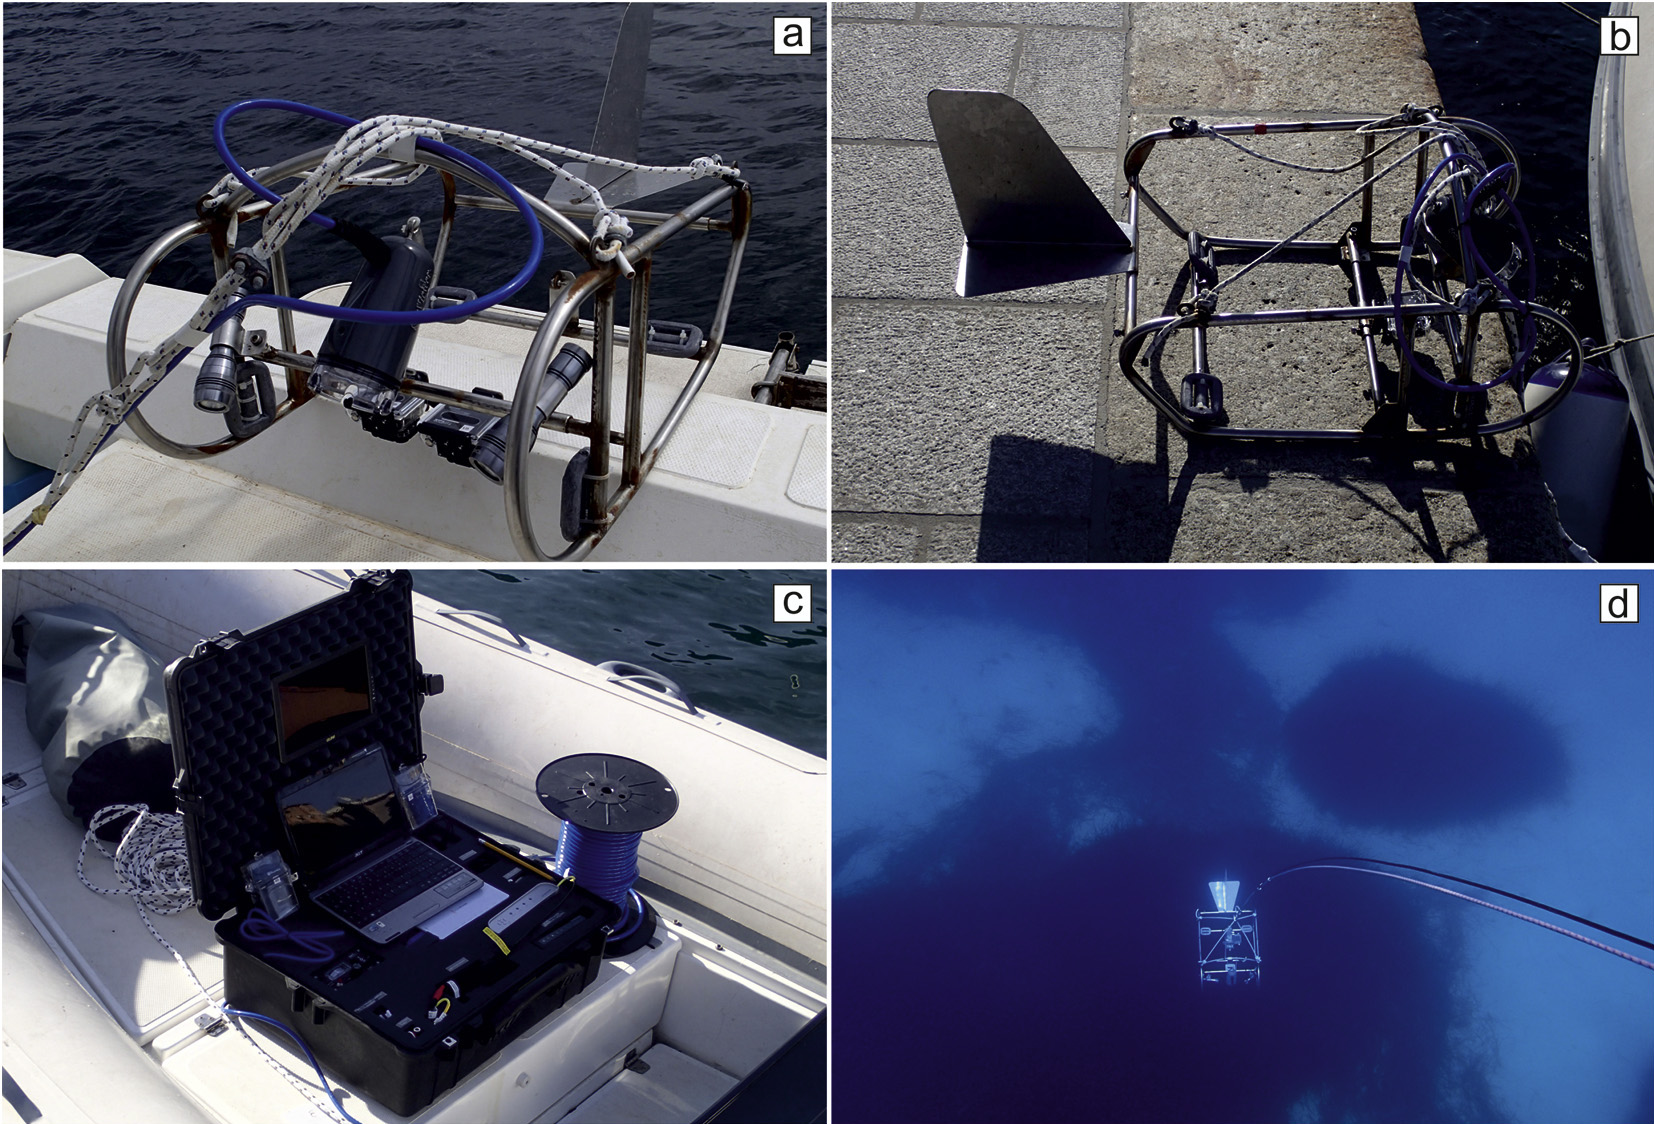
\includegraphics[width=0.7\linewidth,keepaspectratio]{./1_intro/towed_camera_Rende2015}
		\caption[Prototype de caméra tractée pour la cartographie d’habitats de profondeur intermédiaire]{Prototype de caméra tractée pour la cartographie d’habitats de profondeur intermédiaire \citep{rende_advances_2015}.}
	\label{figure_intro11}
\end{center}
\end{figure}

\setlength{\fboxsep}{5pt}
\setlength{\fboxrule}{0.6pt}
\noindent\framebox{%
  \begin{minipage}{\linewidth}
    Si les données obtenues par télédétection, quelle que soit leur nature, permettent de réaliser des cartographies à \textbf{méso/macro-échelle} pour un \textbf{coût et un temps d’acquisition relativement faibles}, elles ne permettent pas d’étudier les phénomènes écologiques qui se produisent à \textbf{micro-échelle} ni de suivre la \textbf{composition des assemblages} dans le temps.
  \end{minipage}
}

\subsubsection{Cartographie micro-échelle par proxy-détection et mesures in situ}\label{intro.2.2.2}

Si la télédétection permet d’étudier la répartition des espèces et des habitats dans l’espace, certaines études nécessitent de collecter de la donnée cartographique à plus fine échelle, comme la reconnaissance d’espèces et des mesures de tailles. Pour ces études, il est possible de réaliser des mesures \textit{in situ} ou à proximité (proxy-détection) en rapprochant le capteur du sujet.

\paragraph{Relevés plongeur}

À l’instar des relevés terrain terrestres (botanique, géologie…), l’acquisition de données peut être réalisée par le biologiste en milieu sous-marin à l’aide d’outils de plongée. Si la plongée en apnée ou sous cloche existe depuis l’Antiquité, il faudra attendre la fin du 18e siècle pour voir arriver les premiers scaphandres permettant de plus longues immersions. Plus récemment, la plongée militaire et la plongée technique ont contribué à mettre au point des scaphandres recycleurs autonomes permettant de rester plusieurs heures sous l’eau et d’atteindre des profondeurs pouvant dépasser les 100 m de fond \citep{sieber_review_2010}. Parmi la multitude de protocoles possibles, la plongée permet notamment de réaliser des relevés photographiques et de cartographier les habitats par télémétrie acoustique.

\noindent\textbf{Relevés photographiques}

Les relevés photographiques \textit{in situ} permettent de rendre compte de l’état d’un habitat à un instant donné, et de produire une évaluation qualitative (rendu visuel) ou quantitative (analyse ou interprétation d’images). Ils permettent de réaliser des assemblages photos 2D ou des reconstructions 3D (par photogrammétrie) afin de cartographier les habitats, quantifier le fractionnement, positionner les différentes espèces dans l’espace, et assurer un suivi dans le temps. Par ailleurs, la standardisation des conditions d’acquisition (distance, éclairement) permet de définir des protocoles d’échantillonnage par quadrats photographiques pour évaluer et suivre la biodiversité des habitats benthiques \citep{deter_rapid_2012} (\autoref{figure_intro12}).

%%%%%%%%%%%%%%%%%%%%%%%%%%%%%%%%%%%%%%%%%%%%%%
%%% Figure intro12: Quadrat photographique %%%
%%%%%%%%%%%%%%%%%%%%%%%%%%%%%%%%%%%%%%%%%%%%%%
\begin{figure}[H]
	\begin{center}
	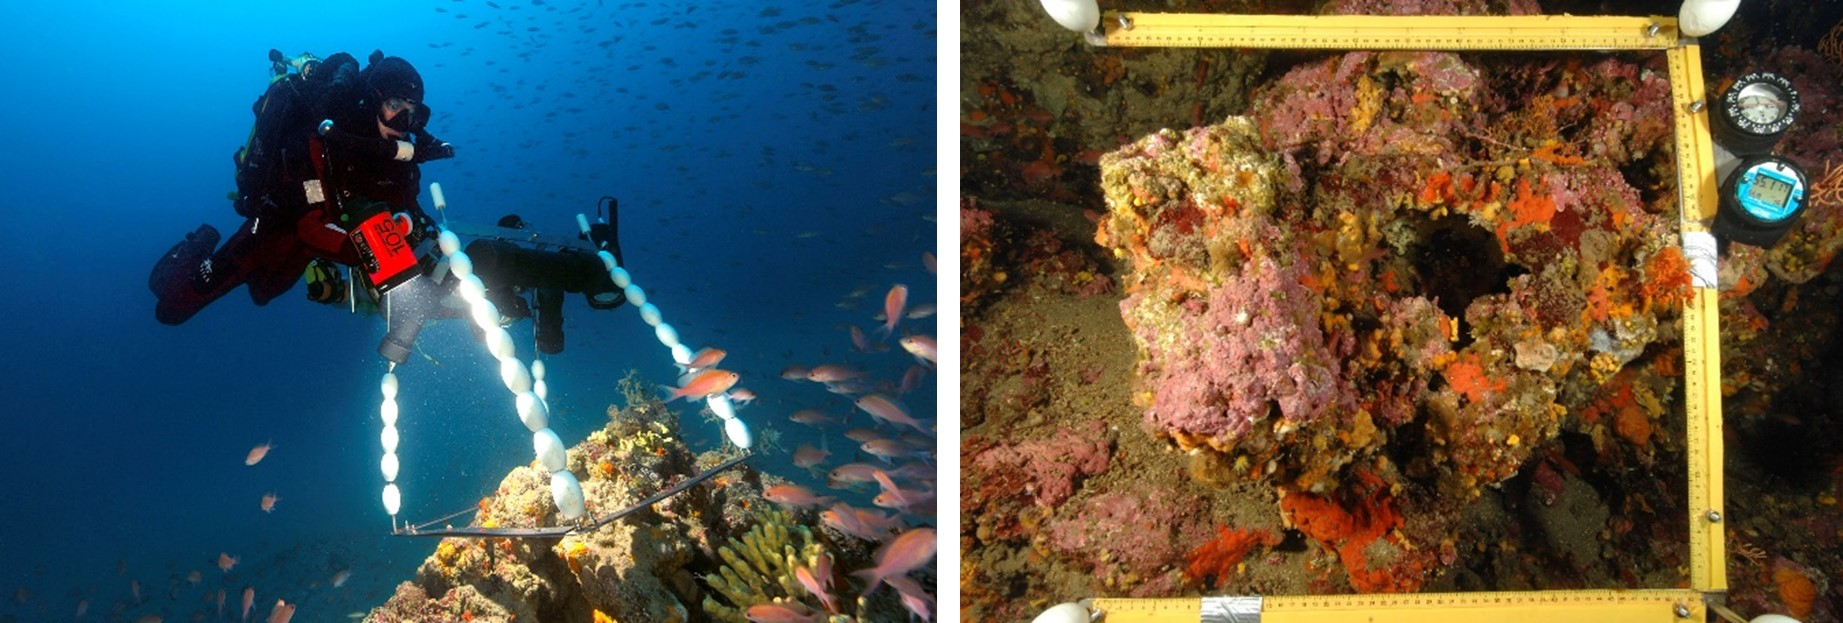
\includegraphics[width=\linewidth,keepaspectratio]{./1_intro/quadrat}
		\caption[Quadrat photographique permettant l’analyse de la biodiversité benthique par un taxonomiste]{Quadrat photographique permettant l’analyse de la biodiversité benthique par un taxonomiste (\textit{©Andromède Océanologie}).}
	\label{figure_intro12}
\end{center}
\end{figure}

\noindent\textbf{Cartographie par télémétrie acoustique}

Le signal GPS n’étant pas disponible sous l’eau, le positionnement est nécessairement relatif à une position connue (par cartographie sondeur préalable, position en surface ou bien référentiel arbitraire) et déterminé par interférométrie acoustique Ultra-Short Base Line (USBL). Ce type de technologie permet de mesurer un cap et une distance entre un émetteur et un récepteur, et donc de connaître la position d’un objet relativement à un point fixe. À l’aide de cette technologie, il est possible de cartographier des habitats marins sur une surface réduite (quelques dizaines à quelques centaines de m²) en disposant une antenne de réception fixe et en pointant la limite des objets avec un émetteur (\autoref{figure_intro13}). Les cartographies produites à différents pas de temps peuvent ensuite être géoréférencées à l’aide de points de position géographique connue (roches, aménagements…) ou bien simplement alignées et comparées, par exemple dans le cas de suivis temporels d’herbiers de posidonie \citep{descamp_underwater_2005, descamp_fast_2011}.

%%%%%%%%%%%%%%%%%%%%%%%%%%%%%%%%%%%%%%%%%%%%%
%%% Figure intro13: Télémétrie acoustique %%%
%%%%%%%%%%%%%%%%%%%%%%%%%%%%%%%%%%%%%%%%%%%%%
\begin{figure}[H]
	\begin{center}
	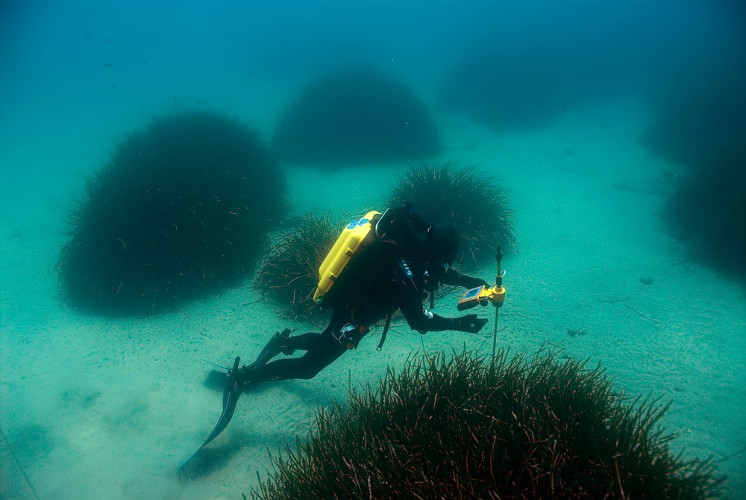
\includegraphics[width=0.8\linewidth,keepaspectratio]{./1_intro/telemetrie}
		\caption[Plongeur entrain de cartographier un herbier de posidonie à l’aide d’un télémètre acoustique]{Plongeur entrain de cartographier un herbier de posidonie à l’aide d’un télémètre acoustique (\textit{©Andromède Océanologie}).}
	\label{figure_intro13}
\end{center}
\end{figure}

\setlength{\fboxsep}{5pt}
\setlength{\fboxrule}{0.6pt}
\noindent\framebox{%
  \begin{minipage}{\linewidth}
    Si la plongée scientifique permet au naturaliste de faire lui-même ses observations et d’acquérir de la \textbf{donnée très fine}, elle est malheureusement contrainte par la \textbf{physiologique humaine} et les temps de décompression, qui augmentent exponentiellement avec la profondeur et peuvent pénaliser un plongeur durant \textbf{plusieurs heures} pour \textbf{quelques dizaines de minutes de travail} au fond. C’est pourquoi dans les cas extrêmes ou lorsque la complexité de la tâche le permet, les robots sont préférés aux plongeurs.
  \end{minipage}
}

\paragraph{Les robots: ROV et AUV}

Les robots sous-marins sont des plateformes mobiles au service de l’utilisateur, souvent adaptables pour la tâche souhaitée en les équipant du capteur ou de l’outil adéquat pour mener à bien sa mission. Si le coup de mise en œuvre est généralement élevé par rapport à un plongeur (coût du robot et déploiement par un navire océanographique adéquat), ils peuvent travailler plus profond (jusqu’à plusieurs centaines de mètres) et sans limites de temps due à la physiologie. Il en existe deux sortes : les Remotely Operated Vehicles (ROVs) et les Autonomous Underwater Vehicles (AUVs) \citep{bogue_underwater_2015}. Les ROVs sont téléopérés depuis la surface par un câble, appelé communément « ombilical », de diamètre variable selon qu’il véhicule uniquement les ordres de navigation ou bien également l’alimentation électrique. Si l’ombilical qui les relie au navire leur confère un certain handicap, il est possible de les piloter en temps réel et d’adapter la navigation et l’acquisition de données en fonction de ce que voit le pilote en surface (\autoref{figure_intro14}).

%%%%%%%%%%%%%%%%%%%%%%%%%%%%%
%%% Figure intro14: ROV3D %%%
%%%%%%%%%%%%%%%%%%%%%%%%%%%%%
\begin{figure}[H]
	\begin{center}
	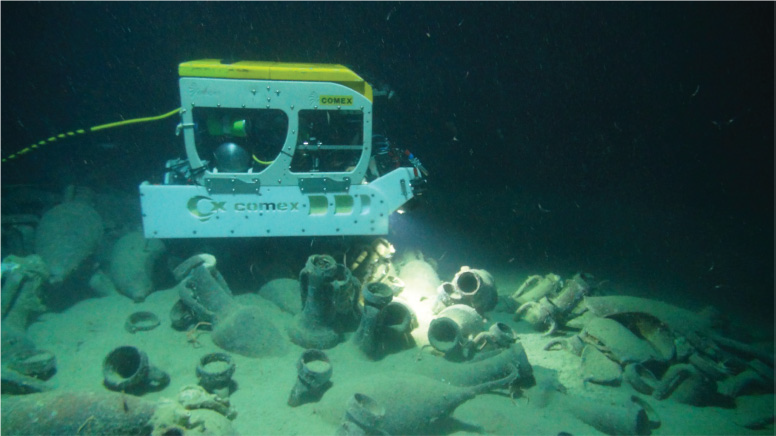
\includegraphics[width=0.7\linewidth,keepaspectratio]{./1_intro/ROV3D_Drap2015}
		\caption[ROV3D : un robot d’acquisition photogrammétrique pour l’archéologie sous-marine]{ROV3D : un robot d’acquisition photogrammétrique pour l’archéologie sous-marine \citep{drap_rov_2015}.}
	\label{figure_intro14}
\end{center}
\end{figure}

Comme leur nom l’indique, les AUVs sont autonomes et doivent donc être programmés pour réaliser un parcours d’acquisition précis et maintenir une distance au fond tout en évitant les éventuels obstacles, en utilisant des technologies de positionnement \citep{johnson-roberson_generation_2010, bonin-font_towards_2016} (\autoref{figure_intro15}). Ces robots permettent de réaliser des acquisitions de manière entièrement autonome une fois déployés, mais ils requièrent une technologie et un temps de développement généralement beaucoup plus onéreux que les ROVs.

%%%%%%%%%%%%%%%%%%%%%%%%%%%
%%% Figure intro15: AUV %%%
%%%%%%%%%%%%%%%%%%%%%%%%%%%
\begin{figure}[H]
	\begin{center}
	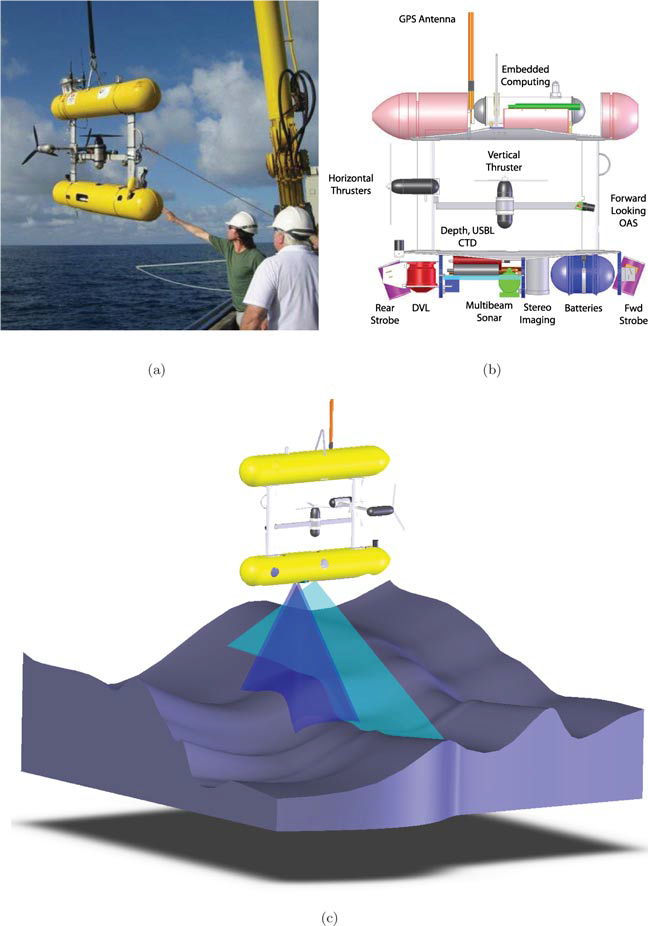
\includegraphics[width=0.7\linewidth,keepaspectratio]{./1_intro/AUV_Johnson-Roberson2010}
		\caption[Exemple d’un robot autonome (AUV) pour de l’acquisition d’images à grande échelle]{Exemple d’un robot autonome (AUV) pour de l’acquisition d’images à grande échelle \citep{johnson-roberson_generation_2010}.}
	\label{figure_intro15}
\end{center}
\end{figure}

\setlength{\fboxsep}{5pt}
\setlength{\fboxrule}{0.6pt}
\noindent\framebox{%
  \begin{minipage}{\linewidth}
    Les robots sous-marins sont d’excellents outils pour acquérir des données photographiques sur de \textbf{grandes surfaces} (AUV) ou à de \textbf{grandes profondeurs} (ROV) ; mais leur maniabilité réduite, leur coût de développement et leur mise en œuvre rendent bien souvent le \textbf{plongeur autonome plus pertinent} et compétitif (jusqu’à une certaine profondeur), notamment depuis la démocratisation des scaphandres recycleurs. 
  \end{minipage}
}

\subsection{Les réseaux de surveillance en Méditerranée française}\label{intro.2.3}

Les réseaux de surveillance ont pour objectif le suivi écologique de certains habitats ou espèces à l’échelle régionale ou globale, en standardisant les méthodes de collecte et de traitement de données. L’analyse des données de ces réseaux permet de comparer la qualité écologique des différentes stations de suivis et de mesurer leur évolution dans le temps, afin de mettre en œuvre des mesures de gestion efficaces. De nombreux réseaux de surveillance existent en Méditerranée française, dont une partie est financée par l’Agence de l’Eau Rhône-Méditerranée-Corse, et sont rassemblés sur la plateforme cartographique « Medtrix » (\href{https://medtrix.fr/}{https://medtrix.fr/}). Deux de ces réseaux sont gérés par la société Andromède Océanologie et concernent les habitats les plus riches et les plus sensibles de Méditerranée : les herbiers de posidonie (TEMPO) et les récifs coralligènes (RECOR).

\subsubsection{La société Andromède Océanologie}\label{intro.2.3.1}

Andromède Océanologie (\href{www.andromede-ocean.com}{www.andromede-ocean.com}) est une PME créée en 2008, spécialisée dans les relevés écologiques \textit{in situ} en plongée sous-marine. Son objectif est de conduire des projets innovants liés à l'étude et à la valorisation de l'environnement marin. Les activités d’Andromède Océanologie et de son équipe de 13 personnes sont organisées en 3 pôles : 

\begin{itemize}
    \item \textbf{Un pôle bureau d’études} dont les capacités d’expertise ont notamment trait à la bathymétrie, la cartographie des biocénoses marines, l’analyse écologique et la gestion des écosystèmes marins~;
    
    \item \textbf{Un pôle valorisation} qui gère notamment la diapothèque (plus de 25 000 clichés) de Laurent Ballesta, plongeur extrême et photographe sous-marin internationalement reconnu, auteur de nombreux livres, documentaires et expéditions~;
    
    \item \textbf{Un pôle Recherche et Développement} qui met au point des technologies innovantes pour l’évaluation, le suivi et l’amélioration de l’état de santé des écosystèmes marins côtiers. Andromède porte ainsi plusieurs réseaux de surveillance de l’état écologique des eaux côtières, en partenariat avec l’Agence de l’Eau Rhône Méditerranée Corse. Par ailleurs, un programme de « laboratoire commun » mutualise les moyens et efforts de recherche entre la société et l’Université de Montpellier (UMR MARBEC) pour le développement de méthodes d’observations innovantes sur les habitats méditerranéens\\ (\href{https://labcomintosea.edu.umontpellier.fr}{https://labcomintosea.edu.umontpellier.fr}).
\end{itemize}

La société est localisée en bord de mer à Carnon (Occitanie, France), et dispose d’un parc matériel et technologique très spécialisé consacré aux domaines de l'océanologie et de la plongée hi Tech : trois bateaux, sonar latéral, sondeur multifaisceaux, système de positionnement GPS-rtk, scaphandres de plongée à circuit ouvert et fermé (recycleur), équipement photo et vidéo sous-marines pour films professionnels, etc. Andromède Océanologie a réalisé la plupart des cartographies des biocénoses marines côtières (0 à 80 m de fond) de Méditerranée française et quelques zones à l’étranger (ilots de Galite et Zembra en Tunisie, réserves de Tavolara et Carbonara en Sardaigne (Italie), réserve de Karaburun - Sazan en Albanie, etc.). Elle est à l’origine de la première cartographie continue des biocénoses (1 : 10 000) en Méditerranée française (Andromède Océanologie, 2014). Ces cartes sont mises gratuitement à la disposition des professionnels de la mer sur la plateforme cartographique Medtrix (\href{https://plateforme.medtrix.fr/}{https://plateforme.medtrix.fr/}) dans le projet DONIA Expert. Une version simplifiée de ces cartes est disponible sur l’application mobile de plaisance Donia : ancrage en toute sécurité et hors des habitats sensibles, cartes 3D des fonds pour repérer les sites de plongée ou de pêche, outil de navigation communautaire… (\href{https://donia.fr/}{https://donia.fr/}) Cette application gratuite a reçu le prix Bateau Bleu et le prix Entreprises et Biodiversité de 2013, et a fait l’objet d’une mise à jour (version 5.0) importante en 2020 (ajout de données et d’outils, amélioration de l’ergonomie).

\subsubsection{TEMPO : un réseau de surveillance des herbiers de posidonie en Méditerranée française}\label{intro.2.3.2}

Les herbiers sous-marins sont de bons indicateurs des conditions environnementales : une perturbation de leur distribution traduit des changements environnementaux \citep{orth_global_2006}. Plus particulièrement, la posidonie, qui pousse à des profondeurs allant de la surface jusqu’à plus de 40 m de fond en fonction de la clarté de l’eau, est couramment utilisée comme un bio-indicateur de la qualité de l’eau, entre autres à travers l’évolution de sa limite inférieure (i.e. limite profonde au-delà de laquelle les conditions favorables à sa croissance ne sont plus réunies) \citep{boudouresque_regression_2009, ruiz_mediterranean_2009}. En effet, la profondeur de la limite inférieure est principalement déterminée par la clarté de l’eau, et représente un indicateur robuste de l’état global de l’ensemble de l’écosystème \citep{borum_european_2004}. Par ailleurs, il est important de prendre en compte des mesures quantitatives de la vitalité de l’herbier à une profondeur identique (-15 m ; profondeur représentative de l’herbier en Méditerranée), car les herbiers peu profonds montrent une grande variabilité naturelle \citep{marba_interannual_1997, balestri_spatial_2003}. Des indicateurs intègrent les différentes mesures de vitalité de l’herbier (densité, longueurs de feuilles, épiphytes…) et des espèces associées (herbivores, échinodermes, filtreurs, prédateurs…), afin d’évaluer le fonctionnement global de l’herbier, à la fois à la profondeur intermédiaire et en limite inférieure.

TEMPO est un réseau de surveillance de l’état écologique des herbiers de posidonie en Méditerranée française qui intègre ces deux composantes importantes de l’herbier : la limite inférieure et la profondeur intermédiaire. Ce réseau est opéré par Andromède océanologie, depuis 2011, avec le soutien de l’Agence de l’Eau Rhône-Méditerranée-Corse. La caractérisation de l’état écologique de l’herbier est réalisée par une campagne régionale annuelle sur la période mi-mai / fin juin. Chaque année, une des trois régions concernées par cette agence de l’eau (Corse, région Sud-Provence-Alpes Côte d’Azur et Occitanie) est échantillonnée, avec un roulement sur trois ans. Toutes régions confondues, le réseau TEMPO permet au total l’échantillonnage de 96 sites d’herbier dont 47 sites sont localisés à la profondeur intermédiaire et 53 en limite inférieure (quatre limites inférieures peu profondes sont aussi considérées comme sites à la profondeur intermédiaire), le plus souvent dans l’alignement des sites à profondeur intermédiaire (\autoref{figure_intro16}). 

%%%%%%%%%%%%%%%%%%%%%%%%%%%%%%%%%%%%%%%
%%% Figure intro16: le réseau TEMPO %%%
%%%%%%%%%%%%%%%%%%%%%%%%%%%%%%%%%%%%%%%
\begin{figure}[H]
	\begin{center}
	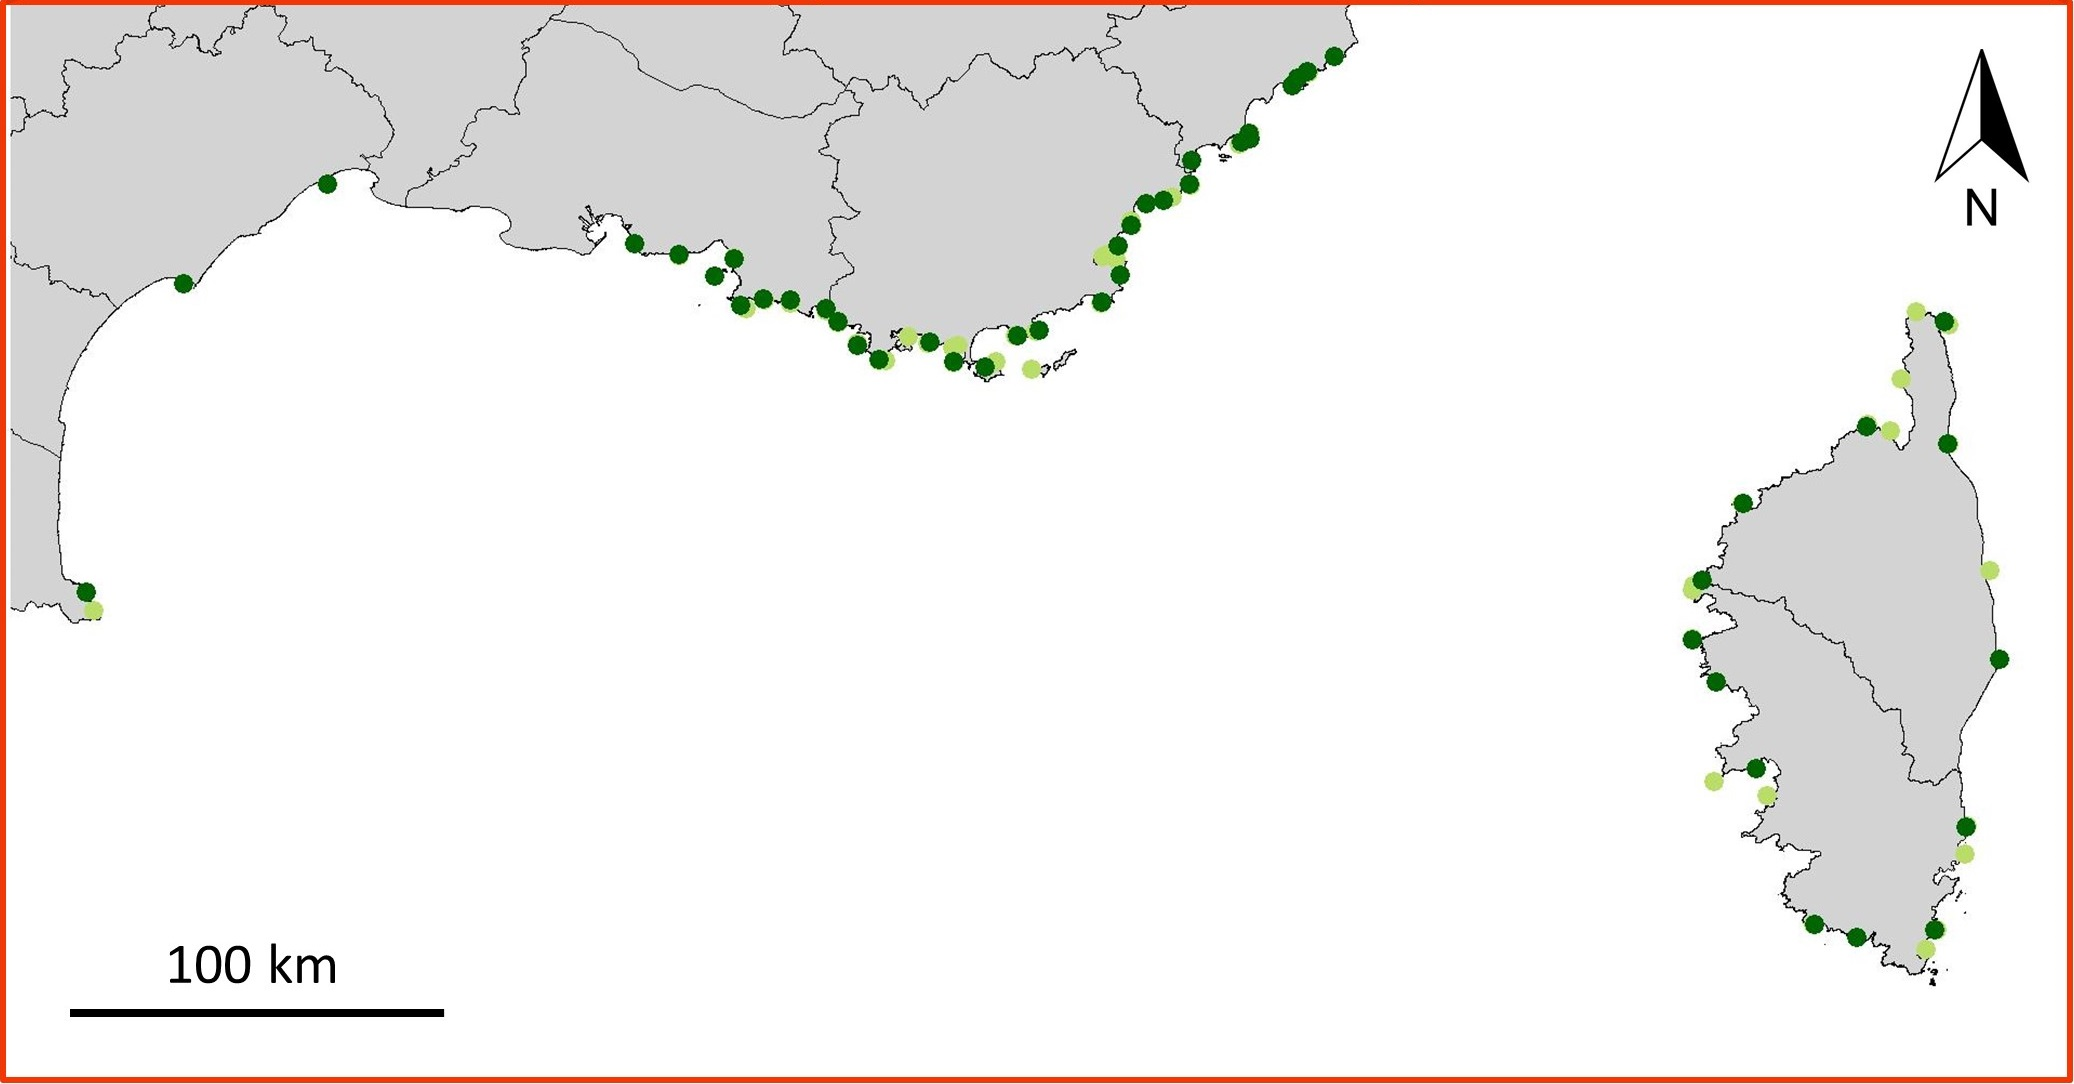
\includegraphics[width=\linewidth,keepaspectratio]{./1_intro/reseau_TEMPO}
		\caption[Localisation des sites du réseau de surveillance TEMPO]{Localisation des sites du réseau de surveillance TEMPO. En vert clair: les 47 sites à -15m ; en vert foncé: les 53 sites en limite inférieure.}
	\label{figure_intro16}
\end{center}
\end{figure}

La méthode choisie pour la surveillance de l’herbier de posidonie en limite inférieure prend en compte deux types de mesures : une cartographie de la limite inférieure de l’herbier par télémétrie acoustique, et des mesures de vitalité de l’herbier. La méthode de télémétrie acoustique permet à l’opérateur d’effectuer un point tous les 30 à 50 cm pour cartographier précisément la limite inférieure grâce à l’Aquamètre D100-NG dernière génération (\href{http://www.plsm.eu}{http://www.plsm.eu}) relié à une tablette tactile étanche. La caractérisation de l’état de conservation des herbiers de Posidonia oceanica est réalisée selon les protocoles standardisés du PREI \citep{gobert_assessment_2009}, de l’EBQI \citep{personnic_ecosystem-based_2014} et du BiPo \citep{lopez_y_royo_biotic_2010} basés sur des mesures biologiques in situ et en laboratoire. Par ailleurs, des mesures bioacoustiques sont réalisées sur certains sites afin de quantifier l’activité des espèces mobiles (en partenariat avec l’équipe de Chorus (\href{https://chorusacoustics.com/}{https://chorusacoustics.com/}) qui porte le réseau de surveillance CALME) (\autoref{figure_intro17}).

\medskip 

\setlength{\fboxsep}{5pt}
\setlength{\fboxrule}{0.6pt}
\noindent\framebox{%
  \begin{minipage}{\linewidth}
    Le protocole TEMPO permet d’acquérir une \textbf{diversité de mesures de vitalité de l’herbier} à la \textbf{profondeur intermédiaire} (-15 m) et en \textbf{limite inférieure}, ainsi que des \textbf{espèces associées} (filtreurs, herbivores…). Si la cartographie de la limite inférieure par \textbf{télémétrie acoustique} permet de suivre finement son \textbf{évolution dans le temps}, la résolution dépend de la volonté du plongeur, et la manipulation peut être longue et devenir \textbf{physiologiquement contraignante} pour le plongeur dans le cas des herbiers les plus \textbf{profonds} (notamment en Corse) et les plus \textbf{fragmentés}.
  \end{minipage}
}

%%%%%%%%%%%%%%%%%%%%%%%%%%%%%%%%%%%%%%%%
%%% Figure intro17: la méthode TEMPO %%%
%%%%%%%%%%%%%%%%%%%%%%%%%%%%%%%%%%%%%%%%
\begin{sidewaysfigure}
\begin{figure}[H]
	\begin{center}
	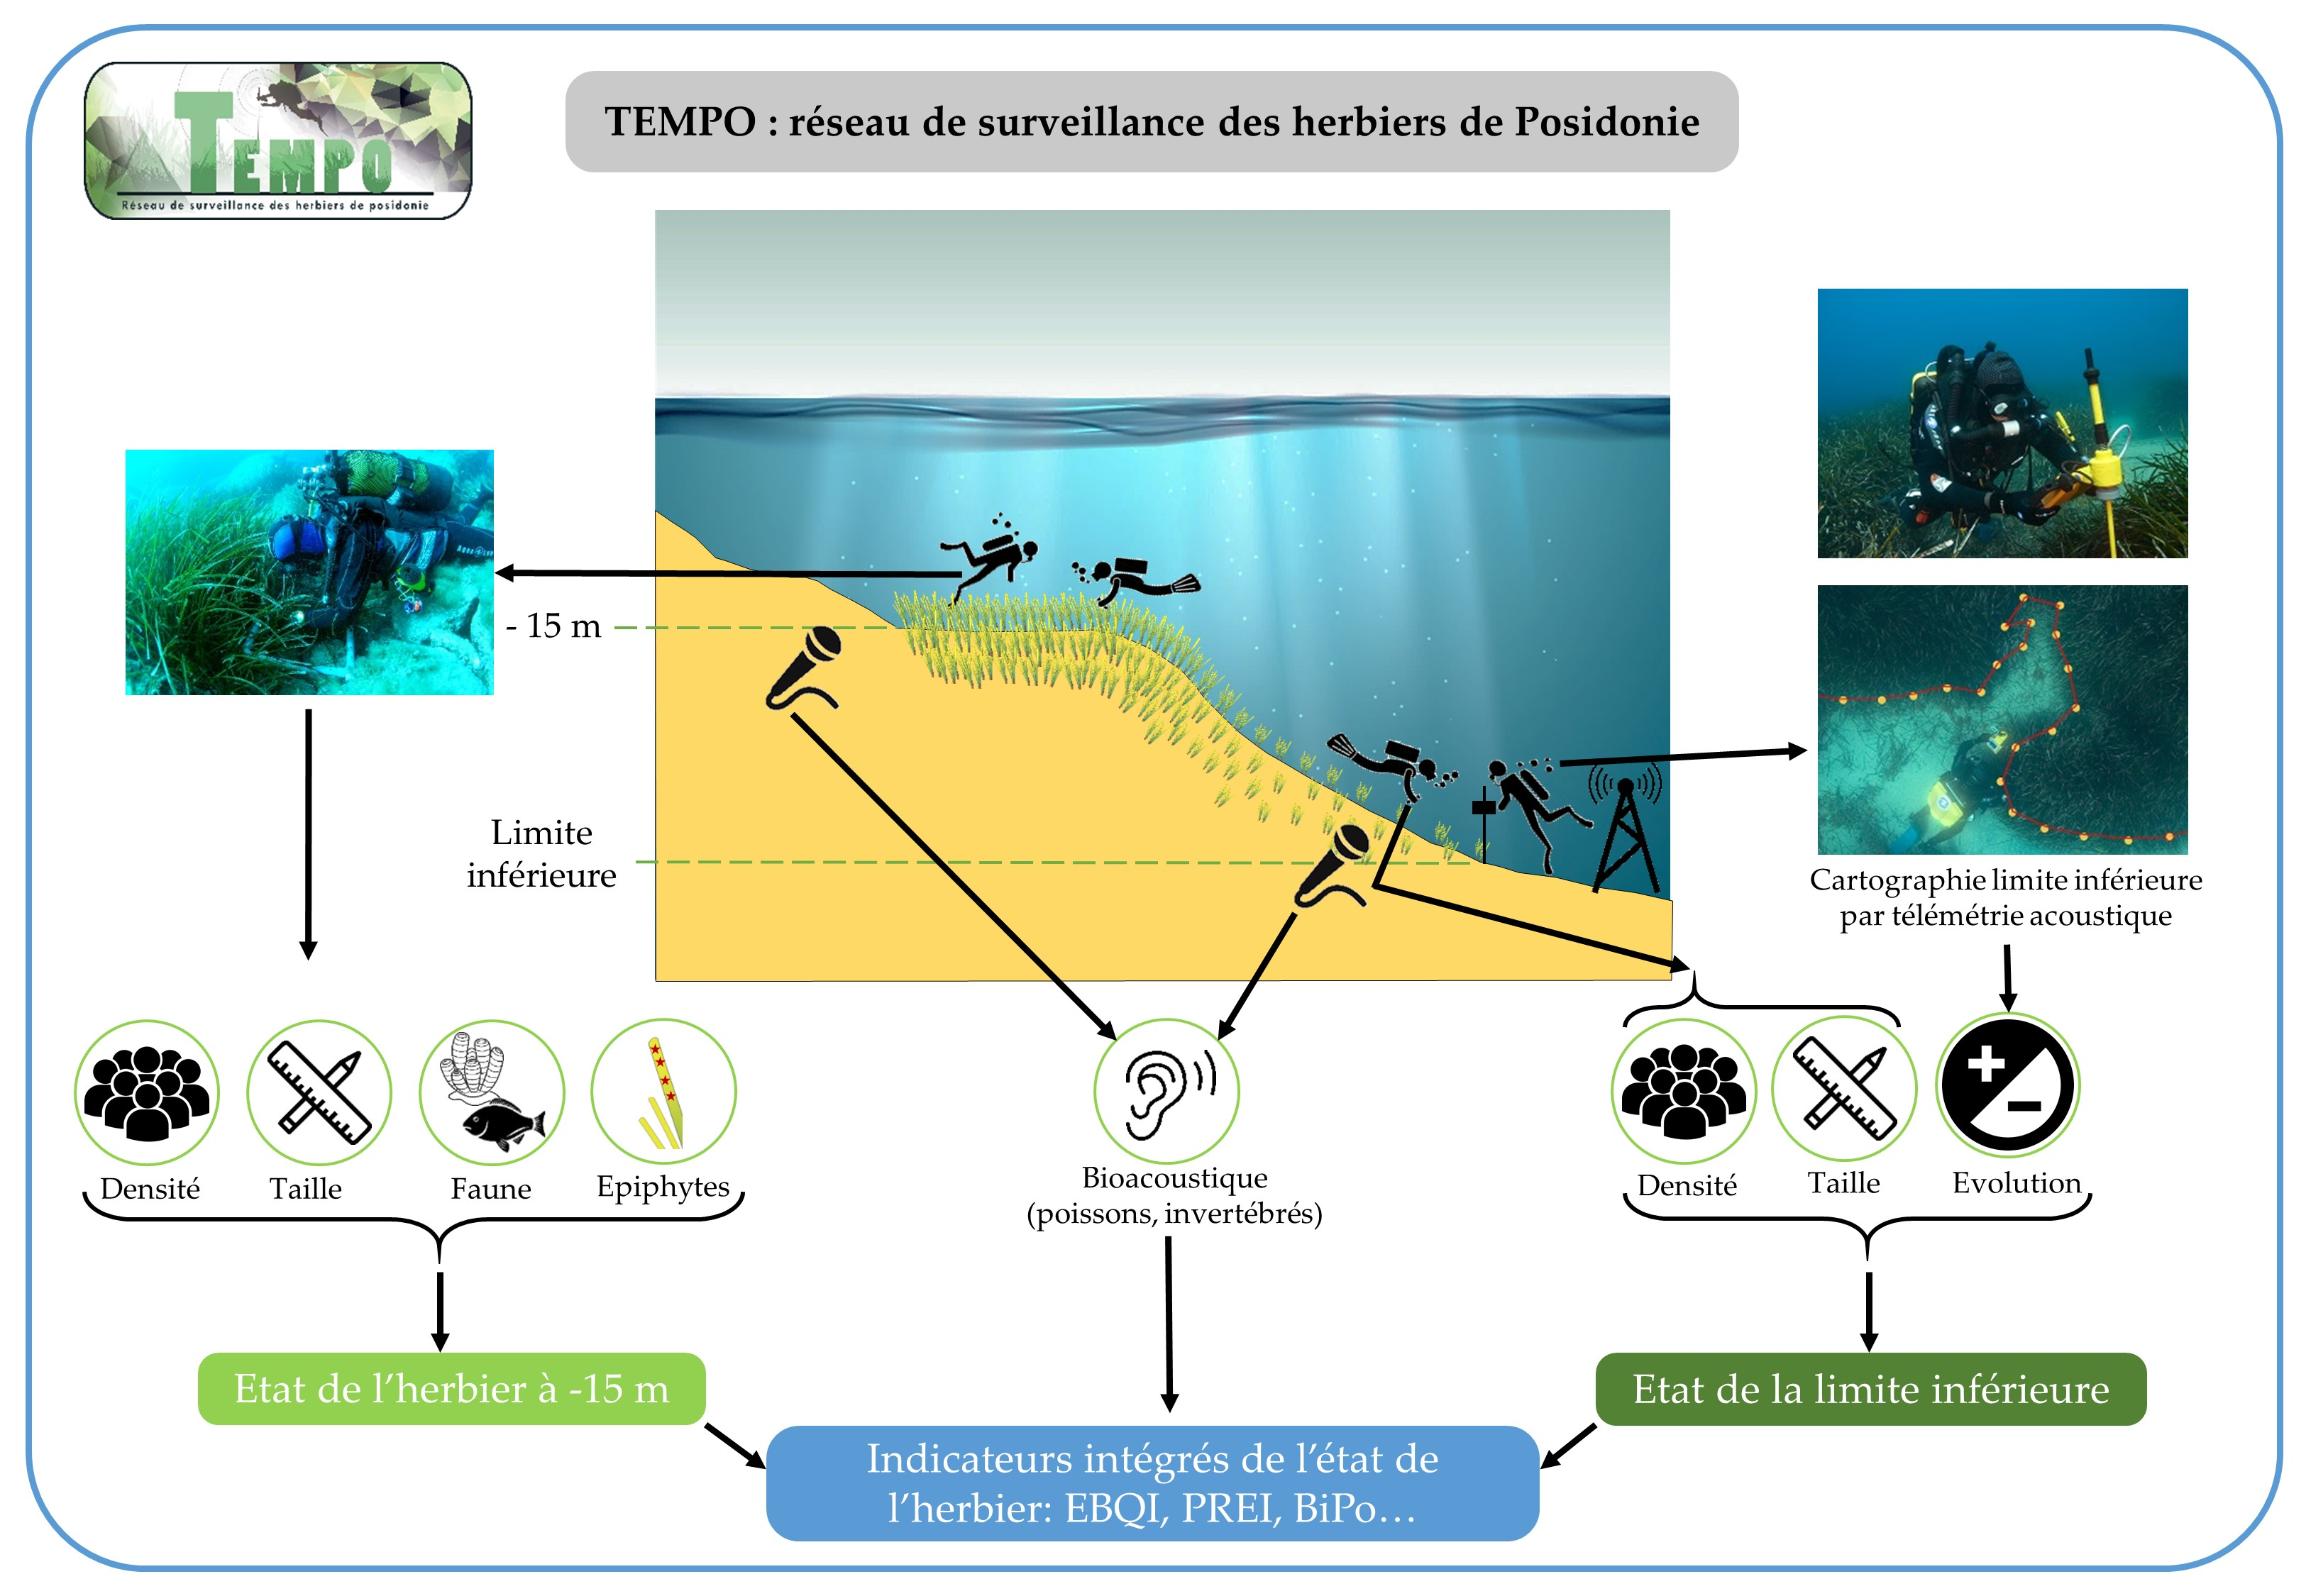
\includegraphics[width=\linewidth,keepaspectratio]{./1_intro/encart_TEMPO}
		\caption[TEMPO : réseau de surveillance des herbiers de posidonie en Méditerranée française]{TEMPO : réseau de surveillance des herbiers de posidonie en Méditerranée française.}
	\label{figure_intro17}
\end{center}
\end{figure}
\end{sidewaysfigure}

\newpage

\subsubsection{RECOR : un réseau de surveillance des assemblages des récifs coralligènes en Méditerranée française}\label{intro.2.3.3}

« Il est urgent de développer de nouvelles méthodes pour comprendre la structuration de ces assemblages [coralligènes], et évaluer les impacts auxquels ils sont soumis, afin de fournir un état de référence et explorer les possibles trajectoires d’évolution de ces assemblages d’une grande diversité » \citep{kipson_rapid_2011}. RECOR est un réseau de surveillance de l’état écologique des récifs coralligènes en Méditerranée, opéré par Andromède océanologie depuis 2010 avec le soutien de l’Agence de l’eau Rhône-Méditerranée-Corse. Comme pour TEMPO, la caractérisation de l’état écologique des récifs est réalisée par campagne régionale annuelle sur la période mi-mai / fin juin. Chaque année, une des trois régions concernées par cette agence de l’eau (Corse, région Sud-Provence-Alpes Côte d’Azur et Occitanie) est échantillonnée, avec un roulement sur trois ans. Toutes régions confondues, le réseau RECOR permet au total l’échantillonnage de 177 stations situées sur 97 sites (i.e. récifs) lors des trois années de suivi (\autoref{figure_intro18}). Les stations sont situées à des profondeurs comprises entre 17 et 90 m, et un site peut inclure plusieurs stations à des profondeurs différentes.

%%%%%%%%%%%%%%%%%%%%%%%%%%%%%%%%%%%%%%%
%%% Figure intro18: le réseau RECOR %%%
%%%%%%%%%%%%%%%%%%%%%%%%%%%%%%%%%%%%%%%
\begin{figure}[H]
	\begin{center}
	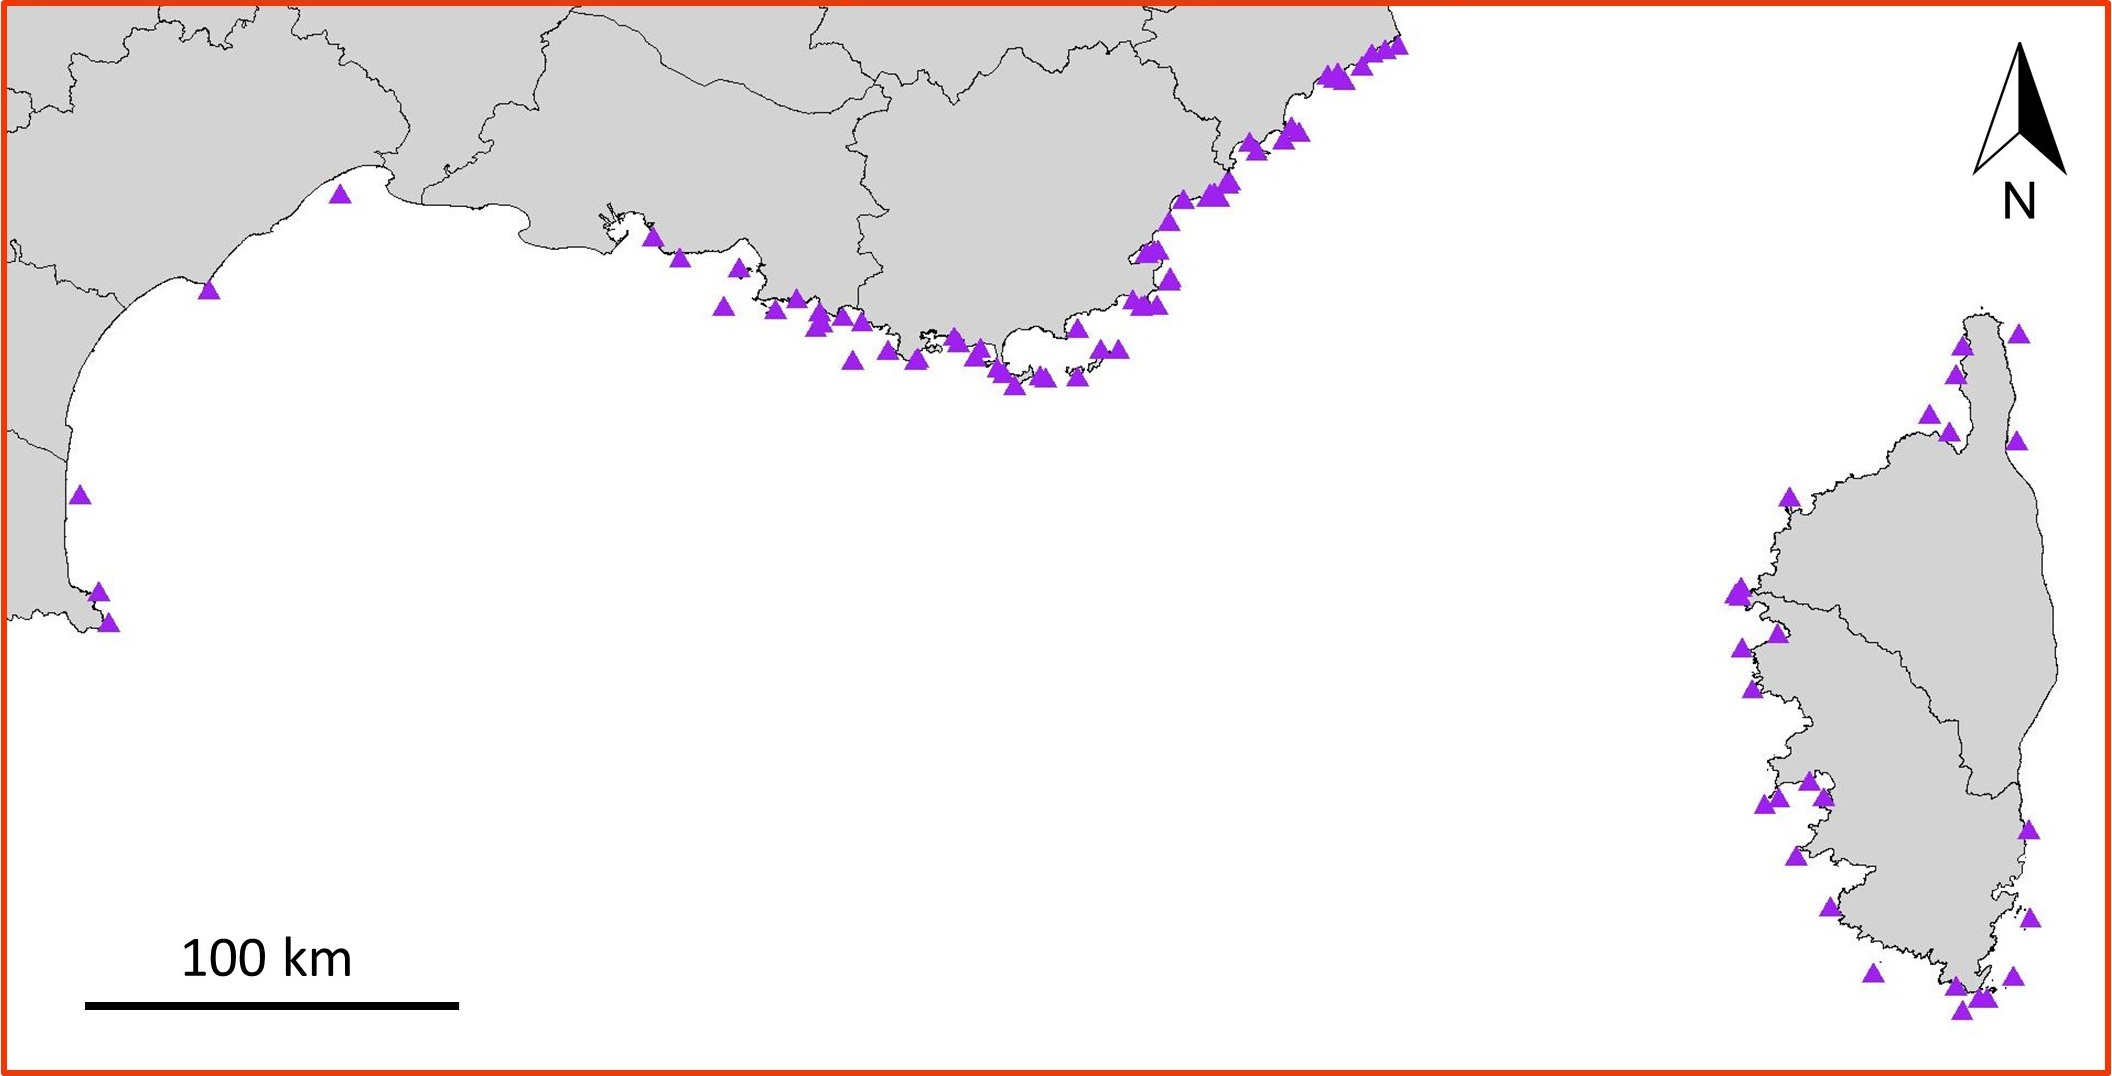
\includegraphics[width=\linewidth,keepaspectratio]{./1_intro/reseau_RECOR}
		\caption[Localisation des 97 sites du réseau de surveillance RECOR]{Localisation des 97 sites du réseau de surveillance RECOR.}
	\label{figure_intro18}
\end{center}
\end{figure}

Encore plus que pour les habitats peu profonds, le suivi des récifs coralligènes est limité par les contraintes physiologiques du plongeur. En effet, à ces profondeurs (couramment 50 à 80 m de fond), chaque minute de plongée supplémentaire nécessite un temps accru de décompression. Par conséquent, la méthode de suivi la plus utilisée est le quadrat photographique : le plongeur réalise 30 images standardisées (distance au récif et éclairage contrôlé), échantillonnées à différents endroits du récif, qui sont ensuite identifiées par un taxonomiste une fois de retour au bureau \citep{deter_rapid_2012}. Les images sont analysées à l’aide du logiciel Coral Point Count \citep{cpce_coral_2011} 4.1 « coralligenous assemblages version » en échantillonnant aléatoirement 64 points par image (soit 30 $\times$ 64 = 1920 points par station), et chaque point est identifié par le même expert taxonomiste. Celui-ci calcule ensuite, à l’échelle de la station, des indicateurs d’état de conservation et de diversité, notamment :

\begin{itemize}
    \item \textbf{Coralligenous Assemblage Index (CAI)} \citep{deter_preliminary_2012} : indicateur représentatif de l’état écologique d’un récif. Il prend en compte trois composantes : la proportion de bioconstructeurs, la proportion de vase et la proportion de bryozoaires. Chacune des trois valeurs est standardisée par la valeur minimale (pour la vase) ou maximale (pour les bioconstructeurs et les bryozoaires) mesurée par région. Il est calculé comme suit :
    
    \begin{equation}
        \text{CAI\textsubscript{i}}=\frac{1}{3}\times(\frac{1-sludge_i}{1-\min_{i}sludge_i}+\frac{majbuilders_i}{\max_{i}majbuilders_i}+\frac{bryozoans_i}{\max_{i}bryozoans_i})
        \label{eqintro.2}
    \end{equation}
    
    \item \textbf{Indice de Shannon} \citep{magurran_measuring_2004} : voir section \ref{intro.2.1}~;
    
    \item \textbf{Nécroses} : pourcentage de mortalité d’algues bioconstructrices (potentiellement lié à la température, pathogènes, pollution, compétition…)~;
    
    \item \textbf{Indice algues filamenteuses} : pourcentage d’algues filamenteuses qui prolifèrent et recouvrent les récifs (potentiellement lié à la température, nutriments et salinité).

\end{itemize}

Ces indicateurs permettent de définir un état de diversité et de conservation à un instant t, et le suivi de leur évolution dans le temps permet de quantifier la potentielle dégradation ou récupération des récifs. Conjointement à ces analyses, les plongeurs réalisent des mesures de tailles, densités et nécroses de gorgones au sein de 30 quadrats de 0,5 $\times$ 0,5 m (\autoref{figure_intro19}). Les gorgones sont des espèces érigées suspensivores sensibles aux perturbations mécaniques et aux variations de qualité de l’eau et de la température, et sont donc un bon témoin de la qualité écologique d’un récif. Enfin, comme pour le réseau TEMPO, des mesures bioacoustiques sont réalisées sur certains sites afin de quantifier l’activité des espèces mobiles (en partenariat avec l’équipe Chorus (\href{https://chorusacoustics.com/}{https://chorusacoustics.com/}) qui porte le réseau de surveillance CALME).

\medskip

\setlength{\fboxsep}{5pt}
\setlength{\fboxrule}{0.6pt}
\noindent\framebox{%
  \begin{minipage}{\linewidth}
    Le protocole RECOR permet d’acquérir en peu de temps une \textbf{grande quantité de données} indispensables à \textbf{l’évaluation de la diversité des assemblages coralligènes} et de leur \textbf{état de santé}. Cependant, l’analyse a posteriori des images pour \textbf{l’identification des espèces du coralligène} requiert des \textbf{compétences taxonomistes} et sont extrêmement \textbf{chronophage} (1 920 identifications par station sont nécessaires à l’évaluation de ces assemblages complexes).
  \end{minipage}
}

%%%%%%%%%%%%%%%%%%%%%%%%%%%%%%%%%%%%%%%%
%%% Figure intro19: la méthode RECOR %%%
%%%%%%%%%%%%%%%%%%%%%%%%%%%%%%%%%%%%%%%%
\begin{sidewaysfigure}
\begin{figure}[H]
	\begin{center}
	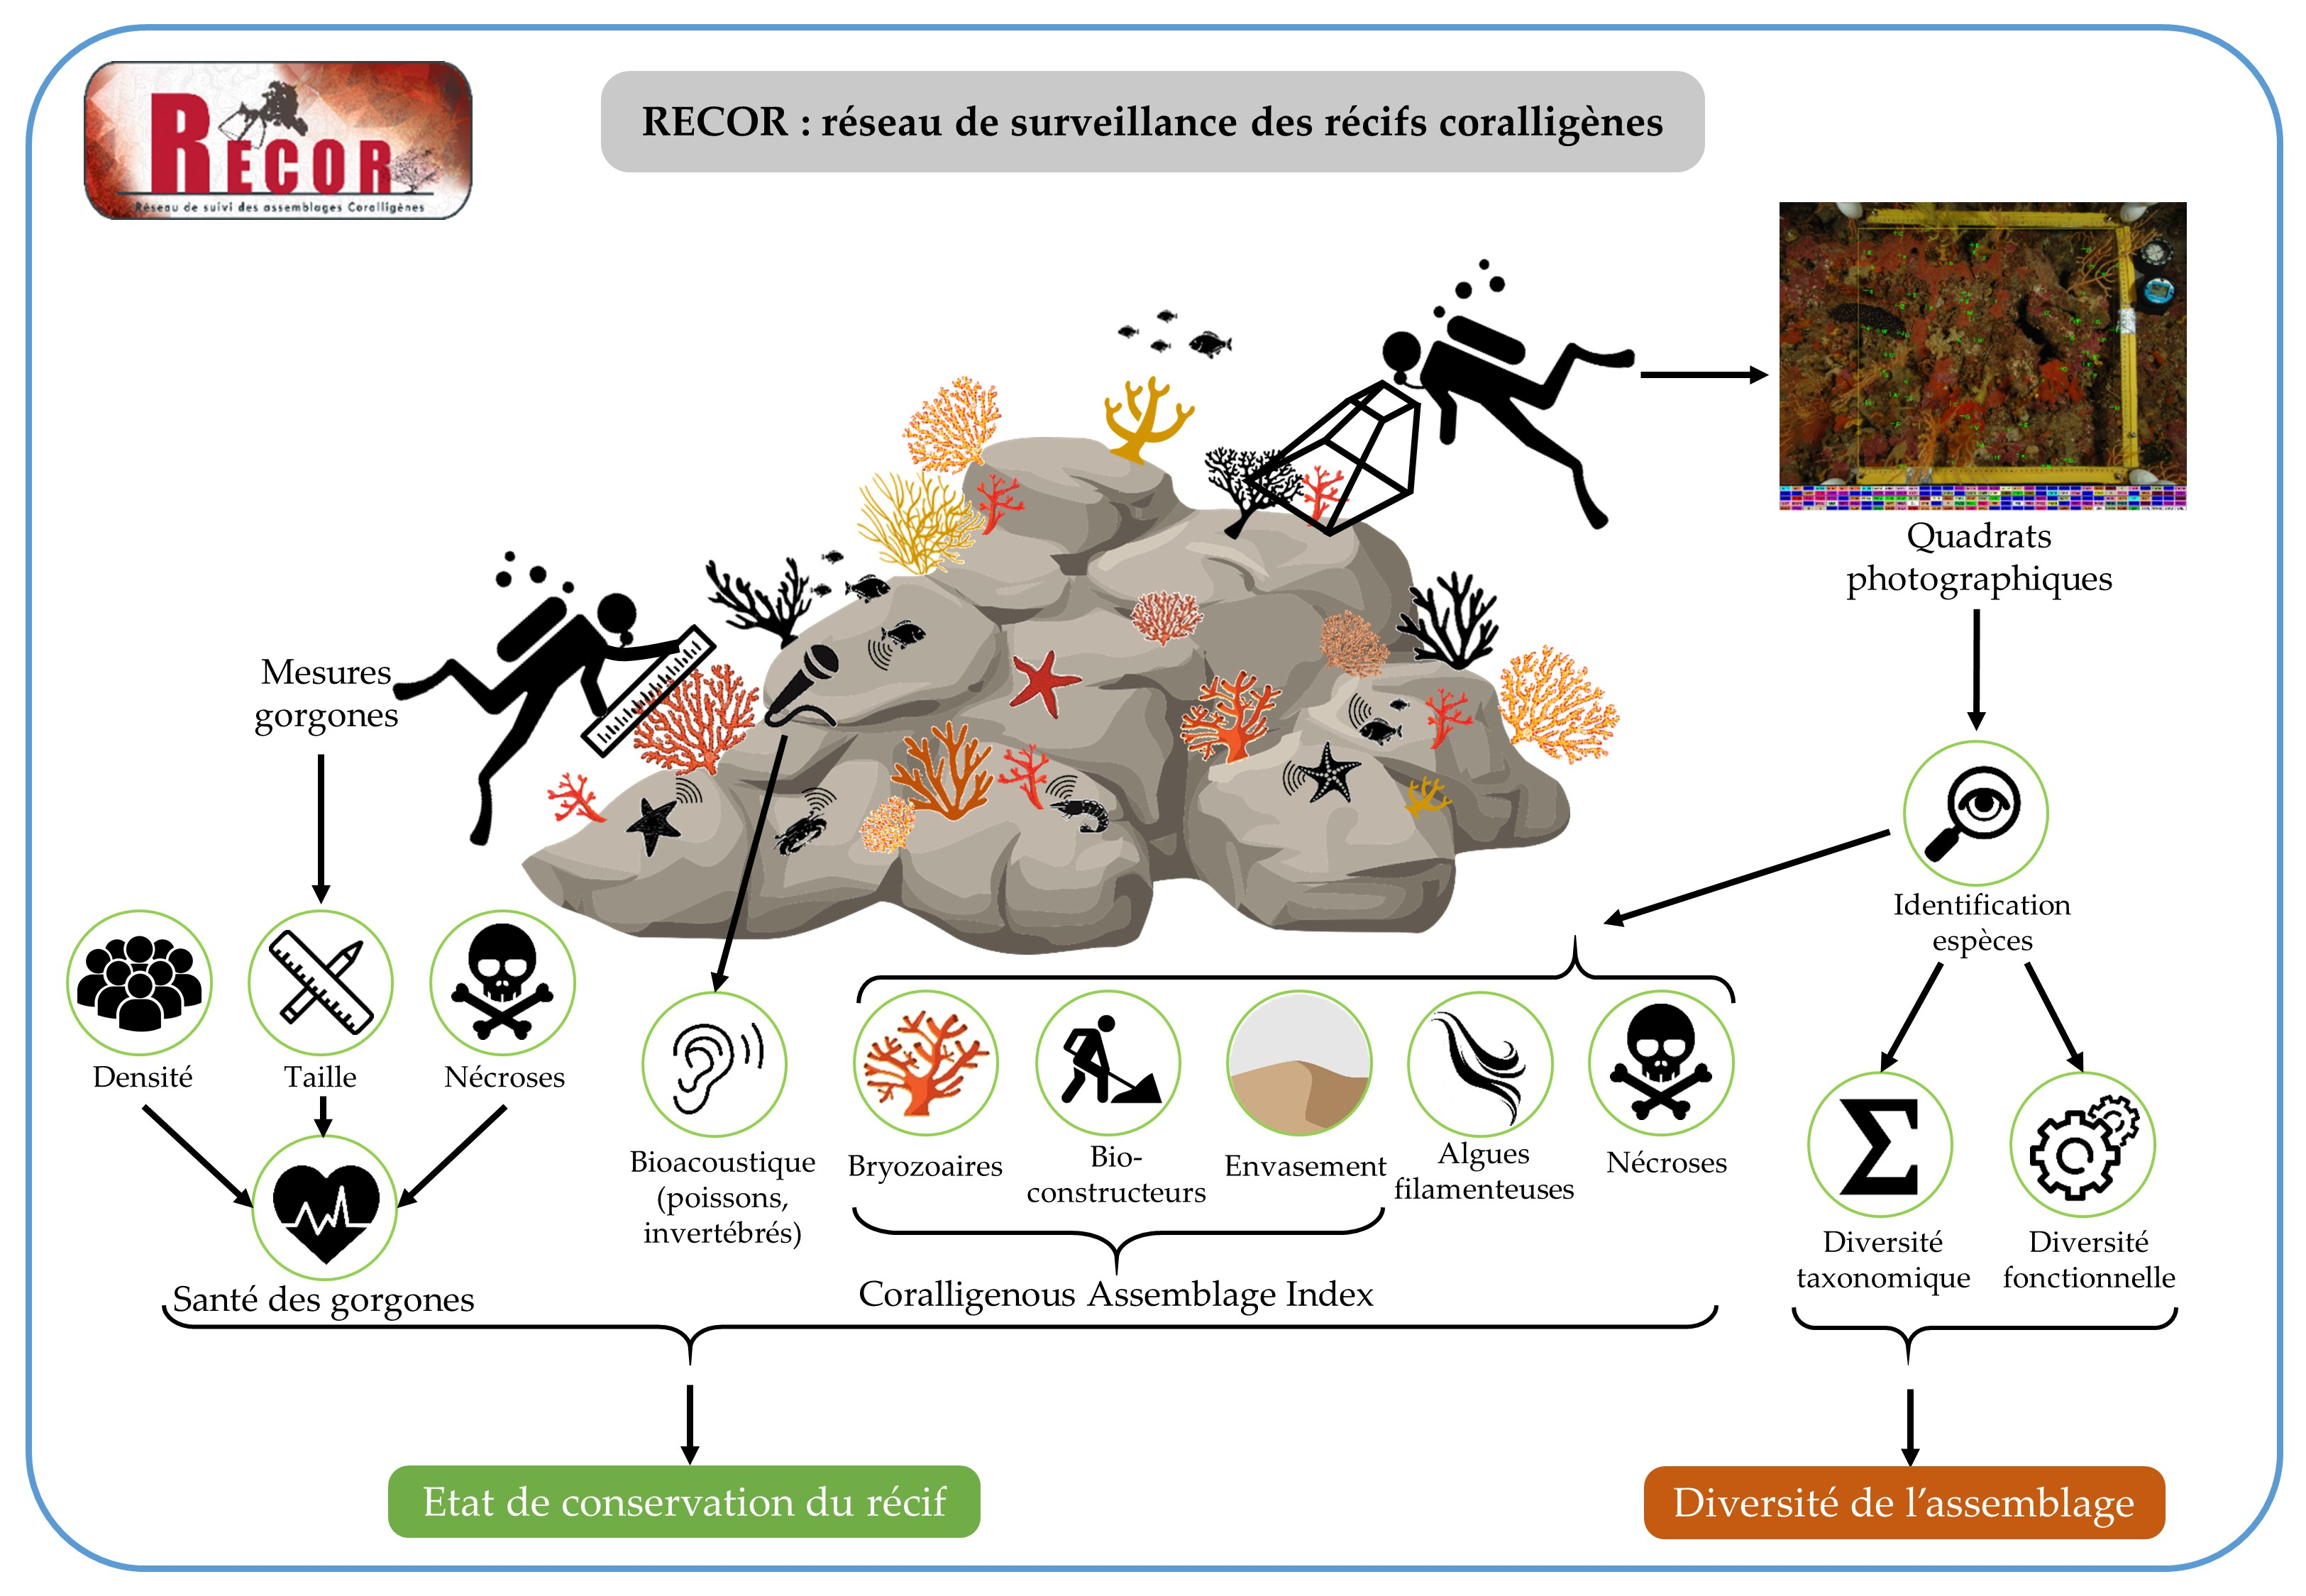
\includegraphics[width=\linewidth,keepaspectratio]{./1_intro/encart_RECOR}
		\caption[RECOR : réseau de surveillance des récifs coralligènes en Méditerranée française]{RECOR : réseau de surveillance des récifs coralligènes en Méditerranée française.}
	\label{figure_intro19}
\end{center}
\end{figure}
\end{sidewaysfigure}

\newpage

%%% PROBLEMATIQUE %%%
\section{Problématique et objectifs de la thèse}\label{intro.3}

La \textbf{biodiversité mondiale} subit actuellement d’importantes \textbf{pressions d’origine anthropique}, menant à un rythme d’extinction d’espèces et de dégradation des habitats sans précédent depuis la dernière grande extinction de masse il y a 66 millions d’années. Les \textbf{écosystèmes marins}, en particulier, qui concentrent une grande partie de la \textbf{biodiversité} et des \textbf{services écosystémiques}, souffrent du cumul de ces pressions à l’échelle globale. La mise en place de \textbf{mesures de conservation efficaces} pour limiter les impacts anthropiques sur le milieu marin est cruciale, particulièrement en \textbf{Méditerranée}, une mer qui concentre à la fois de hauts niveaux de biodiversité et d’importantes pressions cumulées. Cependant, les \textbf{difficultés d’accès} au monde sous-marin limitent considérablement l’acquisition de données et donc les connaissances sur la distribution et l’évolution de sa biodiversité. La \textbf{surveillance écologique} de ces habitats sensibles est primordiale : elle doit permettre aux décideurs et gestionnaires d’établir des \textbf{mesures de conservation} et de quantifier leur efficacité afin de limiter au maximum les impacts anthropiques sur ces habitats. C’est l’objet des deux réseaux de surveillance \textbf{TEMPO} et \textbf{RECOR}, centrés sur les \textbf{herbiers de posidonie} et les \textbf{récifs coralligènes}, les deux habitats les plus riches de Méditerranée. S’ils bénéficient d’une dizaine d’années d’expérience, ces deux réseaux sont en constante évolution. Les développements récents en matière d’analyses d’images offrent des opportunités intéressantes pour alimenter la chaîne d’\textbf{acquisition} et de \textbf{traitement} de données écologiques. Les potentialités sont une réduction des incertitudes, l’augmentation de la couverture spatiale et temporelle, et la diminution de temps de traitement par l’automatisation de traitements.

La \textbf{reconnaissance d’images} a connu une grande révolution avec le développement des premiers grands \textbf{réseaux de neurones convolutifs} au début des années 2010. Ces algorithmes, dont les performances dépassent parfois même celles d’un opérateur humain, sont de plus en plus utilisés en sciences, notamment en écologie avec la \textbf{reconnaissance d’espèces}. Dans le même temps, un autre type de traitement d’images s’est largement développé grâce à l’amélioration des algorithmes et à l’explosion de la puissance de calcul : la \textbf{photogrammétrie}. Cette technique permet de \textbf{reconstruire en trois dimensions} un objet à partir d’images en deux dimensions réalisées sous différents angles de vue. Comme les réseaux de neurones convolutifs, elle connaît des applications de plus en plus variées, y compris en écologie, car elle permet de capturer la \textbf{structure tridimensionnelle de l’habitat} et de reconstituer des images aériennes de très haute définition.

\textbf{L’objectif de cette thèse} est de répondre aux \textbf{besoins de la surveillance} des habitats marins par le développement de méthodes et d’indicateurs innovants. Plus particulièrement, cette thèse CIFRE (Convention Industrielle de Formation par la REcherche) vise à répondre aux besoins des réseaux de surveillance TEMPO et RECOR, portés par la société Andromède Océanologie, par le \textbf{développement de méthodes opérationnelles} d’évaluation de la santé des herbiers de posidonie et des récifs coralligènes basées sur les réseaux de neurones convolutifs et la photogrammétrie. 

En effet, le réseau RECOR se base en partie sur de très nombreuses identifications d’espèces du coralligène par un expert taxonomiste, tâche chronophage et principale limite à la capacité d’échantillonnage. En bénéficiant de la \textbf{grande base d’images annotées} constituée au cours des années, \textbf{l’entraînement d’un réseau de neurones convolutifs} permettrait d’automatiser l’interprétation des images collectées et d’augmenter de fait le volume de données potentiellement analysables. Par ailleurs, les récifs coralligènes possèdent une \textbf{structure tridimensionnelle} complexe, encore très peu étudiée et qui n’est aujourd’hui pas prise en compte par le réseau RECOR, or elle est le reflet de la longue évolution de ces récifs biogéniques et pourrait entretenir des liens étroits avec la \textbf{composition des assemblages}. La \textbf{photogrammétrie} apparaît comme une technique de choix pour étudier ces liens, car elle permet de reconstruire en trois dimensions les récifs dans toute leur complexité et d’\textbf{analyser leur structure} dans le détail avec des indicateurs architecturaux. Enfin, la cartographie de la limite inférieure des herbiers de posidonie souffre d’un manque de précision et d’un temps d’acquisition physiologiquement contraignant pour le plongeur avec la télémétrie acoustique. La \textbf{photogrammétrie} pourrait offrir des solutions de \textbf{cartographie rapide et automatisée} de cette limite, permettant d’améliorer l’efficacité et la précision des suivis réalisés dans le cadre du réseau TEMPO. 

La partie suivante du manuscrit détaille les aspects méthodologiques concernant les deux méthodes d’analyses d’images employées dans le cadre de ces travaux de recherche (i.e. réseaux de neurones convolutifs et photogrammétrie), afin de fournir au lecteur les bases théoriques à la bonne compréhension du reste du manuscrit. Le travail de recherche à proprement parler se divise en quatre chapitres détaillant successivement le développement et l’application des méthodes opérationnelles basées sur ces deux techniques d’analyse d’images, avec les objectifs scientifiques suivants :

\begin{enumerate}
    \item Développer et entraîner un réseau de neurones convolutifs à reconnaître les espèces du coralligène avec un taux d’erreur semblable ou inférieur à celui d’un expert taxonomiste  (\textbf{\autoref{chapitre1-deep}})~;
    
    \item Définir un protocole d’acquisition plongeur pour réaliser des reconstructions 3D d’habitats marins par photogrammétrie, et quantifier la précision et la résolution de ces reconstructions  (\textbf{\autoref{chapitre2-methode}})~;
    
    \item Développer une méthode de microcartographie automatique des herbiers de posidonie basée sur la photogrammétrie pour permettre un suivi à fine échelle et rapide de la limite inférieure des herbiers  (\textbf{\autoref{chapitre3-herbiers}})~;
    
    \item Caractériser la structure des récifs coralligènes par photogrammétrie et explorer les liens entre structure, composition des assemblages et conditions environnementales (\textbf{\autoref{chapitre4-structure}}).
    
\end{enumerate}

Enfin, la dernière partie de ce manuscrit est consacrée à la synthèse et la discussion de l’ensemble des résultats de ce travail de thèse. Cette partie détaillera également comment les principales avancées peuvent être intégrées aux réseaux de surveillance TEMPO et RECOR, et ouvrira sur les perspectives de recherches à l’issue de ce travail.

%%% Méthodes
\part{Méthodes}
\pagestyle{preambule}
%\chapter{Introduction générale} \label{Introduction générale}
\setcounter{section}{0} % 
\renewcommand*{\theHsection}{chY.\the\value{section}}
% COVER PAGE
\centerline{\bfseries\textcolor{bleusection}{ \Huge Méthodes}}  

\bigskip

% Figure cover
\begin{tikzpicture}
  \def\ig{%
   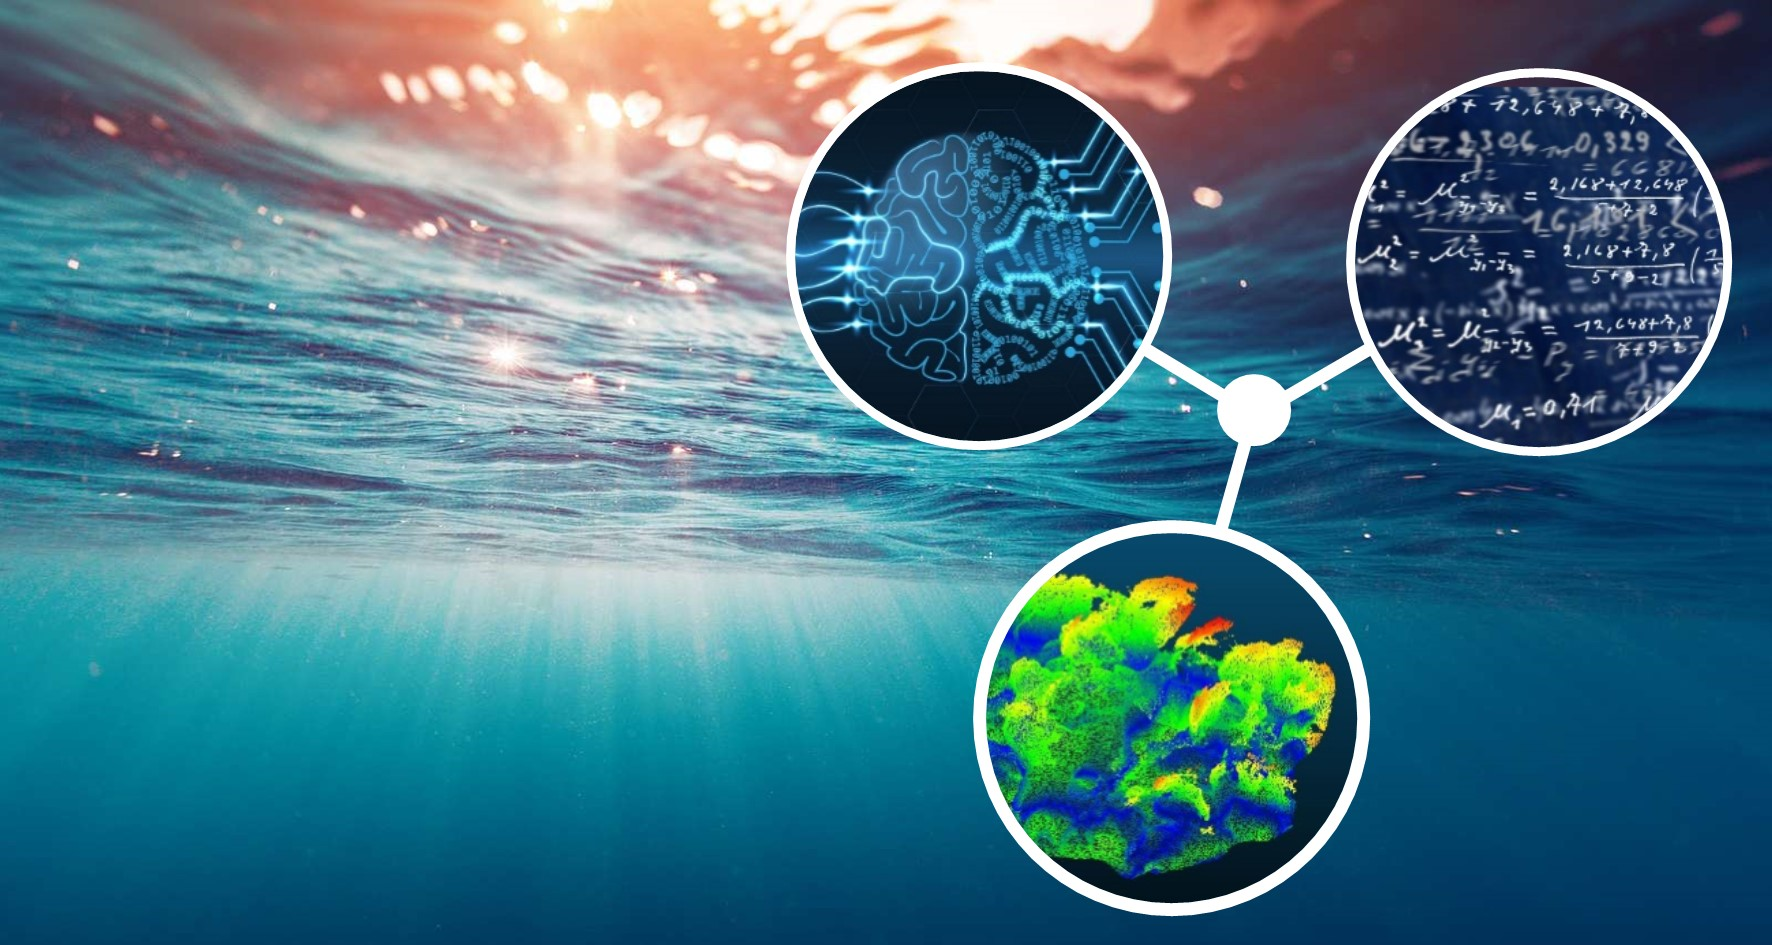
\includegraphics[width=\linewidth,keepaspectratio]{./2_methodes/cover_methodes}}
 \node [inner sep=0pt](mypicture) at (0,0) {\phantom{\ig}};
 \clip[rounded corners=5mm] ($(mypicture.south west)+(\bord,\bord)$) rectangle ($(mypicture.north east)-(\bord,\bord)$);
 \node[inner sep=0pt](mypicture) at (0,0) {\ig};
\end{tikzpicture}

% Table des matières méthodes
{\LARGE
\begin{enumerate}[label=\textcolor{bleusection}{\arabic*}{.}, leftmargin=2cm]
  \item \nameref{methodes.1}
  \item \nameref{methodes.2}
\end{enumerate}
}

% DEBUT METHOGOLOGIE
\clearpage
\pagestyle{methodo}

\section{Analyses d'images par apprentissage profond}\label{methodes.1}

L’analyse d’images est un champ de recherche très actif, qui a pour but d’interpréter automatiquement le contenu d’une image afin d’y détecter un objet (i.e. détection), de segmenter l’image en zones de même nature (i.e. segmentation), de reconnaître des objets (i.e. classification), ou encore de mesurer une variable continue à partir de la structure de l’image (i.e. régression). L’analyse d’images a connu d’importants rebondissements depuis une dizaine d’années, grâce à l’explosion de la puissance de calcul (notamment l’utilisation des cartes graphiques, ou « Graphical Processing Unit » (GPU)) et à l’apparition de nouveaux algorithmes : les Réseaux de Neurones Convolutifs (RNC). Nous détaillerons dans cette section l’utilisation des RNC à des fins de classification d’images.

\subsection{Structure des réseaux de neurones convolutifs}

Comme leur nom le laisse deviner, les RNC sont cousins des réseaux de neurones, ou « perceptron multicouche », imaginés dans les années 1970 et mis au point par David Rumelhart \citep{rumelhart_learning_1986}. Ces algorithmes visent à simuler les mécanismes d’apprentissage des êtres vivants en reproduisant le fonctionnement d’un système nerveux : de nombreuses unités, les « neurones », sont interconnectées et réagissent à un stimulus en émettant un signal qui parcourt le réseau et produit une réaction ou une interprétation \citep{aggarwal_neural_2018}. L’intensité des signaux entre les différents neurones s’adapte à mesure que l’être vivant est confronté à différentes situations ou stimuli, afin de peu à peu améliorer la réaction ou la capacité de jugement : c’est le phénomène d’apprentissage.

Les RNC sont des réseaux à propagation directe (« feedforward ») qui incluent des couches de convolutions permettant de prétraiter l’information avant qu’elle ne soit analysée par le perceptron multicouche. Les convolutions permettent notamment de réduire significativement le nombre de paramètres pour les grandes images, car dans le cas d’un perceptron multicouche avec un neurone associé à chaque pixel dans la couche d’entrée, le nombre de paramètres augmente exponentiellement avec la taille de l’image. Par ailleurs, les RNC permettent de faire ce que l’on appelle un « apprentissage de bout en bout » (pour « end-to-end learning ») : les couches de convolutions apprennent à extraire les variables les plus pertinentes pour la classification, qu’un perceptron multicouche apprend à interpréter pour produire sa classification (\autoref{figure_methodo1}). Ces architectures contiennent souvent un grand nombre de couches à entraîner, c’est pour quoi il est question « d’apprentissage profond » (ou « deep learning »).

L’idée des convolutions est inspirée d’une étude portant sur le fonctionnement du cortex visuel du chat \citep{hubel_receptive_1959}, qui a montré que certaines régions de son champ de vision semblent exciter spécifiquement certains neurones. La première architecture basique inspirée de cette observation est le Neocognitron \citep{fukushima_neocognitron_1988}, généralisée quelques années plus tard par le travail de LeCun et al. (1998) avec le LeNet-5 capable de reconnaître des chiffres écrits à la main en niveaux de gris. Les RNC ont depuis connu un développement important, notamment 

%%%%%%%%%%%%%%%%%%%%%%%%%%%%%%%%%%%%%%%
%%% Figure methodo1: Structure CNNs %%%
%%%%%%%%%%%%%%%%%%%%%%%%%%%%%%%%%%%%%%%
\begin{sidewaysfigure}
%\enlargethispage{.5cm}
\begin{figure}[H]
	\begin{center}
	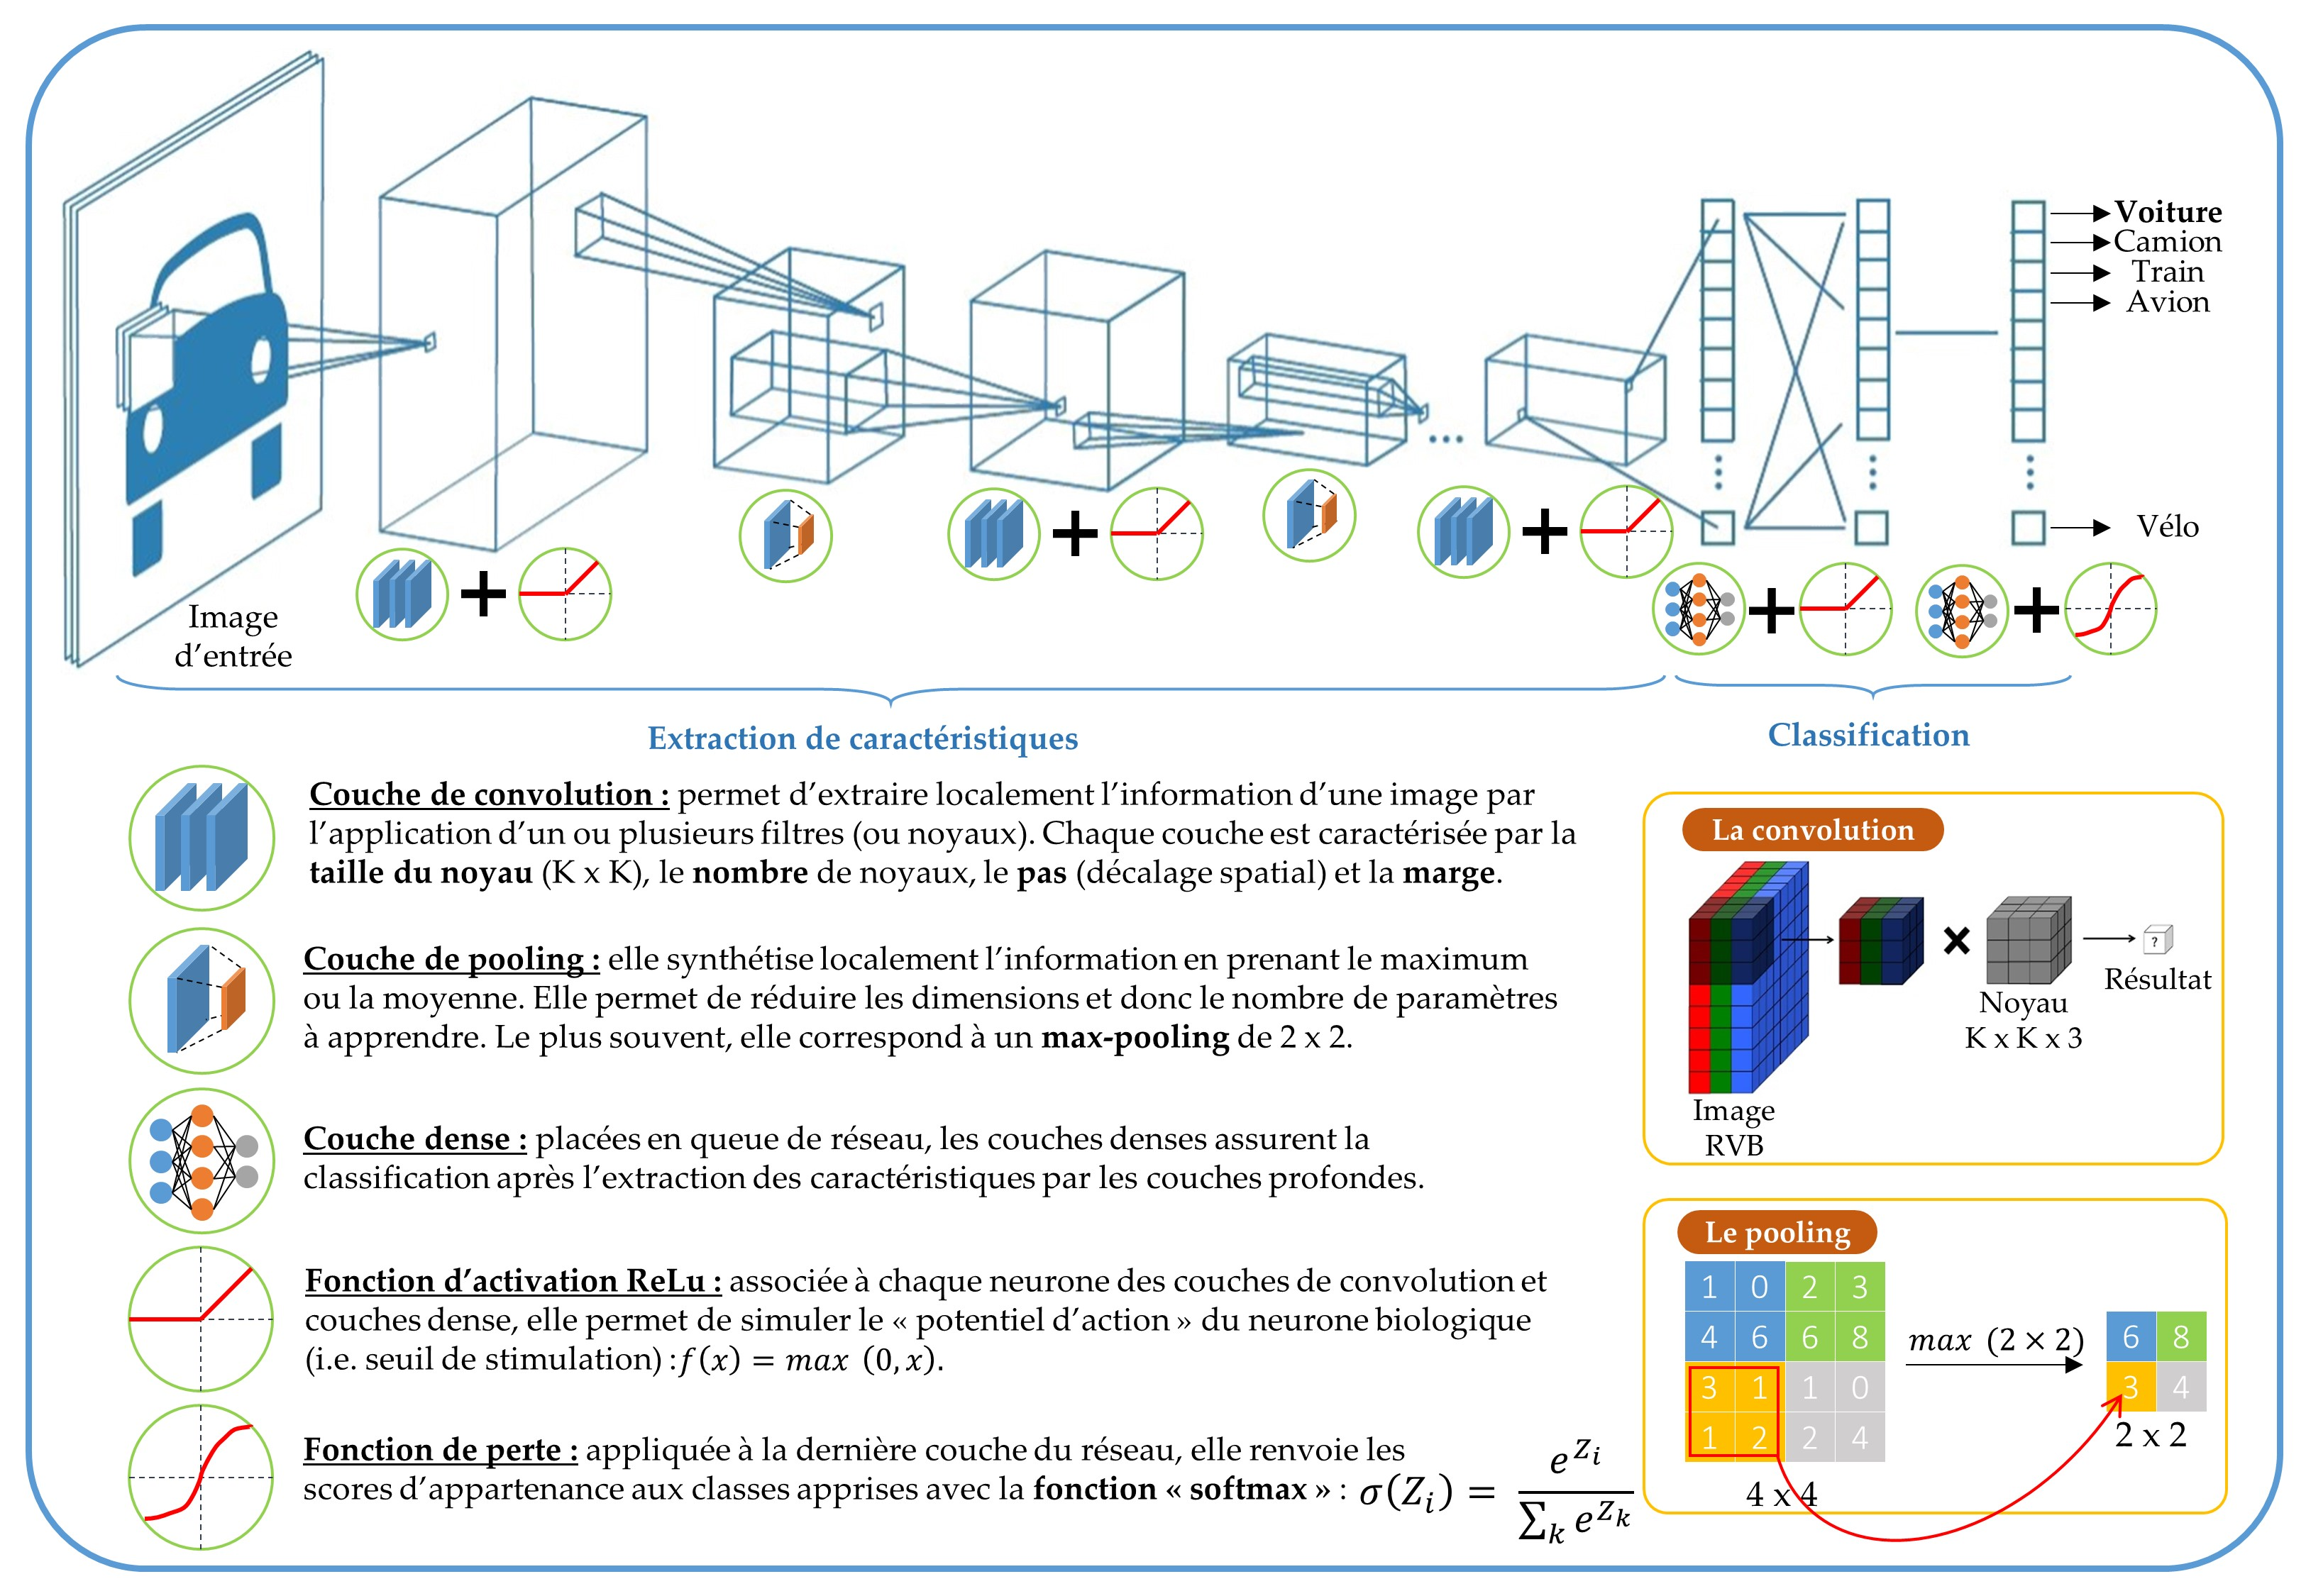
\includegraphics[width=\linewidth,keepaspectratio]{./2_methodes/encart_architecture}
		\caption[Vision schématique de l’architecture d’un réseau de neurones convolutifs destiné à la classification d’images]{Vision schématique de l’architecture d’un réseau de neurones convolutifs destiné à la classification d’images (schéma du réseau adapté de mathworks.com).}
	\label{figure_methodo1}
\end{center}
\end{figure}
\end{sidewaysfigure}

\noindent grâce à l’apparition de grosses bases de données annotées telles qu’ImageNet \citep{deng_imagenet:_2009} et l’augmentation de la puissance de calcul par l’utilisation des cartes graphiques. S’il existe aujourd’hui de nombreuses architectures, chacune ayant apporté sa pierre à l’édifice à un moment donné, les briques élémentaires des RNC sont toujours les mêmes : les couches de convolution, les couches de pooling et les couches denses \citep{lecun_deep_2015} (\autoref{figure_methodo1}).

\subsubsection{Les couches de convolution}

Une convolution permet d’extraire localement l’information d’une image à l’aide d’un filtre mobile, appelé « noyau de convolution », et produire une nouvelle image. Chaque pixel de l’image produite correspond à la combinaison linéaire des valeurs des pixels voisins de l’image d’entrée, dont les coefficients (« poids ») correspondent aux valeurs définies dans le noyau. Pour bien comprendre ce concept, il est important de souligner qu’une image peut posséder plusieurs canaux de couleurs, et donc elle doit être vue comme un volume (hauteur × largeur × canaux de couleurs). Par exemple, une image Rouge-Vert-Bleu (RVB) de 32 $\times$ 32 pixels sera représentée par un volume de 32 $\times$ 32 $\times$ 3, chaque tranche correspondant à un canal de couleur. Une convolution correspond dans ce cas à l’application d’un noyau à trois dimensions, glissant sur toute la hauteur et la largeur de l’image, en incluant tous les canaux de l’image (voir encart « La convolution », \autoref{figure_methodo1}), pour produire une image à deux dimensions (profondeur de 1). Dans le cas d’une image en dégradé de gris, à un seul canal, le noyau est donc de dimensions largeur $\times$ hauteur $\times$ 1. Le noyau est invariant en fonction des dimensions spatiales de l’image, i.e. les poids sont constants tandis que le noyau glisse sur l’ensemble de l’image. Cette propriété rend une convolution indépendante d’une translation de la donnée d’entrée. Généralement, une couche de convolution est constituée de plusieurs noyaux afin d’extraire différentes informations de l’image d’entrée.

Les quatre hyperparamètres d’une couche de convolution sont :

\begin{itemize}
    \item \textbf{La taille du noyau (« kernel size ») :} largeur $\times$ hauteur du filtre, en pixels (la profondeur est toujours égale au nombre de canaux de l’image en entrée). La taille du noyau définit le niveau d’information extraite : plus elle est petite, plus le noyau extrait une information locale~;
    
    \item \textbf{Le nombre de filtres :} nombre de noyaux utilisés dans la couche. Les poids de chaque noyau sont appris par le réseau afin d’extraire les prédicteurs les plus pertinents au vu de la tâche de classification. Le nombre de noyaux permet de contrôler le volume de sortie et de gérer la dimensionnalité dans le réseau ;
    
    \item \textbf{Le pas (« stride ») :} décalage spatial entre deux applications du noyau sur l’image, en pixels. Un pas de un fera glisser le noyau d’un pixel par un pixel sur l’image en entrée, et produira ainsi une image en sortie de même dimension spatiale. Plus le pas est grand, plus la dimension spatiale de l’image de sortie sera petite ;
    
    \item \textbf{La marge (« padding ») :} l’application du noyau pose un problème lorsque l’on se trouve sur les bordures de l’image, où il est impossible de réaliser les calculs pour ces pixels. Sans ajout d’une marge à l’image d’entrée, la convolution produit donc une image de plus petites dimensions spatiales. Afin de conserver les dimensions, il est courant d’ajouter une marge à l’image d’entrée (de largeur ($K$ – 1) / 2 si $K$ est la largeur du noyau), généralement remplie de zéros \citep{aggarwal_neural_2018}.
    
\end{itemize}

\subsubsection{Les couches de pooling}

L’opération de « pooling » (ou « mise en commun ») (voir encart « Le pooling », \autoref{figure_methodo1}) est utilisée pour réduire la dimension des couches de convolution, elle est généralement placée entre des blocs de convolutions. Elle permet de réduire le nombre de paramètres à apprendre, et donc diminue les temps de calcul et permet d’éviter le phénomène de surapprentissage (« overfitting »). La couche de pooling opère indépendamment sur chaque partie du bloc de convolution en entrée (sur toute sa profondeur, il s’agit donc d’un volume) qu’elle réduit en utilisant une fenêtre mobile, ce qui augmente l’invariance du réseau à de petites transformations géométriques. Elle ne possède que deux hyperparamètres : la \textbf{taille} de la fenêtre et le \textbf{pas} (la fonction est déterminée, généralement la moyenne ou le maximum). La plupart du temps, la couche de pooling calcule la valeur maximale et utilise un pas et une taille de fenêtre égaux à 2. 

\subsubsection{Les couches denses}

Après l’extraction des prédicteurs par les couches de convolution et de pooling, la classification est assurée par un perceptron multicouche qui prend en entrée le résultat de la dernière couche de convolution, et produit en sortie le résultat de la classification. Ce perceptron multicouche est composé de plusieurs « couches denses » (ou « couches entièrement connectées ») : une « couche d’entrée », une ou plusieurs « couches cachées » et une « couche de perte » (c’est elle qui produit le vecteur de scores d’appartenance aux différentes classes). Dans une couche dense, les neurones artificiels ont des connexions avec toutes les sorties de la couche précédente (\autoref{figure_methodo2}).

%%%%%%%%%%%%%%%%%%%%%%%%%%%%%%%%%%%%%%%%%%%
%%% Figure methodo2: Les couches denses %%%
%%%%%%%%%%%%%%%%%%%%%%%%%%%%%%%%%%%%%%%%%%%
\begin{figure}[H]
	\begin{center}
	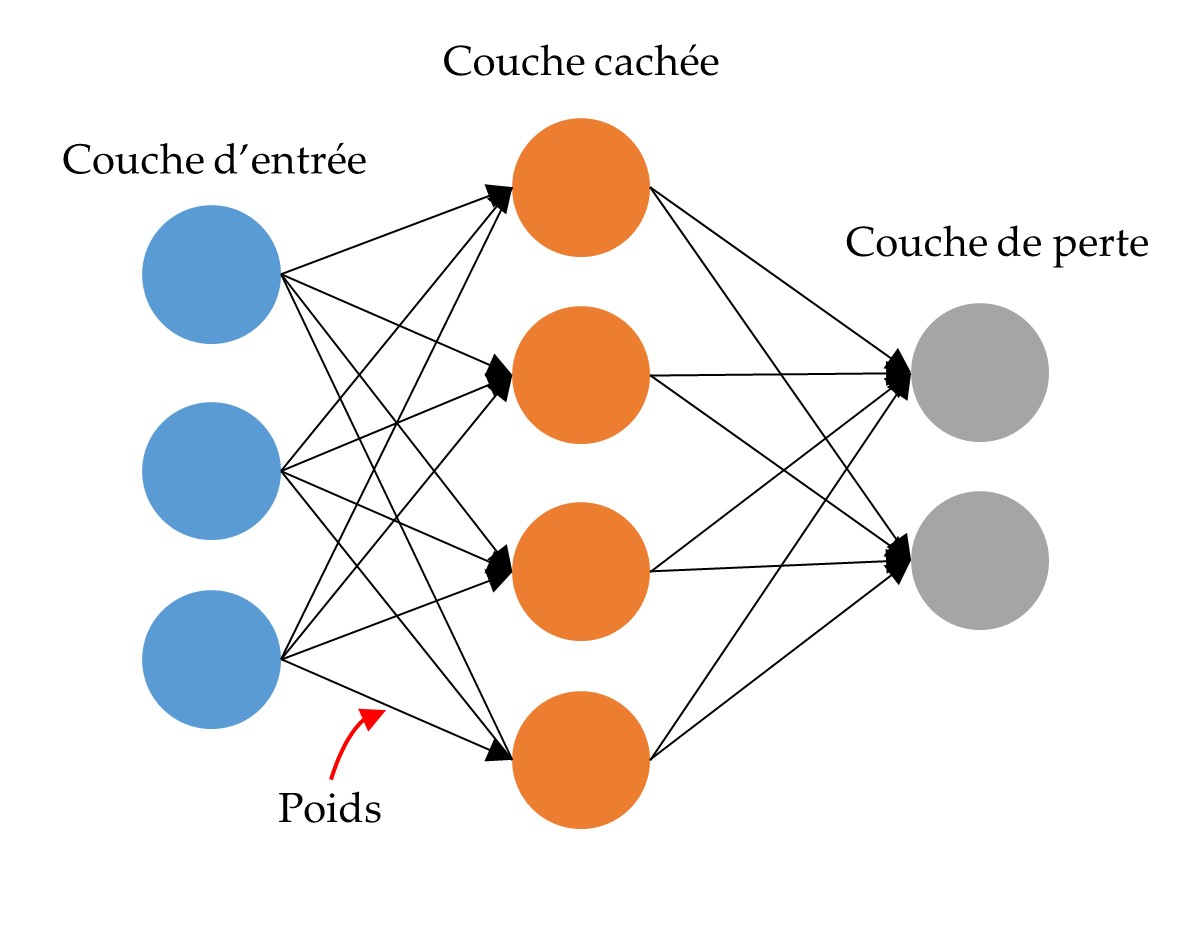
\includegraphics[width=0.7\linewidth,keepaspectratio]{./2_methodes/MLP}
		\caption[Fonctionnement schématique d’un perceptron multicouche en sortie d’un réseau de neurones convolutifs]{Fonctionnement schématique d’un perceptron multicouche en sortie d’un réseau de neurones convolutifs.}
	\label{figure_methodo2}
\end{center}
\end{figure}

Les neurones d’une couche dense en position N réalisent une combinaison linéaire des valeurs émises par les neurones de la couche $N-1$, avec un poids unique par connexion. Si la couche $N$ contient $P_N$ neurones et la couche $N-1$, $P_{N-1}$ neurones, le nombre de poids associés à la couche $N$ (liens entre les couches $N-1$ et $N$) est : $P_N$ $\times$ $P_{N-1}$.

\subsubsection{Les fonctions d'activation}

A chaque combinaison linéaire réalisée par les couches de convolution et couches denses est appliquée une fonction d’activation. Cette fonction permet de simuler le comportement d’un neurone biologique et son « potentiel d’action » (i.e. seuil de stimulation), afin d’améliorer l’efficacité du traitement de l’information. Il existe de nombreuses fonctions d’activation, mais depuis le développement du réseau AlexNet \citep{krizhevsky_imagenet_2012}, la fonction la plus répandue est la fonction ReLu (pour « Rectified Linear unit »), définie par l’équation suivante :

\begin{equation}
    f(x)=\max{(0,x)}
    \label{eqmethodes.1}
\end{equation}

La fonction ReLu introduit de la non-linéarité dans le réseau, ce qui permet d’accélérer \\l’apprentissage sans significativement impacter les performances \citep{krizhevsky_imagenet_2012}.

La dernière couche du réseau, appelée « couche de perte », spécifie comment l’entraînement du réseau pénalise l’écart entre le signal prévu et le signal réel. Dans le cas d’une classification où le résultat attendu est la prédiction d’une classe unique, elle produit un vecteur de scores d’appartenance aux différentes classes et elle se différencie des couches denses de deux manières : (i) sa taille est égale au nombre de classes considérées, et (ii) la fonction d’activation de cette couche est la fonction « softmax » définie comme suit :

\begin{equation}
\sigma(z_i) = \displaystyle\frac{e^{z_i}}{\displaystyle\sum_{k} e^{z_k}}\ avec \ i = 1,...,n
\end{equation}

Avec $Z = {Z_1, Z_2, ..., Z_n}$ les valeurs issues de chaque neurone de la dernière couche, appelés « logits ». Cette fonction d’activation contraint le vecteur en sortie à prendre des valeurs entre 0 et 1 et dont la somme est égale à 1. De ce fait, les scores obtenus peuvent être considérés comme des probabilités que l’image en entrée appartienne à chaque classe considérée, représentés par la position de chaque valeur au sein du vecteur de scores (et permettent de mesurer l’erreur commise par le réseau lors de l’entraînement, avec une fonction de coût). Généralement, la prédiction finale est faite en prenant le score maximal $max(\sigma(z))$, ce que l’on appelle « Softmax Response » (SR).

\medskip

\setlength{\fboxsep}{5pt}
\setlength{\fboxrule}{0.6pt}
\noindent\framebox{%
  \begin{minipage}{\linewidth}
    Les RNC sont de puissants algorithmes d’\textbf{analyse d’images}. Ils sont structurés en \textbf{couches} de différentes natures (convolutions, pooling, denses) qui utilisent des \textbf{fonctions d’activation} permettant d’améliorer l’efficacité du traitement. Les premières séries de couches assurent l’\textbf{extraction} et la \textbf{synthèse des caractéristiques} de l’image, que les couches finales \textbf{interprètent} pour \textbf{classifier le contenu} de l’image.
  \end{minipage}
}

\subsection{Une diversité d'architectures}

Avant l’apparition des RNC, tout apprentissage automatique réalisé sur des images se basait sur l’extraction préalable de prédicteurs calculés par des filtres construits « à la main » \citep{kumar_detailed_2014}. Cette tâche, appelée « feature engineering », nécessitait généralement de calculer un grand nombre de filtres puis de sélectionner ceux apportant le plus d’informations pour la tâche souhaitée (par des méthodes de sélection de variables). Les RNC ont révolutionné cette approche en incluant la construction des filtres dans le processus d’apprentissage automatique, permettant d’automatiser l’extraction des caractéristiques de l’image et sa classification, ce que l’on désigne par « apprentissage de bout en bout ».

Les RNC ont marqué l’histoire de l’apprentissage supervisé en 2012 avec le réseau AlexNet, composé de huit couches et 60 millions de paramètres \citep{krizhevsky_imagenet_2012}, qui a gagné 10 \% de précision par rapport au meilleur algorithme sur le concours de classification d’images ImageNet \citep{deng_imagenet:_2009}. Depuis, les RNC se sont approfondis et ont gagné en performance avec le développement de nombreuses architectures : VGGNet \citep{simonyan_very_2015}, GoogLeNet \citep{szegedy_going_2015}, ResNet \citep{he_deep_2016}, DenseNet \citep{huang_densely_2017}… (\autoref{figure_methodo3}). Il semblerait que la reconnaissance d’images avec ces algorithmes ait aujourd’hui atteint son potentiel maximum \citep{rawat_deep_2017}, avec les performances hors du commun des RNC sur des jeux de données tels qu’ImageNet. 

%%%%%%%%%%%%%%%%%%%%%%%%%%%%%%%%%%%%%%%%%%%%%%%%%%%%%%
%%% Figure methodo3: Les principales architectures %%%
%%%%%%%%%%%%%%%%%%%%%%%%%%%%%%%%%%%%%%%%%%%%%%%%%%%%%%
\begin{figure}[H]
	\begin{center}
	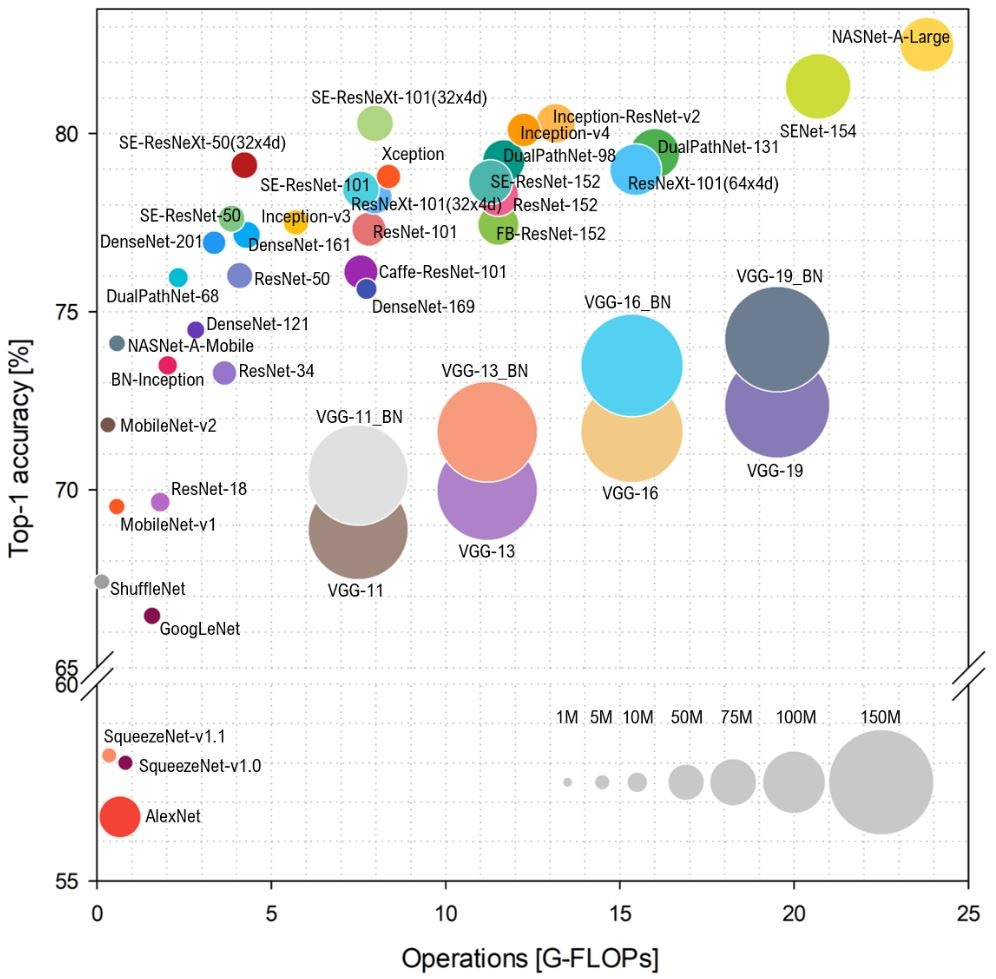
\includegraphics[width=0.7\linewidth,keepaspectratio]{./2_methodes/benchmark_deepLearning_Bianco2018}
		\caption[Graphique représentant la performance (« top-1 accuracy ») des grandes architectures sur le jeu de données ImageNet]{Graphique représentant la performance (« top-1 accuracy ») des grandes architectures sur le jeu de données ImageNet en fonction de la complexité de sa mise en œuvre  G-FLOPS = Giga FLoating-point Operations: nombre d’opérations numériques pour réaliser une inférence; la taille des disques correspond aux millions de paramètres à apprendre \citep{bianco_benchmark_2018}.}
	\label{figure_methodo3}
\end{center}
\end{figure}

\subsection{Stratégies d'entraînement des réseaux}

Tous les cas d’application et les jeux de données associés ont leurs propres spécificités, et s’il n’est pas possible de donner de recette magique, certaines bonnes pratiques permettent de maximiser les performances des réseaux entraînés \citep{he_bag_2019}. Par ailleurs, l’entraînement des réseaux est généralement coûteux en temps de calcul, et il existe une infinité de paramétrisations possibles, c’est pourquoi il convient d’adopter ces bonnes pratiques afin de converger au plus vite vers la paramétrisation optimale permettant de maximiser les performances du réseau.

\subsubsection{Déroulement de l'apprentissage}

L’apprentissage d’un RNC est un processus itératif au cours duquel les nombreux paramètres du modèle (l’architecture est déterminée au préalable), initialisés au hasard, sont ajustés par des méthodes numériques afin d’obtenir les meilleures performances prédictives. A chaque itération, un lot d’images (« batch ») choisies aléatoirement dans la base de données d’entraînement est fourni au réseau. Celui-ci va prédire une classe ou un score pour chaque image, et une fonction de coût (« loss function ») permettant de quantifier l’erreur du réseau dans sa prédiction pour le lot considéré. L’erreur est rétropropagée à travers tout le réseau afin de réajuster les poids des neurones, de sorte à améliorer la prédiction du réseau (i.e. diminuer la valeur de la fonction de coût), avec ce que l’on appelle une Descente de Gradient Stochastique (DGS ; « Stochastic Gradient Descent »). Lot par lot, tout le jeu de données d’entraînement est ainsi fourni au réseau et à chaque lot, les poids sont réajustés. Ceci correspond à ce que l’on appelle une « époque » (« epoch »), il en faut un certain nombre avant que le réseau n’atteigne ses meilleures performances et termine son apprentissage (\autoref{figure_methodo4}). A chaque époque, les cartes sont redistribuées, et les lots à nouveau formés aléatoirement depuis la base de données d’entraînement. Ainsi, chaque image sera vue par le réseau autant de fois que d’époques. L’apprentissage est considéré comme terminé lorsque, après un certain nombre d’époques, les performances du réseau cessent de croître.

\subsubsection{Le phénomène de surapprentissage (« over-fitting »)}

En machine learning, on parle de surapprentissage (« over-fitting ») lorsqu’un modèle prédictif obtient de meilleures performances sur le jeu de données d’entraînement (« training set ») que sur un jeu de données de validation (« validation set ») que le modèle n’a pas encore « vu » (voir haut de la \autoref{figure_methodo4}). Le modèle peut ainsi s’adapter si bien aux données d’entraînement qu’il en perd sa capacité de « généralisation », i.e. à s’appliquer avec des performances similaires sur un autre jeu de données de même nature. Du point de vue du compromis biais / variance, le phénomène de surapprentissage correspond à un modèle capable de s’adapter à tout jeu de données d’entraînement (faible biais), mais dont les paramètres devraient être fortement modifiés pour s’adapter à un autre jeu de données (forte variance). Cela est d’autant plus probable que le modèle est complexe, avec de nombreux paramètres, c’est pourquoi les RNC sont particulièrement sujets au surapprentissage \citep{li_gradient_2019}. On entend par « régularisation » l’ensemble des techniques permettant d’améliorer les capacités de généralisation d’un algorithme, i.e. diminuer son erreur sur le jeu de validation. Cette amélioration peut être réalisée au détriment de l’erreur d’entraînement.

Pour détecter le surapprentissage et mesurer la capacité d’un RNC à généraliser, il convient de séparer le jeu de données en trois lots : un jeu d’apprentissage (« training set »), un jeu de données de validation (« validation set ») et un jeu de données test (« test set ») :

\begin{itemize}
    \item \textbf{Jeu d’entraînement :} il correspond aux images données en entrée du réseau et qui permettent de réajuster les poids des neurones à chaque itération lors de l’apprentissage~;
    
    \item \textbf{Jeu de validation :} à chaque fois que les poids sont réajustés, le réseau mesure les performances sur ce jeu de données. Ce sont ces performances que l’on suit lors de l’apprentissage et qui permettent d’arrêter l’apprentissage avant de surapprendre le jeu d’entraînement~;
    
    \item \textbf{Jeu de test :} une fois l’apprentissage terminé, on mesure les performances du réseau sur ce jeu de données, entièrement nouveau pour lui et qui permet de mesurer les performances réelles du réseau et sa capacité à généraliser.
\end{itemize}

%%%%%%%%%%%%%%%%%%%%%%%%%%%%%%%%%%%%%%%%%%
%%% Figure methodo4: Entraînement CNNs %%%
%%%%%%%%%%%%%%%%%%%%%%%%%%%%%%%%%%%%%%%%%%
\begin{sidewaysfigure}
%\enlargethispage{.5cm}
\begin{figure}[H]
	\begin{center}
	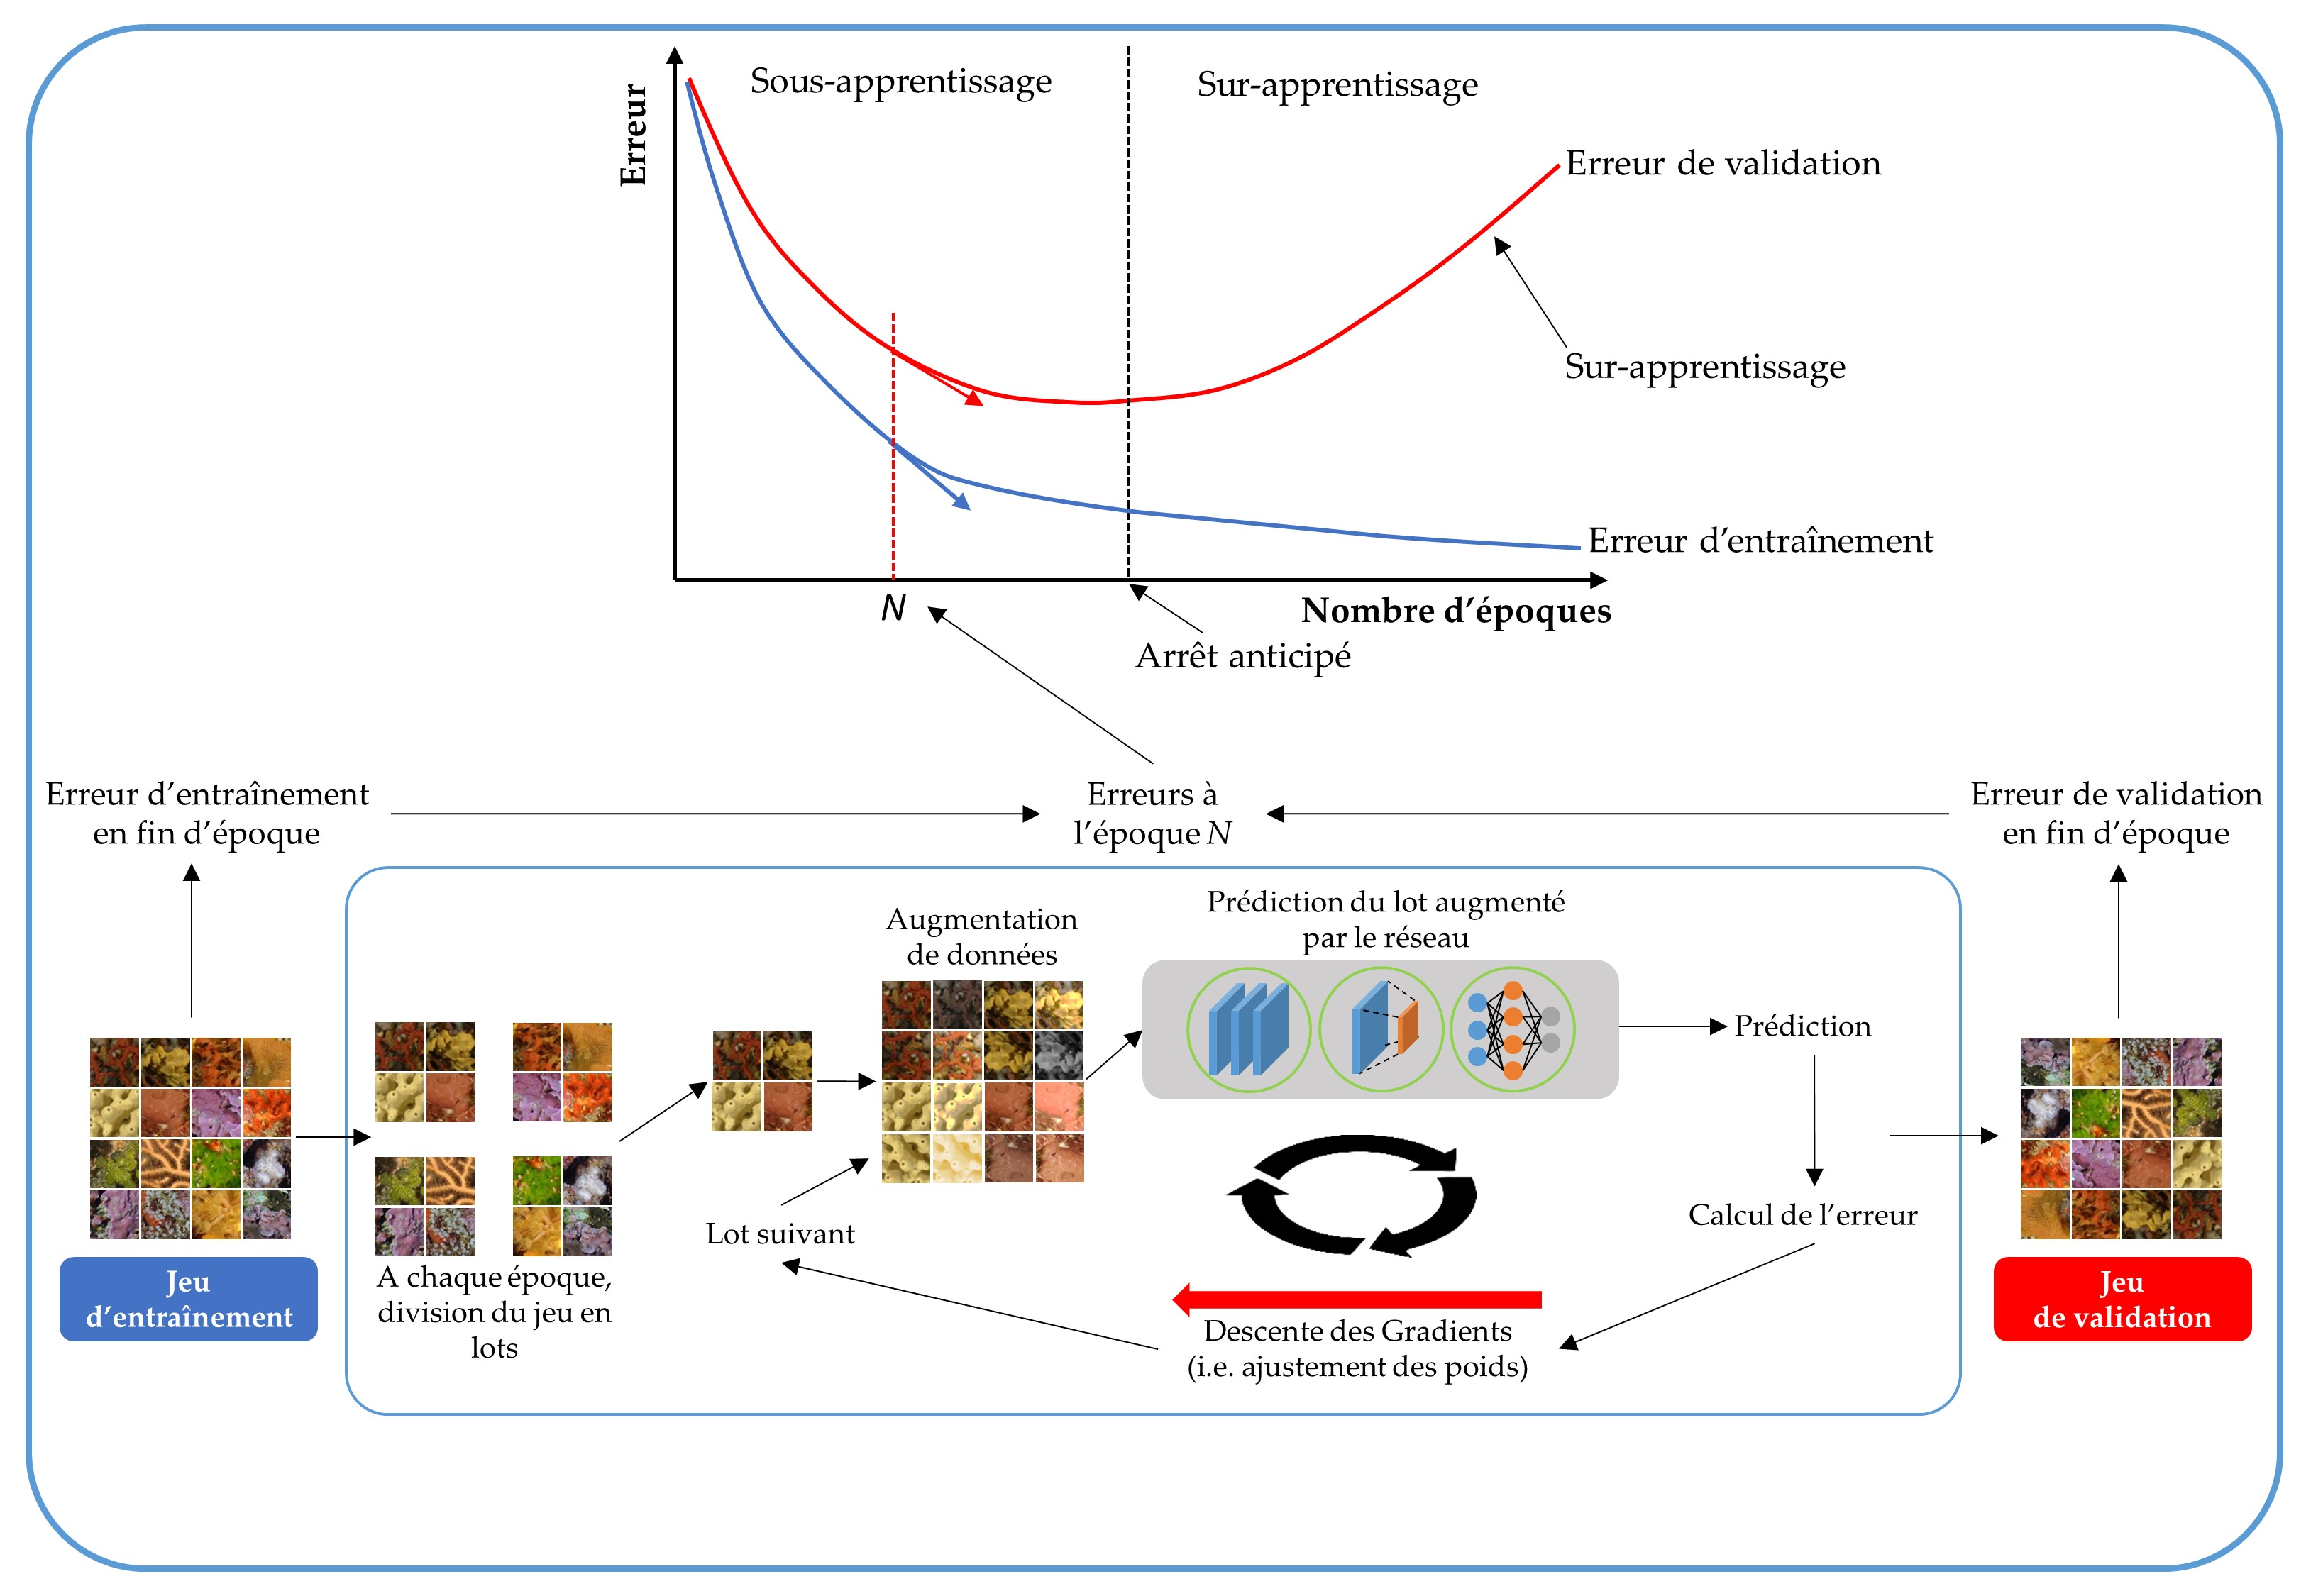
\includegraphics[width=\linewidth,keepaspectratio]{./2_methodes/encart_entrainement}
		\caption[Vision schématique de l’entraînement d’un réseau de neurones convolutifs à reconnaître une image]{Vision schématique de l’entraînement d’un réseau de neurones convolutifs à reconnaître une image.}
	\label{figure_methodo4}
\end{center}
\end{figure}
\end{sidewaysfigure}

La séparation en trois jeux de données dépend de la quantité de données, du nombre de classes et de la difficulté de la tâche à apprendre, mais il est préférable d’utiliser au moins la moitié du jeu de données pour l’entraînement, à condition que les données restantes soient suffisantes pour constituer des jeux de validation et de test représentatifs des variabilités inter et intra-classes.

\subsubsection{Choix de l’architecture et transfert de poids}

Comme vu précédemment, il existe de nombreuses architectures, plus ou moins performantes sur le jeu de données ImageNet, qui correspondent à différentes avancées techniques au fil des années (\autoref{figure_methodo3}). Cependant, le choix de l’architecture ne se dirigera pas nécessairement vers l’architecture ayant les meilleures performances sur le jeu de données ImageNet. En effet, les performances de classification dépendent globalement du nombre de paramètres du modèle, or plus ce nombre augmente plus la quantité de données requises et le temps d’entraînement augmentent. Par ailleurs, plus le rapport nombre de paramètres / quantité de données est élevé, plus le surapprentissage devient problématique. Le choix de l’architecture dépend donc de la quantité de données et de la complexité de la tâche de classification à réaliser. Pour autant, certaines architectures sont aujourd’hui dépassées et ne sont généralement plus utilisées ; c’est le cas d’AlexNet qui a les moins bonnes performances (relativement aux autres architectures de RNC), pour un nombre de paramètres assez important, ou encore VGGNet qui a des performances aujourd’hui considérées comme moyennes pour un nombre très élevé de paramètres.

Dans le cas d’un entraînement à partir de zéro (« from scratch »), l’ensemble des paramètres (i.e. poids) du modèle sont fixés aléatoirement, et leur valeur est ajustée par la DGS à chaque itération jusqu’à convergence. Cependant, il est possible pour les architectures connues d’initialiser les poids avec les valeurs ayant permis de maximiser les performances sur la base de données ImageNet (i.e. transfert de poids ou « transfer learning ») et réaliser l’entraînement pour la tâche souhaitée en ajustant tout ou partie des poids à partir de ces valeurs (i.e. ajustement ou « fine-tuning »). En effet, les premières couches sont relativement peu spécifiques et facilement transférables d’une tâche à l’autre \citep{yosinski_how_2014}. Cette technique a fait ses preuves \citep{huh_what_2016} et elle est couramment utilisée, notamment dans le cas de jeux de données de petite taille \citep{ng_deep_2015}. Il a été montré que les résultats sont d’autant meilleurs que la tâche de classification est proche de la tâche d’origine, mais qu’ils peuvent surpasser les performances atteintes par initialisation aléatoire y compris dans le cas de tâches plus éloignées \citep{yosinski_how_2014}. Par ailleurs, le transfert de poids pourrait augmenter les capacités de généralisation d’un réseau, y compris après l’ajustement des poids \citep{yosinski_how_2014}.

Enfin, comme en apprentissage classique, l’utilisation d’ensembles de réseaux permet parfois d’augmenter les performances prédictives tout en conservant la capacité de généralisation \citep{mehdipour_ghazi_open-set_2016, perez_solo_2019}. Les réseaux composant l’ensemble sont généralement entraînés séparément, puis la décision finale est déterminée par combinaison des prédictions : souvent en prenant la moyenne des prédictions, ou bien en entraînant un perceptron multicouche sur les descripteurs extraits par chacun des réseaux \citep{rokach_ensemble-based_2010}.

\subsubsection{Augmentation de données}

La méthode la plus simple et commune pour régulariser l’apprentissage est ce qu’on appelle « l’augmentation de données » (« data augmentation ») : des images sont générées à la volée à partir des exemples de la base de données d’entraînement, en appliquant des transformations simples telles que des translations, zooms, rotations et miroir / reflet \citep{aggarwal_neural_2018}. En effet, dans la majorité des cas, ces transformations n’affectent en rien les propriétés de l’image et son contenu, ce qui permet d’augmenter virtuellement la taille du jeu de données et d’améliorer les capacités du réseau à reconnaître un objet dans différentes conditions (i.e. améliore la généralisation) \citep{wong_understanding_2016}. Par exemple, une banane reste une banane quelle que soit son orientation. Augmenter les données en prenant différents niveaux de rotation de l’image et en prenant le miroir et le reflet de chaque image améliorera les capacités du réseau à reconnaître une banane dans toutes les orientations. Il convient en revanche de s’assurer que les transformations infligées aux images correspondent à des situations observables et ne modifient pas les propriétés de son contenu. Par exemple, il serait mal venu d’appliquer des rotations ou un effet miroir aux chiffres manuscrits de la base de données MNIST \citep{lecun_gradient-based_1998}, car les chiffres sont des objets orientés (et un « 6 » à l’envers correspond à un « 9 »).

\subsubsection{Autres méthodes de régularisation}

Il existe un grand nombre de méthodes permettant de minimiser l’erreur d’entraînement tout en maximisant la capacité du réseau à généraliser. Les principales techniques utilisées sont les suivantes :

\paragraph{Taille des lots (« batch size »)}

La taille des lots (ou « batch size ») correspond au nombre d’images analysées par le réseau en cours d’apprentissage à chaque itération. Si le jeu d’entraînement contient N images et l’on choisit une taille de lot B, le nombre d’itérations par époque sera de N / B. A chaque itération, B images sont envoyées au réseau qui réalise ses prédictions, mesure les performances et rétropropage l’erreur via la DGS. S’il a été montré que de petites tailles de lots permettent une meilleure généralisation et convergence lors de l’entraînement \citep{wilson_general_2003, keskar_large-batch_2017}, l’utilisation de lots de grande taille permet d’accélérer considérablement les calculs en augmentant l’efficacité d’utilisation des processeurs par la parallélisation des calculs \citep{das_distributed_2016}. Le choix de la taille des lots relève donc d’un compromis qui va dépendre de la nature de la tâche de classification, de la variabilité des données et des caractéristiques de la machine d’entraînement. Par ailleurs, il est également possible de rendre cette taille dynamique au cours des époques conjointement au taux d’apprentissage, pour permettre d’accélérer les calculs tout en maximisant la généralisation et la bonne convergence de l’apprentissage \citep{balles_coupling_2017}.

\paragraph{Taux d’apprentissage (« learning rate »)}

Comme pour tout problème d’optimisation, l’entraînement d’un RNC est un processus itératif où des paramètres sont ajustés à chaque itération afin de minimiser une fonction de coût. En apprentissage profond, le taux d’apprentissage (« learning rate ») contrôle l’intensité de l’ajustement des poids de neurones à chaque itération (chaque évaluation d’un lot) afin de minimiser la fonction de coût via la DGS ; en d’autres termes, ce paramètre contrôle la vitesse à laquelle le réseau doit apprendre de ses erreurs. Ce paramètre est important, car s’il est trop faible, la convergence risque d’être très longue voir ne jamais atteindre la solution optimale, et s’il est trop fort, l’algorithme pourra se rapprocher rapidement d’une solution optimale puis osciller autour de cette position voire atteindre un état instable et diverger \citep{aggarwal_neural_2018}. C’est pourquoi le taux d’apprentissage est généralement géré dynamiquement par des algorithmes plus ou moins complexes comme l’algorithme Adam \citep{kingma_adam:_2014}, largement utilisé en apprentissage profond.

\paragraph{Décrochage de neurones (« dropout ») }

Le décrochage (« dropout ») est une méthode de régularisation qui utilise l’inactivation de certains neurones des couches denses pendant la phase d’entraînement, aléatoirement sélectionnés à chaque itération \citep{srivastava_dropout_2014}. Cette méthode permet également d’éviter la coadaptation des détecteurs de caractéristiques de l’image \citep{hinton_improving_2012}. C’est un puissant outil de régularisation qui peut être perçu comme une moyenne de modèles. En pratique, il est commun d’inactiver aléatoirement entre 20 et 50 \% des neurones parmi les couches denses à chaque itération \citep{aggarwal_neural_2018}.

\paragraph{Normalisation des lots (« batch normalisation »)}

Une des difficultés rencontrées lors de l’entraînement des RNC est la distribution des entrées de chaque couche qui change au cours de l’entraînement, au fur et à mesure que les paramètres des couches précédentes sont modifiés par la DGS. La normalisation des lots (« batch normalisation ») élimine ce problème, connu sous le nom de « internal covariate shift », en normalisant tous les lots lors de l’entraînement \citep{ioffe_batch_2015}. Cette normalisation permet d’utiliser des taux d’apprentissages plus importants et donc d’accélérer la convergence, mais également de régulariser l’apprentissage \citep{luo_towards_2019} avec un comportement similaire au décrochage de neurones \citep{szegedy_going_2015}.

\paragraph{Arrêt anticipé (« early stopping »)}

Lors des premières époques, les performances du réseau ont tendance à augmenter tant en entraînement qu’en validation, jusqu’à un moment où les performances en validation commencent à retomber tandis que celles en entraînement continuent de s’améliorer (\autoref{figure_methodo4}). En effet, il a été démontré que durant les premières époques, le réseau tend à apprendre à reconnaître les principales caractéristiques de chaque classe, et si l’on poursuit un grand nombre d’époques, il finit par apprendre les spécificités du jeu d’entraînement et perd toute capacité à généraliser \citep{li_gradient_2019}. Le corollaire est que l’entraînement d’un RNC est relativement robuste à la présence de bruit ou d’erreurs dans la donnée ; pourvu que l’entraînement soit arrêté avant le surapprentissage, le réseau apprendra les caractéristiques générales des classes en s’affranchissant du bruit. Mais du fait de leur très grand nombre de paramètres, les RNC ont la capacité de surapprendre n’importe quel jeu de données, y compris un jeu de données composé uniquement de bruit \citep{zhang_understanding_2017}. Par ailleurs, même en maîtrisant le surapprentissage par les méthodes précédentes, le coût d’entraînement des grosses architectures peut être important et il n’est pas toujours souhaitable de tripler le temps de calcul pour une augmentation non significative des performances. Il apparaît donc indispensable d’arrêter l’entraînement au moment opportun, i.e. après avoir appris les caractéristiques permettant de distinguer les classes les unes des autres, sans surapprendre les spécificités de chaque exemple du jeu d’entraînement.

L’arrêt anticipé de l’entraînement, ou « early stopping », est provoqué par la satisfaction d’un ou plusieurs critères objectifs qui permettent de détecter le moment opportun pour arrêter l’apprentissage et obtenir les meilleures capacités de généralisation. La règle théorique est simple : arrêter l’entraînement dès que l’erreur de validation est supérieure à celle calculée à la dernière époque. Cependant, la réalité est souvent plus chaotique avec des courbes dont les fluctuations ne permettent souvent pas un raisonnement aussi simple \citep{prechelt_early_1998}. Par ailleurs, le surapprentissage ne démarre généralement qu’après un ralentissement de la décroissance de l’erreur d’entraînement, donc une augmentation soudaine de l’erreur de validation a toutes les chances d’être « réparée » si l’erreur d’entraînement est encore en phase de décroissance importante. C’est pourquoi le critère d’arrêt choisi est généralement le ratio de la pente d’erreur d’entraînement sur celle de validation ou bien l’arrêt après $N$ époques consécutives avec une augmentation de l’erreur de validation (auquel cas on retient la solution correspondant à la dernière époque avant cette série).

\medskip

\setlength{\fboxsep}{5pt}
\setlength{\fboxrule}{0.6pt}
\noindent\framebox{%
  \begin{minipage}{\linewidth}
    Les RNC ont gagné en \textbf{précision} et en \textbf{efficacité} grâce au développement d’architectures de plus en plus performantes, mais leurs \textbf{très grands nombres de paramètres} les rendent sensibles au \textbf{surapprentissage}. Heureusement, différentes stratégies de \textbf{régularisation} ont été développées au cours du temps et permettent de contrôler ce surapprentissage afin d’entraîner des RNC à réaliser des \textbf{tâches complexes} sur des jeux de données de \textbf{natures très différentes}.
  \end{minipage}
}

\subsection{Applications en écologie marine}

Par leur incroyable performance et leur capacité d’adaptation à des jeux de données et des tâches de natures très variées, les RNC ont rapidement trouvé de très nombreuses applications, tant en recherche que dans l’industrie. L’écologie ne fait pas exception à la règle, et le nombre d’articles scientifiques utilisant des RNC a littéralement explosé depuis 2015 \citep{christin_applications_2019} (\autoref{figure_methodo5}). Les cas d’application sont très divers, depuis la reconnaissance d’espèces ou d’individus à l’estimation de ressources en passant par l’évaluation de la biodiversité d’un habitat.

%%%%%%%%%%%%%%%%%%%%%%%%%%%%%%%%%%%%%%%%%%%%%%%%%
%%% Figure methodo5: Utilisation CNN écologie %%%
%%%%%%%%%%%%%%%%%%%%%%%%%%%%%%%%%%%%%%%%%%%%%%%%%
\begin{figure}[H]
	\begin{center}
	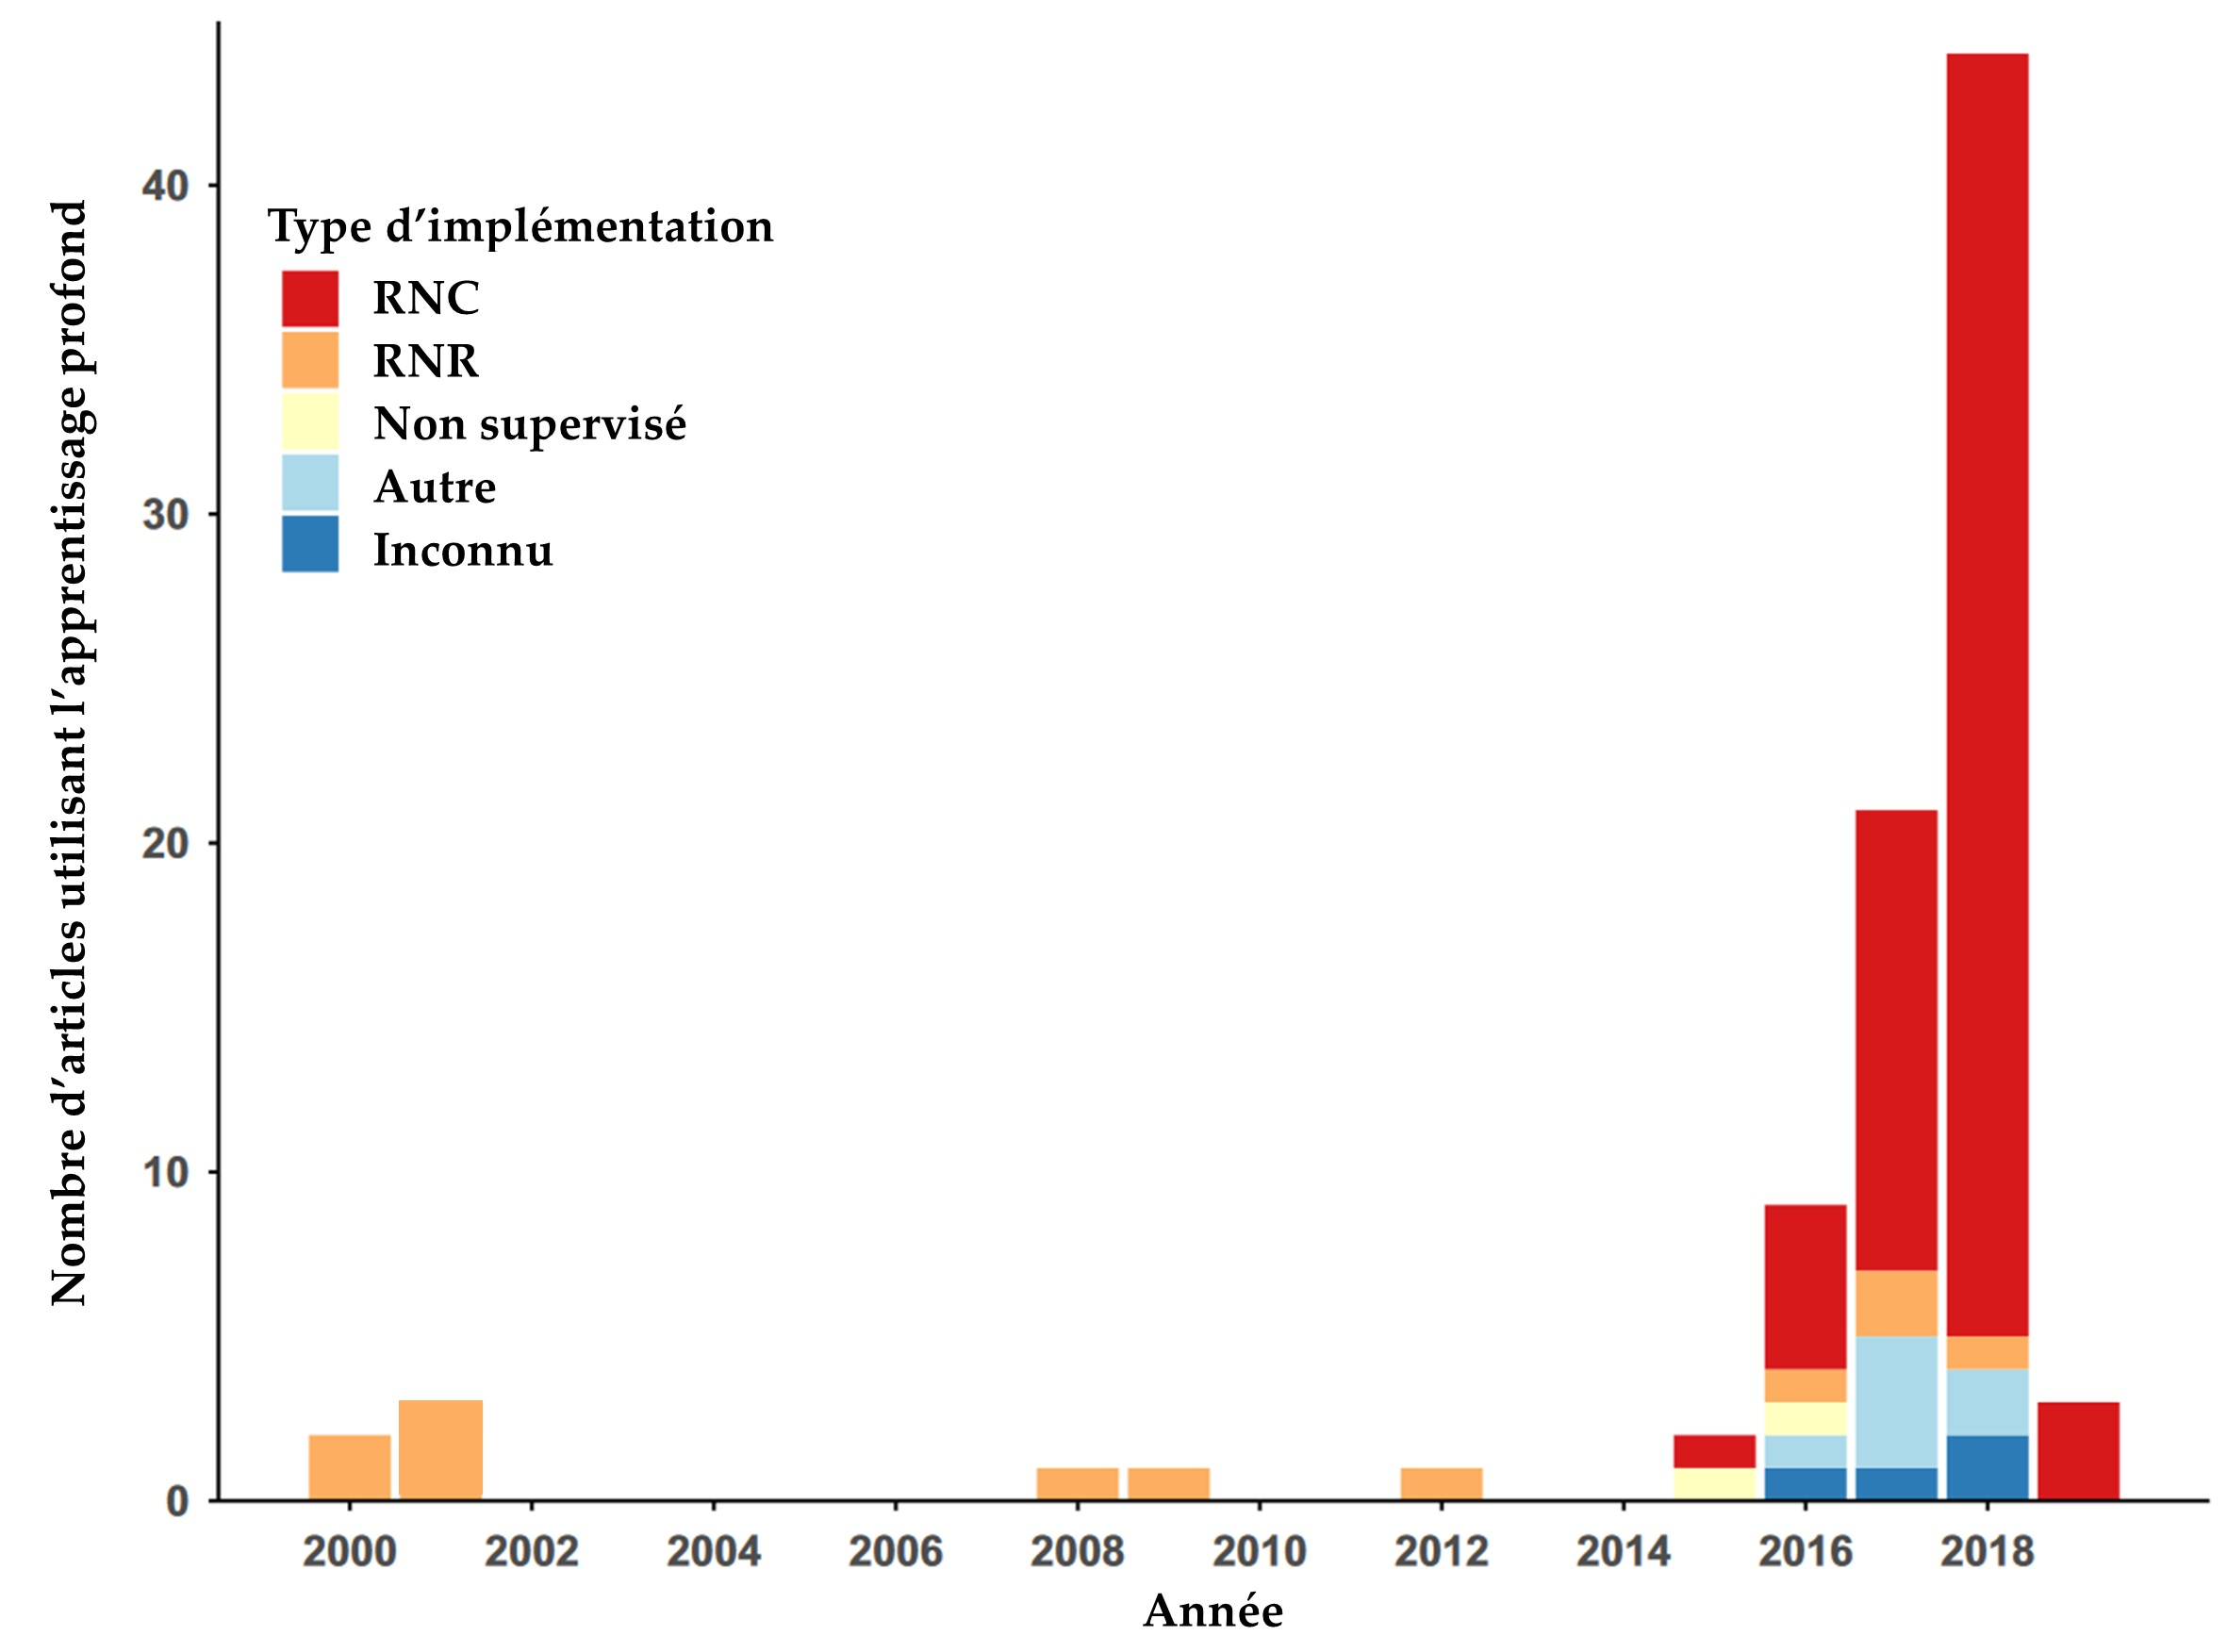
\includegraphics[width=0.7\linewidth,keepaspectratio]{./2_methodes/CNN_ecology}
		\caption[Utilisation d’algorithmes à apprentissage profond en écologie]{Utilisation d’algorithmes à apprentissage profond en écologie (adapté de \citet{christin_applications_2019}). RNC = Réseau de Neurones Convolutifs, RNR = Réseau de Neurones Récurrent.}
	\label{figure_methodo5}
\end{center}
\end{figure}

Si les RNC ont prouvé leurs redoutables performances sur des jeux de données bien particuliers avec des classes distinctes, les applications à des cas plus complexes comme la reconnaissance d’espèces soulèvent de nouveaux problèmes. Dans le cas d’images sous-marines en particulier, la variabilité des conditions lumineuses ainsi que la diversité morphologique intraspécifique des espèces benthiques rendent la tâche de classification particulièrement complexe \citep{beijbom_automated_2012}. Pour autant, les RNC ont déjà prouvé à plusieurs reprises qu’ils étaient appropriés pour la reconnaissance d’images benthiques \citep{raphael_neural_2020}. En particulier, la reconnaissance d’images de coraux par des RNC a atteint de très bonnes performances, notamment la discrimination entre corail / non corail \citep{manderson_robotic_2017, williams_leveraging_2019}. Ils ont également atteint 90 \% de bonnes classifications pour un problème à 10 classes de corail et substrat \citep{king_comparison_2018}, et il existe aujourd’hui un réseau entraîné sur un grand jeu de données d’images annotées de récifs coralliens, capable de reconnaître les principales espèces de corail : CoralNet \citep{beijbom_towards_2015}. Ce projet collaboratif s’est largement développé depuis sa création et compte aujourd’hui près de 50 000 000 d’annotations expertes sur 1 362 000 images issues de 1 451 sources à travers le monde (\autoref{figure_methodo6}).

%%%%%%%%%%%%%%%%%%%%%%%%%%%%%%%%%%%%%%%%%%%%%%
%%% Figure methodo6: Cartographie coralNet %%%
%%%%%%%%%%%%%%%%%%%%%%%%%%%%%%%%%%%%%%%%%%%%%%
\begin{figure}[H]
	\begin{center}
	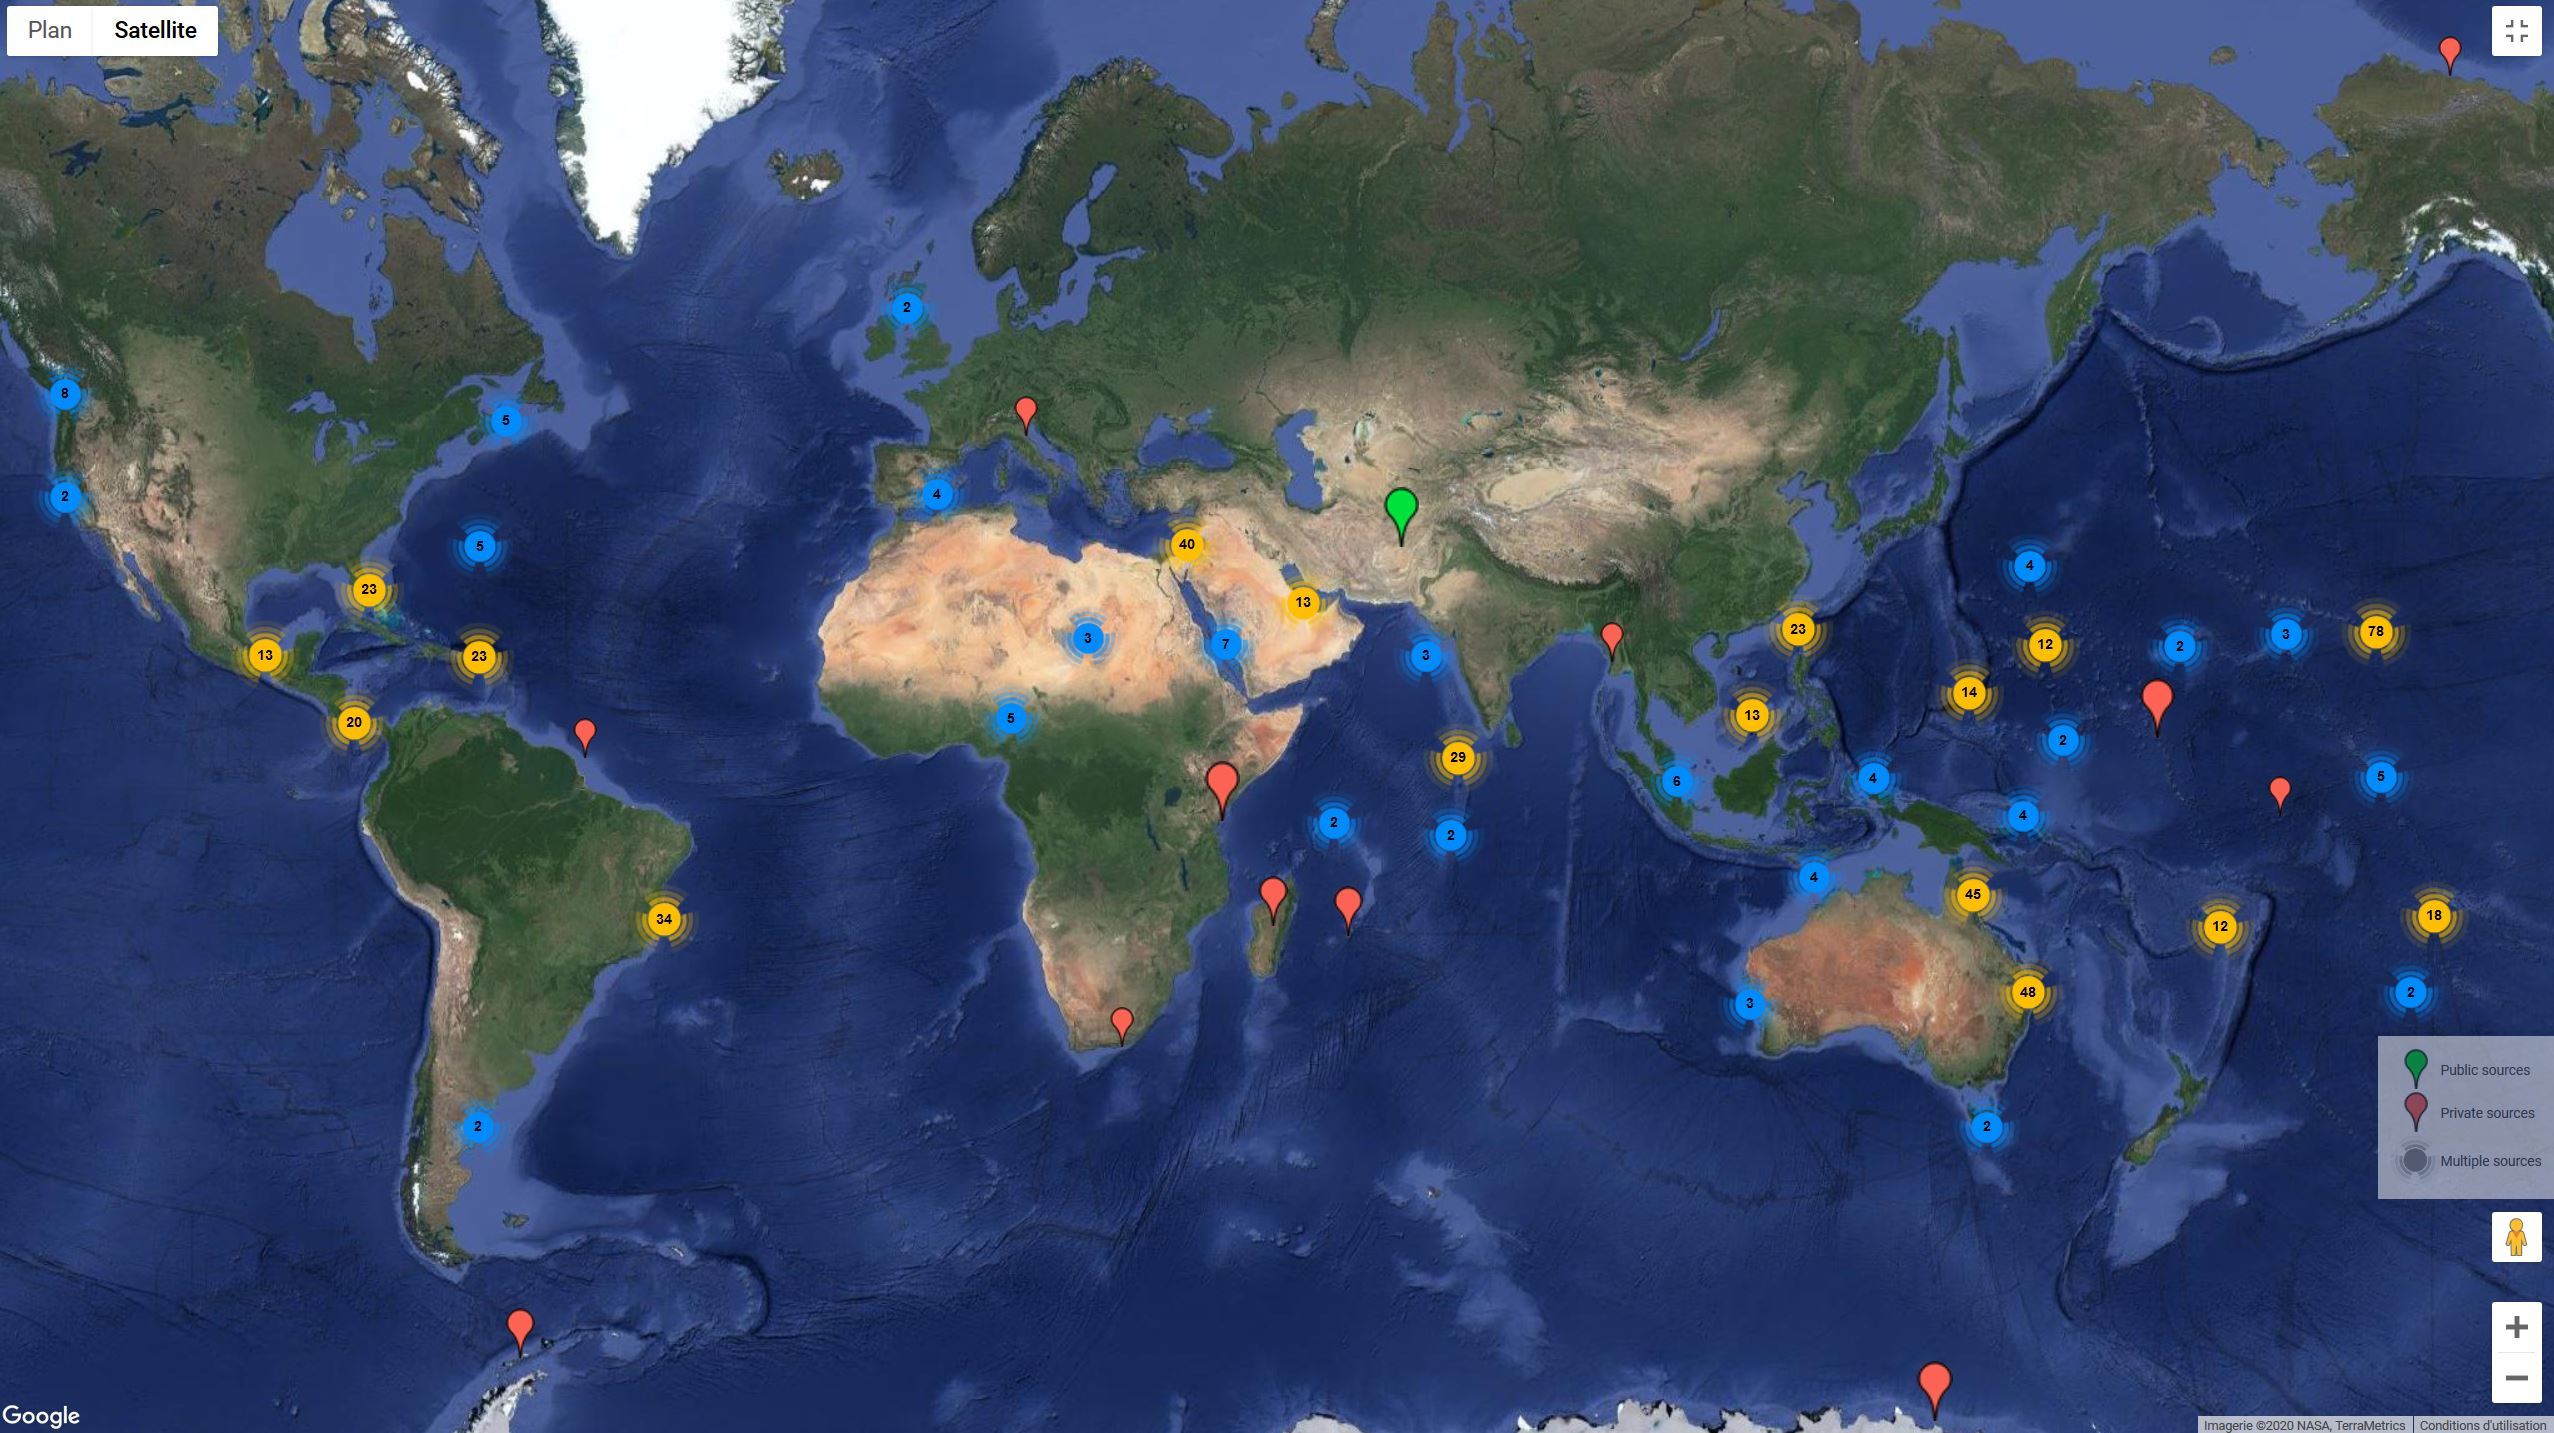
\includegraphics[width=\linewidth,keepaspectratio]{./2_methodes/coralnet_map}
		\caption[Localisation des sources d’images utilisées par CoralNet]{Localisation des sources d’images utilisées par CoralNet (source : coralnet.ucsd.edu).}
	\label{figure_methodo6}
\end{center}
\end{figure}

\setlength{\fboxsep}{5pt}
\setlength{\fboxrule}{0.6pt}
\noindent\framebox{%
  \begin{minipage}{\linewidth}
    Les RNC sont de \textbf{puissants algorithmes} permettant d’\textbf{analyser} et \textbf{interpréter} le contenu d’images de \textbf{natures très différentes}. Depuis 2015, ils sont de plus en plus utilisés en écologie, notamment en \textbf{écologie marine} pour \textbf{l’identification d’images benthiques}, où ils ont prouvé leur capacité à identifier avec précision \textbf{plusieurs catégories de substrat} et de \textbf{corail}. Ces résultats ont motivé l’entraînement d’un RNC pour la reconnaissance d’espèces du \textbf{coralligène} dans le cadre du réseau RECOR, qui est un habitat de complexité similaire aux récifs coralliens, pour lesquels aucune application de RNC n’a été décrite à ce jour.
  \end{minipage}
}

\newpage

\section[La photogrammétrie sous-marine : principes et contraintes]{La photogrammétrie sous-marine : principes et contraintes}\label{methodes.2}

\subsection{Définition}

Il existe de nombreuses situations et applications pour lesquelles il est nécessaire de mesurer des coordonnées, des distances, des surfaces ou encore des volumes. Pour les cas les plus triviaux, un simple outil de mesure peut suffire, mais il existe de nombreux cas où cela ne permet pas de réaliser les mesures souhaitées : surface complexe, précision importante requise, impossibilité de venir au contact de l’objet d’étude, taille de l’objet, ou encore la nécessité de figer un objet amené à disparaître. L’utilisation de photographies en télédétection peut répondre à certains de ces besoins plus complexes, mais leur analyse se limite à la détermination de coordonnées 2D. Afin d’obtenir des coordonnées en 3D, il faut utiliser d’autres méthodes telles que le LiDAR (laser), l’échosondeur, ou encore la photogrammétrie.

La photogrammétrie, ou « science de la mesure sur photos » \citep{linder_digital_2016}, est une technique permettant aujourd’hui de reconstruire en 3D un objet ou une scène à partir d’un grand nombre de photos prises sous différents angles de vue. Son principe de fonctionnement se base sur la vision stéréoscopique dont nous sommes nous-mêmes dotés : si nous disposons de deux (ou plus) images d’un même objet prises en différents points de vue, il est possible de calculer les coordonnées 3D de tout point de l’objet qui est visible sur les deux images. Contrairement à d’autres techniques de télédétection comme le LiDAR ou le sonar, la photogrammétrie permet de renseigner également sur la couleur et de produire un modèle de surface 3D coloré réaliste. Par la même occasion, elle permet de documenter la scène avec les mêmes images utilisées pour la reconstruction, ce qui lui confère un avantage supplémentaire. En revanche, de même qu’une image n’est qu’une représentation de la réalité, simplifiée par discrétisation (pixels) et par quantification (nombre fini de pixels différents), la photogrammétrie permet de reconstruire un « modèle 3D » qui n’est jamais qu’une représentation simplifiée de la réalité et repose sur certaines hypothèses. Par ailleurs, la photogrammétrie présente plusieurs limites qui peuvent orienter certains besoins vers d’autres méthodes d’acquisition 3D : elle nécessite une source de lumière, elle est dépendante de la visibilité et sensible aux occlusions, elle ne permet pas de capturer des objets en mouvement à l’aide d’un seul capteur, sa précision peut être parfois inférieure à celle d’autres méthodes telles que le LiDAR…

La photogrammétrie a connu un important essor ces dernières années grâce à l’amélioration des algorithmes et à l’explosion de la puissance de calcul, notamment via l’utilisation des cartes graphiques (GPU). Par ailleurs, la force des algorithmes actuels capables d’auto-calibrer les paramètres optiques de l’appareil photo durant le processus de reconstruction \citep{forstner_photogrammetric_2016} permet d’utiliser à peu près n’importe quel appareil photo pour les reconstructions, bien que la qualité du capteur et de l’optique influencent la qualité de la reconstruction \citep{linder_digital_2016}. Elle est aujourd’hui utilisée pour de nombreuses applications, depuis l’architecture et l’urbanisme jusqu’à l’écologie, en passant par l’industrie, le cinéma, l’archéologie, la géologie, la reconstruction de scènes de crime… (\autoref{figure_methodo7}).

%%%%%%%%%%%%%%%%%%%%%%%%%%%%%%%%%%%%%%%%%%%%%%%%%%
%%% Figure methodo7: Applications générales PG %%%
%%%%%%%%%%%%%%%%%%%%%%%%%%%%%%%%%%%%%%%%%%%%%%%%%%
\begin{figure}[H]
	\begin{center}
	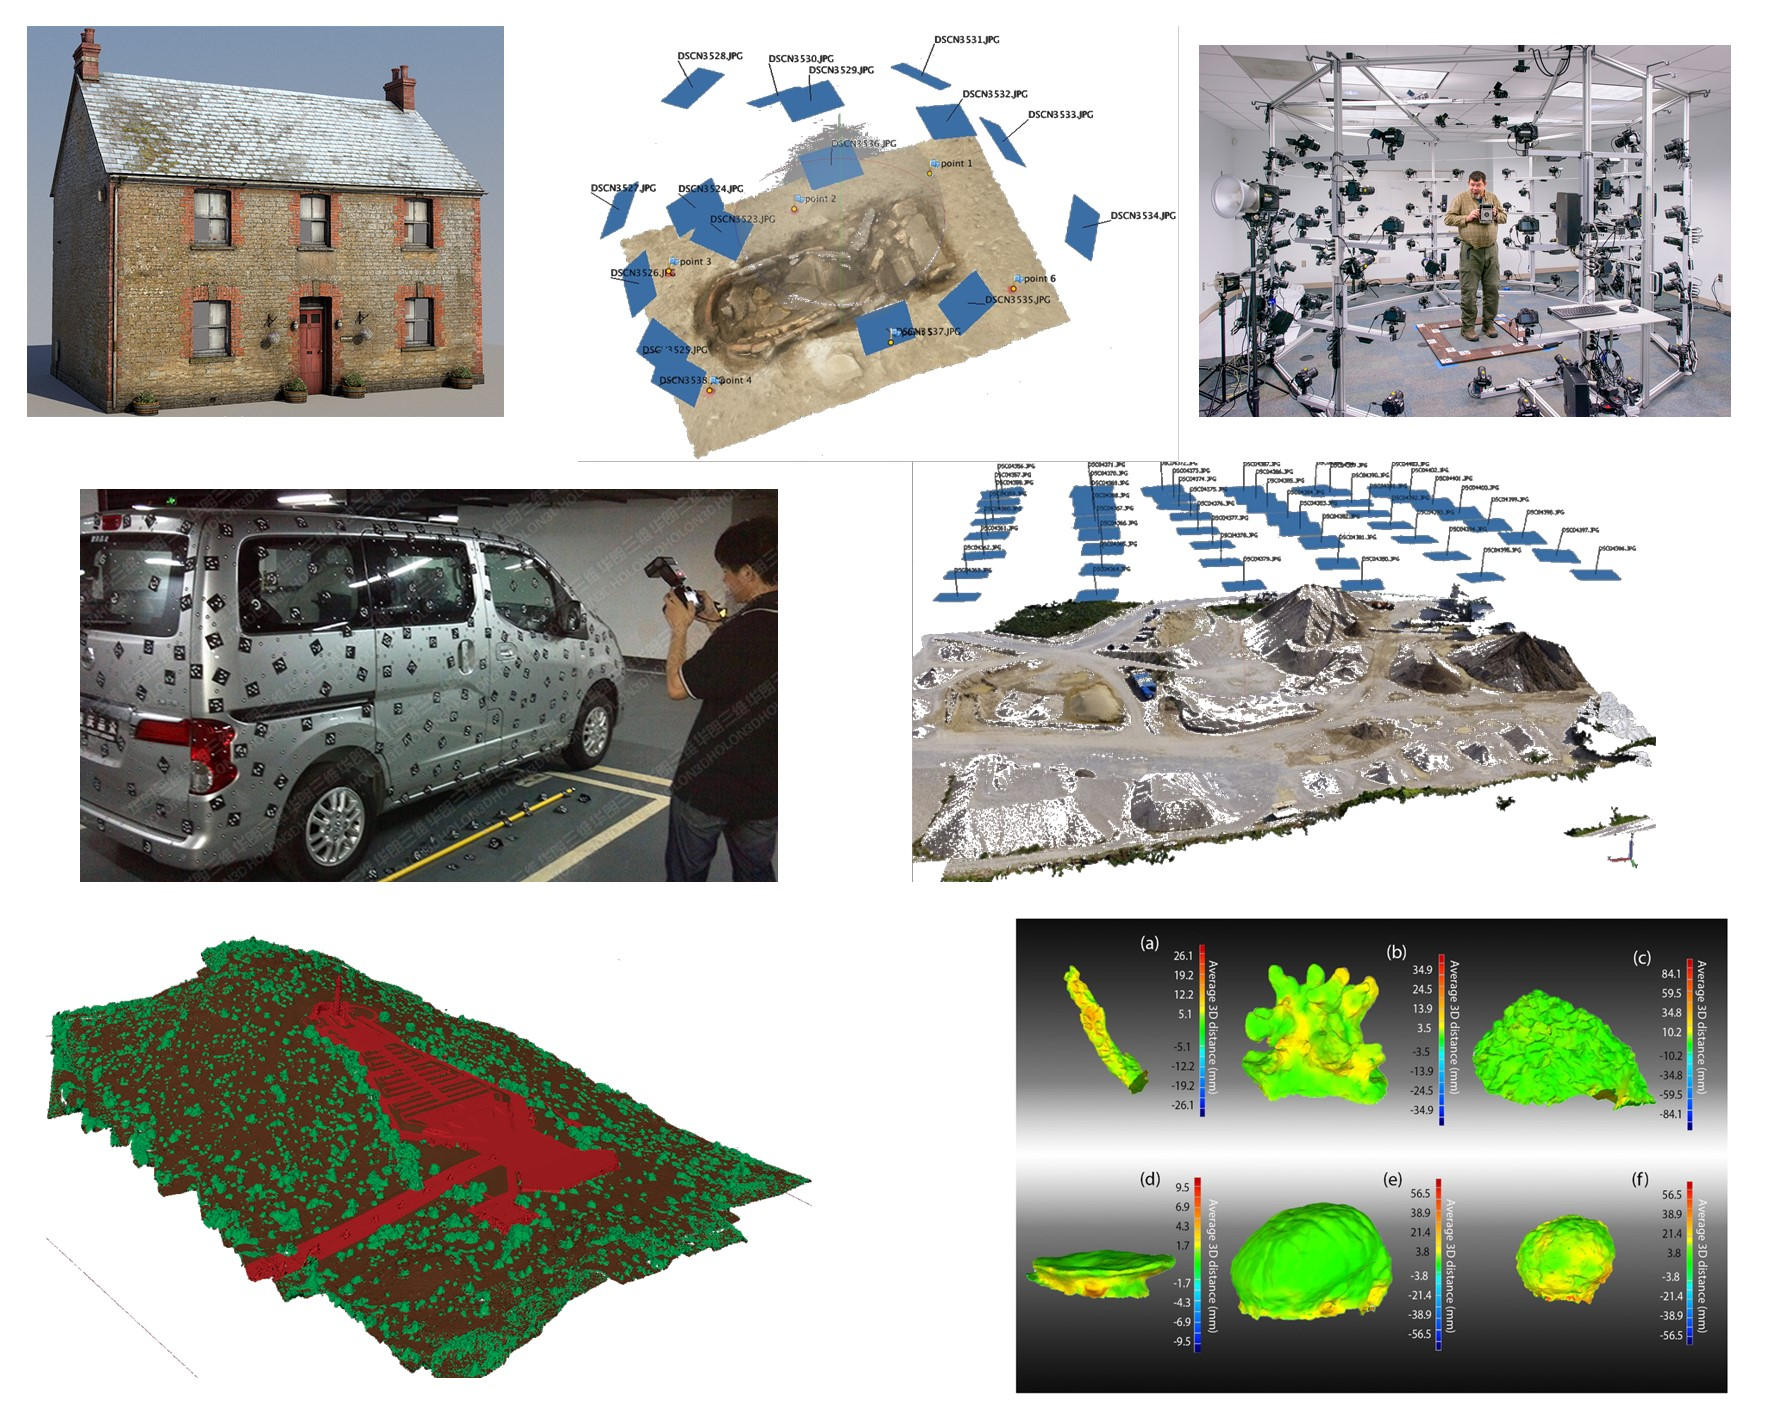
\includegraphics[width=\linewidth,keepaspectratio]{./2_methodes/applications_PG}
		\caption[Exemples d’applications de la photogrammétrie]{Exemples d’applications de la photogrammétrie. De haut en bas et de gauche à droite : architecture, archéologie, cinéma, industrie, exploitation de minerais, écologie forestière, écologie marine.}
	\label{figure_methodo7}
\end{center}
\end{figure}

\subsection{Théorie générale : les étapes de la reconstruction}

La photogrammétrie est une technique de traitement d’images qui a pour objectif la reconstruction 3D d’un objet observé sous différentes perspectives. Si à ses débuts, elle se limitait à l’interprétation manuelle de paires d’images obtenues par stéréophotogrammétrie pour reconstruire quelques coordonnées 3D et réaliser des mesures de longueur ou de hauteur, elle permet aujourd’hui d’automatiser l’ensemble du processus de reconstruction 3D de surfaces complexes. L’ensemble du processus photogrammétrique suit un enchaînement de traitements numériques pour passer des images 2D au modèle 3D (Figure 27) :

\begin{enumerate}
    \item Détection de points d’intérêt (« keypoints »)~;
    
    \item Reconnaissance des points homologues (« tie points »)~;
    
    \item Aéro-triangulation~;
    
    \item Densification du nuage de points~;
    
    \item Construction du maillage~;
    
    \item Application d’une texture.
\end{enumerate}

L’objectif de cette section n’est pas de rentrer dans le détail des calculs mathématiques associés à la reconstruction 3D, mais de fournir au lecteur une vision simplifiée permettant de comprendre le fonctionnement et l’enchaînement des différentes étapes, depuis l’analyse des images jusqu’à la production du modèle 3D réaliste.


%%%%%%%%%%%%%%%%%%%%%%%%%%%%%%%%%%%%%%%%%%%%%%%%%%%%%%%%%%%
%%% Figure methodo8: Les étapes de la reconstruction 3D %%%
%%%%%%%%%%%%%%%%%%%%%%%%%%%%%%%%%%%%%%%%%%%%%%%%%%%%%%%%%%%
\begin{sidewaysfigure}
\begin{figure}[H]
	\begin{center}
	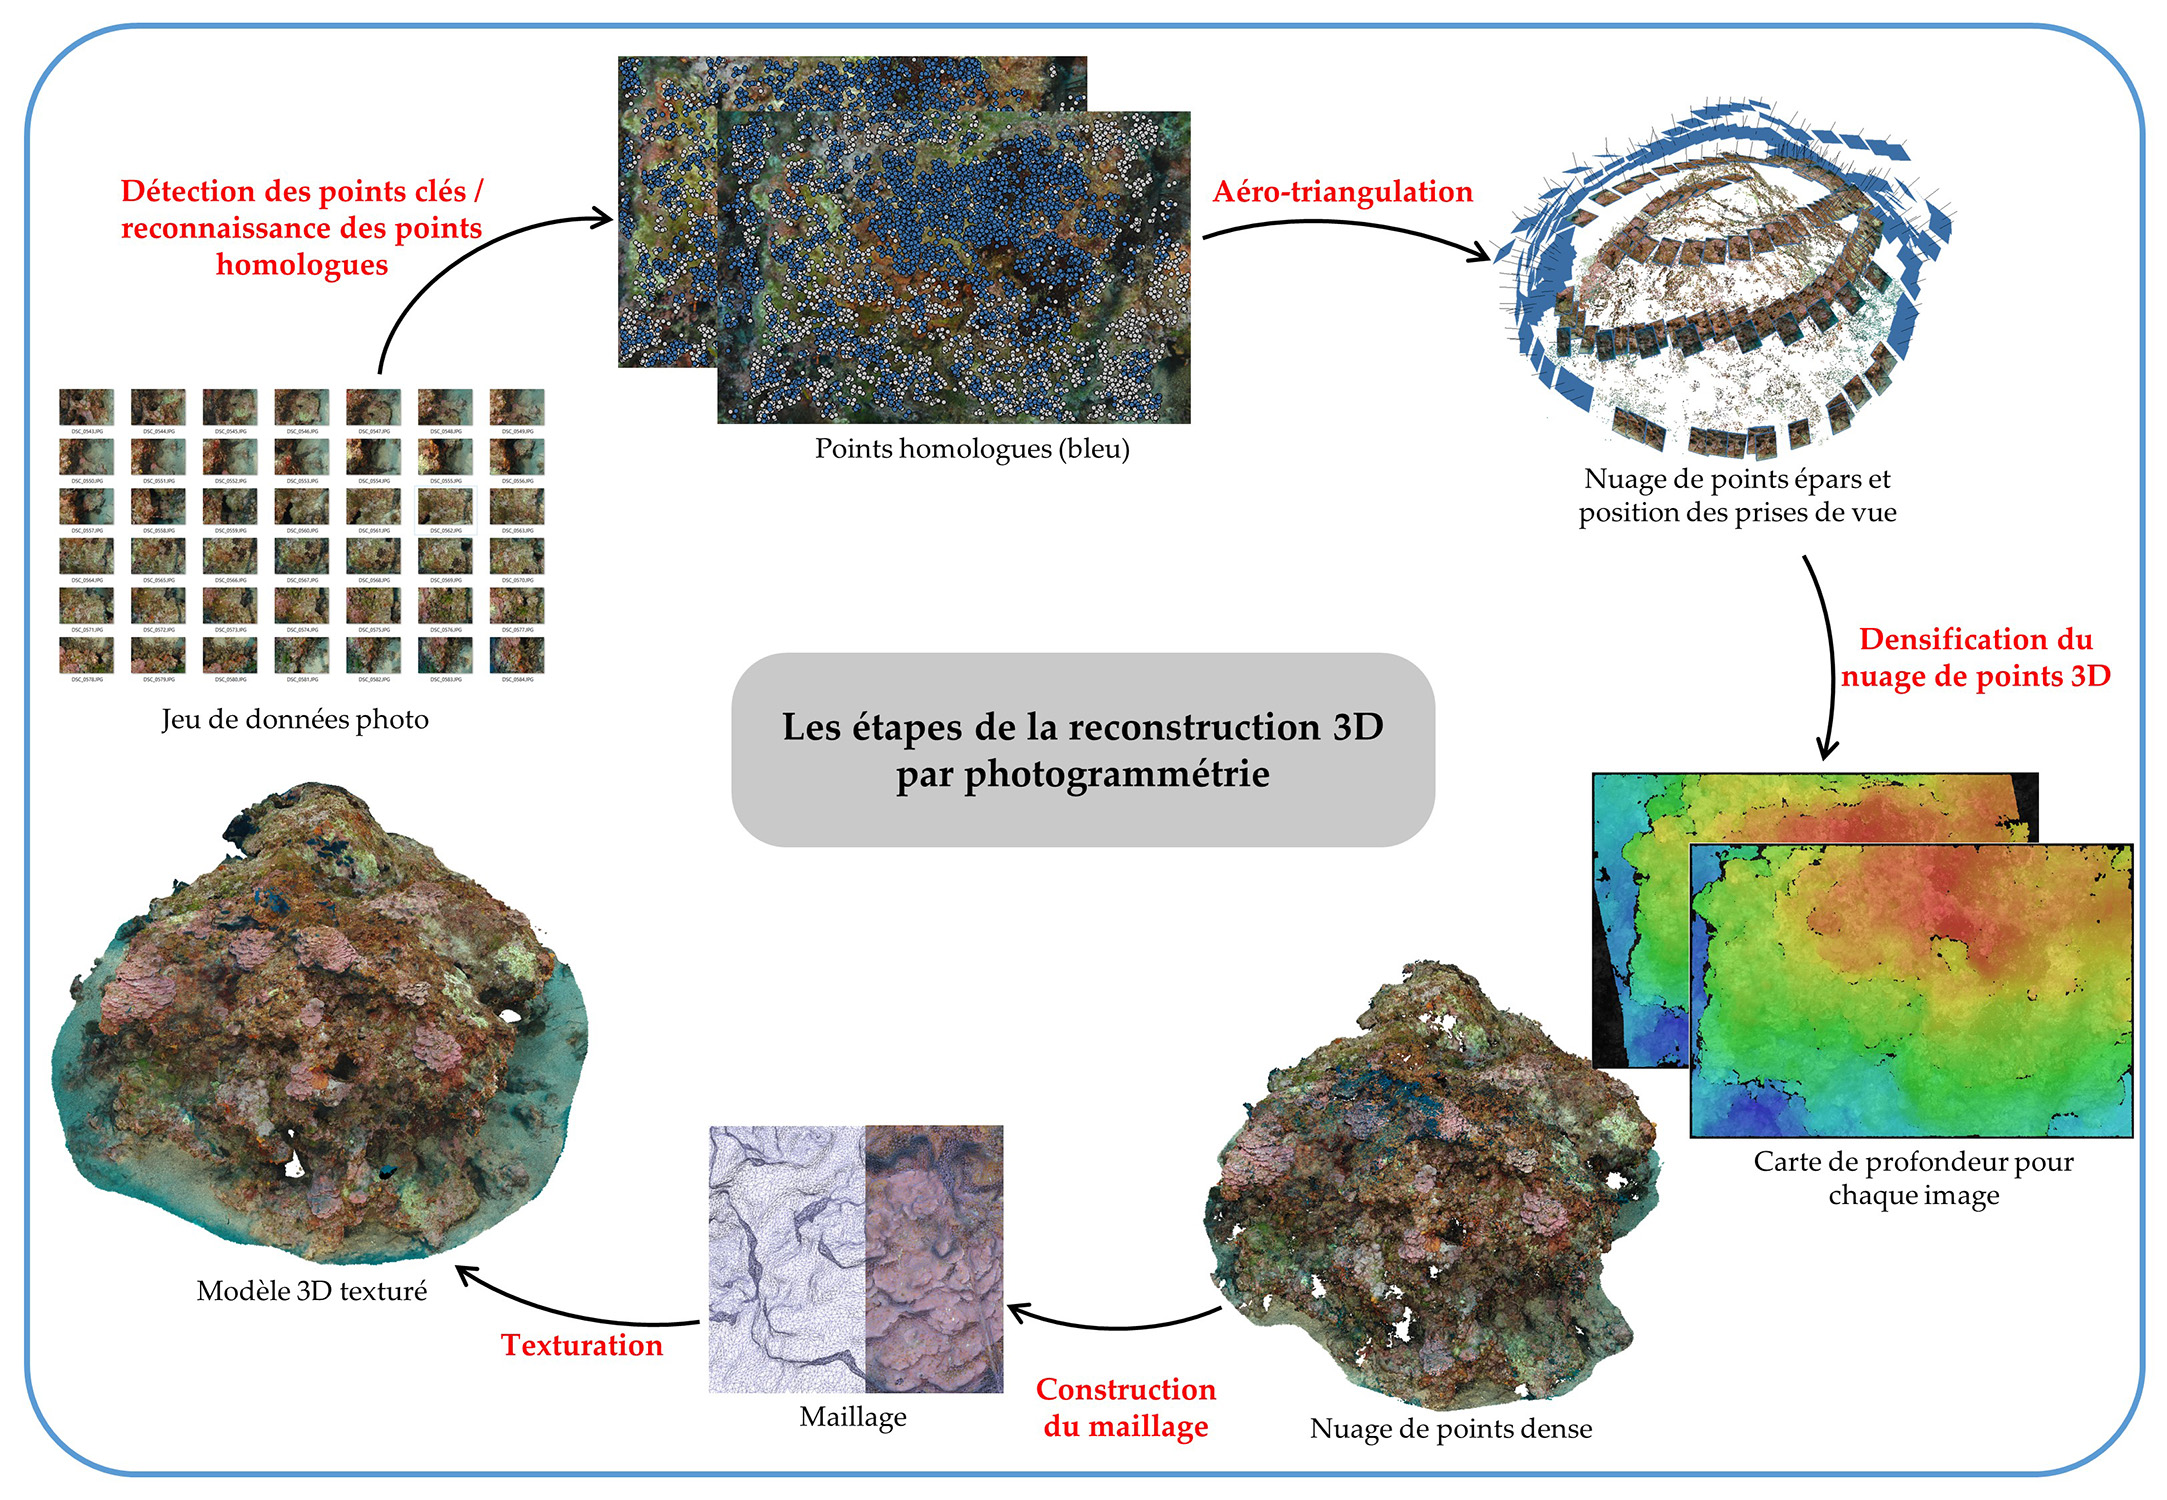
\includegraphics[width=\linewidth,keepaspectratio]{./2_methodes/encart_PG}
		\caption[Les étapes de la reconstruction 3D par photogrammétrie]{Les étapes de la reconstruction 3D par photogrammétrie.}
	\label{figure_methodo8}
\end{center}
\end{figure}
\end{sidewaysfigure}

\subsubsection{Détection des points d’intérêt (« keypoints »)}

L’ensemble des images est d’abord traité à l’aide d’un filtre afin de détecter un grand nombre de points d’intérêt sur l’image, i.e. des candidats susceptibles d’être reconnus entre deux images. Ces points clés se distinguent du reste de l’image par leur singularité : ils doivent être différents de leur voisinage, leur détection doit être robuste à de légères variations de luminosité et de contraste, ils doivent être invariants à de petites déformations géométriques, et leur détection doit être précise en X et en Y. Il existe un certain nombre de méthodes permettant de détecter ces points, mais la plus répandue est l’opérateur SIFT (pour « Scale Invariant Feature Transform »; \autoref{figure_methodo9}), car il est robuste à des différences significatives induites par une rotation, un changement d’échelle et des petites différences de perspectives entre images \citep{luhmann_close-range_2014}.

%%%%%%%%%%%%%%%%%%%%%%%%%%%%%%%%%%%%%%%%%%%%%%
%%% Figure methodo9: SIFT détection points %%%
%%%%%%%%%%%%%%%%%%%%%%%%%%%%%%%%%%%%%%%%%%%%%%
\begin{figure}[H]
	\begin{center}
	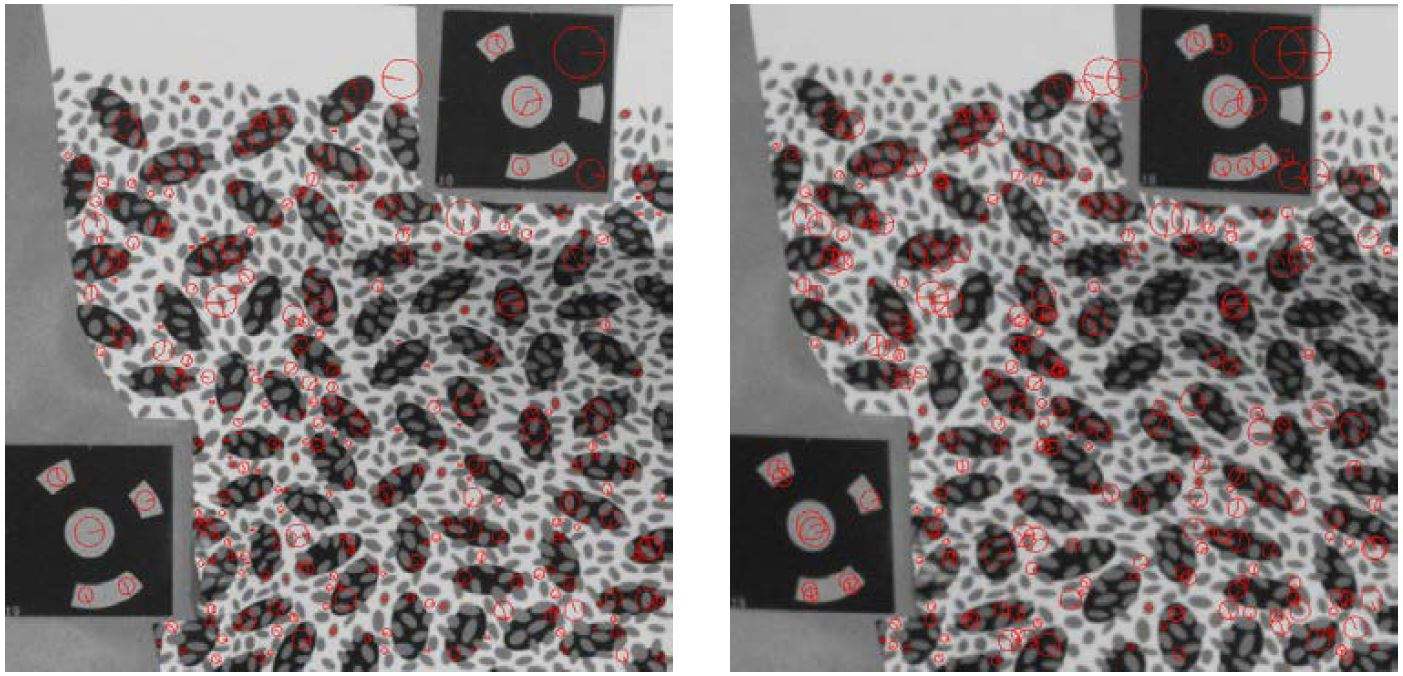
\includegraphics[width=\linewidth,keepaspectratio]{./2_methodes/SIFT_detection_Luhmann2014}
		\caption[Détection de points clés par utilisation de l’opérateur SIFT]{Détection de points clés par utilisation de l’opérateur SIFT \citep{luhmann_close-range_2014}. La taille du cercle indique à quelle échelle le point a été détecté, et la marque indique la direction du gradient dominant.}
	\label{figure_methodo9}
\end{center}
\end{figure}

Par un jeu d’opérations numériques sur l’image entière, l’opérateur SIFT permet donc de rapidement \textbf{détecter les points clés} (coordonnées XY sur l’image) et de calculer un \textbf{vecteur de descripteurs locaux} pour chaque point clé, dont les valeurs sont \textbf{invariantes à la rotation et à l’échelle}. Les descripteurs locaux correspondent à des statistiques de distribution des gradients localement calculés dans une fenêtre de 16 $\times$ 16 pixels autour du point clé. Un certain nombre de points clés sont détectés sur chaque image, en fonction de la texture de l’image (un mur blanc ne contiendra pas ou peu de points, une surface avec une texture riche et nette en contiendra davantage) avec chacun leur vecteur de descripteurs locaux associés.

\subsubsection{Reconnaissance des points homologues (« tie points »)}

Une fois les points clés détectés, il s’agit de réussir à associer les points homologues entre les images en commettant le moins d’erreurs possible, car la précision de la reconstruction 3D en dépend. Pour ce faire, l’algorithme calcule les différences entre les vecteurs de descripteurs de tous les points clés des deux images (ou plus) et associe les points dont les descripteurs sont les plus semblables (ceux dont la différence est minimale) (\autoref{figure_methodo10}). 

%%%%%%%%%%%%%%%%%%%%%%%%%%%%%%%%%%%%%%%%%%%%%%%%%
%%% Figure methodo10: SIFT association points %%%
%%%%%%%%%%%%%%%%%%%%%%%%%%%%%%%%%%%%%%%%%%%%%%%%%
\begin{figure}[H]
	\begin{center}
	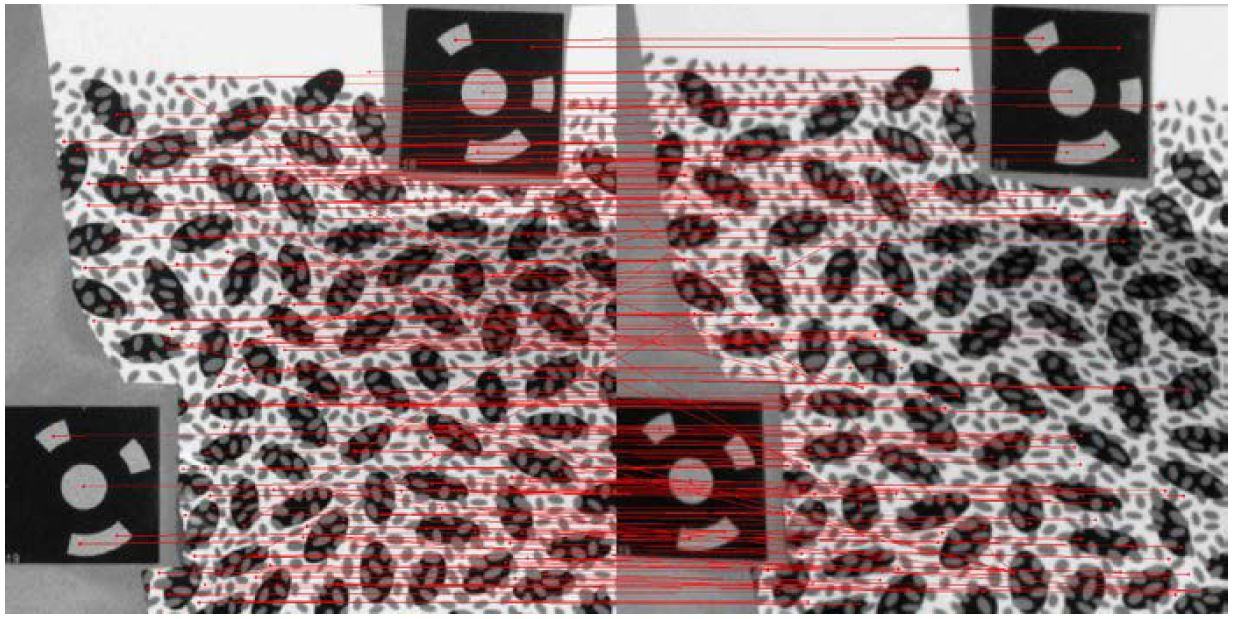
\includegraphics[width=\linewidth,keepaspectratio]{./2_methodes/SIFT_matching_Luhmann2014}
		\caption[Association des points clés détectés avec l’algorithme SIFT]{Association des points clés détectés avec l’algorithme SIFT \citep{luhmann_close-range_2014}.}
	\label{figure_methodo10}
\end{center}
\end{figure}

Cependant, une image contient souvent plusieurs points clés dont les descripteurs sont très semblables, car le même motif apparaît plusieurs fois dans l’image (par exemple : un damier, une grille…). Ceci implique qu’une certaine proportion de ces appariements est erronée, et il est important de réussir à isoler un maximum de mauvaises associations pour ne conserver que des points homologues fiables entre les images et ne pas propager l’erreur. Les erreurs sont détectées à l’aide de l’algorithme RANSAC (pour « RANdom SAmple Consensus », \citep{fischler_random_1981}) qui fonctionne de la manière suivante :

\newpage

\begin{enumerate}
    \item Sélection aléatoire d’un petit nombre de points (nombre minimal suffisant pour estimer les paramètres de l’orientation entre les images)~;
    
    \item Calcul de l’orientation relative des images sur la base de ces points (donc estimation des paramètres d’orientations internes et externes, cf. sous-partie suivante « aéro-triangulation »)~;
    
    \item Parmi les points non sélectionnés, mesure du nombre de points en accord avec l’estimation de l’orientation calculée sur le petit échantillon (avec une marge d’erreur acceptable, par exemple un pixel)~;
    
    \item Répétition des points 1-3 un grand nombre de fois ; le modèle retenu est celui permettant de maximiser le nombre de points en accord avec le modèle. Les couples de points qui s’en écartent trop sont considérés comme de fausses associations.
\end{enumerate}

Cet algorithme permet de supprimer efficacement les faux points homologues, mais le nombre d’itérations nécessaires pour s’assurer de trouver le meilleur modèle augmente avec la proportion de faux points homologues et explose littéralement avec le nombre de paramètres à estimer. Cet algorithme est utilisé dans de nombreux problèmes d’associations d’images (photogrammétrie, assemblages panoramiques, positionnement de robots par image…) et reste efficace tant que le modèle optique à construire n’excède pas une dizaine de paramètres.

\subsubsection{Aéro-triangulation}

\textbf{L’aérotriangulation} correspond au problème de \textbf{positionnement des points 3D} visibles sur une séquence d’images, et à l’estimation des paramètres \textbf{internes} (paramètres de calibration optique de l’appareil photo) et \textbf{externes} (positionnement et rotation des prises de vue). Dans le cas d’une reconstruction à partir de plusieurs images (généralement un grand nombre d’images N), la méthode utilisée est le \textbf{« bundle adjustment »}. Cette méthode permet de simultanément estimer la position et rotation des images ainsi que les positions 3D des points observés, en minimisant l’erreur de reprojection de l’ensemble des points 3D et des images par une approche des moindres carrés \citep{forstner_photogrammetric_2016}. Les inconnues de cette équation sont :

\begin{itemize}
    \item Localisations XYZ des points 3D ($3 \times K$ (points) paramètres)
    
    \item Facteur d’échelle (1 paramètre)
    
    \item Paramètres externes de chaque image (coordonnées $XYZ$ + 3 angles de rotation = 6 paramètres)
    
    \item Paramètres internes linéaires de l’appareil photo (appareil photo et réglages identiques pour tout le jeu de données) :
    
    \begin{itemize}
        \item $F$ : distance focale réelle du système optique
        
        \item $c_x$, $c_y$ : coordonnées d’intersection de l’axe optique principal avec le centre du capteur
        
        \item $b1$, $b2$ : coefficients d’affinité et de cisaillement (i.e. correction de la non-uniformité des échelles sur les axes X et Y)
    \end{itemize}
    
    \item Paramètres internes non linéaires (généralement négligés dans un premier temps) :
    
    \begin{itemize}
        \item $k1$, $k2$, $k3$, $k4$ : coefficients de distorsion radiale
        
        \item $p1$, $p2$, $p3$, $p4$ : coefficients de distorsion tangentielle
    \end{itemize}
\end{itemize}

Le « bundle adjustment » permet donc d’estimer précisément l’ensemble de ces paramètres à partir des points homologues détectés entre les images et de leurs coordonnées XY sur chaque image (voir partie précédente). Par exemple, dans le cas d’un jeu de données composé de 10 000 images (appareil photo et réglages identiques pour tout le jeu de données), 1 000 points par image, chaque point étant visible en moyenne sur 10 images :

\begin{itemize}
    \item \textbf{Nombre d’observations :} 2 (XY) $\times$ 10 000 (images) $\times$ 1 000 (points / image) = 20 000 000 observations
    
    \item \textbf{Nombre d’inconnues :} 1 000 000 (points 3D) $\times$ 3 (XYZ) + 10 000 (images) $\times$ 6 (paramètres externes) + 5 paramètres internes + 1 facteur d’échelle = 1 060 006 paramètres
    
    \item \textbf{Résolution :} nettement plus d’observations que d’inconnues, donc le système d’équations est théoriquement soluble.
\end{itemize}

Le bundle adjustment est statistiquement optimal dans la mesure où il exploite l’ensemble des observations pour l’estimation des paramètres et considère toutes les incertitudes (notamment l’incertitude de localisation des points homologues sur les images). En revanche, cette méthode d’optimisation nécessite une initialisation avec une première paramétrisation grossière : soit par des informations externes (localisation GPS, orientation par une centrale inertielle, calibration optique), soit par l’alignement séquentiel des images pour obtenir un positionnement approximatif. Si chaque point 3D doit apparaître a minima sur deux images pour pouvoir être reconstruit, il faut au moins quatre observations par point pour détecter et identifier une erreur grossière d’appariement (objet répété dans l’espace reconstruit, objet en mouvement…).

\subsubsection{Densification du nuage de points 3D}

A ce stade de la reconstruction, le nuage de points 3D produit par la reconnaissance de points homologues et le bundle adjustment est très peu dense (« sparse point cloud »), car seuls les points saillants qui se distinguent de leur voisinage sur les images ont été détectés comme points d’intérêt et associés entre images. Pour produire un nuage de points dense, capturant un maximum de détail de la scène 3D reconstruite, il est nécessaire d’associer autant que faire se peut chaque pixel d’une image à un pixel d’une autre image (ou de plusieurs images). Afin de réduire l’espace de recherche des points homologues pour chaque pixel, les algorithmes utilisent la « contrainte épipolaire » \citep{forstner_photogrammetric_2016} : à partir de la position relative de deux images, il est possible de définir pour chaque pixel d’une image la ligne épipolaire contenant les seules positions possibles du pixel homologue sur l’autre image (\autoref{figure_methodo11}). Cela permet de réduire l’espace de recherche à une seule dimension et accélère grandement les calculs. L’association des pixels homologues est faite sur la base de descripteurs locaux, de manière similaire à la détection des points homologues durant la phase initiale de la reconstruction.

%%%%%%%%%%%%%%%%%%%%%%%%%%%%%%%%%%%%%%%%%%%
%%% Figure methodo11: Epipolar geometry %%%
%%%%%%%%%%%%%%%%%%%%%%%%%%%%%%%%%%%%%%%%%%%
\begin{figure}[H]
	\begin{center}
	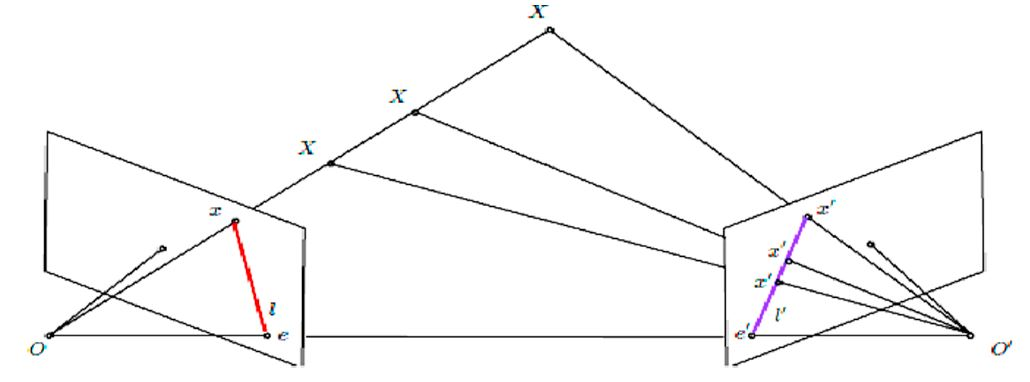
\includegraphics[width=\linewidth,keepaspectratio]{./2_methodes/epipolar_geometry}
		\caption[Illustration de la géométrie épipolaire]{Illustration de la géométrie épipolaire \citep{emmanouil_comparison_2015}. $O$ et $O^\prime$ deux images, $x$ et $x^\prime$ les projections du point $X$ sur les deux images ; $e$ et $e^\prime$ les épipoles de chaque image ; $l$ et $l^\prime$ les lignes épipolaires des deux images.}
	\label{figure_methodo11}
\end{center}
\end{figure}

Pour chaque pixel de chaque image, la distance à l’objet est calculée à partir des associations précédemment faites et de l’orientation relative des images. Il en résulte une carte de profondeur (distance à l’objet en chaque pixel) pour chaque image, à partir desquelles il est possible de déterminer les coordonnées 3D de l’ensemble des pixels pour construire le nuage de points dense. Le résultat est généralement bruité par de mauvaises associations ou de légères erreurs de positionnement, mais des algorithmes permettent de filtrer les points isolés ayant de grandes chances d’être des artefacts de reconstruction.

\subsubsection{Construction du maillage}

Le nuage de points dense est ensuite drapé par une surface 3D (i.e. maillage ou « mesh ») sur laquelle pourra être projetée la texture issue des images. L’objectif est de définir une surface 3D continue qui passe au plus proche de l’ensemble des points du nuage de points dense, en reproduisant le plus fidèlement les détails de la scène sans conserver les petits artefacts de reconstruction du nuage de points dense. Plusieurs algorithmes existent, mais le plus connu et utilisé est certainement l’algorithme de reconstruction de surface de Poisson \citep{kazhdan_poisson_2006}. Le maillage ainsi produit est constitué de faces et de sommets qui interconnectent les faces entre elles. Les faces sont généralement triangulaires mais il est aussi possible de définir des faces quadratiques (parallélépipèdes).

\subsubsection{Application d’une texture}

La texture correspond aux motifs observés sur une surface et dus aux variations de structure et de couleur dans un voisinage restreint. Cette apparence de l’objet est le résultat des propriétés de réflexion du matériau ainsi que des caractéristiques géométriques locales de la surface. Si cette étape n’est pas indispensable au processus de reconstruction 3D, l’application d’une texture au maillage permet de donner une apparence réaliste aux reconstructions 3D et de mieux visualiser l’objet reconstruit \citep{luhmann_close-range_2014}. Il existe plusieurs manières de procéder, mais bien souvent la texture associée à un chaque face du maillage est extraite de l’image qui la représente le mieux (i.e. l’image la plus orthogonale à la face, la plus proche, la mieux exposée…).

\subsection{Spécificités du milieu marin}

Alors que la démocratisation des images satellites et des drones permet aujourd’hui d’avoir accès à des images aériennes de grande qualité et le plus souvent géoréférencées, une grande partie du milieu marin reste inobservable de cette manière. Dans le cas des drones, des programmes de gestion de plan de vol permettent de réaliser des acquisitions photogrammétriques parfaitement maîtrisées (ex. : Fligh Plan de la marque Parrot) et ainsi maîtriser la qualité des reconstructions, mais le milieu sous-marin étant un milieu contraignant, une fois sous la surface de l’eau, tout devient plus complexe : positionnement, visibilité…

\subsubsection{Géoréférencement indisponible}

Le signal GPS ne fonctionne pas sous l’eau, ce qui rend impossible tout positionnement absolu des images. Ce problème est bien connu des roboticiens qui travaillent sur le développement de robots autonomes. La seule manière d’obtenir une position sous l’eau est par positionnement relatif à un objet en surface de position absolue connue, ou encore par intégration des mouvements de l’objet à positionner depuis sa dernière position absolue en surface. Cette dernière option, qui utilise une centrale inertielle (contenant des accéléromètres), rencontre d’importants problèmes de dérive avec le temps, et les solutions les plus précises sont généralement très coûteuses et peu compactes.

Pourtant, le positionnement a priori des images par l’enregistrement simultané du signal GPS permet d’améliorer la qualité et la rapidité de l’aérotriangulation. En effet, les calculs peuvent souffrir d’une dérive due à l’accumulation de petites erreurs de positionnement relatif dans le cas de gros jeux de données, et l’utilisation du positionnement GPS permet de contraindre cette dérive et d’améliorer l’ajustement \citep{lhuillier_incremental_2012}. Par ailleurs, le positionnement GPS des images de la séquence permet de géoréférencer le modèle 3D produit, et donc de le mettre automatiquement à l’échelle, correctement positionné et orienté. Sans positions absolues des images, il est indispensable d’utiliser a minima des points de contrôle sur la scène afin de mettre le modèle à l’échelle et au besoin d’orienter et géoréférencer le modèle a posteriori.

\subsubsection{L’absorption lumineuse}

Bien que translucide, l’eau est 1000 fois plus dense que l’air et absorbe une grande partie de l’énergie lumineuse qui la traverse \citep{wozniak_light_2007}. Cette absorption est d’autant plus forte que la couche d’eau traversée est grande, et il ne reste plus guère de lumière passé 100 m de fond. Par ailleurs, l’absorption n’est pas homogène sur tout le spectre visible, et les rouges sont absorbés dès 20 m de fond. L’utilisation de la photogrammétrie en milieu sous-marin implique donc de se limiter aux petits fonds pour bénéficier d’un éclairement naturel suffisant, ou impose l’utilisation d’éclairages artificiels qui posent d’autres problèmes potentiels : éclairement hétérogène selon la profondeur dans l’image et pouvant perturber les algorithmes de reconstruction, ombres portées masquant certaines parties de l’image, nécessité d’une plus grande proximité à l’objet…

\subsubsection{La réfraction}

La réalisation de photos sous-marines implique l’utilisation d’un caisson étanche et donc d’une optique externe à travers laquelle la lumière pénètre dans le caisson. Les rayons lumineux qui passent de l’eau à l’air en traversant cette optique subissent une réfraction et sont déviés avant d’atteindre l’objectif de l’appareil photo et peuvent affecter le processus de reconstruction photogrammétrique \citep{telem_photogrammetric_2010}. En effet, cette réfraction cause des déformations \\géométriques et une réduction du champ de vision, c’est pourquoi il est courant d’utiliser un dôme hémisphérique plutôt qu’un dôme plan afin de compenser la réfraction et d’améliorer la qualité des reconstructions 3D (\autoref{figure_methodo12}) \citep{menna_optical_2017}. Si le système optique composé de l’objectif et de l’optique externe sous l’eau n’est pas équivalent à l’appareil l’objectif seul à l’air libre, il a été démontré que les déformations optiques résiduelles peuvent être absorbées et corrigées par l’auto-calibration réalisée pendant la phase d’aérotriangulation \citep{shortis_calibration_2015}.

%%%%%%%%%%%%%%%%%%%%%%%%%%%%%%%%%%%%
%%% Figure methodo12: Réfraction %%%
%%%%%%%%%%%%%%%%%%%%%%%%%%%%%%%%%%%%
\begin{figure}[H]
	\begin{center}
	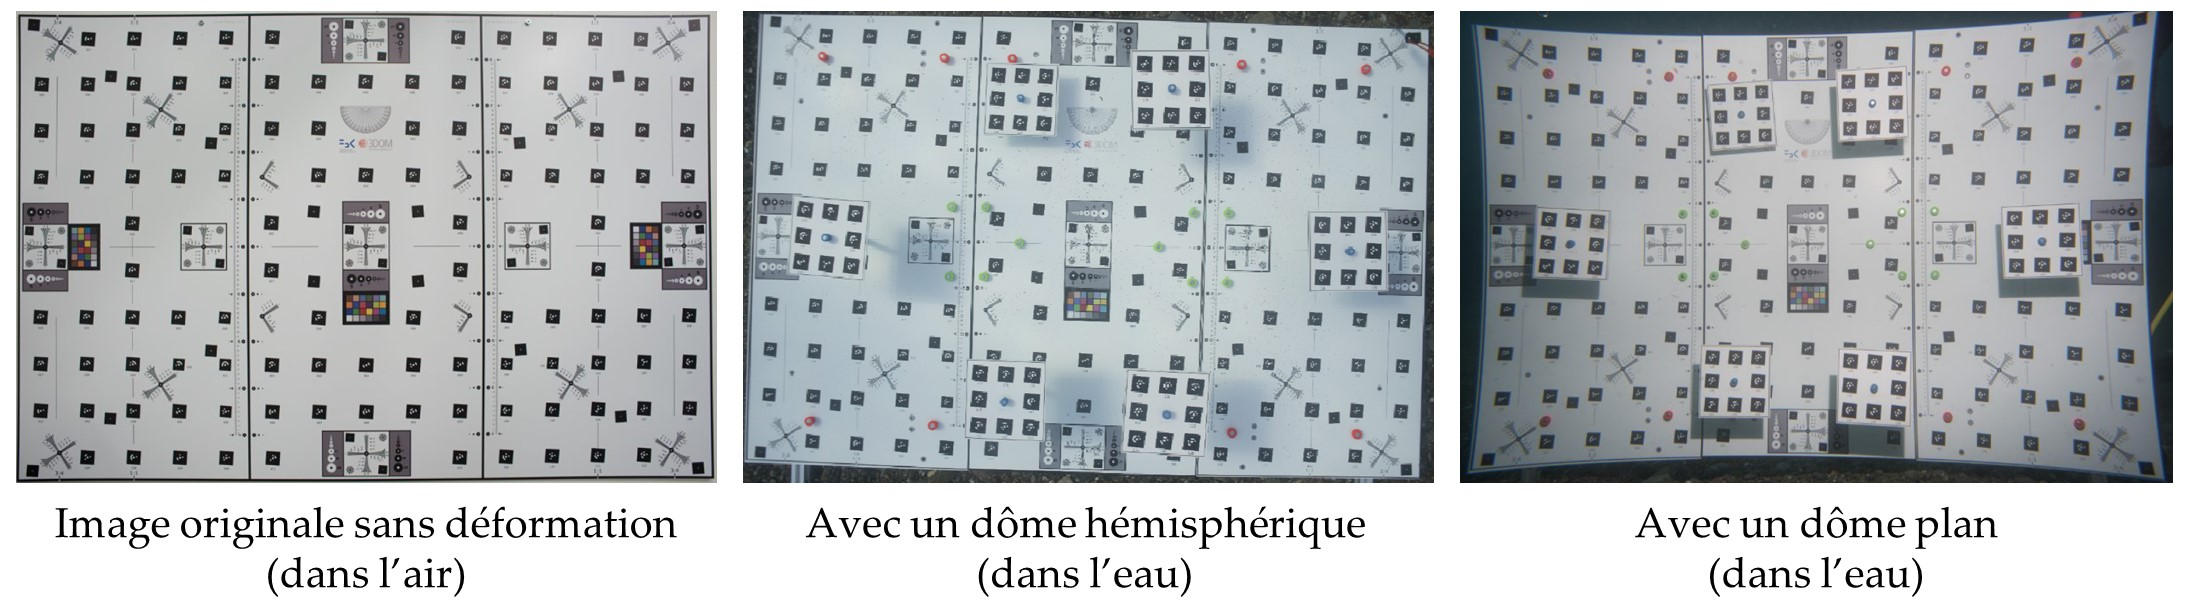
\includegraphics[width=\linewidth,keepaspectratio]{./2_methodes/refraction_Menna2017}
		\caption[Déformations optiques avec un dôme hémisphérique ou un dôme plan]{Déformations optiques avec un dôme hémisphérique ou un dôme plan (adapté de \citet{menna_optical_2017}).}
	\label{figure_methodo12}
\end{center}
\end{figure}

\subsubsection{Présence d’objets mobiles sur la scène}

Les habitats sous-marins sont peuplés d’espèces fixées soumises aux courants marins (plantes marines, algues, gorgones…) et d’espèces mobiles comme les poissons. S’ils occupent une part trop importante de l’image, ces objets en mouvement peuvent largement perturber le processus de reconstruction, qui repose à la base sur la reconnaissance de points homologues pour calculer le positionnement des images et les coordonnées 3D des points de la scène. C’est le cas particulièrement sur les récifs coralligènes où l’on rencontre régulièrement d’abondantes populations de poissons (\autoref{figure_methodo13}).

%%%%%%%%%%%%%%%%%%%%%%%%%%%%%%%%%%%%%%%%%
%%% Figure methodo13: Espèces mobiles %%%
%%%%%%%%%%%%%%%%%%%%%%%%%%%%%%%%%%%%%%%%%
\begin{figure}[H]
	\begin{center}
	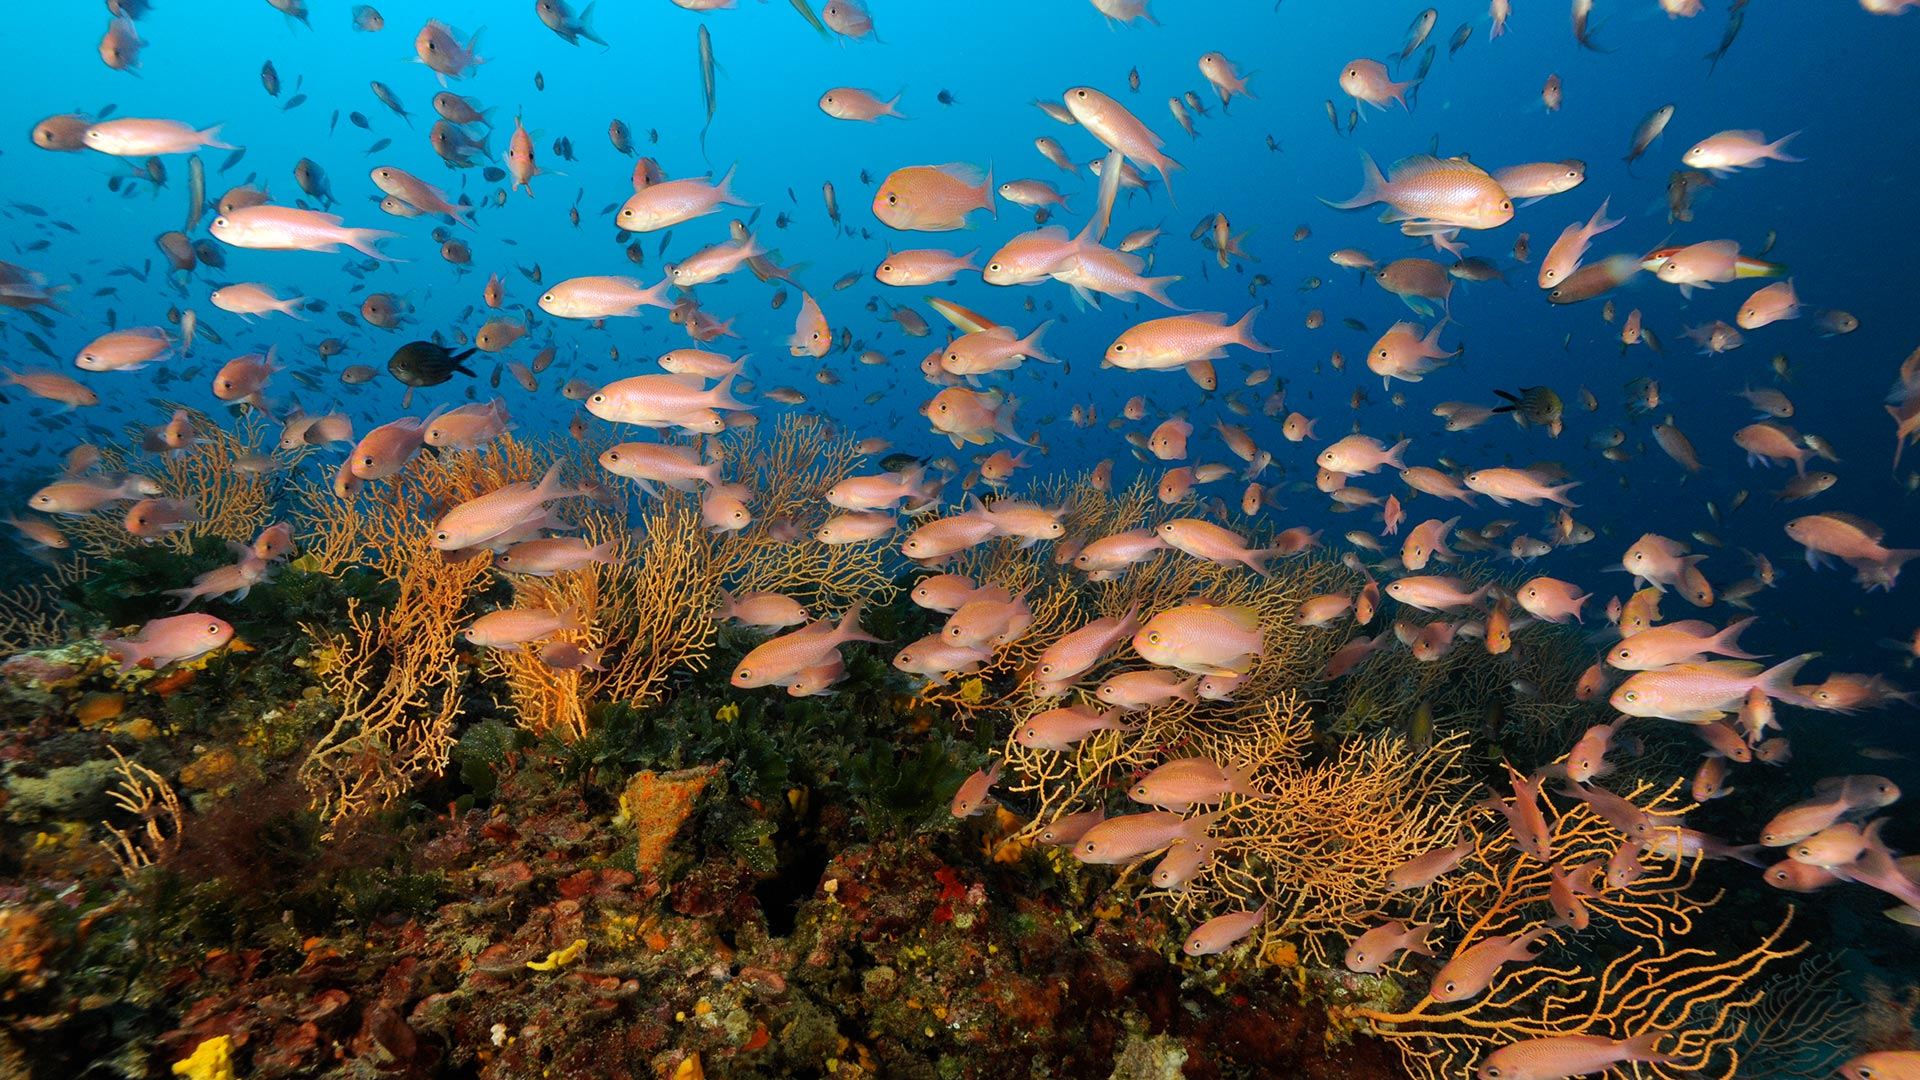
\includegraphics[width=\linewidth,keepaspectratio]{./2_methodes/especes_mobiles}
		\caption[Illustration du problème des espèces mobiles sur les images sous-marines]{Illustration du problème des espèces mobiles sur les images sous-marines. Ici de nombreux barbiers communs (\textit{Anthias anthias}) sur un récif coralligène (\textit{©Andromède océanologie}).}
	\label{figure_methodo13}
\end{center}
\end{figure}

\newpage

\subsection{La photogrammétrie en pratique}

\subsubsection{Acquisition des images}

L’acquisition des images est une étape clé pour une reproduction de qualité. L’objectif est d’assurer un recouvrement suffisant entre les images pour permettre leur bon alignement dans l’espace, avec des transformations (translation, rotation, homothétie) entre deux images que les algorithmes sauront interpréter. Il est en général recommandé de maintenir un minimum de 80 \% de recouvrement entre deux images successives (80 \% des deux images recouvrent une partie commune de l’objet) et 60 \% de recouvrement latéral (i.e. entre deux « bandes » d’images) \citep{agisoft_agisoft_2018-1} pour assurer le bon alignement des images dans l’espace. Il est bien entendu possible de recouvrir plus encore, mais un trop fort taux de recouvrement risque d’affecter significativement le temps de calcul et les besoins en mémoire, qui augmentent exponentiellement avec le nombre d’images \citep{agisoft_agisoft_2018}. Par ailleurs, la trajectoire et l’orientation des images sont importantes : il est recommandé de suivre une trajectoire localement parallèle à la surface de l’objet, et une orientation de la prise de vue perpendiculaire à celle-ci (\autoref{figure_methodo14}). Concernant la distance à l’objet, il faut respecter la règle « aussi loin que nécessaire, mais aussi près que possible » \citep{linder_digital_2016}. Il est donc important d’adapter le protocole d’acquisition à chaque type d’objet en fonction de sa forme et de la qualité de reconstruction requise.

%%%%%%%%%%%%%%%%%%%%%%%%%%%%%%%%%%%%%%%%%%
%%% Figure methodo14: Prises de vue PG %%%
%%%%%%%%%%%%%%%%%%%%%%%%%%%%%%%%%%%%%%%%%%
\begin{figure}[H]
	\begin{center}
	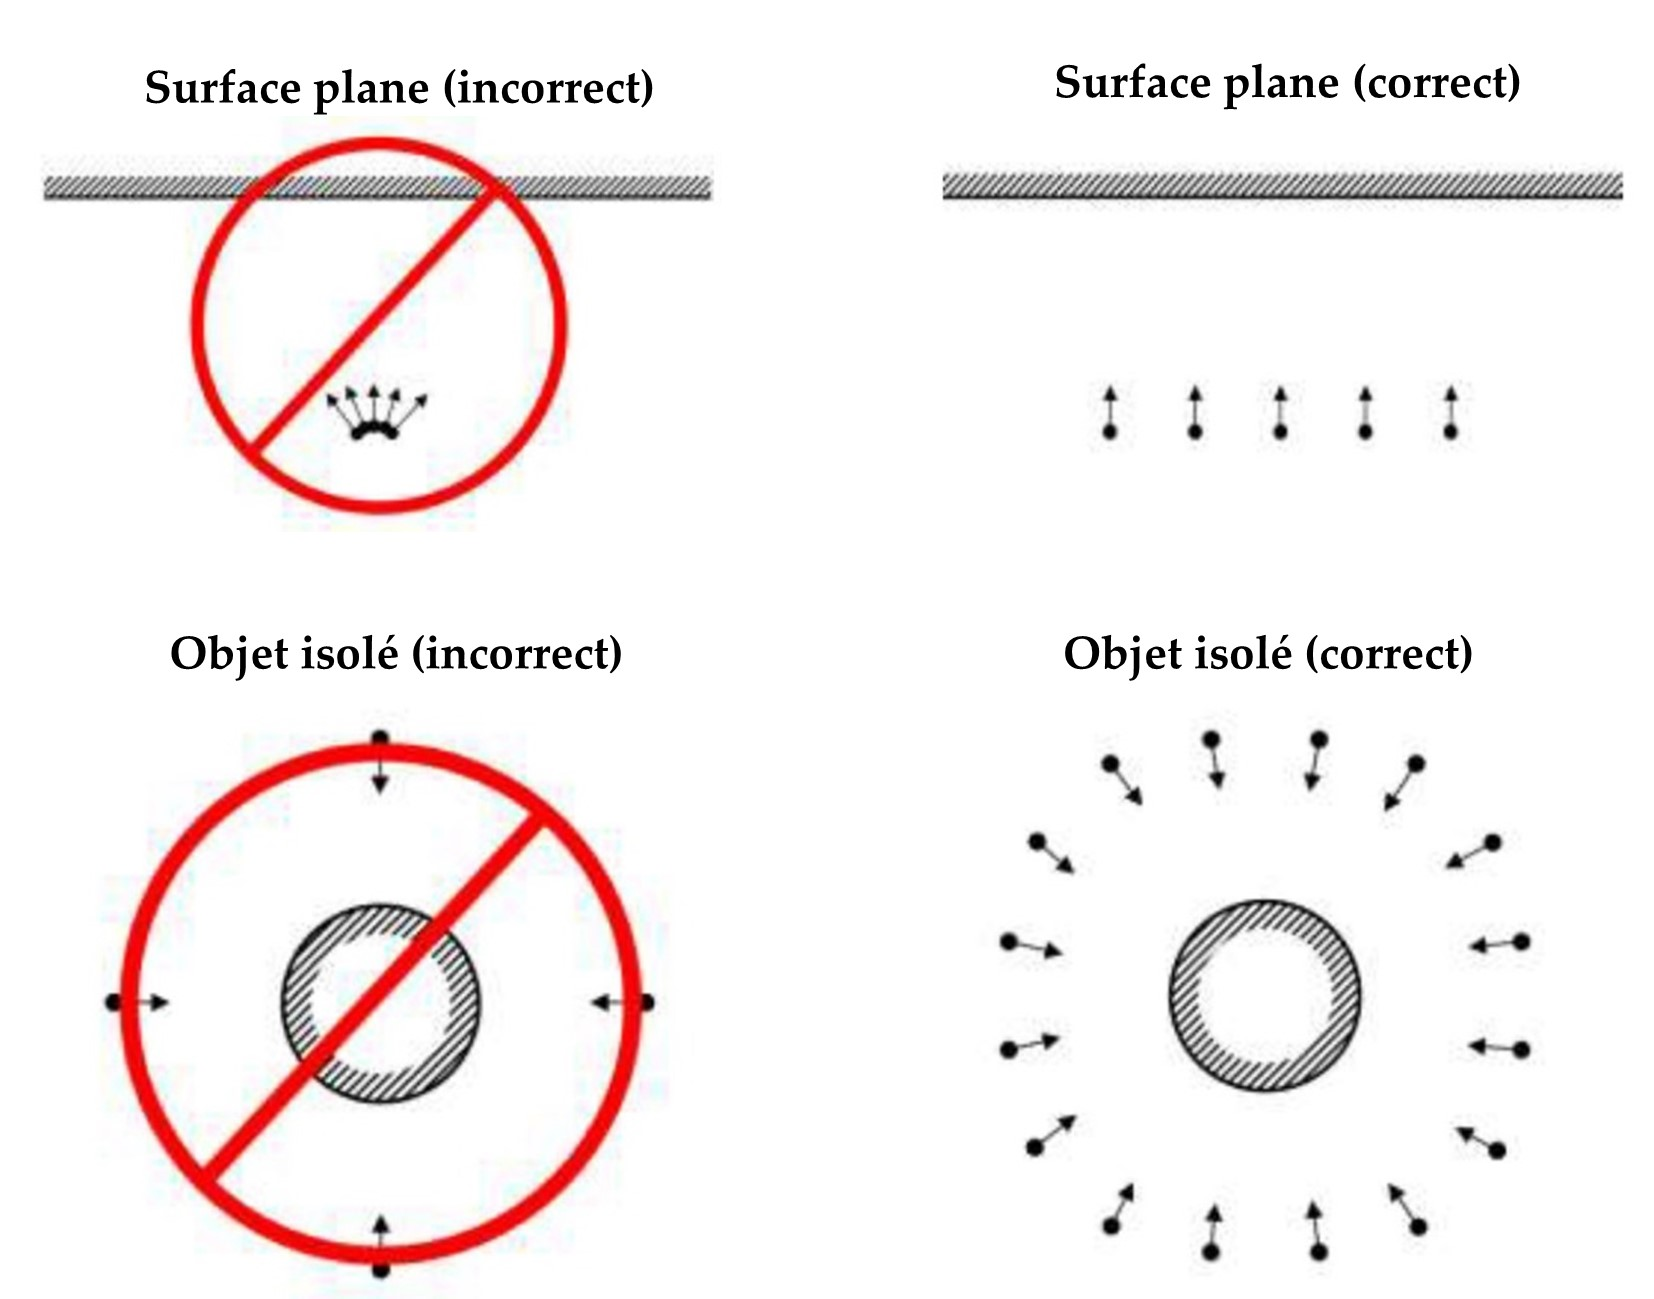
\includegraphics[width=0.7\linewidth,keepaspectratio]{./2_methodes/acquisition_PG}
		\caption[Recommandations de prises de vue pour une reconstruction 3D par photogrammétrie]{Recommandations de prises de vue pour une reconstruction 3D par photogrammétrie (adapté de \citet{agisoft_useful_2018}).}
	\label{figure_methodo14}
\end{center}
\end{figure}

La trajectoire d’acquisition dépend elle aussi de la nature et de la forme de l’objet ou de la scène à numériser. Dans le cas d’une scène relativement plane, il convient de survoler la zone en réalisant des transects parallèles, et dans le cas d’un objet plus complexe, il peut être nécessaire de suivre les courbes de niveau de l’objet en restant localement orthogonal à la surface de l’objet (\autoref{figure_methodo15}).

%%%%%%%%%%%%%%%%%%%%%%%%%%%%%%%%%%%%%%%%
%%% Figure methodo15: Trajectoire PG %%%
%%%%%%%%%%%%%%%%%%%%%%%%%%%%%%%%%%%%%%%%
\begin{figure}[H]
	\begin{center}
	\includegraphics[width=\linewidth,keepaspectratio]{./2_methodes/trajectoire_PG}
		\caption[Exemples de trajectoires d’acquisition en fonction de la morphologie de l’objet d’étude]{Exemples de trajectoires d’acquisition en fonction de la morphologie de l’objet d’étude. À gauche : un herbier de posidonie ; à droite : un pic rocheux vertical.}
	\label{figure_methodo15}
\end{center}
\end{figure}

\subsubsection{Utilisation de points de contrôle et barres d’échelle}

L’utilisation de points de contrôle, généralement matérialisés par des marqueurs codés de coordonnées connues et automatiquement détectés par un filtre (voir exemple de marqueur \autoref{figure_methodo16}), permet de faire le lien entre le système de coordonnées arbitraire du modèle 3D après reconstruction et le système de coordonnées réel de la scène capturée \citep{forstner_photogrammetric_2016}. Chacun de ces marqueurs codés est reconnu et identifié, ce qui permet d’affecter automatiquement leurs coordonnées renseignées dans un tableau de données et facilite le géoréférencement. À défaut d’avoir à disposition les coordonnées absolues de ces marqueurs, comme c’est a priori le cas sous l’eau, il est possible de se servir des relations géographiques entre marqueurs afin de mettre à l’échelle le modèle via une barre d’échelle (distance connue entre deux marqueurs), ou même de l’orienter grâce à un référentiel local du plan XY défini par un minimum de 3 marqueurs (\autoref{figure_methodo16}).

%%%%%%%%%%%%%%%%%%%%%%%%%%%%%%%%%%%%%%%%%%%%%%%%%%%%%%
%%% Figure methodo16: Points de contrôle cibles PG %%%
%%%%%%%%%%%%%%%%%%%%%%%%%%%%%%%%%%%%%%%%%%%%%%%%%%%%%%
\begin{figure}[H]
	\begin{center}
	\includegraphics[width=\linewidth,keepaspectratio]{./2_methodes/marqueurs}
		\caption[Exemples de marqueurs codés utilisés par le logiciel Agisoft PhotoScan]{Exemples de marqueurs codés utilisés par le logiciel Agisoft PhotoScan. À gauche : les marqueurs codés 1-2-3-4 ; à droite : référentiel local défini par quatre marqueurs aux quatre cardinales.}
	\label{figure_methodo16}
\end{center}
\end{figure}

\subsubsection{Chaîne de traitement avec le logiciel Agisoft PhotoScan}

Les algorithmes utilisés pour l’analyse des images et la reconstruction 3D par photogrammétrie sont aujourd’hui bien connus, et de nombreux logiciels libres ou payants proposent des solutions intégrées pour utiliser ces algorithmes \citep{ioannides_benchmarking_2016}. Pour autant, toutes ces solutions logicielles ne sont pas équivalentes en précision, en robustesse, en coût, en facilité de mise en œuvre et de personnalisation des traitements. L’une d’entre elles, Agisoft PhotoScan \citep{agisoft_agisoft_2018-1}, est largement répandue et appréciée de la communauté scientifique \citep{figueira_accuracy_2015, lavy_quick_2015, burns_assessing_2016, guo_accuracy_2016, bryson_characterization_2017, casella_mapping_2017, mizuno_simple_2017, raczynski_accuracy_2017, raoult_how_2017, collin_very_2018, royer_photogrammetric_2018, ventura_mapping_2018}. En effet, PhotoScan est :

\begin{itemize}
    \item \textbf{Robuste :} il n’échoue presque jamais \citep{ioannides_benchmarking_2016} ;
    
    \item \textbf{Précis :} faibles distances entre surface réelle et reconstruite ;
    
    \item \textbf{Son coût est raisonnable :} 180 – 500 € en version académique ;
    
    \item \textbf{Intuitif :} utilisable en « clic-bouton » ;
    
    \item \textbf{Personnalisable :} grâce à une interface Python permettant de scripter des tâches complexes et d’accéder à tous les objets produits au cours du traitement.
\end{itemize}

L’ensemble des traitements photogrammétriques détaillés dans ce travail de thèse sont réalisés avec le logiciel Agisoft PhotoScan v1.4 \citep{agisoft_agisoft_2018-1}. Ci-dessous le détail des différentes étapes nécessaires à la reconstruction 3D, avec les différents paramètres à renseigner et leur signification.

\paragraph{Aligner les images}

Cette étape inclut la détection de points clés, la reconnaissance des points homologues et l’aérotriangulation des images (voir section 2.2). Elle utilise plusieurs paramètres :

\begin{itemize}
    \item \textbf{Précision de l’alignement :} plus elle augmente, meilleur est le positionnement des images, mais plus le temps de calcul est long. Lorsque l’utilisateur choisit « haute précision », les images sont traitées dans leur résolution originale. Pour chaque niveau de dégradation de la précision (i.e. « moyenne », « faible », « très faible »), la résolution originale est dégradée par un facteur 2 en X et en Y, donc le nombre de pixels de l’image est divisé par 4 ;
    
    \item \textbf{Présélection des paires d’images :} afin de réduire le temps de calcul pour les gros jeux de données, il est possible de réaliser un préalignement imprécis des images se chevauchant ou dont les coordonnées sont renseignées ;
    
    \item \textbf{Nombre maximal de points clés :} permet de contrôler le nombre de points clés détectés par les algorithmes, afin de se limiter aux points les plus fiables ;
    
    \item \textbf{Nombre maximal de points homologues :} permet de contrôler le nombre maximal de points homologues entre deux images et de réduire les erreurs en se limitant aux points clés les plus semblables entre deux images ;
    
    \item \textbf{Ajustement variable du modèle de correction optique :} autorise PhotoScan à choisir automatiquement les paramètres optiques à estimer durant la phase d’alignement. De base, seuls les paramètres suivants sont calculés : $F$, $c_x$, $c_y$, $k1$, $k2$, $k3$, $p1$ et $p2$ (voir section 2.2.3).
\end{itemize}

\paragraph{Optimiser l’alignement}

Durant la première étape, PhotoScan reconnaît les points homologues entre les différentes images et procède à l’aérotriangulation tout en estimant les paramètres optiques de l’appareil photo. Quoique potentiellement déjà satisfaisant, ce premier résultat contient généralement des erreurs associées à des points homologues imprécis ou associés à tort malgré le filtrage par l’algorithme RANSAC (voir section 2.2). Ces erreurs peuvent affecter l’estimation des paramètres optiques et l’orientation interne et externe des images, diminuant ainsi la qualité globale de la reconstruction. C’est pourquoi il est recommandé d’optimiser l’alignement de manière itérative en supprimant les points les moins précis du nuage de points épars (« sparse cloud » : ensemble des points homologues 3D), et en affinant l’estimation des paramètres en se basant sur ce sous-échantillon du nuage de points initial.


\paragraph{Construire un nuage dense}

Une fois le positionnement des images et les corrections optiques précisément estimés, PhotoScan calcule pour chaque image une carte de profondeur (« depth map ») correspondant à la distance entre l’appareil photo et la surface numérisée, en chaque pixel de l’image. PhotoScan combine ensuite l’ensemble de ces cartes de profondeur sous forme d’un nuage de points dense. Cette étape, la plus gourmande en ressources (notamment GPU), nécessite de choisir plusieurs paramètres :

\begin{itemize}
    \item \textbf{Qualité de la reconstruction :} plus elle augmente, meilleure est la qualité de la reconstruction, mais plus le temps de calcul est long. De façon similaire à l’alignement des images, lorsque l’utilisateur choisi « \underline{très} haute précision », les images sont traitées dans leur résolution originale. Pour chaque niveau de dégradation de la précision (i.e. « haute », « moyenne », « faible », « très faible »), la résolution originale est dégradée par un facteur 2 en X et en Y, donc le nombre de pixels de l’image est divisé par 4. Pour une qualité « moyenne », les cartes de profondeurs produites ont une résolution divisée par 4 en X et en Y, soit 16 fois moins de pixels que l’image originale ;
    
    \item \textbf{Filtrage des profondeurs :} à cause d’accumulation d’erreurs, certains points du nuage dense correspondent à des artefacts de reconstruction. PhotoScan possède des algorithmes permettant de filtrer ces points et de les éliminer automatiquement. Ce paramètre correspond au niveau de filtration (aucun, léger, moyen ou agressif) et dépend notamment du niveau de détail souhaité pour le rendu. Dans le cas de modèles contenant beaucoup de détail, il est recommandé d’utiliser un filtrage léger ;
    
    \item \textbf{Réutilisation des cartes de profondeur :} si les cartes de profondeurs ont été calculées une première fois et stockées, ce paramètre permet d’autoriser leur réutilisation (à condition qu’elles correspondent aux mêmes paramètres de qualité de reconstruction et niveau de filtrage). Si l’utilisateur répond « non », les cartes de profondeur seront recalculées ;
    
    \item \textbf{Calculer la couleur des points :} si « oui », PhotoScan détermine une couleur pour chaque point du nuage dense. 
\end{itemize}

\paragraph{Construire un maillage}

Sur la base d’un nuage de points, PhotoScan peut construire un maillage triangulaire 3D. Cette étape nécessite de renseigner les paramètres suivants :

\begin{itemize}
    \item \textbf{Données sources :} nuage épars ou nuage dense. Si l’objectif est d’obtenir une reconstruction 3D fine, choisir « nuage dense ». Si la finalité est la production d’une orthomosaïque sur une surface relativement plane, le nuage épars peut suffire (auquel cas il est inutile de produire le nuage dense) ;
    
    \item \textbf{Type de surface :} « arbitraire » permet de reconstruire n’importe quel type de surface 3D y compris des objets fermés, « champ de hauteur » est optimisé pour les surfaces planes (2,5D) ;
    
    \item \textbf{Nombre de faces :} nombre de triangles composant le maillage final, proportionnel au nombre de points du nuage en entrée : « haut » (1 / 5e), « moyen » (1 / 15e) ou « bas » (1 / 45e). Il est également possible de renseigner un nombre personnalisé de faces ; 
    
    \item \textbf{Interpolation :} permet d’autoriser ou non PhotoScan à interpoler entre les points du nuage en entrée pour « boucher les petits trous » dans la surface reconstruite ;
    
    \item \textbf{Calculer les couleurs des sommets :} si la donnée source contient une information de couleur, elle peut être transférée à chaque sommet du maillage généré.
\end{itemize}

\paragraph{Appliquer une texture}

La texture d’un modèle 3D correspond à une mosaïque de portions d’images brutes, drapée sur le maillage pour lui donner un aspect plus réaliste et résolu. Cette étape nécessite de renseigner les paramètres suivants :

\begin{itemize}
    \item •	Mode de mappage : ce paramètre conditionne la manière dont la texture est stockée, afin de minimiser sa taille tout en maximisant la qualité du rendu visuel. Ce paramètre dépend de l’objet d’étude : « générique » dans le cas d’une surface 3D arbitraire complexe, mais il existe d’autres modes permettant de compacter la texture notamment dans le cas d’acquisitions aériennes plus planes (« orthophoto ajustée », « orthophoto ») ou encore des cas particuliers (« sphérique », « photo unique ») ;
    
    \item •	Mode de fusion : détermine comment les pixels des différentes images sont combinés lors de la production de la texture :
    
    \begin{itemize}
        \item \textbf{Mosaïque :} afin de limiter les effets visuels de jointure entre images, la texture générale est déterminée par une moyenne pondérée entre les différentes photos, et la texture des plus petits détails est extraite d’une seule image (l’image la plus orthogonale à la surface 3D en chaque point) ;
        
        \item \textbf{Moyenne :} moyenne pondérée des valeurs des pixels de toutes les images ;
        
        \item \textbf{Intensité max :} l’image possédant l’intensité maximale pour le pixel considéré est choisie ;
        
        \item \textbf{Intensité min :} l’image possédant l’intensité minimale pour le pixel considéré est choisie ;
        
        \item \textbf{Désactivé :} dans ce cas, aucune fusion n’est réalisée et l’ensemble de la texture est déterminée comme pour les plus petits détails en mode « mosaïque » ;
    \end{itemize}
    
    \item \textbf{Taille de la texture :} hauteur et largeur de l’atlas de texture produit (image) ;
    
    \item \textbf{Nombre de textures :} permet d’exporter la texture en plusieurs fichiers d’images. Dans le cas d’un gros modèle et d’une texture très résolue, il est préférable d’exporter plusieurs fichiers afin de limiter les besoins en mémoire vive ;
    
    \item \textbf{Remplissage des trous :} permet d’interpoler la texture dans les zones de petites ombres portées dans le cas de surfaces complexes ;
    
    \item \textbf{Activer le filtre fantôme :} en cas de présence de fines structures ou d’objets mobiles sur la scène, cette option permet de les détecter sur les images pour éviter ces impressions « fantômes » sur la texture finale.
\end{itemize}

\paragraph{Produire une orthomosaïque}

Cette étape est optionnelle et permet de reconstruire une image aérienne orthorectifiée de la scène, elle nécessite de renseigner les paramètres suivants :

\begin{itemize}
    \item \textbf{Résolution :} taille d’un pixel de l’image produite, en mètres ;
    
    \item \textbf{Mode de fusion :} « mosaïque », « moyen » ou « désactivé » (voir les paramètres de production de la texture ci-dessus) ;
    
    \item \textbf{Remplissage des trous :} permet d’interpoler dans les zones de petites ombres portées dans le cas de surfaces complexes ;
    
    \item \textbf{Projection :} permet de définir le système de projection dans le cas d’une orthomosaïque géoréférencée ;
    
    \item \textbf{Utiliser la région personnalisée :} permet de limiter l’étendue de l’orthomosaïque avec des bornes min et max en X et Y.
\end{itemize}

\subsection{Applications en écologie marine}

La photogrammétrie a d’abord été développée pour des applications terrestres, mais elle a été introduite en milieu sous-marin par les archéologues dans les années 1970 \citep{pollio_applications_1968, drap_underwater_2012}. Cette technique a également démontré qu’elle pouvait servir à l’étude et au suivi de perturbations naturelles et anthropiques et leurs effets sur les écosystèmes marins \citep{burns_assessing_2016}. Depuis quelques années, elle est de plus en plus utilisée en écologie marine, notamment pour étudier les relations entre la structure 3D de l’habitat et la composition des assemblages \citep{agudo-adriani_colony_2016, darling_relationships_2017, burns_3d_2019, price_using_2019, carlot_community_2020}, mesurer la taille et la croissance d’organismes sessiles \citep{abdo_efficiently_2006, holmes_estimating_2008, figueira_accuracy_2015,gutierrez-heredia_simple_2015,lavy_quick_2015} ou encore cartographier à fine échelle les habitats marins \citep{casella_mapping_2017, mizuno_simple_2017} (\autoref{figure_methodo17}). L’explosion de la puissance de calcul, conjointement à l’amélioration des algorithmes a permis de réaliser des reconstructions 3D haute résolution sur de grandes surfaces (1 ha) \citep{friedman_multi-scale_2012,gonzalez-rivero_catlin_2014,leon_measuring_2015}. Malgré les contraintes environnementales du milieu marin, plusieurs études ont montré que les reconstructions 3D obtenues par photogrammétrie sont d’une précision satisfaisante, notamment des reconstructions de colonies de coraux scléractiniaires (2 à 20 \% d’erreur pour le volume et la surface, en fonction de la complexité structurale de la colonie) \citep{courtney_estimating_2007, figueira_accuracy_2015,lavy_quick_2015,gutierrez-heredia_end_2016}.

%%%%%%%%%%%%%%%%%%%%%%%%%%%%%%%%%%%%%%%%%%%%%%%%%%%%%%%%%
%%% Figure methodo17: Applications PG écologie marine %%%
%%%%%%%%%%%%%%%%%%%%%%%%%%%%%%%%%%%%%%%%%%%%%%%%%%%%%%%%%
\begin{figure}[H]
	\begin{center}
	\includegraphics[width=\linewidth,keepaspectratio]{./2_methodes/PG_ecologie}
		\caption[Exemples d’applications photogrammétriques en écologie marine]{Exemples d’applications photogrammétriques en écologie marine. Haut gauche : mesures de précision de reconstructions de colonies de corail \citep{figueira_accuracy_2015} ; haut droit : cartographie d’herbiers et des zones de broutages de Dugong \citep{mizuno_simple_2017} ; bas : changements de morphologie d’un récif corallien à la suite d'une tempête tropicale \citep{burns_assessing_2016}.}
	\label{figure_methodo17}
\end{center}
\end{figure}

%%% Résultats: les articles
\part{Résultats}
\pagestyle{titre_chapitre}
% Définition du nom du chapitre
\chapter[Deep convolutional neural networks to monitor coralligenous reefs: Operationalizing biodiversity and ecological assessment]{Chapitre 1: Deep convolutional neural networks to monitor coralligenous reefs: Operationalizing biodiversity and ecological assessment} \label{chapitre1-deep}

\pagestyle{main}

%%%%%%%%%%%%%%%%%%%%%%%%%%%%%
%%% Figure cover chapitre %%%
%%%%%%%%%%%%%%%%%%%%%%%%%%%%%
\begin{center}
\begin{tikzpicture}
  \def\ig{%
   \includegraphics[width=\linewidth,keepaspectratio]{./3_chapitre1/cover_deep}}
 \node [inner sep=0pt](mypicture) at (0,0) {\phantom{\ig}};
 \clip[rounded corners=5mm] ($(mypicture.south west)+(\bord,\bord)$) rectangle ($(mypicture.north east)-(\bord,\bord)$);
 \node[inner sep=0pt](mypicture) at (0,0) {\ig};
\end{tikzpicture}
\end{center}

% Bullet points du début de chapitre
\setlength{\fboxsep}{8pt}
\setlength{\fboxrule}{0pt}
\begin{center}
\begin{colbox}{resume}
  \vspace{-2pt}
{\color{textresume}\small
\begin{itemize}[leftmargin=0in]\itemsep3pt
\item Nous avons entraîné un réseau de neurones convolutifs sur une base de données de près de\\ \textbf{350 000} pour \textbf{61 classes} de coralligène et de substrat ~;
\item Le réseau final obtient une précision de \textbf{72.59 \% sur 61 classes}~;
\item La bonne calibration du réseau permet de faire une classification semi-automatique et de classer \textbf{67.48 \%} du jeu de données avec une précision de \textbf{85.65 \%}~;
\item En simplifiant la tâche de classification à 15 classes majeures, la précision atteint \textbf{84.47 \%}, soit une \underline{précision similaire à celle d'un expert taxonomiste}~;
\item Prédiction d'indicateurs de biodiversité et d'état de santé~:
\begin{itemize}
  \item \textbf{Shannon}~: bonne qualité prédictive (corrélation de Spearman \textbf{0.74})~;
  \item \textbf{CAI}~: qualité prédictive moyenne (corrélation de Spearman \textbf{0.61})~;
\end{itemize}
\end{itemize}
}
\vspace{-2pt}
%\end{fullminipage}
\end{colbox}
\end{center}

\clearpage

\fontsize{14}{14}\noindent\textbf{Deep convolutional neural networks to monitor coralligenous reefs: operationalizing biodiversity and ecological assessment}

\normalsize
\medskip

% Auteurs
%\noindent Guilhem Marre, Florian Holon, Sandra Luque, Pierre Boissery et Julie Deter

% NB sans indentation
\noindent\href{https://doi.org/10.1016/j.ecoinf.2020.101110}{\textit{Marre G, Holon F, Luque S, Boissery P and Deter J (2020) Deep convolutional neural networks to monitor coralligenous reefs: operationalizing biodiversity and ecological assessment. Ecological Informatics 59. doi: 10.1016/j.ecoinf.2020.101110}}

\medskip

\noindent\textbf{Abstract}
Monitoring the ecological status of natural habitats is crucial to the conservation process, as it enables the implementation of efficient conservation policies. Nowadays, it is increasingly possible to automate species identification, given the availability of very large image databases and state-of-the-art computational power which makes the training of automated machine learning-based classification models an increasingly viable tool for monitoring marine habitats. Coralligenous reefs are an underwater habitat of particular importance, found in the Mediterranean. This habitat is of a similar biocomplexity to coral reefs. They have been monitored in French waters since 2010 using manually annotated photo quadrats (RECOR monitoring network). Based on the large database of annotations accumulated therein, we have trained convolutional neural networks to automatically recognise coralligenous species using the data gathered from photo quadrats. Previous studies conducted on similar habitats performed well, but were only able to consider a limited number of classes, resulting in a very coarse description of these often-complex habitats. We therefore designed a custom network based on off-the-shelf architectures which is able to discriminate between 61 classes with 72.59 \% accuracy. Our results showed that confusion errors were for the most part taxonomically coherent, showing accuracy performances of 84.47 \% when the task was simplified to 15 major categories, thereby outperforming the human accuracy previously recorded in a similar study. In light of this, we built a semi-automated tool to reject unsure results and reduce error risk, for when a higher level of accuracy is required. Finally, we used our model to assess the biodiversity and ecological status of coralligenous reefs with the Coralligenous Assemblage Index and the Shannon Index. Our results showed that whilst the prediction of the CAI was only moderately accurate (pearson correlation between observed and predicted CAI = 0.61), the prediction of Shannon Index was more accurate (pearson correlation = 0.74). In conclusion, it will be argued that the approach outlined by this study offers a cost and time-effective tool for the analysis of coralligenous assemblages which is suitable for integration into a large-scale monitoring network of this habitat.

\medskip

\noindent\textbf{Keywords}
Coralligenous reefs, Deep learning, Convolutional neural networks, Image classification, Species recognition, Monitoring

% Introduction
\section{Introduction}\label{chapitre1_1}
Coralligenous reefs represent unique calcareous formations of biogenic origin in the Mediterranean \citep{ballesteros_mediterranean_2006}; they are produced by the accumulation of encrusting algae and bioconstructor animals (polychaetes, bryozoans and gorgonians). Coralligenous reefs are similar to tropical coral reefs in terms of their richness and are considered the second richest marine habitat in the Mediterranean Sea \citep{boudouresque_marine_2004}. They are described as a special habitat with biodiversity interest by the European Habitats Directive (Habitats Directive 92/43/CEE). Like all marine ecosystems that are threatened on global scale by numerous anthropogenic pressures \citep{halpern_global_2008, hoekstra_confronting_2004}, coralligenous reefs are not exempt from the impacts of the Anthropocene \citep{mcgill_fifteen_2015} even if they are located at depths between 20 and 100 m below sea level. These coastal ecosystems are particularly sensitive to environmental changes as they are characterised by high levels of marine biodiversity \citep{halpern_global_2008} and are in contact with human population densities of about three times the average elsewhere \citep{small_global_2003}. They are severely affected by environmental pressures, most notably increasing sediment loads and deposition coming from human coastal activities and hydrodynamics alteration \citep{airoldi_effects_2003, ballesteros_mediterranean_2006}. This habitat desperately need to be monitored; “methods are urgently needed to assess prevailing patterns, evaluate impacts to which they [coralligenous outcrops] are subjected and provide baseline data to explore future trajectories of these high diversity assemblages” \citep{kipson_rapid_2011}.

Studying and monitoring the biodiversity of coralligenous reefs is limited by human physiological implications as it is physically demanding to spend a considerable amount of time at great depths underwater. Consequently, photo quadrats are commonly used in studies of this kind. This requires standardised photos to be taken by a diver in order for the coralligenous assemblages to be identified back on land \citep{deter_rapid_2012}. A taxonomist can measure a reef’s biodiversity (benthic species) and conservation status using indices such as the Coralligenous Assemblage Index (CAI) \citep{deter_preliminary_2012} and Shannon index \citep{magurran_measuring_2004}. This is however time-consuming, and requires well-trained taxonomists, as these reefs are home to over 1500 different species \citep{ballesteros_mediterranean_2006}. 

Since the mid-2000s, automated image classification has seen vast improvements, most notably in the development of deep Convolutional Neural Networks (CNNs). Most researchers now consider the task of image classification to have achieved its optimum potential \citep{rawat_deep_2017} in light of the outstanding performances of CNNs on well-known datasets such as ImageNet \citep{deng_imagenet:_2009}. Since CNNs first broke through in international image recognition challenges \citep{krizhevsky_imagenet_2012}, the networks have grown deeper and more efficient with various architectures \citep{he_deep_2016, huang_densely_2017, szegedy_going_2015}. Complications can nonetheless arise in applied cases such as species recognition. The variability of lighting conditions and intra-species morphological diversity renders underwater benthic species recognition particularly challenging \citep{beijbom_automated_2012}. Some studies have used machine learning algorithms for the identification of coral reefs species \citep{beijbom_automated_2012, marcos_classification_2005}). In recent years, the application of state-of-the-art CNNs on coral datasets has achieved high classification accuracy, most notably when discriminating between coral and non-coral \citep{manderson_robotic_2017, williams_leveraging_2019}; they have achieved about 90 \% accuracy when identifying 10 different phylums \citep{king_comparison_2018}. Under human supervision, the use of a semi-automated framework has been shown to improve classification accuracy whilst remaining time and cost-effective \citep{beijbom_towards_2015, geifman_selective_2017}.

While no such framework has been tested on coralligenous reefs in particular, it should be noted that there is still room for improvement when applying CNNs to ecological data. At this point, the number of classes successfully recognised by CNNs is still relatively low, considering the wide variety of coralligenous species. Consequently, only a coarse level of analysis of broad taxa is possible. Discrimination among finer taxonomic levels is indeed a more complex task, as species and gender share a lot of visual characteristics and individual differences may be greater than inter-class variability. Taking into account the substantial cost of training such deep architectures, the networks used by most studies implementing CNNs for image classification were programmed with pre-trained weights which had been learnt on a different task \citep{king_comparison_2018, mahmood_deep_2017}, rather than training the networks from scratch. It has nevertheless been proven that, as the distance between the base task and the target task increases, the features’ transferability decreases \citep{yosinski_how_2014}. 

Our research therefore stems from the observation that, in previous work regarding benthic species recognition (i) the number of classes considered was limited when compared with the species richness generally encountered in coralligenous assemblages; (ii) the classes are mostly defined at a coarse taxonomical level (phylum, class, order); and (iii) the studies that achieved the highest classification accuracy when using CNNs used pre-trained networks that had been fine-tuned for the particular task at hand. We therefore aimed to expand upon the work done by previous studies on coralligenous reefs by building a fine-grained classifier, using state-of-the-art CNN architectures trained from scratch, in order to best address the task at hand.

\section{Related work}\label{chapitre1_2}
Over the last decade, the performance of supervised image classification algorithms has improved exponentially, owing to: the availability of very large labelled image databases such as ImageNet \citep{deng_imagenet:_2009}, developments in computational power, and the deepening of CNNs. These networks have been able to rapidly achieve state-of-the-art results in the most prestigious image recognition challenges \citep{russakovsky_imagenet_2015}. Since the challenge was first launched, research teams have sought new network architectures to improve classification performances. CNNs are now employed in a great variety of research fields including ecology, and are widely used for species recognition, notably the identification of coral species which they have performed excellently \citep{king_comparison_2018}.

To the best of our knowledge, no previous studies have attempted to automate the classification of coralligenous reef images. Coral reefs on the other hand have been extensively used as case studies for the development of automated visual assessment technologies, so that we may better monitor the biodiversity of these threatened ecosystems \citep{beijbom_automated_2012, beijbom_towards_2015, king_comparison_2018, mahmood_coral_2016, manderson_robotic_2017}. Coralligenous reefs are similarly as complex as coral reefs, and both are home to a multitude of different, intricate species \citep{bianchi_biocostruzione_2001}. We therefore used the performance of species recognition technology on coral reefs as a baseline for developing our own research techniques on coralligenous reefs.

\subsection{Annotator reliability}\label{chapitre1_2.1}
Underwater lightning conditions are subject to high variability due to the impaired light absorption by the water column, or ambient turbidity. Moreover, species identification is difficult because of the nuanced shapes and boundaries between species, and the high inter and intra-species morphological variability. These factors, combined with the variable quality of photo or video surveys \citep{manderson_robotic_2017}, leads to potential inconsistencies in the manual annotation of image datasets. 

To the best of our knowledge, very few studies assessed human error in the case of expert species identification, and only one studied this error in relation to the analysis of coral species \citep{beijbom_towards_2015}. Given the high similarity between coral and coralligenous reefs, and the lack of studies conducted on the latter habitat, we used the analysis of \citet{beijbom_towards_2015} as a baseline for expert annotation accuracy. Their dataset was composed of 800 images belonging to four different coral reefs across the Pacific Ocean, with 200 photos per site. Each image contained ten annotated random points with a resultant total of 2000 annotations per reef. The photographic survey was performed between 2005 and 2012 with a variety of different Digital Single Lens Reflex (DSLR) cameras, therefore the spatial resolution of the photos was variable and ranged between 12 and 81 pixels per mm2 for a size ranging from 6 to 10 Mpx. For each site, a local coral reef expert (named “host”) labelled the corresponding dataset with his own label-set. The four label-sets were mapped to a consensus set of 20 classes corresponding to miscellaneous non-living objects, whole phylum, and genders at the finer level of taxonomy. One to six years later, each site was presented for evaluation to six different experts: the “host” (the expert who established the ground truth annotation) and five “visitors” (coral experts with no prior knowledge of the study sites). These six experts labelled 2000 points per site according to the label set provided, resulting in 48000 annotations. The inter-annotator variability was assessed using Kappa statistic (Cohen, 1960). Results differed according to the considered functional group (coral, macroalgae, coralline algae or turf algae), and ranged from \(\kappa\) = 35.5 to 84.0 (i.e “minimal” to “strong” agreement between annotators). 

\subsection{CNNs for coral images classification}\label{chapitre1_2.2}
Previous attempts to use CNNs for coral images classification \citep{beijbom_improving_2016, king_comparison_2018, mahmood_deep_2017, mahmood_coral_2016}, outperformed other techniques based on hand-crafted features. In the event that there is a lack of data, or insufficient money to fund the cost of training state-of-the-art architectures, a CNN may first be trained using frozen, pre-trained weights on the convolutional layers, before the whole CNN is re-trained \citep{king_comparison_2018}. This procedure ensures that the imported weights are not significantly altered by the gradient descents. In their study, \citet{king_comparison_2018} used this method to benchmark different CNN architectures. They compared the accuracy on patch-based classification (bounding box around the annotated pixel) with VGG16, different implementations of Inception networks, and two ResNet networks (52 and 152 layers). The CNN that achieved the best classification accuracy in this ten-category coral classification task was the ResNet152, which attained 90.03 \% accuracy.

It has been shown that the patch size strongly influences classification performances \citep{beijbom_automated_2012}. The patch size may therefore be adjusted to optimise classification depending upon the size of the individual subjects and the particular location of the labelled pixel. A trade-off must be found, to include enough context while focusing on the information located at the centre of the patch \citep{beijbom_automated_2012} (\autoref{figure1.1}). Local Spatial Pyramid Pooling (local-SPP) \citep{mahmood_coral_2016} improves feature extraction from point annotations, and makes the feature representation scale invariant. Patches of different scales are extracted and resized to fit the input size of a VGGnet (\(224 \times 244\) pixels) and are then processed by the convolutional layers and the first fully connected layer in order to extract 4096-dimension feature vectors. All vectors obtained from the different patch sizes are max pooled to obtain a single feature vector which contains the highest values for the region considered. This approach enables a variety of scales to be processed, while max pooling renders the feature vector scale invariant.

%%%%%%%%%%%%%%%%%%%%%%%%%%%%%%%%%%%%%%%%%%%%%%%%%%%%%%%%%%%%%%%%%%%%
%%% Figure 1.1: Illustration of the patch size selection problem %%%
%%%%%%%%%%%%%%%%%%%%%%%%%%%%%%%%%%%%%%%%%%%%%%%%%%%%%%%%%%%%%%%%%%%%
\begin{figure}[H]
	\begin{center}
	\includegraphics[width=0.6\linewidth,keepaspectratio]{./3_chapitre1/Figure1.1}
		\caption[Illustration of the patch size selection problem]{Illustration of the patch size selection problem. (a) the signal from the small sponge patch might be lost in its surroundings; (b) the patch might not capture the full extent of the larger textures; (c) extracted features would be more stable with a larger area; (d) point of interest on the edge between classes making any patch size problematic.}
	\label{figure1.1}
\end{center}
\end{figure}

\vspace{-30pt}

\subsection{Automatic classification via deeply learned features}\label{chapitre1_2.3}
While neural networks excel at image classification, notably regarding famous challenges such as ImageNet, their performance can be curtailed in real-life classification problems, such as face recognition \citep{zhou_naive-deep_2015}, medicine \citep{de_fauw_clinically_2018} or species identification \\
\citep{mehdipour_ghazi_open-set_2016}. It should be noted that CNNs alone can struggle with datasets if some classes are under-represented; or if ground truth annotations are unreliable; or in the case of a fine-grained classification task, where there are intricate links between classes. Using CNNs in combination with other machine learning algorithms, such as: linear models, random forests, Logistic Regression (LR), and Support Vector Machines (SVMs) can improve classification performances \citep{gao_combining_2017, li_visual_2016}. \citet{li_visual_2016} used a random forest to process the feature activation map obtained from the ReLU of a layer of an AlexNet network concatenated with hand-crafted features, in order to improve saliency detection. In this instance the penultimate, fully connected layer provided the most discriminative features. Previous studies used SVMs trained with features from the convolutional layers of a CNN to improve classification accuracy \citep{gao_combining_2017, huang_large-scale_2006}. \citet{donahue_decaf:_2014}, who studied the influence of SVM and LR on classification performances using features extracted from different layers of a CNN \citep{donahue_decaf:_2014}, found that the 1st and 2nd fully connected layers improved the network the most, and that LR and SVM performed roughly equally as well. However, unlike SVMs, LR performs soft assignment and outputs probabilities making it naturally well-calibrated \citep{niculescu-mizil_predicting_2005}.

\section{Data}\label{chapitre1_3}

\subsection{Sampling procedure}\label{chapitre1_3.1}
Data were recorded over the period 2010---2018 during the RECOR monitoring network campaigns \citep{andromede-oceanologie_recor_2018}, from 198 sampling stations situated in 121 geographical locations along the French and Italian (Sardinia) Mediterranean coast. Each station was situated at a depth of between 17 and 90 m (\autoref{figure1.2}), and a few of these locations included several sampling stations at various depths. 

%%%%%%%%%%%%%%%%%%%%%%%%%%%%%%%%%%%%%%%%%%%%%%%%%%%%%%%
%%% Figure 1.2: Localization of the 121 study sites %%%
%%%%%%%%%%%%%%%%%%%%%%%%%%%%%%%%%%%%%%%%%%%%%%%%%%%%%%%
\begin{figure}[H]
	\begin{center}
	%\captionsetup{width=.8\linewidth}
	\includegraphics[width=0.8\linewidth,keepaspectratio]{./3_chapitre1/Figure1.2}
		\caption{Localization of the 121 study sites (South of France, Corsica and Sardinia).}
	\label{figure1.2}
\end{center}
\end{figure}

All photographic quadrats were acquired by one scuba diver, using a DSLR camera in a waterproof Seacam housing, fitted with two lateral strobes, fixed on a quadrat frame for standard acquisition (2500 cm² quadrat). Different cameras were used over the period 2010---2018: Nikon D2Xs, D3, D3S and D810. The resolutions ranged between 12.1 and 36.3 megapixels (Mpx), and had a focal length between 12 and 20 mm. Thirty quadrats were analysed per station, onto which 64 points were randomly projected (\autoref{figure1.3}) and manually labelled using the Coral Point Count 4.1 \citep{cpce_coral_2011} software \citep{deter_rapid_2012}. 

%%%%%%%%%%%%%%%%%%%%%%%%%%%%%%%%%%%%%%%%%%%%%%%%%%%%%%%%%%%%%%%%
%%% Figure 1.3: Photographic quadrat of a coralligenous reef %%%
%%%%%%%%%%%%%%%%%%%%%%%%%%%%%%%%%%%%%%%%%%%%%%%%%%%%%%%%%%%%%%%%
\begin{figure}[H]
	\begin{center}
	\includegraphics[width=0.8\linewidth,keepaspectratio]{./3_chapitre1/Figure1.3}
		\caption[Photographic quadrat of a coralligenous reef]{Photographic quadrat of a coralligenous reef. The green dots represent the 64 randomly projected points with CPCe software that are manually labelled.}
	\label{figure1.3}
\end{center}
\end{figure}

\subsection{Available dataset}\label{chapitre1_3.2}
The original dataset was composed of 668,160 annotations (made by the same taxonomic expert), sampled from 10,440 digital photographic quadrats. The database included 208 different classes and showed a high inter-class imbalance (see \autoref{annexe-species} for full species details); the number of annotations per class ranged from 1 to over 100,000. All classes with less than approximately 500 instances were removed from the dataset, with the exception of “erected necrosis” (105 instances) because of the ecological importance to distinguish between erected and encrusted organisms, as they are not equally sensitive to anthropogenic pressures \citep{sartoretto_integrated_2017}. Undifferentiated sediment / substrate annotations from years 2010---2012 (labelled “sludge”, “pavement”, “rubble” and “sand” for years 2013---2018) were also removed from the dataset. Consequently, final dataset included 61 classes for a total of 349,370 annotations, and was then split into a training set of 282,940 annotations, a validation set of 34,963 annotations, and a test set of 31,467 annotations. The final dataset was somewhat more evenly balanced; each class was represented by 105 to 60,218 annotations.

\subsection{Biological links among classes }\label{chapitre1_3.3}
The biological relationships between classes describe a complex hierarchy at different taxonomic levels due to the impossibility / irrelevance of identifying all individuals up to species level from only visual analysis (\autoref{figure1.4}; large circles represent the 61 classes subject to the classification task; small circles represent other classes that were not included) and intra-class variance is sometimes greater than inter-class variance (\autoref{figure1.5}). Out of 61 classes, eight represent a coarse level of discrimination between major categories of living individuals, 31 classes may be identified at the species level (the finest level of discrimination apart from individuals), and the remaining categories were made up of 10 genders and 12 phylum or equivalent (broad categories of non-living objects). Many of these classes are closely related to each other and some classes of species belong to another gender class, themselves belonging to a major category class (\autoref{figure1.4}).

%%%%%%%%%%%%%%%%%%%%%%%%%%%%%%%%%%%%%%%%%%%%
%%% Figure 1.4: Classes of coralligenous %%%
%%%%%%%%%%%%%%%%%%%%%%%%%%%%%%%%%%%%%%%%%%%%
\begin{figure}[H]
	\begin{center}
	\includegraphics[width=\linewidth,keepaspectratio]{./3_chapitre1/Figure1.4}
		\caption[Classes of coralligenous taxa, hierarchically organised]{Classes of coralligenous taxa, hierarchically organised. Each network represents a major category (orange) linked to related phylums (yellow), genders (green) and species (blue). Smaller circles represent categories not subject to the original classification task and are written out in words. ADC = \textit{Adeonella calveti}; APCA = \textit{Aplysina cavernicola}; AXDA = \textit{Axinella damicornis}; BMAC = \textit{Brown macroalgae}; C = Crevice; CELL = \textit{Cellaria sp.}; CLIO = \textit{Cliona sp.}; CORU = \textit{Corallium rubrum}; CRAM = \textit{Crambe crambe}; CRMA = Encrusting red macroalgae; CRPU = \textit{Crella pulvinar}; CRSP = \textit{Crisia sp.}; CRT = \textit{Crambe tailliezi}; CYSP = \textit{Cystoseira sp.}; D = Sand; DELE = \textit{Dendroxea lenis}; DIIM = \textit{Dictyota implexa}; DISP = \textit{Dictyonella sp.}; DYAV = \textit{Dysidea avara}; ECBR = Encrusting bryozoan; ENS = Non identified encrusting sponge; ERBR = Erected bryozoan; ERMA = Erected red macroalgae; EUCA = \textit{Eunicella cavolini}; EUSI = \textit{Eunicella singularis}; FILB = Filamentous brown algae; FILG = Filamentous green algae; FILR = Filamentous red algae; FISA = \textit{Filograna} or \textit{Salmacina sp.}; FLPE = \textit{Flabellia petiolate}; GMAC = Green macroalgae; HALI = \textit{Haliclona sp.}; HATU = \textit{Halimeda tuna}; HERA = \textit{Hexadella racovitzai}; HY = Hydrozoa; LEPR = \textit{Leptopsammia pruvoti}; LIIN = \textit{Lithophyllum incrustans}; LIST = \textit{Lithophyllum stictaeforme}; MAS = Non identified massive sponge; MEAL = \textit{Mesophyllum alternans}; MEEX = \textit{Mesophyllum expansum}; MESP = \textit{Mesophyllum sp.}; MYT = \textit{Myriapora truncate}; NEC$\_$encrusted = Encrusted necrosis; NEC$\_$erected = Erected necrosis; PAAX = \textit{Parazoanthus axinellae}; PACL = \textit{Paramuricea clavata}; PACR = \textit{Palmophyllum crissum}; PCSP = Encrusting \textit{Peyssonnelia sp.}; PEF = \textit{Pentapora fascialis}; PESP = Erected \textit{Peyssonnelia sp.}; PHTE = \textit{Phorbas tenacior}; PLSP = \textit{Pleraplysilla spinifera}; PYCL = \textit{Pycnoclavella sp.}; R = Rubble; S = Sludge; SCMA = \textit{Schizomavella mamillata}; SPO = Sponges; SWO = Sedentary worms; VAMA = \textit{Valonia macrophysa}; ZATY = \textit{Zanardinia typus}.}
	\label{figure1.4}
\end{center}
\end{figure}

For instance, Mesophyllum alternans (MEAL) and Mesophyllum expansum (MEEX) are different species belonging to the same gender Mesophyllum sp (MESP), and Mesophyllum sp belongs to the major category Encrusting red macroalgae (CRMA). These classes also share a lot of visual characteristics, and it is the task of the algorithm to find the features common to one particular class which are not shared by specific subcategories. This requires an expert knowledge and is qualified as a fine-grained classification task \citep{akata_evaluation_2015}.

%%%%%%%%%%%%%%%%%%%%%%%%%%%%%%%%%%%%%%%%%%%%%%%%%%
%%% Figure 1.5: intra and inter-class variance %%%
%%%%%%%%%%%%%%%%%%%%%%%%%%%%%%%%%%%%%%%%%%%%%%%%%%
\begin{figure}[H]
	\begin{center}
	\includegraphics[width=0.8\linewidth,keepaspectratio]{./3_chapitre1/Figure1.5}
		\caption[Illustration of intra and inter-class variance]{Illustration of intra and inter-class variance. MEAL = Mesophyllum alternans; MEEX = Mesophyllum expansum; MESP = Mesophyllum sp.; CRMA = Encrusting red macroalgae.}
	\label{figure1.5}
\end{center}
\end{figure}

\section{Methodology}\label{chapitre1_4}

This study sought to design and train an algorithm based on deep CNN architectures, in order to identify a selection of coralligenous species or their broader taxonomical group, and to assess the biodiversity and ecological status of coralligenous reefs. We designed a custom methodology, drawing on state-of-the-art architectures and a large database of annotated photographic quadrats. More specifically, we performed the following analysis :

\begin{enumerate}
\item Assess human annotation error on a similar problem in order to establish a baseline performance;
\item Train simple CNNs on different patch sizes and build an ensemble network in order to improve performances with multi-scale prediction;
\item Train a LR on deeply learned features from intermediate layers to improve performances and calibrate the ensemble network;
\item Build a semi-automated tool based on the calibrated ensemble network, allowing to classify a dataset with a required minimum error risk;
\item Reduce the classification level of detail by grouping classes to higher taxonomical degrees (56 genders and 15 major categories), to build a customizable tool able to classify at different levels of details with corresponding accuracies.
\end{enumerate}

\subsection{Assessment of annotator reliability}\label{chapitre1_4.1}
We used the data from \citet{beijbom_towards_2015} (\autoref{chapitre1_2.1}) to assess human annotator accuracy using F1-score (section 5.2.1). For each point, the ground truth was defined as the first identification by the “host” expert. These results will be used to discuss our CNN classification performances.

\subsection{Ensemble network for multi-scale prediction}\label{chapitre1_4.2}
Different studies showed that in a patch-based classification context, multiple scales classification improved the final performances of the classifier \citep{beijbom_automated_2012, mahmood_coral_2016}. Indeed, many cases can challenge a patch-based classifier (small vs large individuals, point located on the edge between two classes…), and the integration of analyses made at different scales can help build a more robust and discriminative classifier. Therefore, we trained an ensemble of ResNet18s on four patch sizes (\autoref{figure1.6}): \(224 \times 224\), the standard input sizes for most CNNs, \(128 \times 128\), \(96 \times 96\), and \(64 \times 64\) pixels. However, our methodology slightly differs from earlier works in two main aspects. Firstly, \citet{mahmood_coral_2016} resized the extracted patches to fix input dimensions as they used a pre-trained network. Conversely, we trained ResNet18s from scratch and consequently, input size was able to correspond to the size of the extracted patches. This avoids information loss which comes as a consequence of upscaling of small patches. Secondly, instead of implementing a max pooling set on the last convolutional layer \citep{mahmood_coral_2016}, our ensemble network uses the four outputs from the Global Average Pooling (GAP) layers, following the last convolutional block of the trained ResNet18. This ensures that more information is preserved and can be processed by a Multi-Layer Perceptron (MLP) and the concatenation results in a 2048 features vector. Our MLP was made up of three fully connected layers, of sizes 512 (fc512), 256 (fc256) and 61; the first two layers used ReLU activation, and the final layer a softmax, for classification.


\subsection{Logistic regression with deeply learned features}\label{chapitre1_4.3}
We trained LR models with different inputs, from the features learned by the deep learning model (output of the concatenation layer feeding the MLP; \autoref{figure1.6}), to the more processed logits of the softmax layer:

\begin{itemize}
    \item Features from the concatenation of GAP outputs; 
    \item Features from the first layer of the MLP (fc512);
    \item Features from the second layer of the MLP (fc256);
    \item Logits of the softmax layer;
    \item Concatenation of the features of fc256 and the logits (\autoref{figure1.6}). 
    
\end{itemize}

%%%%%%%%%%%%%%%%%%%%%%%%%%%%%%%%%%%%%%%%%%%%%%%%%%%%%
%%% Figure 1.6: Structure of the ensemble network %%%
%%%%%%%%%%%%%%%%%%%%%%%%%%%%%%%%%%%%%%%%%%%%%%%%%%%%%
\begin{figure}[H]
	\begin{center}
	\includegraphics[width=\linewidth,keepaspectratio]{./3_chapitre1/Figure1.6}
		\caption[Structure of the ensemble network]{Structure of the ensemble network without (black) and with (red) machine learning prediction on deeply learned features (outputs of the two last layers of the MLP are concatenated and passed as input to a logistic regression). Features from global average pooling layer of four ResNet18s are fed to a MLP made of three fully connected layers of size: 512 and 256 with ReLU activation, and 61 with softmax for classification.}
	\label{figure1.6}
\end{center}
\end{figure}

\subsection{Semi-automated framework with selective classification}\label{chapitre1_4.4}
Selective classification, also called “reject option” \citep{herbei_classification_2006}, is a technique used to optimise classification performance. By training a classifier to decide whether or not a prediction is reliable, this technique reduces the error rate at the cost of a decrease in the classification rate, since the algorithm rejects certain samples which can later be manually labelled by an expert. This has been empirically investigated previously, in the case of image classification of marine habitats \citep{beijbom_automated_2012, beijbom_towards_2015}. Thresholding is a simple and fast method for mitigating a lack of performances in the classification task, in the event that the accuracy of human annotations in the dataset is lacking. Within a more theoretical framework, the use of selective classification with neural networks has previously been studied to find the best possible rejection rule \citep{geifman_selective_2017}. They called this risk-coverage approach “Selection with Guaranteed Risk” (SGR). For a given desired risk (i.e misclassification rate), the SGR maximises classification coverage while keeping the risk below the limit. 

Implementation of selective classification requires a good calibration of the network, i.e. the network should output a probability score equivalent to the empirical accuracy; for an output score of 0.8 for example, the network should predict the right class in 80 \% of the cases. However, a recent study showed that deep neural networks are not always well calibrated, and they tend to output over-confident prediction scores \citep{guo_calibration_2017}. Hyperparameters, such as depth, batch normalization, and weight decay, have been shown to influence calibration. Scaling the logits passed to the softmax function can also help calibrate the network.


\subsection{Categories merging: from coarse-to-fine biodiversity \\ assessment}\label{chapitre1_4.5}
In order to provide different levels of analysis ranging from coarse to fine, and to enhance classification performances, we analysed the classification results at different taxonomic levels by grouping classes by gender or major category after classification with the 61-class network. As seen above, the relations between classes describe a complex and interconnected schema. Degrading the level of detail for the classification task was therefore expected to increase classification accuracy, as the different class levels were set according to a taxonomic hierarchy between original classes that share common visual characteristics. Level 1 corresponds to the original classification task (61 classes), level 2 corresponds to a classification at the gender level (56 classes; \autoref{figure1.4}), and level 3 corresponds to the major category (15 classes). Furthermore, level 3 grouping describes a reduced number of classes which allowed us to have insight into class-wise performances and distribution.

\section{Experimental settings}\label{chapitre1_5}

\subsection{Training procedure}\label{chapitre1_5.1}
It has been previously established that on a similar case which involved patch-based coral classification, the ResNet152 architecture performed best \citep{king_comparison_2018}. However, this architecture is very deep and considers tens of millions of parameters. Consequently, we experimented on different, shallower CNNs which were modelled on this architecture (ResNet18 and ResNet50). Unlike many previous studies which used transfer learning \citep{king_comparison_2018, mahmood_coral_2016, mahmood_deep_2017}, we trained our CNNs from scratch. Different ResNet18s were trained with batch normalization and ReLU activation taking place before the convolution layer, as this has been proven to improve generalization \citep{he_identity_2016}. We trained these CNNs using Adam optimiser, with a learning rate of $10^{-3}$ and other parameters set to their defaults, in accordance with the original study \citep{kingma_adam:_2014}. Data was fed iteratively in batches of 512, for patches of dimensions \(64 \times 64\), \(96 \times 96\) and \(128 \times 128\) pixels. Batches of 200 were used for patch size \(224 \times 224\) due to computational limitations. A ResNet50 was also trained under the same conditions, with patch size \(128 \times 128\) and batch size 128, once again due to computational limitations. In order to better compare the networks, a ResNet18 was also trained with same conditions as the ResNet50. The ensemble network was built on four ResNet18s (\autoref{figure1.6}) which were independently trained on the four patch sizes. The ensemble was then fine-tuned: we used a batch size of 128, froze the weights from the ResNet18s, and used the same optimiser and parameters as mentioned above. Data augmentation on all patches was performed for all trained networks, in order to compensate for the high class imbalance and allow a better generalization. We applied random rotations between 0 and 180 degrees, brightness scaling between 0.4 and 1.6, and horizontal / vertical flipping to all patches on the fly as data was fed to the networks. Trainings lasted at least 100 epochs and were stopped when validation accuracy did not improve for 25 epochs.

A ResNet152 was used as the baseline for classification performance. This network was initially programmed using pre-trained weights lifted from the ImageNet challenge. The top fully-connected layer was replaced with a layer using ReLU activation, followed by a dropout layer and a softmax layer, with outputs corresponding to the number of classes (here 61). Firstly, the top layer was trained alone; using features extracted from the convolutional layers, a Stochastic Gradient Descent (SGD) with a learning rate of $10^{-3}$, and weight decay rate set to $5\times10^{-4}$. The whole network was then trained with SGD; learning rate$10^{-4}$ and weight decay $10^{-6}$. Patches of \(224 \times 224\) were fed in batches of 16. Training was performed over 50 epochs until loss on the validation set stopped decreasing.

The deeply learned features and the different layer outputs of the training, validation, and test sets were extracted in advance. LRs were trained and optimised using the grid search tool implemented in scikit-learn\footnote{Scikit-learn v0.20.2} on the validation set.

SGR was applied at risk levels ranging from 5 to 30 \% and resultant thresholds. Coverages and bounds for the coverage were assessed together with top-5 accuracy on the unclassified part of the dataset. SGR was trained on the validation set and applied to the training and test set with the aforementioned risk levels to assess the corresponding coverages.

All architectures were implemented in Python 3.6 using the Keras\footnote{Keras v 2.2.4} library and Tensorflow\footnote{Tensorflow v 1.12.0} backend. All training and testing processes were performed on a Windows 10 workstation with 64 bits OS, 128 Gb RAM, \(2 \times\)NVidia GeForce GTX 1080 Ti 11 Gb memory and 12 cores CPU 2.9 GHz.

\subsection{Evaluation metrics}\label{chapitre1_5.2}

\subsubsection{Classification performances}\label{chapitre1_5.2.1}

The performances of the networks were assessed with the precision, recall and F1-score. At training, validation and testing time; precision, recall and F1-score were calculated as follows:

\begin{equation}
\text{F1-score}=2\times\frac{\text{Precision}\times\text{Recall}}{\text{Precision}+\text{Recall}}
\label{eq1.1}
\end{equation}

With:

\begin{equation}
\text{Precision}=\frac{\text{True Positive}}{\text{True Positive}+\text{False Positive}}
\label{eq1.2}
\end{equation}

\begin{equation}
\text{Recall}=\frac{\text{True Positive}}{\text{True Positive}+\text{False Negative}}
\label{eq1.3}
\end{equation}

F1 ranges from 0 to 1, 1 being a perfect classifier.

The three metrics were computed at both micro and macro levels. Micro-F1, precision, and recall computed the statistics across all classes, given their distribution on the whole dataset, while macro statistics placed equal weight on all classes, meaning that class-wise differences in performance more greatly impacted the scores. This rendered micro-recall equivalent to the overall top-1 accuracy of the models (these two terms will be used interchangeably).

\subsubsection{Calibration of the networks}\label{chapitre1_5.2.2}

After training, network calibration was evaluated on the validation set for the best ResNet18, the baseline ResNet152, and the ensemble network with and without LR. Predictions were grouped in M bins of same size for the computation of accuracy according to the following equation \citep{guo_calibration_2017}:

\begin{equation}
	acc(B_m)=\frac{1}{|B_m|}\sum_{i\in B_m}\textbf{1}(\hat{y}_i=y_i)
	\label{eq1.4}
\end{equation}

Where $B_m$ is the set of indices of the instances composing bin $m$, $\hat{y}_i$ the predicted class of instance $i$ and $y_i$ its true class. Average confidence for $B_m$ is then given by :

\begin{equation}
conf(B_m)=\frac{1}{|B_m|}\sum_{i\in B_m}\hat{p}_i
\label{eq1.5}
\end{equation}

With $\hat{p}_i$ the outputted probability corresponding to the class $\hat{y}_i$. On top of the diagrams, Estimated Calibration Error (ECE) was calculated for the models considered with the following equation.

\begin{equation}
\text{ECE}=\sum_{m=1}^{M}\frac{|B_m|}{n}|acc(B_m)-conf(B_m)|
\label{eq1.6}
\end{equation}

With $n$ the total number of samples in the dataset.


\subsubsection{Coralligenous ecological status and biodiversity assessment}\label{chapitre1_5.2.3}
Coralligenous health is typically assessed using the Coralligenous Assemblage Index (CAI) \citep{deter_preliminary_2012}. This is based on the prevalence of bryozoans, major builders and sludge in an assemblage. The CAI is calculated as follows:

\begin{equation}
\text{CAI\textsubscript{i}}=\frac{1}{3}\times(\frac{1-sludge_i}{1-\min_{i}sludge_i}+\frac{majbuilders_i}{\max_{i}majbuilders_i}+\frac{bryozoans_i}{\max_{i}bryozoans_i})
\label{eq1.7}
\end{equation}

With \textit{sludge\textsubscript{i}}, \textit{majbuilders\textsubscript{i}} and \textit{bryozoans\textsubscript{i}}, the covering percentage of sludge, major builders (13 classes out of the 61) and bryozoans (8 classes out of the 61) respectively. Minimum and maximum values of these percentages are calculated over all study sites. CAI is classically measured on 30 quadrats, 64 points per quadrat, for a total of 1,920 annotated points.

Biodiversity indices are numerous. This includes simpler indices, such as species richness which refers to the number of observed species, and more integrated indices which take abundance into account in order to attribute more or less weight to common or rare species \citep{magurran_measuring_2004}. One commonly used index is the Shannon index:

\begin{equation}
	S_j=-\sum_{i}p_{ij} log(p_{ij})
	\label{eq1.8}
\end{equation}

With \textit{p\textsubscript{ij}} the prevalence of species \textit{i} among site \textit{j}.

Both indices were modelled by randomly selecting 10,000 sets of 1,920 instances from the test set of 31,467 instances). For each set of 1,920, proportions of sludge / bryozoans / major builders, CAI and Shannon index were calculated on the ground truth and the automatic labels. Pearson correlations were used to analyse the fit between true and modelled indices.

\section{Results}\label{chapitre1_6}

\subsection{Human error}\label{chapitre1_6.1}
The assessment of human annotator reliability on the dataset presented in section 2.1 showed variable performances across the expert panel (\autoref{table1.1}). All metrics were significantly higher for the hosts (who performed the ground truth annotation) than visitors, and micro-F1 was higher than macro-F1 for both the hosts and visitors.


%%%%%%%%%%%%%%%%%%%%%%%%%%%%%%%
%%% Table 1.1: Human error  %%%
%%%%%%%%%%%%%%%%%%%%%%%%%%%%%%%
\begin{table}[htbp]
  \centering
  \normalsize
 % \raggedright
  \caption[Classification accuracy of hosts (n = 4) and visitors (n = 20) on the Moorea dataset]{Classification accuracy of hosts (n = 4) and visitors (n = 20) on the Moorea dataset (\citep{beijbom_towards_2015}). \textit{Values are given in mean percentage ± standard deviation.}}
  \label{table1.1}
    \begin{tabular}{*{4}{c}}
        \toprule
        \textbf{Subject} & \textbf{Macro-F1} & \textbf{Top-1 accuracy} & \textbf{Micro-F1} \\ \midrule
        hosts            & 74.86 ± 3.63      & 79.21 ± 2.35            & 80.32 ± 2.32      \\
        visitors         & 59.4 ± 4.15       & 64.98 ± 6.31            & 68.31 ± 4.64      \\ \bottomrule
    \end{tabular}
\end{table}

\subsection{CNN performances}\label{chapitre1_6.2}

\subsubsection{Simple CNNs and ensemble network}\label{chapitre1_6.2.1}
All validation performances consistently increased with the patch size up to 224 × 224, which achieved 65.94 micro-F1 (\autoref{table1.2}). As for training curves, the gap between patch size performances tended to decrease quickly. It is worth emphasizing that macro-F1 (with all classes weighted equally) was consistently lower than micro-F1 (all classes weighted according to their proportion in the dataset).

%%%%%%%%%%%%%%%%%%%%%%%%%%%%%%%%%%%%%%%%%
%%% Table 1.2: Performances ResNet18  %%%
%%%%%%%%%%%%%%%%%%%%%%%%%%%%%%%%%%%%%%%%%
\begin{table}[htbp]
  \centering
  \normalsize
  %\raggedright
  \caption[Performances of the ResNet18 on the validation and test sets for different input sizes]{Performances of the ResNet18 on the validation and test sets for different input sizes (patch size). In bold the best value for each metric.}
  \label{table1.2}
  %\scalebox{0.95}[0.95]{
    \begin{tabular}{*{2}{c}|*{3}{c}|*{3}{c}}
        \toprule
        \multicolumn{2}{c}{\textbf{}}             & \multicolumn{3}{c}{\textbf{Validation set}}                     & \multicolumn{3}{c}{\textbf{Test set}}                           \\ 
        \midrule
        \textbf{Patch Size} & \makecell{\textbf{Batch} \\ \textbf{size}} & \textbf{Macro-F1} & \makecell{\textbf{Top-1} \\ \textbf{accuracy}} & \textbf{Micro-F1} & \textbf{Macro-F1} & \makecell{\textbf{Top-1} \\ \textbf{accuracy}} & \textbf{Micro-F1} \\ \midrule
        64 × 64             & 512                 & 40.29             & 54.43                   & 55.07             & 46.50             & 60.64                   & 60.17             \\
        96 × 96             & 512                 & 51.21             & 63.97                   & 63.73             & 51.75             & 63.82                   & 63.57             \\
        128 × 128           & 512                 & 54.28             & 65.99                   & 65.85             & 54.08             & 65.77                   & 65.54             \\
        224 × 224           & 200                 & 54.93             & 66.70                   & 66.44             & 53.93             & 66.30                   & 65.94             \\ \bottomrule
    \end{tabular}
    %}
\end{table}

The ResNet18 and ResNet50 trained with the same hyperparameters  (\autoref{table1.3}, ResNet50---128 and ResNet18---128) performed roughly equally on validation and test sets, with ResNet18-128 achieving a micro-F1 of 63.44 and ResNet50 63.89 on the test set. However, an epoch for the ResNet50 took about three times longer than ResNet18. The ResNet50 did not outperform the previously trained ResNet18 with patch size 128 and batch size 512 (\autoref{table1.2}). The deeper architecture of the ResNet50 made it impossible to train with a batch size of 512.

%%%%%%%%%%%%%%%%%%%%%%%%%%%%%%%%%%%%%%%%%%%%%%%%%%%%%
%%% Table 1.3: Performances of different ResNet   %%%
%%%%%%%%%%%%%%%%%%%%%%%%%%%%%%%%%%%%%%%%%%%%%%%%%%%%%
\begin{table}[htbp]
  \centering
  \normalsize
 % \raggedright
  \caption[Performances of different ResNet architectures on validation and test sets]{Performances of different ResNet architectures on validation and test sets. ResNetX---Y is written so that X indicates the network’s depth and Y the input size. In bold the best value for each metric.}
  \label{table1.3}
    \begin{tabular}{*{2}{c}|*{3}{c}|*{3}{c}}
        \toprule
        \multicolumn{2}{c}{\textbf{}}                      & \multicolumn{3}{c}{\textbf{Validation set}}                     & \multicolumn{3}{c}{\textbf{Test set}}                           \\ \midrule
        \textbf{Network} & \makecell{\textbf{Batch} \\ \textbf{size}} & \textbf{Macro-F1} & \makecell{\textbf{Top-1} \\ \textbf{accuracy}} & \textbf{Micro-F1} & \textbf{Macro-F1} & \makecell{\textbf{Top-1} \\ \textbf{accuracy}} & \textbf{Micro-F1} \\
        \midrule
        ResNet152---224                & 16                  & 37.45             & 62.38                   & 60.46             & 38.26             & 61.71                   & 60.09             \\
        ResNet50---128                 & 128                 & 52.04             & 64.07                   & 63.85             & 52.27             & 64.35                   & 63.89             \\
        ResNet18---128                 & 128                 & 51.40             & 63.90                   & 63.88             & 51.62             & 63.60                   & 63.44             \\
        ResNet18---224                 & 200                 & 54.93             & 66.70                   & 66.44             & 53.93             & 66.30                   & 65.94             \\
        Ensemble                     & 128                 & \textbf{60.56}    & \textbf{70.60}          & \textbf{70.35}    & \textbf{60.38}    & \textbf{70.54}          & \textbf{70.37}    \\ \bottomrule
    \end{tabular}
\end{table}

The ensemble network performed better than any previous CNN on validation and test sets (70.35 and 70.37 micro-F1, respectively), and outperformed both the best, single ResNet18 (65.94, \autoref{table1.2}) and the baseline ResNet152 (60.09, \autoref{table1.3}). The latter performed worse than any other network considered here for all metrics, with macro-F1 (37.45 and 38.26 on validation and test sets, respectively) lower than micro scores (micro-F1 of 60.46 and 60.09). With the sole exception of CNN for patch size 64 \(\times\) 64, validation and test performances were very similar for all trained models, and macro metrics were consistently lower than micro metrics.

\subsubsection{Ensemble network with logistic regression}\label{chapitre1_6.2.2}
LRs were trained using l2 penalty and multinomial loss, with the following parameters defined with grid search on the validation set: C = 0.01 and saga solver\footnote{Grid search : C = \{10-4 ; 10\textsuperscript{-3} ; 10\textsuperscript{-2} ; 10\textsuperscript{-1} ;1 ;10 ;100\} ; solver = \{sag ; saga ; lbfgs\}}. Results were compared with each other and with the ensemble alone (\autoref{table1.4}).

%%%%%%%%%%%%%%%%%%%%%%%%%%%%%%%%%%%%%%%%%%%%%%%%%%%%%%%%
%%% Table 1.4: Performances of logistic regression   %%%
%%%%%%%%%%%%%%%%%%%%%%%%%%%%%%%%%%%%%%%%%%%%%%%%%%%%%%%%
\begin{table}[htbp]
    \centering
      \caption[Performances of logistic regression applied to different layers of the ensemble network, on validation and test sets]{Performances of logistic regression applied to different layers of the ensemble network, on validation and test sets. None: ensemble alone, logits: features of the last layer before softmax, fc256: features from the penultimate layer; fc512: features from the first layer of the Multi-Layer Perceptron (MLP); GAP: features from the concatenation of global average pooling before the MLP. In bold the best value for each metric.}
      \label{table1.4}
    \begin{tabular}{*{1}{c}|*{3}{c}|*{3}{c}}
    	\toprule
    	\textbf{} & \multicolumn{3}{c}{\textbf{Validation set}} & \multicolumn{3}{c}{\textbf{Testing set}}\\
    	\midrule
    	\textbf{Features} & \textbf{Macro-F1} & \textbf{Top-1 accuracy} & \textbf{Micro-F1} & \textbf{Macro-F1} & \textbf{Top-1 accuracy} & \textbf{Micro-F1}\\
    	\midrule%[0.05cm] % épaisseur du trait
    	None & 60.56 & 70.60 & 70.35 & 60.38 & 70.54 & 70.37\\
    	logits & 61.93 & 72.23 & 71.81 & 61.69 & 71.91 & 71.50\\
    	fc256 & \textbf{63.92} & 72.62 & 72.28 & 62,69 & 72.41 & 72.02\\
    	fc512 & 16.31 & 55.09 & 53.23 & 8.55 & 44.12 & 42.37\\
    	GAP & 10.12 & 46.67 & 45.19 & 6.70 & 38.64 & 37.31\\
    	combined & 63.74 & \textbf{72.69} & \textbf{72.32} & \textbf{63.91} & \textbf{72.59} & \textbf{72.20}\\
    	\bottomrule
    \end{tabular}
\end{table}

The LR on the logits and features from the penultimate layer (fc256) resulted in an improvement in both macro and micro metrics scores, compared with the ensemble network alone (see “None”, \autoref{table1.4}). On the test set, micro-F1 increased from 70.37 to 71.50 using logits, and 72.02 using the penultimate layer, while macro-F1 increased from 60.38 to 61.69 and 62.69 respectively. The use of both layers’ features (see “fc256 + logits”, \autoref{table1.4}) resulted in a marginal improvement (63.91 for macro-F1 and 72.20 for micro-F1 on the test set). Using features from the first layer of the MLP (fc512), or the concatenation of global average pooling outputs, resulted in consistent degradation of all metrics on the validation set, and results were even worse for the test set. Using the best model, out of the 61 classes, 11 showed an accuracy >80 \% (\textit{“Aplysina cavernicola”}, “Crevice”, \textit{“Corallium rubrum”}, \textit{“Crambe tailliezi”}, \textit{“Eunicella cavolini”}, \textit{“Hexadella racovitzai”}, \textit{“Leptopsammia pruvoti”}, \textit{“Mesophyllum alternans”}, \textit{“Parazoanthus axinellae”}, \textit{“Paramuricea clavata”}, \textit{“Erected Peyssonnelia sp.”}) and 12 had an accuracy comprised between 70 \% and 80 \% (“Sand”, \textit{“Eunicella singularis”}, “Filamentous green algae”, “Filamentous red algae”, \textit{”Flabellia petiolata”}, \textit{“Haliclona sp.”}, \textit{“Halimeda tuna”}, \textit{“Palmophyllum crassum”}, \textit{“Encrusting Peyssonnelia sp.”}, \textit{“Pentapora fascialis”}, \textit{“Phorbas tenacior”}, \textit{“Pleraplysilla spinifera”}).

\subsection{Post-processing}\label{chapitre1_6.3}

\subsubsection{Semi-automated classification}\label{chapitre1_6.3.1}
Reliability diagrams –which plot confidence against accuracy – were plotted for the baseline ResNet152, the best ResNet18, and the ensemble network with and without LR (\autoref{figure1.7}). The red line shows a theoretical, perfect calibration (y = x).

%%%%%%%%%%%%%%%%%%%%%%%%%%%%%%%%%%%%%%%%%%%%%%%%%%%%%%%%%%%%%%%%%%
%%% Figure 1.7: Reliability diagrams of the different networks %%%
%%%%%%%%%%%%%%%%%%%%%%%%%%%%%%%%%%%%%%%%%%%%%%%%%%%%%%%%%%%%%%%%%%
\begin{figure}[H]
	\begin{center}
	\includegraphics[width=\linewidth,keepaspectratio]{./3_chapitre1/Figure1.7}
		\caption[Reliability diagrams of the different networks]{Reliability diagrams of the different networks. The red curve corresponds to a perfect calibration (y = x). ECE = Estimated Calibration Error; ResNet152 = RestNet152 with patch size 224 × 224 and batch size 16; RestNet18 = RestNet18 with patch size \(224 \times 224\) and batch size 200; Ensemble Network = ensemble of the four ResNet18 with the four patch sizes (\(64 \times 64\), \(96 \times 96\), \(128 \times 128\) and \(224 \times 224\) pixels); Ensemble Network + LR = ensemble network with the logistic regression on the results of both the penultimate fully connected layer (fc256) and the softmax layer.}
	\label{figure1.7}
\end{center}
\end{figure}

The ResNet152 showed the highest ECE with 6.21 \%, while the best single ResNet18 (patch size 224 and batch size 200) achieved 4.01 \%. The ensemble network had an ECE of 4.40 \% without LR. The best score was achieved by the ensemble network with LR applied to the logits and the penultimate layer, which displayed an ECE of 3.60 \%.

\medskip

The results, recorded after the SGR algorithm was applied for selective classification on the best ensemble network with LR, are summarised in \autoref{table1.5}. A top-1 accuracy of 85.65 \% (risk = 14.35 \%) was achieved when covering 67.48 \% of the test set, and 91.30 \% accuracy (risk = 8.70 \%) could be obtained when classifying more than 50 \% of the data. Top-5 accuracy on the uncovered part of the data was consistently between 80 and 95 \%.

%%%%%%%%%%%%%%%%%%%%%%%%%%%%%%%%%%%%%%%%%%%%%%%%%%%%%%%%
%%% Table 1.5: Performances of logistic regression   %%%
%%%%%%%%%%%%%%%%%%%%%%%%%%%%%%%%%%%%%%%%%%%%%%%%%%%%%%%%
\begin{table}[htbp]
  \centering
  \normalsize
 % \raggedright
  \caption[Application of the Selection with Guaranteed Risk algorithm on the validation set for training and results on the test set]{Application of the Selection with Guaranteed Risk algorithm on the validation set for training and results on the test set. Top-5 uncovered = top-5 accuracy for the rejected part of the test set. All numbers are expressed in \%.}
  \label{table1.5}
    \begin{tabular}{@{}cccccc@{}}
        \toprule
        \textbf{Desired risk} & \textbf{Train-risk} & \textbf{Train-coverage} & \textbf{Test-risk} & \textbf{Test-coverage} & \textbf{Top-5 uncovered} \\ \midrule
        5.00                  & 4.25                & 33.98                   & 4.20               & 33.72                  & 94.16                    \\
        10.00                 & 9.15                & 52.12                   & 8.70               & 51.90                  & 92.71                    \\
        15.00                 & 14.11               & 67.59                   & 14.35              & 67.48                  & 91.06                    \\
        20.00                 & 19.09               & 80.47                   & 19.26              & 80.62                  & 88.16                    \\
        25.00                 & 24.08               & 92.97                   & 24.24              & 93.17                  & 81.75                    \\
        30.00                 & 27.30               & 100.00                  & 27.40              & 100.00                 & -                        \\ \bottomrule
    \end{tabular}
\end{table}

\subsubsection{Categories merging}\label{chapitre1_6.3.2}
Post-classification merging of the predicted classes, according to the taxonomic hierarchy, resulted in the consistent augmentation of performances (\autoref{table1.6}). Gender grouping (level 2) led to a moderate increase of top-1 accuracy (75.91 \% vs 72.59 \% on the test set) and a small decrease in the total number of classes, from 61 to 56. Merging classes according to their major category (level 3) resulted in a gain of 11.88 points on the test set. The task was then reduced to discriminate between 15 classes, and results were then on par with the human accuracy tested on a 20 class task as recorded in Table 1 (72.88 macro-F1 and 84.29 micro-F1 on the test set versus 74.86 macro-F1 and 80.32 micro-F1 for host annotators on the human evaluation dataset).

%%%%%%%%%%%%%%%%%%%%%%%%%%%%%%%%%%%%%%%%%%%%%%%%%%%%%%%%
%%% Table 1.6: Performances of logistic regression   %%%
%%%%%%%%%%%%%%%%%%%%%%%%%%%%%%%%%%%%%%%%%%%%%%%%%%%%%%%%
\begin{table}[htbp]
  \centering
  \normalsize
 % \raggedright
  \caption[Results for coarse-to-fine categories merging according to taxonomic hierarchy]{Results for coarse-to-fine categories merging according to taxonomic hierarchy. Level 1 = original classes (61); level 2 = gender level (56); level 3 = major category level (15).}
  \label{table1.6}
  \begin{tabular}{*{2}{c}|*{3}{c}|*{3}{c}}
        \toprule
        \multicolumn{2}{c}{\textbf{}}               & \multicolumn{3}{c}{\textbf{Validation set}}                     & \multicolumn{3}{c}{\textbf{Test set}}                           \\ \midrule
        \textbf{Model} & \makecell{\textbf{Number} \\ \textbf{of classes}} & \textbf{Macro-F1} & \makecell{\textbf{Top-1} \\ \textbf{accuracy}} & \textbf{Micro-F1} & \textbf{Macro-F1} & \makecell{\textbf{Top-1} \\ \textbf{accuracy}} & \textbf{Micro-F1} \\
        \midrule
        Level 1        & 61                         & 63.74             & 72.69                   & 72.32             & 63.91             & 72.59                   & 72.20             \\
        Level 2        & 56                         & 64.86             & 75.98                   & 75.53             & 64.76             & 75.91                   & 75.63             \\
        Level 3        & 15                         & 71.75             & 84.40                   & 84.21             & 72.88             & 84.47                   & 84.29             \\ \bottomrule
    \end{tabular}
\end{table}

Level 3 merging offers an easy insight into the class-wise performance of the classification process (\autoref{figure1.8}). Out of the 15 classes, three tended to be misclassified; “encrusting bryozoan” tended to be misclassified as “encrusting red macroalgae” (17 \%) and “sponge” (17 \%); “Hydroid” was often mistaken for “brown macroalgae” (19 \%) or “sludge, pavement, rubble, sand” (15 \%); and “sedentary worms” were most often misclassified as “encrusting red macroalgae” (16 \%) or “sludge, pavement, rubble, sand” (15 \%). Overall, four classes were responsible for most of the confusion: “brown macroalgae”, “encrusting red macroalgae”, “sponge”, and “sludge, pavement, rubble, sand”. On the other hand, seven classes tended to be well classified (> 80 \% accuracy): “encrusting red macroalgae” (92 \%), “gorgonian” (91 \%), “green macroalgae” (85 \%), “scleractinia” (87 \%), “sponge” (84 \%), “zoantharia” (89 \%) and “sludge, pavement, rubble, sand” (83 \%).

%%%%%%%%%%%%%%%%%%%%%%%%%%%%%%%%%%%%%%%%%%%%%%%%%%%%%%%%%%%%%%%%%%%%%%%%%%%%
%%% Figure 1.8: Confusion matrix of the output from the ensemble network %%%
%%%%%%%%%%%%%%%%%%%%%%%%%%%%%%%%%%%%%%%%%%%%%%%%%%%%%%%%%%%%%%%%%%%%%%%%%%%%
\begin{figure}[H]
	\begin{center}
	\includegraphics[width=\linewidth,keepaspectratio]{./3_chapitre1/Figure1.8}
		\caption[Confusion matrix of the output from the ensemble network with logistic regression on the test set]{Confusion matrix of the output from the ensemble network with logistic regression on the test set. The 61 original classes were merged to their major category (15 classes). Numbers represent ground truth repartition in predicted classes (\%).}
	\label{figure1.8}
\end{center}
\end{figure}

\newpage

\subsection{Ecological indicators prediction}\label{chapitre1_6.4}
Predicted sludge and bryozoans were correlated moderately well with the ground truth (\autoref{figure1.9}; pearson correlation: 0.54 and 0.61, respectively), but predicted and observed major builders showed higher correlation (pearson correlation: 0.82).

%%%%%%%%%%%%%%%%%%%%%%%%%%%%%%%%%%%%%%%%%%%%%%%%%%%%%%%%
%%% Figure 1.9: sludge, bryozoans and major builders %%%
%%%%%%%%%%%%%%%%%%%%%%%%%%%%%%%%%%%%%%%%%%%%%%%%%%%%%%%%
\begin{figure}[H]
	\begin{center}
	\includegraphics[width=\linewidth,keepaspectratio]{./3_chapitre1/Figure1.9}
		\caption[Predicted vs observed percentages of sludge, bryozoans and major builders]{Predicted vs observed percentages of sludge, bryozoans and major builders. Pearson correlations: Sludge = 0.54, Bryozoans = 0.61, Major builders = 0.82.}
	\label{figure1.9}
\end{center}
\end{figure}

Predicted CAI was moderately correlated with the ground truth (\autoref{figure1.10}; pearson correlation: 0.61), but predicted and observed Shannon indices showed higher correlation (pearson correlation: 0.74).

%%%%%%%%%%%%%%%%%%%%%%%%%%%%%%%%%%%%%%%%%%%%%%%%%%%%%%%%%%%%%%%%%%%%%
%%% Figure 1.10: Coralligenous Assemblage Index and Shannon Index %%%
%%%%%%%%%%%%%%%%%%%%%%%%%%%%%%%%%%%%%%%%%%%%%%%%%%%%%%%%%%%%%%%%%%%%%
\begin{figure}[H]
	\begin{center}
	\includegraphics[width=0.7\linewidth,keepaspectratio]{./3_chapitre1/Figure1.10}
		\caption[Predicted vs observed Coralligenous Assemblage Index and Shannon Index]{Predicted vs observed Coralligenous Assemblage Index and Shannon Index. Pearson correlations: CAI = 0.61, Shannon Index = 0.74.}
	\label{figure1.10}
\end{center}
\end{figure}

\newpage

\section{Discussion}\label{chapitre1_7}

\subsection{Patch size influence}\label{chapitre1_7.1}
Although our dataset was large enough to train a CNN from scratch, it was limited to punctual annotations (at the pixel level) of photo quadrats, therefore it required patch-wise classification. The patch size was crucial (\autoref{table1.2}), as it reflects a trade-off between local and contextual information. If the patch size is too small, it contains insufficient information and most probably fails to capture whole individuals; if it is too large, the context scrambles the signature of the central information, confusing the algorithm. The patch size \(64 \times 64\) pixels performed the worst out of all the metrics; the large differences between validation and test performances was indicative of its poor capacity for generalization. A patch size of \(224 \times 224\) gave the highest micro-F1 on the test set (65.94). This patch size included enough contextual noise to regularize overfitting, and it enabled better generalization. While the single RestNet18 based on the patch size \(224 \times 224\) obtained the best accuracy, our ensemble network, which was based on the four tested patch sizes and followed the feature extraction scheme of the local-SPP \citep{mahmood_coral_2016}, improved classification performances by 4.43 points (\autoref{table1.3}). The biggest difference between our network and the original version of the local-SPP lies in the fact that we concatenated the four 512-dimension feature vectors, instead of the max-pooling layer, which enabled the information contributed by each patch size to be processed by the consecutive MLP without loss.

\subsection{Tuning the architecture}\label{chapitre1_7.2}
The training procedure of ResNet18, notably the batch size parameter, had a great impact on classification performance. This was indicated by the difference in micro-F1 values produced by a ResNet18 trained with batch size 128 (63.44; \autoref{table1.3}) and a ResNet18 train with batch size 512 (65.54; \autoref{table1.2}). These results provide a different perspective than the conclusions drawn by previous studies \citep{masters_revisiting_2018, mishkin_systematic_2016} where the use of small or even mini-batches enhanced performances. This could be explained by the high imbalance between classes and the fine-grained nature of the classification task. Larger batches may therefore be more representative of the intra-class variability which in turn allows the network to focus on inter-class variance. It will be asserted that our best ResNet18 (ResNet18---224; 65.94 micro-F1, \autoref{table1.3}) easily outperformed deeper network architectures, whether trained from scratch with a smaller batch size (ResNet50---128; micro-F1 63.89), or pre-trained with fine-tuned weights (ResNet152---224; 60.09 micro-F1) according to standard procedures \citep{king_comparison_2018}. Our results support the findings of a recent study which advocated the use of carefully tailored training strategies and architecture enhancements for vastly improving performances, even with transfer learning \citep{he_bag_2019}. It remains to be said that further modifying the layers could further improve performances, for example altering the order of convolutions in residual blocks \citep{he_bag_2019} or widening the network \citep{zagoruyko_wide_2016}.

Training a LR on the penultimate and final layers of the ensemble network improved classification performances (72.20 vs 70.37 micro-F1, \autoref{table1.4}). LRs derived from the results of the concatenation of the GAP or the first fully connected layer (fc512) greatly decreased performances on the validation set and led to a further decrease in performance on the test set, indicating that the LR massively overfitted the training set. It is widely known that using a CNN in combination with other machine learning algorithms can improve classification accuracy \citep{donahue_decaf:_2014, gao_combining_2017, huang_densely_2017, li_visual_2016}, but additionally applying them to the logits of a neural network is further beneficial to the use of a selective classification framework, LR is a linear classifier that uses negative log-likelihood (NLL) as a loss function for a multiclass problem. When feeding the logits taken from the last layer of the ensemble network into a softmax, it performs linear scaling to optimise the NLL in a similar way that temperature scaling can be used for network calibration \citep{guo_calibration_2017}. This explains why applying LR to the last two layers of the ensemble network improved calibration (ECE = 3.60 \%) while simultaneously improving performance. The fact that ResNet152 was the worst calibrated (ECE = 6.21 \%) is coherent with previous studies’ findings, which noted that the depth and width of the network negatively impact calibration \citep{guo_calibration_2017}. This also applies to the ensemble network (ECE = 4.40 \%), which was slightly deeper and considerably wider than a single ResNet18---224 (ECE = 4.01 \%).

\subsection{Post-processing}\label{chapitre1_7.3}
Selective classification requires well-calibrated networks because the reliability of the output is assessed in order to decide whether or not to reject the prediction. The SGR algorithm provides accurate thresholds which allow the user to filter predictions which fit with the required level of error \citep{geifman_selective_2017}. Top-5 accuracy was consistently above 80 \% on the rejected part on the test set, regardless of desired risk specified for input into the SGR algorithm. Said top-5 accuracy could then be used to create a tool to enable an expert to quickly annotate the rejected data. By establishing a trade-off between accuracy and time-effectiveness, this simple method could be useful for mitigating the limited accuracy of human annotation (which in turn affects performance in the classification task), and is appropriate considering the fine-grained nature of the classification task.

Further customising the network, we merged the output classes by gender and major categories. While merging gender classes (61 to 56 classes) improved performance by one to three points (level 2, \autoref{table1.6}), major category merging (61 to 15 classes) improved performance by eight to twelve points, depending on the metrics considered (level 3, \autoref{table1.6}). These results indicated that the error observed in level 1 classification makes biological sense, as class confusions are for the most part taxonomically coherent. Major category merging enabled us to easily detect the repartition of the error (\autoref{figure1.8}), wherein three categories were ill-predicted (“Encrusting bryozoan”, “Hydroid” and “Sedentary worms”), and a further four categories induced a great deal of confusion (“Brown macroalgae”, “Encrusting red macroalgae”, “Sponge”, and “Sludge, pavement, rubble, sand”). This can be explained by the imbalance of the classes in the dataset: the network misses examples for poorly represented classes and tends to misclassify those as one of the four predominant classes that are visible in most of the patches, such as “Encrusting red macroalgae”.. This also explains why macro metrics, which place equal weight on each class, performed consistently worse than micro metrics. This disparity of performance could certainly be ameliorated by an addition of instances, since the availability of data regarding class has been shown to directly influence performance \citep{zhou_learning_2014}. The confusion experienced by the network may be explained by the nature of the habitat to a certain extent. For example, it makes sense that the major category “sludge, pavement, rubble, sand” generated a great deal of noise, since lots of individuals in the benthos were partially covered by sediment particles.

Finally, it should be noted that, by merging the outputs to 15 major categories, the accuracy scores achieved when considering the relative abundance of classes in the dataset (i.e. micro metrics) outperformed the human accuracy observed on a similar problem conducted on 20 coral reef classes at the gender level \citep{beijbom_towards_2015}. If no conclusion can be directly drawn from this observation, it nevertheless represents a significant achievement given the high level of similarity between coral and coralligenous habitats, and the fact that some major categories defined here were included in the task presented by Beijbom et al. The annotator accuracy also gives a general indication of the noisiness of the annotated dataset used for training and testing. In this study, the annotations were performed only once by a single annotator, which means that our dataset includes errors learned by our networks. This explains part of the irreducible error made by our networks, as previous studies have shown how this impedes network efficiency \citep{mishkin_systematic_2016}. However, results per class showed that scarcity of data, and confusion between similar species were the greatest source of error. 

\subsection{On the use of CNNs in a large scale monotoring of\\ coralligenous reefs}\label{chapitre1_7.4}
Monitoring coralligenous reefs involves long, physically demanding dives at great depths below sea level (often 40---80 m deep), and many hours spent on the task of manually identifying species in photo quadrats \citep{deter_rapid_2012}. The use of well-trained CNNs (particularly those which operate within a selective classification framework) can greatly aid this process; it makes the automatic annotation of vast quantities of data possible, while ensuring a guaranteed accuracy. At the level of detail “major category” (level 3, \autoref{table1.6}), which can suffice for a quick evaluation of the diversity, our CNN performance even exceeded the human accuracy measured on a similar dataset when considering the relative abundance of classes in the dataset (i.e. micro metrics; \autoref{table1.1}). In order to further refine the classification and obtain a more detailed assessment that includes rare or invasive species, this problem could be addressed by the use of few-shot or even zero-shot learning \citep{liu_generalized_2018}.

The predicted percentages of major builders was fairly accurate, with a high correlation between observed and predicted values (pearson correlation: 0.82; \autoref{figure1.9}). The predictions of sludge and bryozoans on the other hand were altogether less accurate, with a weaker correlation between observations and predictions (pearson correlation: 0.54 and 0.61, respectively). The various substrates were divided into four different categories: “sludge”, “pavement”, “rubble”, and “sand”. Given the similarity of the substrates, they are subject to the arbitrary interpretation of the expert and are therefore fairly likely to contain annotator errors. Consequently, 11 \% of “sludge” instances were classified as “sand”, and a further 2 \% was classified as “rubble”. What is more, “sludge” instances often corresponded to very small patches of sludge atop more easily recognizable classes, which confused the algorithm on a number of occasions. For example, 7 \% of sludge instances were confused with Mesophyllum alternans, and a further 5 \% with encrusting \textit{Peyssonnelia sp.} – these are two different encrusting, red macroalgae. While the classification of “encrusting red macroalgae” at level 3 clustering was highly accurate (92 \% , \autoref{figure1.8}), it should be noted that “encrusting bryozoan” and “erected bryozoan” were sometimes confused with “encrusting red macroalgae”, “sponge” and substrate. All of these factors affected CAI predictions (pearson correlation: 0.61; \autoref{figure1.10}) which are based on proportions of major builders, bryozoans and sludge. However, assessment of biodiversity was more accurate; the correlation between predicted and observed Shannon index values was 0.74. These results suggest that our method can be used to quickly assess the diversity of multiple sites within a large-scale monitoring network.

\section{Conclusions}\label{chapitre1_8}
\noindent Considering the high complexity and heterogeneity of coralligenous reefs, the results we achieved on this 61-class task attained so high a level of refinement of prediction as to constitute a real advance in automated benthic species recognition. The use of multi-scale analysis for processing various levels of local information proved very effective for addressing the task at hand, and the use of a logistic regression on deeply learned features successfully enhanced our results, producing well-calibrated predictions. In sum, this project culminated in the development of a semi-automated, species recognition tool for analysing photo quadrats of coralligenous reefs which can be adjusted to match the required levels of accuracy and detail, at the cost of a decrease in the classification rate. To conclude, this study represents a milestone for the development of an effective, automated assessment protocol for measuring the ecological status of coralligenous reefs. However, deep learning knows very fast improvements, and our methodology could benefit from the latest findings in order to improve some of the components of our pipeline. Future work made in this field would also benefit from a combination of deep learning approaches and photogrammetry, as combining biodiversity assessment and 3D structural indicators enables the exploration of the links between structural complexity and ecosystem functioning indices. 

\newpage
\clearpage

\pagestyle{titre_chapitre}
% Définition du nom du chapitre
\chapter[Monitoring marine habitats with underwater photogrammetry: a cost-effective, accurate, precise and high-resolution reconstruction method]{Chapitre 2: Monitoring marine habitats with underwater photogrammetry: a cost-effective, accurate, precise and high-resolution reconstruction method} \label{chapitre2-methode}

\pagestyle{main}

%%%%%%%%%%%%%%%%%%%%%%%%%%%%%
%%% Figure cover chapitre %%%
%%%%%%%%%%%%%%%%%%%%%%%%%%%%%
\begin{center}
\begin{tikzpicture}
  \def\ig{%
   \includegraphics[width=\linewidth,keepaspectratio]{./4_chapitre2/cover_3D}}
 \node [inner sep=0pt](mypicture) at (0,0) {\phantom{\ig}};
 \clip[rounded corners=5mm] ($(mypicture.south west)+(\bord,\bord)$) rectangle ($(mypicture.north east)-(\bord,\bord)$);
 \node[inner sep=0pt](mypicture) at (0,0) {\ig};
\end{tikzpicture}
\end{center}


% Bullet points du début de chapitre
\setlength{\fboxsep}{8pt}
\setlength{\fboxrule}{0pt}
\begin{center}
\begin{colbox}{resume}
  \vspace{-2pt}
{\color{textresume}\small
\begin{itemize}[leftmargin=0in]\itemsep3pt
\item \textbf{OBJECTIFS}~:
    \begin{itemize}
      \item Définir une méthode \textbf{standardisée} et \textbf{optimale} d'acquisition des modèles 3D~;
      \item Quantifier la \textbf{précision} des reconstructions produites avec cette méthode~;
    \end{itemize}
\item \textbf{RESULTATS}~:
    \begin{itemize}
      \item La \textbf{distance à l'objet} et la \textbf{résolution} de l'appareil photo influencent fortement la \textbf{résolution} des modèles~;
      \item La \textbf{densité} de photos influence la \textbf{qualité de l'alignement} et la \textbf{durée totale} des calculs~;
      \item Avec le meilleur protocole, la résolution moyenne des modèles est de \textbf{3.4 mm}, la propagation d'erreur de l'ordre du \textbf{mm / m} en XYZ, et les erreurs de mesures \textbf{< 1 \%}.
    \end{itemize}
\end{itemize}
}
\vspace{-2pt}
\end{colbox}
\end{center}

\clearpage

\fontsize{14}{14}{\noindent\textbf{Monitoring marine habitats with underwater photogrammetry: a cost-effective, accurate, precise and high-resolution reconstruction method}}
\normalsize
\medskip

% Auteurs
%\noindent Guilhem Marre, Florian Holon, Sandra Luque, Pierre Boissery et Julie Deter
%\medskip

% NB sans indentation
\noindent\href{https://doi.org/10.3389/fmars.2019.00276}{\textit{Marre G, Holon F, Luque S, Boissery P and Deter J (2019) Monitoring Marine Habitats With Photogrammetry: A Cost-Effective, Accurate, Precise and High-Resolution Reconstruction Method. Front. Mar. Sci. 6:276. doi: 10.3389/fmars.2019.00276}}

\medskip

\noindent\textbf{Abstract}
Underwater photogrammetry has been increasingly used to study and monitor the three-dimensional characteristics of marine habitats, despite a lack of knowledge on the quality and reliability of the reconstructions. More particularly, little attention has been paid to exploring and estimating the relative contribution of multiple acquisition parameters on the model resolution (distance between neighbour vertices), accuracy (closeness to true positions / measures) and precision (variability of positions / measures). On the other hand, some studies used expensive or cumbersome camera systems that can restrict the number of users of this technology for the monitoring of marine habitats. This study aimed at developing a simple and cost-effective protocol able to produce accurate and reproducible high-resolution models. Precisely, the effects of the camera system, flying elevation, camera orientation and number of images on the resolution and accuracy of marine habitat reconstructions was tested through two experiments. A first experiment allowed for testing all combinations of acquisition parameters through the building of 192 models of the same 36 m\textsuperscript{2} study site. The flying elevation and camera system strongly affected the model resolution, while the photo density mostly affected bundle adjustment accuracy and total processing time. The camera orientation, in turn, mostly affected the reprojection error. The best combination of parameters was used in a second experiment to assess the accuracy and precision of the resulting reconstructions. The average model resolution was 3.4 mm, and despite a decreasing precision in the positioning of markers with distance to the model centre (0.33, 0.27 and 1.2 mm / m Standard Deviation (SD) in X, Y, Z, respectively), the measures were very accurate and precise: 0.08 \% error $\pm$ 0.06 SD for bar lengths, 0.36 \% $\pm$ 0.51 SD for a rock model area and 0.92 \% $\pm$ 0.54 SD for its volume. The 3D geometry of the rock only differed by 1.2 mm $\pm$ 0.8 SD from the ultra-high resolution in-air reference. These results suggest that this simple and cost-effective protocol produces accurate and reproducible models that are suitable for the study and monitoring of marine habitats at a small reef scale.

\medskip
\noindent\textbf{Keywords}
Underwater photogrammetry, Resolution, Accuracy, Precision, 3D habitat mapping, Marine ecology

\section[Introduction]{Introduction}\label{chapitre2_1}
Mapping marine habitats on a large scale has been of primary interest for years as it is essential to estimate, to understand, and to predict biotic assemblages and the distribution of marine biodiversity \citep{tittensor_mid-term_2014}. To date, knowledge on the patterns and changes of marine biodiversity in Europe and its role in ecosystem functioning has been scattered and imprecise. In the past few years however, the study of marine biodiversity has risen from relative obscurity to becoming an important issue in European policy and science. The reason is obvious: the seas are not exempt from the impacts of the Anthropocene and the diversity of life in marine ecosystems is rapidly changing \citep{mcgill_fifteen_2015}. Nevertheless, most indicators of biodiversity loss relate to the global scale \citep{pimm_biodiversity_2014}, whereas it is locally that biodiversity needs to be monitored in order to capture a potential consistent loss, which is still not properly detected at the global scale \citep{dornelas_assemblage_2014}. Key data for studying the effects of anthropogenic pressures on the marine environment at different scales, from local to global, is in fact lacking \citep{halpern_global_2008}. Conversely, two-dimensional maps are insufficient for the understanding of fine scale ecological processes as the structural complexity of benthic habitats has been shown to play a major role in structuring their constitutive ecological assemblages \citep{agudo-adriani_colony_2016, darling_relationships_2017, friedlander_designing_2003, graham_importance_2013, kovalenko_habitat_2012}. Besides, monitoring marine habitats requires the accurate measurement of lengths, areas and volumes that are difficult or even impossible to get in situ with traditional methods. A variety of tools and techniques have been used to measure these metrics, from in situ diver measurements \citep{dustan_digital_2013} to remote sensors such as airborne Lidar (Wedding et al. 2008). These are either punctual with very low spatial resolution (distance between neighbour points / vertices), not accurate enough, or limited to very shallow waters. There is certainly a need for a cost-effective and operational, accurate (closeness of a measurement to the true value \citep{granshaw_photogrammetric_2016}), precise (low variability, highly reproducible) and high resolution three-dimensional (3D) protocol for capturing the fine-scale architecture of marine habitats.

Modern photogrammetry, also known as structure-from-motion, defines the 3D reconstruction of an object or scene from a high number of photographs taken from different points of view \citep{figueira_accuracy_2015}. Photogrammetry was first developed for terrestrial applications, and it was later introduced for underwater use by archaeologists in the 1970s \citep{drap_underwater_2012, pollio_applications_1968}. This technique has seen impressive growth during the last decade and is now extensively used in marine ecology to study interactions between habitat structure and the ecological assemblages \citep{darling_relationships_2017}. It has also been used to automatically map the seabed from metrics such as luminance \citep{mizuno_simple_2017}, and simply as a tool for monitoring growth of benthic sessile organisms \citep{abdo_efficiently_2006, bythell_three-dimensional_2001, chong_underwater_2002, gutierrez-heredia_simple_2015, holmes_estimating_2008, reichert_3d_2016}. Based on this technique, recent developments in hardware and image processing have rendered possible the reconstruction of high-resolution 3D models of relatively large areas (1 ha) \citep{friedman_multi-scale_2012, gonzalez-rivero_catlin_2014, leon_measuring_2015}. However, the underwater environment is still challenging due to many factors: no GPS information is available to help positioning the photographs, light refraction reduces the field of view and makes necessary the use of a wide angle lens that increases image distortions \citep{guo_accuracy_2016, menna_optical_2017}, and large lighting and water clarity variations affect the image quality and consequently the calculation of the position and orientation of the photographs (i.e bundle adjustment) \citep{bryson_characterization_2017}. Despite these environmental constraints, many studies showed relatively accurate 3D models reconstructed with photogrammetry, notably individual scleractinian corals (2 – 20 \% accuracy for volume and surface area measurements, depending on colony complexity) \citep{bythell_three-dimensional_2001, cocito_3-d_2003, courtney_estimating_2007, gutierrez-heredia_end_2016, lavy_quick_2015}.

Monitoring benthic biodiversity through 3D reconstruction requires a sub-centrimetric to millimetric resolution, with a corresponding accuracy (closeness to true positions / measures) and precision (variability of positions / measures). This is because some habitats are highly complex in structure and have low growth such as coral reefs \citep{pratchett_spatial_2015} or coralligenous reefs \citep{ballesteros_mediterranean_2006, garrabou_growth_2000, sartoretto_structure_1994}. In order to be able to monitor these important habitats for biodiversity, very high-resolution and accurate reconstructions to detect slow growth or small changes in structure over time are needed. Nevertheless, improve resolution and accuracy come at a cost. In this instance, the finer the resolution for a given surface area, the more time-consuming the modelling process is, and with a very high number of images the reconstruction software can even reach the machine limits \citep{agisoft_agisoft_2018-1}. Ultimately, large photogrammetric models are usually made to the detriment of the final resolution and require expensive, hard to deploy ‘Underwater Autonomous Vehicles’ (UAV) \citep{johnson-roberson_generation_2010}. There is consequently a need to strike a balance between a robust and highly accurate protocol, and a methodology that remains relatively low-cost and time-effective, in order to map numerous sites within a large-scale monitoring system. The correlation between local ecological processes, quantified on punctual 3D models, and continuous macro-ecological variables available at broader scale, could help better understand and manage marine biodiversity of entire regions \citep{gonzalez-rivero_scaling_2016}.

Over the last decade, many research teams have developed their own methodology, some using monoscopic photogrammetry \citep{figueira_accuracy_2015, gutierrez-heredia_simple_2015, burns_integrating_2015,burns_utilizing_2015, burns_assessing_2016}, and some using stereo photogrammetry \citep{abdo_efficiently_2006, bryson_characterization_2017, pizarro_simple_2017, ferrari_quantifying_2016}. Others have worked on the effect of trajectory \citep{pizarro_simple_2017}, camera orientation \citep{chiabrando_influence_2017, raczynski_accuracy_2017}, and camera system \citep{guo_accuracy_2016} on the resulting model accuracy. Others focused on the repeatability of measurements such as volume \citep{lavy_quick_2015} and surface rugosity in different environmental conditions \citep{bryson_characterization_2017}. Most of these studies had the same goal underpinning: estimating the accuracy and precision of the models and their derived metrics, and eventually assessing the effect of a given driver. If some of these effects are well documented in traditional photogrammetry, there is still a lack of knowledge on their transposition below the surface. Indeed, underwater photogrammetry remains understudied. Moreover, none of the underwater studies explicitly tested different configuration arrangements on one given study area in order to assess the relative effects of all the parameters on the model, including resolution, accuracy and precision. Knowing the best possible results in underwater conditions remains a research gap. Recently, an effort has been made to assess the influence of photo density (the number of photos per m\textsuperscript{2}) on volume-area \citep{raoult_how_2017} and rugosity measurements \citep{bryson_characterization_2017}. Although most software manuals recommend a minimum overlap between photos to ensure correct bundle adjustments and accurate models (80 \% overlap + 60 \% side-overlap (Agisoft 2018)), it proved difficult to quantify the influential factors. So far it seems that no study about underwater photogrammetry has considered either the effect of flying elevation, or the total processing time of the images as criteria for the definition of an operational and cost-effective monitoring method. These two factors are yet crucial to take into account as they are likely to affect both model resolution and the capacity to monitor numerous sites.

Based on monoscopic multi-image photogrammetry, this study aims to define an operational, cost-effective methodology of producing high-resolution models of surfaces ranging between a few square meters to 500 m\textsuperscript{2}, in order to monitor marine biodiversity of temperate and tropical habitats. This study will define a method that is easy to handle, compatible with off-the-shelf commercial softwares, with a sub-centimetric resolution and the lowest processing time possible. Through the setup of two experiments, we tested in natura the influence of the camera system, flying elevation, camera orientation and photo density on the resolution, accuracy and precision of 3D reconstructions. More particularly, this study addresses the following questions:

\newlist{inparaenum}{enumerate}{2}% allow two levels of nesting in an enumerate-like environment
% \setlist[inparaenum]{nosep}% compact spacing for all nesting levels
\setlist[inparaenum,1]{label=\bfseries\arabic*.}% labels for top level
\setlist[inparaenum,2]{label=\emph{\alph*})}% labels for second level

\begin{inparaenum}
  \item What is the relative influence of camera system, flying elevation, camera orientation and photo density on:
  \begin{inparaenum}
    \item The accuracy of bundle adjustment?
    \item The number of points in the dense cloud?
    \item The model resolution?
  \end{inparaenum}
  \item What is the best value for the photo density considering the trade-off between accurate bundle adjustment, high dense cloud size, high resolution and low processing time?
   \item Having considered the best combination of these parameters in relation to the photo density, what is the expected accuracy and precision for:
  \begin{inparaenum}
    \item The XYZ positioning of markers? 
    \item The measures of length, area and volume?
    \item The reconstruction of 3D geometries?
  \end{inparaenum}
\end{inparaenum}

\section{Materials and methods}\label{chapitre2_2}

Two experiments were carried out. The first experiment (hereafter referred to as “experiment 1”) entailed testing all combinations of the parameters and assessing their relative effects on the accuracy of the bundle adjustment and model resolution. The second experiment (hereafter “experiment 2”) entailed measuring the accuracy and precision of the models, reconstructed with the best combination of parameters found in experiment 1. The process flow diagram is illustrated in \autoref{figure2.1}.

%%%%%%%%%%%%%%%%%%%%%%%%%%%%%%%%%%%%%%%%%%%%%%%%%%%
%%% Figure 2.1: Flow diagram of the methodology %%%
%%%%%%%%%%%%%%%%%%%%%%%%%%%%%%%%%%%%%%%%%%%%%%%%%%%
\begin{figure}[htbp]
	\begin{center}
	\includegraphics[width=\linewidth]{./4_chapitre2/Figure2.1.jpg}
		\caption[Flow diagram of the methodology.]{Flow diagram of the methodology. \textit{C2M = Cloud-to-mesh.}}
	\label{figure2.1}
	
\end{center}
\end{figure}

\subsection{Experimental design}\label{chapitre2_2.1}

\subsubsection{Experiment 1: defining the best set of parameters for acquisition}\label{chapitre2_2.1.1}

The first experiment tested different combinations of parameters, assessing their relative effects on the accuracy of bundle adjustment and model resolution. The experiment took place at 15 m depth in the Mediterranean Sea (Calvi bay, Corsica, France) and corresponded to a 6 $\times$ 6 m patch of sand in between dense Posidonia oceanica meadows, with a mixture of existing artificial structures and objects placed across the area. All acquisitions were conducted using two different cameras: 

\begin{itemize}[leftmargin=*]
    \item A Nikon D3S in a waterproof Seacam housing, mounted with a Nikon 20 mm fixed lens and a hemispherical dome port (hereafter referred to as “Nikon D3S + Dome”, see details \autoref{table2.1})
    \item A Nikon D4 in a waterproof Seacam housing, mounted with a Nikonos RS 20 - 35 mm marine lens (hereafter referred to as “Nikon D4 + RS”, see details \autoref{table2.1})
\end{itemize}

%%%%%%%%%%%%%%%%%%%%%%%%%%%%%%%%%%%%%%%%%%%%%%%%
%%% Table 2.1: Camera systems specifications %%%
%%%%%%%%%%%%%%%%%%%%%%%%%%%%%%%%%%%%%%%%%%%%%%%%
% http://mirrors.standaloneinstaller.com/ctan/macros/latex/contrib/booktabs/booktabs.pdf
\begin{table}[H]
  \centering
  %% \tablesize{} %% You can specify the fontsize here, e.g., \tablesize{\footnotesize}. If commented out \small will be used.
  \normalsize
%  \raggedright
  \caption{Camera systems specifications.}
  \label{table2.1}
%  \resizebox{\textwidth}{!}{
    \begin{tabular}{lcc} % left, center, center
        \toprule
        \textbf{}	& \textbf{Nikon D3S + Dome}	& \textbf{Nikon D4 C RS}\\
        \midrule
        Sensor type		& CMOS			& CMOS\\
        Sensor size (mm)		& 24 $\times$ 36			& 24 $\times$ 36\\
        Pixel size ($\mu$m)     & 8.4       & 7.3\\
        Resolution (Mega Pixels, MP)		& 12.1			& 16.2\\
        Image size		& 4256 $\times$ 2832			& 4928 $\times$ 3280\\
        Image ratio		& 3 / 2			& 3 / 2\\
        Lens and mounting		& \makecell[c]{Nikon 20 mm fixed lens \\ + hemispherical
        dome port}			& \makecell[c]{Nikonor 20–35 mm \\ marine lens}\\
        \bottomrule
    \end{tabular}
%    }
\end{table}

The diver flew at two different elevations over the horizontal area (2.5 m and 5 m above the seafloor, following a depth gauge), describing parallel and regularly spaced transects, commonly known as the “mow the lawn” method \citep{pizarro_simple_2017}. He flew at a relatively low speed of 20 - 25 m / min with a time lapse of 0.5 s between pictures. Each acquisition was done in two steps: i) a first with nadiral orientation (i.e vertical downwards) and ii) a second with oblique orientation. Nadiral acquisition involved a single path along each transect, and oblique acquisition involved two paths per transect (one towards right, and the other towards the left). Oblique photos were taken with an angle of approximately 30° from vertical.

All combinations of parameters (camera, elevation and orientation) were performed with three replicates per combination, to distinguish intrinsic and extrinsic variabilities. In total, this represents 24 photo datasets. For each dataset, eight sub-datasets were generated by uniformly sampling one over N images ($1 \leq N \leq 8$) to study the effect of photo density on the accuracy of bundle adjustment and model resolution. We ran all models with 100 \%, 50 \%, 33 \%, 25 \%, 20 \%, 17 \%, 14 \%, and 12.5 \% of photos, which represents a total of 192 models ranging from 23 to 594 photos (see step 1 in \autoref{figure2.1}). For a given subsampling level (\%), datasets constituted of both nadiral and oblique photos, by definition, resulted in higher camera densities than pure nadiral. All models were orientated and sized with a 1 $\times$ 1 m cross scale bar located in the centre of the study area, and were aligned together with four 10 $\times$ 10 cm coded markers placed at the corners. The scale bar length was of the same magnitude as the edge of the scanned area (1 m vs 6 m) \citep{vdi/vde_optical_2002}. All models were produced within the same spatial extent (i.e same bounding box), defined by the positions of the four markers placed at the corners of the study site.

Camera settings were adjusted to achieve a sufficient balance between depth of field, sharpness, and exposure, with the constraint of a high shutter speed to avoid image blurring (20 mm focal length, F10, 1 / 250 s, ISO 400). Focus was set automatically at the beginning of each acquisition, then turned to manual.

\subsubsection{Experiment 2: measuring the accuracy and precision with the best set of parameters}\label{chapitre2_2.1.2}

The aim of the second experiment was to evaluate the accuracy and precision of the models by assessing the variability in the positioning of coded markers, and comparing measurements and 3D geometries of true and modelled objects, using the best combination of parameters obtained in experiment 1. The site was located at 15 m depth in the Mediterranean Sea (Roquebrune Bay, next to Cap Martin, France) and corresponded to a 5 $\times$ 5 m sandy area, equipped with objects of known dimensions. These include a resin-made fake rock (surface area = 1.04 m\textsuperscript{2}, volume = 20.03 L), a plant bucket (surface area = 0.191 m\textsuperscript{2}, volume = 10.81 L), a 0.6 $\times$ 0.4 m pane (surface area = 0.24 m\textsuperscript{2}), ten 0.35 m bars, and four 0.85 m bars (\autoref{figure2.2}). All these objects were tagged with 10 $\times$ 10 cm coded markers which were automatically detected by the reconstruction software with a subpixel accuracy. Their 3D position was exported for assessing the XYZ position and bar length measurements. Four coded markers fixed on a 0.9 $\times$ 0.9 m cross were used to scale and orientate the models. Additional coded markers were used at the corners of the study site, rock and bucket to automatically set the corresponding bounding boxes, thereby ensuring that the extent for all the global models and rock / bucket sub-models (separate models of the rock and bucket built for area, volume and cloud-to-mesh distance measurements) were identical. Six replicates were acquired with the best combination of parameters concluded from experiment 1 (camera system, flying elevation, camera orientation and photo density) (see step 3 in \autoref{figure2.1}).

\subsection{Models processing and camera calibration}\label{chapitre2_2.2}
All models were processed with Agisoft PhotoScan Professional Edition V. 1.4.0 (Agisoft LLC, 2018). This commercial software is commonly used by the scientific community \citep{burns_integrating_2015, burns_utilizing_2015, figueira_accuracy_2015, burns_assessing_2016, guo_accuracy_2016,   casella_mapping_2017, mizuno_simple_2017} and uses a classic photogrammetric workflow. This consists in the automatic identification of key points on all photos, bundle adjustment, point cloud densification, mesh building and texturing. We used the self-calibration procedure implemented in PhotoScan to be as simple and operational as possible, as it has been shown that the refraction effects at the air-port and port-water interfaces can be absorbed by the physical camera calibration parameters during self-calibration \citep{shortis_calibration_2015}. Calibration optimization was conducted for all properties after bundle adjustment (see step 1 in \autoref{figure2.1}).

For the experiment 2, the volume and surface area of the rock and bucket were computed and exported after completing a “hole filling” step to close each sub-model. The models were processed on a Windows 10 workstation with the following specifications: 64bits OS, 128 Gb RAM, 2 $\times$ NVIDIA GeForce GTX 1080 Ti 11 Gb, Intel Core i9-7920X 12 CPU 2.9 GHz.

%%%%%%%%%%%%%%%%%%%%%%%%%%%%%%%%%%%%%%%%%%%%%%
%%% Figure 2.2: Study site of experiment 2 %%%
%%%%%%%%%%%%%%%%%%%%%%%%%%%%%%%%%%%%%%%%%%%%%%
\begin{figure}[H]
	\begin{center}
	\includegraphics[width=\linewidth]{./4_chapitre2/Figure2.2.jpg}
		\caption[Study site of experiment 2]{Study site of experiment 2, sub-models of the rock, bucket, and the logo pane, with rulers}
	\label{figure2.2}
\end{center}
\end{figure}

\subsection{Metrics}\label{chapitre2_2.3}

\subsubsection{Accuracy of bundle adjustment}\label{chapitre2_2.3.1}
For all processed models, we computed several metrics with a view to assessing the accuracy of bundle adjustment. The reprojection error (\autoref{table2.2}) is a good indicator of the quality of self-calibration process during bundle adjustment. The Ground Control Point Root Mean Square Error (GCP RMSE) measures the difference between true coordinates of a Ground Control Point (GCP) and its coordinates calculated from all photos. The GCP RMSE / Ground Sample Distance (GSD) gives good indication of the realized vs potential accuracy \citep{forstner_photogrammetric_2016}, as GSD corresponds to the pixel size in mm (\autoref{table2.2}). Experiment 1 aims at minimizing these three metrics to ensure accurate bundle adjustment.

%%%%%%%%%%%%%%%%%%%%%%%%%%%%%%%%%%%%%%%%%%%%
%%% Table 2.2: Definition of the metrics %%%
%%%%%%%%%%%%%%%%%%%%%%%%%%%%%%%%%%%%%%%%%%%%
\begin{table}[H]
  \centering
  \normalsize
  \raggedright
  \caption{Definitions of the metrics used in this study.}
  \label{table2.2}
  \scalebox{0.95}[0.95]{
\begin{tabular}{L{4cm} L{1cm}L{10cm}} \toprule
\textbf{Metric}                                        & \textbf{Unit}  & \textbf{Definition}  \\
\midrule 
\multicolumn{3}{l}{\multirow{2}{*}{\textbf{Experiment 1: accuracy of bundle adjustment}}} \\
\multicolumn{3}{l}{} \\
\midrule 
Reprojection error                                     & pixels         & Root mean square reprojection error, averaged over all tie points on all images. The reprojection error represents the average distance, in pixels, between a tie point on the image (from which a 3D point has been reconstructed) and the reprojection of its 3D point back on the image. \\
Ground Sample Distance (GSD)                           & mm / pix       & Distance between the centre of two pixels measured on the ground (“pixel size in object space units” (Granshaw 2016)).\\
                                                       &                & GSD = (sensor width (mm) $\times$ flying elevation (m)) / (real focal length (m) $\times$ image width (pix)) for a given image. \\
                                                       &                & This value is averaged over all images by PhotoScan and is available in the model processing report (see “Ground resolution” in the “Survey Data” section of the report).\\
Ground Control Point Root Mean Square Error (GCP RMSE) & mm             & Root mean square error of the position of a given ground control point across all photos in object space units. \\
GCP RMSE / GSD                                         & none           & Ratio of GCP RMSE and GSD. \\
\midrule 
\multicolumn{3}{l}{\multirow{2}{*}{\textbf{Experiment 2: accuracy and precision of the models}}} \\
\multicolumn{3}{l}{} \\
\midrule 
XYZ marker positioning                                 & mm             & Standard deviation of the positioning of markers along the three axes (X, Y and Z), across the six replicates. \\
Relative measurement error                             & \%             & The accuracy and precision of objects measurements were assessed with the mean and standard deviation of the relative measurement error, respectively. \\
Cloud-To-Mesh distance (C2M)                           & mm             & Absolute distance between a 3D point of the rock model to the in-air reference model. \\
                                                       &                & The accuracy and precision of 3D geometries were assessed with the mean and standard deviation of the C2M distance, respectively. \\
\midrule 
\textbf{Model statistics}                              &                &   \\
\midrule 
Dense cloud size                                       & million points & Total number of points in the dense cloud.\\
Model resolution                                       & mm             & Average distance between a vertex of the mesh and its closest neighbour. This value was obtained by averaging the distance between a vertex and its closest neighbour for 10 000 randomly selected vertices.  \\
Total Processing Time (TPT)                            & hours          & Total processing time for each model: bundle adjustment, point cloud densification, meshing and texturing.\\                                                       \bottomrule
\end{tabular}
    }
\end{table}

\subsubsection{Model statistics}\label{chapitre2_2.3.2}
Since the aim of this study was to define the best trade-off between the development of high-resolution models and the speed of their reconstruction, model resolution and Total Processing Time (TPT) were computed for all processed models. Model resolution was defined as the average distance between a vertex of the mesh and its closest neighbour (\autoref{table2.2}), and the TPT including bundle adjustment, point cloud densification, meshing and texturing. In order to take into account model completeness, the dense cloud size (million points) was also calculated.

\subsubsection{Accuracy and precision of the models}\label{chapitre2_2.3.3}
The precision of the positioning of 52 coded markers was assessed by calculating the SD of their XYZ position across the six replicates (\autoref{table2.2}). The SD was analysed with regards to the distance to the model centre, to assess a potential decrease in precision for points located further away from the centre. The accuracy of the positioning was not assessed because exact XYZ positions of the markers was not available.

The accuracy and precision of measurements for all objects of known dimensions (lengths, areas, volumes; see step 4 in \autoref{figure2.1}) were assessed with the mean and SD of the relative measurement error (\autoref{table2.2}). The simple geometry of the bucket allowed for the calculation of its volume and surface area. The rock volume and surface area were measured on an ultra-high resolution, in-air reconstruction \citep{bryson_characterization_2017} using 255 photographs taken with the Nikon D4. The photos were taken from a variety of orientations, using maximum quality parameters for reconstruction. The in-water rock models were aligned to the in-air reference with the four coded markers, and compared using cloud-to-mesh signed distance implemented in CloudCompare Version 2.10 (CloudCompare, GPL software, 2018). The accuracy and precision of the reconstructions were assessed with the mean and SD of absolute distances between the six replicates and the in-air reference (\autoref{table2.2}), calculated for 5 000 000 points randomly selected on the reference rock surface.

\subsection{Analysis of the results}\label{chapitre2_2.4}
All marker positions and model statistics were exported from Photoscan as text and PDF files (PhotoScan processing reports). They were parsed and analysed with R Software V. 3.4.2 (R Core Team, 2017). The accuracy of bundle adjustment was assessed using the reprojection error, GCP RMSE and GCP RMSE / GSD. The resolution of the models after densification and meshing was defined as the average distance between two neighbour vertices of the mesh (see \autoref{chapitre2_2.3.2}. The individual effect of each parameter (camera system, flying elevation, camera orientation and photo density) on the different metrics (reprojection error, GCP RMSE, GCP RMSE / GSD, dense cloud size, model resolution and TPT) was evaluated with a Linear Mixed effet Model (LMM) \citep{zuur_mixed_2009} after a log-transformation was performed to linearize the relationship with photo density. LMMs are statistical models that are suited for the analysis of clustered dependent data. Indeed, in all models built from the subsampling of one of the 24 datasets from experiment 1 (for studying the effect of photo density on the different metrics) data points are not independent. LMMs incorporate both fixed (the explanatory factors: camera system, flying elevation, camera orientation, photo density) and random effects used to control for pseudo-replication in the data by taking into account heterogeneity in the relationships between the explained variable and explanatory factors among the datasets \citep{patino_accounting_2013}. The random effects structure depicts the nesting of datasets from the most to the least inclusive (camera > flying elevation > orientation > replicate). Models were fit with the “lmer” function in the “lme4” R library (v. 1.1-21). Each LMM was first built with all 4 predictors and sequentially pruned by dropping the least significant predictor until all remaining predictors were significant, such that the final LMMs only included the predictors that had a significant effect on each metric (t-test < 0.05). GSD was independently used as a predictor of the dense cloud size, model resolution and TPT in order to integrate both camera and flying elevation effects and make the results generalizable to a broader range of camera systems and flying elevations.

In experiment 1, the aim was to minimize the reprojection error, the GCP RMSE, the GCP RMSE / GSD, the model resolution, and the TPT, whilst maximizing the dense cloud size. Experiment 2 assessed the accuracy and precision of the reconstructions obtained with the best set of parameters from experiment 1. This was conducted through the analysis of the XYZ positioning of markers, objects lengths, surfaces and volume measurements, and cloud-to-mesh distance between the rock reconstructions and an ultra-high in-air reference model.

\section[Results]{Results}\label{chapitre2_3}
The weather conditions were clear during both experiments (swell < 0.5 m, wind < 5 knots), and the sky was cloudy, ensuring homogenous enlightening at those relatively shallow depths. Water conditions were homogenous, and refraction was supposed constant over time and space during acquisition, as it has been proven to be insensitive to temperature, pressure and salinity \citep{moore_underwater_1976}. The total acquisition time for both nadiral and oblique passes was 5 to 7 minutes for one given combination of parameters (see step 1 in \autoref{figure2.1}). All coded markers were well detected by PhotoScan for all models, and all appeared on a minimum of 4 photos.

\subsection{Influence of acquisition parameters on bundle adjustment\\ accuracy and model statistics}\label{chapitre2_3.1}

\subsubsection{Accuracy of bundle adjustment}\label{chapitre2_3.1.1}
The reprojection error ranged from 0.30 to 0.65 pixels across all models, but was significantly smaller at 2.5 m flying elevation and pure nadiral orientation. The proportion of variance explained for the overall reprojection error was 96.7 \% (\autoref{table2.3}). All parameters had a significant effect on the reprojection error (t-test, p < 0.001), except camera system (t-test, p > 0.05). 


%%%%%%%%%%%%%%%%%%%%%%%%%%%%%%%%%%%%%%%%%%%%
%%% Table 2.3: Bundle adjustment metrics %%%
%%%%%%%%%%%%%%%%%%%%%%%%%%%%%%%%%%%%%%%%%%%%
\begin{table}[htbp]
  \centering
  \normalsize
 % \raggedright
  \caption[Effects of the acquisition parameters on the bundle adjustment metrics.]{Effects of the acquisition parameters on the bundle adjustment metrics. \textit{N and 0: Nadiral and Oblique; results show the estimate of slope and the p-value of the t-test (“-“if p > 0.05; “*” if p < 0.05; “**” if p < 0.01; “***” if p < 0.001); GCP RMSE = Ground Control Point Root Mean Square Error; GSD = Ground Sample Distance.}}
  \label{table2.3}
    \begin{tabular}{*{4}{c}}
        \toprule
    
                                         & \textbf{\makecell[c]{Reprojection error \\ (pix)}} & \textbf{\makecell[c]{GCP RMSE \\ (mm)}} & \textbf{GCP RMSE / GSD} \\
    \midrule

    \makecell[c]{Camera system \\ (D4 + RS / D3S + Dome)} & -                                 & -                      & -                       \\
    Flying elevation (unit / m)          & 0.12 ***                          & -                      & -0.22 **                \\
    Orientation ((N+O) / N)              & 0.16 ***                          & -                      & -                       \\
    \makecell[c]{Photo density \\ (unit / photo.m-²)}     & 0.08 ***                          & -0.22 ***              & -0.22 ***               \\
    Variance explained                   & 96.7 \%                           & 64.5 \%                & 67.3 \%
    \\
    \bottomrule
    \end{tabular}
 %   }
    
\end{table}

The GCP RMSE ranged from 0.1 to 9.0 mm across all combinations, but 83 \% of models had a value smaller than 1 mm (\autoref{figure2.3}). The proportion of variance explained for the overall modelled GCP RMSE was 64.5 \%. The only parameter that had a significant effect on GCP RMSE was the photo density (t-test, p < 0.001, \autoref{table2.3}), with a negative trend. 

%%%%%%%%%%%%%%%%%%%%%%%%%%%%%%%%%%%%%%%%%%%%%%%%%%%%%%%%%%%%%%%%%%%%%%%%%%%%%%%%%%%%%%%
%%% Figure 2.3: Bundle adjustment metrics in function of the acquisition parameters %%%
%%%%%%%%%%%%%%%%%%%%%%%%%%%%%%%%%%%%%%%%%%%%%%%%%%%%%%%%%%%%%%%%%%%%%%%%%%%%%%%%%%%%%%%
\begin{figure}[ht]
    \frame{
	\includegraphics[width=\linewidth]{./4_chapitre2/Figure2.3.jpg}
	}
	\caption[Bundle adjustment metrics in function of the acquisition parameters.]{Bundle adjustment metrics in function of the acquisition parameters. \textit{(A) Reprojection error; (B) GCP RMSE; and (C) GCP RMSE/GSD ratio; GCP RMSE = Ground Control Point Root Mean Square Error; GSD = Ground Sample Distance.}}
	\label{figure2.3}
%    \end{center}
    
\end{figure}

The GCP RMSE / GSD ratio ranged from 0.1 to 7.7 across all combinations, but 89 \% of models had a ratio smaller than 1. The proportion of variance explained for the overall modelled GCP RMSE / GSD ratio was 67.3 \% Both flying elevation and photo density had a significant effect on the GCP RMSE / GSD ratio (t-test, p < 0.01 and p < 0.001, respectively). Camera system and orientation did not have any significant effect (t-test, p > 0.05).
\subsubsection{Dense cloud size}\label{chapitre2_3.1.2}
The dense cloud size ranged from 3.3 to 24.1 million across all models, but was significantly smaller for the Nikon D3S + Dome with 5 m flying elevation and nadiral + oblique orientation (t-test p < 0.001, \autoref{table2.4}). The proportion of variance explained for the overall dense cloud size was 99.9 \%. The camera system and flying elevation accounted for 94.0 \% of the total variance. The orientation and photo density had a significant effect on the model resolution (t-test, p < 0.001) but only accounted for 5.9 \% of the total variance. GSD as single predictor had a significant effect (t-test, p < 0.001) and accounted for 78.3 \% of the total variance. This GSD effect corresponded to about -0.15 to -0.62 million points / m\textsuperscript{2} per mm.pix\textsuperscript{-1} (log scale). The combination of parameters that gave the highest dense cloud size included the Nikon D4 + RS with a flying elevation of 2.5 m, and pure nadiral orientation (mean 19.4 million points $\pm$ 2.2 SD; \autoref{figure2.4}).

%%%%%%%%%%%%%%%%%%%%%%%%%%%%%%%%%%%%%%%%%%%%%%%%%%%%%%%%%%%%%%%%%%%%%%%%%%%%%%
%%% Figure 2.4: Model statistics in function of the acquisition parameters %%%
%%%%%%%%%%%%%%%%%%%%%%%%%%%%%%%%%%%%%%%%%%%%%%%%%%%%%%%%%%%%%%%%%%%%%%%%%%%%%%
\begin{figure}[ht]
    \frame{
	\includegraphics[width=\linewidth]{./4_chapitre2/Figure2.4.jpg}
	}
	\caption[Model statistics in function of the acquisition parameters.]{Model statistics in function of the acquisition parameters. \textit{(A) Dense cloud size; (B) Model resolution; and (C) Total Processing Time.}}
	\label{figure2.4}
	
\end{figure}

The exponential regressions for each combination were in turn calculated (R\textsuperscript{2} = 0.42 - 0.99). Using the regression curves for each combination, the dense cloud size reached 95 \% of the maximum value achieved for a photo density between 3.3 and 18.9 photos / m\textsuperscript{2}, depending on the camera system, elevation, and orientation. For the stated values of photo density, the dense cloud size was 95 \% of the maximum value achieved, and additional photos only increased the number by the remaining 5 \%. The lowest photo density value was obtained from the Nikon D4 + RS camera using pure nadiral orientation at 5 m elevation, while the highest value was obtained from the Nikon D3S + Dome camera using nadiral and oblique orientation at 5 m elevation. The value obtained from the Nikon D4 + RS, 2.5 m altitude and pure nadiral orientation was 4.7 photos / m\textsuperscript{2}.

%%%%%%%%%%%%%%%%%%%%%%%%%%%%%%%%%%%%%%%%%%%%%%%%%%%%%%%%%%%%%%%%%%%%%%%%%%%%%%%%
%%% Table 2.4: Effects of the acquisition parameters on the model statistics %%%
%%%%%%%%%%%%%%%%%%%%%%%%%%%%%%%%%%%%%%%%%%%%%%%%%%%%%%%%%%%%%%%%%%%%%%%%%%%%%%%%
\begin{table}[htbp]
  \centering
  \normalsize
 % \raggedright
  \caption[Effects of the acquisition parameters on the model statistics.]{Effects of the acquisition parameters on the model statistics. \textit{N and 0: Nadiral and Oblique; results show the estimate of slope and the p-value of the t-test (“-“if p > 0.05; “*” if p < 0.05; “**” if p < 0.01; “***” if p < 0.001); TPT = Total Processing Time.}}
  \label{table2.4}
    \begin{tabular}{*{4}{c}}
    \toprule
     & \multicolumn{1}{c}{\textbf{\makecell{Dense cloud size \\ (million points)}}} & \multicolumn{1}{c}{\textbf{\makecell{Model resolution \\ (mm)}}} & \multicolumn{1}{c}{\textbf{\makecell{TPT \\ (hours)}}} \\
\midrule
\makecell[c]{Camera system \\ (D4 + RS / D3S + Dome)} & 0.60 ***                                                       & -0.31 ***                                          & 0.55 ***                                 \\
Flying elevation (unit / m)          & -0.46 ***                                                      & 0.23 ***                                           & -                                        \\
Orientation ((N+O) / N)              & -0.10 ***                                                      & 0.05 ***                                           & -0.25 ***                                \\
\makecell[c]{Photo density \\ (unit / photo.m-²)}     & 0.11 ***                                                       & -0.03 ***                                          & 1.43 ***                                 \\
Variance explained                   & 99.9 \%                                                        & 99.9 \%                                            & 91.3 \%                                 
\\
\bottomrule
\end{tabular}
 %   }
\end{table}

\subsubsection{Model resolution}\label{chapitre2_3.1.3}
The model resolution ranged from 4.5 to 11.6 mm across all models but was significantly smaller for the Nikon D4 + RS with 2.5 m flying elevation and nadiral orientation (t-test p < 0.001, \autoref{table2.4}). The proportion of variance explained for the overall model resolution was 99.9 \%. The camera system and elevation explained 96.8 \% of the total variance. The orientation and photo density had a significant effect on the model resolution (t-test, p < 0.001) but only accounted for 3.1 \% of the total variance. GSD as single predictor had a significant effect (t-test, p < 0.001) and accounted for 89.0 \% of the total variance (with log scale). But GSD and model resolution were linearly positively correlated (Pearson correlation: 0.99), with the following intercept and slope: model resolution = 0.4 + 5.8 mm / mm.pix\textsuperscript{-1}. The combination of parameters that gave the finest model resolution included the Nikon D4 + RS with a flying elevation of 2.5 m, and pure nadiral orientation (mean 4.6 mm $\pm$ 0.06 SD; \autoref{figure2.4}). Model resolution was highly anti-correlated with the dense cloud size (spearman correlation: -0.98).

\subsubsection{Total processing time}\label{chapitre2_3.1.4}
TPT increased exponentially with the photo density, ranging from 4 min 40 s to 17 hours (\autoref{figure2.4}). TPT was strongly dependent on the photo density, camera system, and orientation (t-test, p < 0.001, \autoref{table2.4}), with 91.3 \% explained variance, but flying elevation was not significant (t-test, p > 0.05). GSD as single predictor did not have any significant effect (t-test, p > 0.05).

Exponential regressions were calculated for each combination (R\textsuperscript{2} = 0.87 - 0.99). From the regression curves for each combination, it was deduced that the TPT reached a 5 \% of the overall maximum value for a photo density of 3.8 - 8 photos / m\textsuperscript{2}, depending on the camera system, elevation, and orientation. The lowest photo density values were obtained for Nikon D4 + RS camera at 5 m elevation (for both orientations), while the highest value was obtained for Nikon D3S + Dome camera, pure nadiral orientation and 2.5 m elevation. The value for Nikon D4 + RS at 2.5 m and pure nadiral orientation was 5.0 photos / m\textsuperscript{2}.

\subsection{Accuracy and precision of the models with the best\\ combination of parameters}\label{chapitre2_3.2}
The results stated above show that the best trade-off between high bundle adjustment accuracy, high dense cloud size, high-resolution modelling and low TPT was achieved using the Nikon D4 + RS camera system at a flying elevation of 2.5 m, using pure nadiral orientation and a targeted photo density of 4 - 5 photos / m\textsuperscript{2} (which corresponds approximately to 1 photo / s at a swimming speed of 20 - 25 m / min). This combination of parameters was used to assess the quality of the models in experiment 2 (six replicates). The average reached photo density was 4.3 photos / m\textsuperscript{2} $\pm$ 0.18 SD over the six datasets with a model resolution of 3.4 mm $\pm$ 0.2 SD. GCP RMSE on the four markers of the cross scale bar ranged from 0.76 to 0.93 mm.

\subsubsection{Positioning of markers}\label{chapitre2_3.2.1}
The SD of the positioning of 52 markers placed across the modelled area ranged from 0.2 to 1.9 mm in X, 0.2 to 1.8 mm in Y and 0.2 to 4.3 mm in Z (\autoref{figure2.5}). The SD increased with distance to the model centre for all three axes (t-test, p-value < 0.001; \autoref{table2.5}).

%%%%%%%%%%%%%%%%%%%%%%%%%%%%%%%%%%%%%%%%%%%%%%%%%%%%%%%%%%%
%%% Figure 2.5: SD of marker coordinates for the 3 axes %%%
%%%%%%%%%%%%%%%%%%%%%%%%%%%%%%%%%%%%%%%%%%%%%%%%%%%%%%%%%%%
\begin{figure}[htbp]
    \frame{
	\includegraphics[width=\linewidth]{./4_chapitre2/Figure2.5.jpg}
	}
	\caption[Standard deviation of marker coordinates for the 3 axes]{Standard deviation of marker coordinates for the 3 axes, in function of the distance to the model center. \textit{SD = Standard Deviation.}}
	\label{figure2.5}
\end{figure}



%%%%%%%%%%%%%%%%%%%%%%%%%%%%%%%%%%%%%%%%%%%%%%%%%%%%%%%%%%%%%%%%%%%%%%%%%%%%%
%%% Table 2.5: Effects of the distance to scale bar on marker coordinates %%%
%%%%%%%%%%%%%%%%%%%%%%%%%%%%%%%%%%%%%%%%%%%%%%%%%%%%%%%%%%%%%%%%%%%%%%%%%%%%%
\begin{table}[htbp]
  \centering
  \normalsize
  %\raggedright
  \caption[Effects of the distance to scale bar on the standard deviation of marker coordinates for the 3 axes.]{Effects of the distance to scale bar on the standard deviation of marker coordinates for the 3 axes. \textit{Results show the estimate of slope and the p-value of the t-test (“***” if p < 0.001). SD = Standard deviation.}}
  \label{table2.5}
    \begin{tabular}{*{4}{c}}
\toprule
                          & \textbf{SD X (mm)} & \textbf{SD Y (mm)} & \textbf{SD Z (mm)} \\ \midrule
Distance to scale bar (m) & 0.33 ***           & 0.27 ***           & 1.2 ***            \\
Variance explained        & 54\%               & 55\%               & 90\%               \\ \bottomrule
\end{tabular}
\end{table}

\subsubsection{Measures of lengths, surfaces and volumes}\label{chapitre2_3.2.2}
The calculation of all measurements was very accurate (mean error < 1 \%, \autoref{table2.6}) and precise (SD error < 0.6 \%), except in the case of describing the bucket’s surface area, which indicated a lower accuracy (mean error = 16.11 \%) and precision (SD error = 2.12 \%) (\autoref{table2.6}).

%%%%%%%%%%%%%%%%%%%%%%%%%%%%%%%%%%%%%%%%%%%%%%%%%%%%%%%%%%%%%
%%% Table 2.6: Mean and SD of relative measurement errors %%%
%%%%%%%%%%%%%%%%%%%%%%%%%%%%%%%%%%%%%%%%%%%%%%%%%%%%%%%%%%%%%
\begin{table}[htbp]
  \centering
  \normalsize
  %\raggedright
  \caption[Mean and standard deviation of the relative measurement errors for objects contained in the scene]{Mean and standard deviation of the relative measurement errors for objects contained in the scene (experiment 2). \textit{SD = Standard Deviation.}}
  \label{table2.6}
  
      %\scalebox{0.95}[0.95]{
\begin{tabular}{*{3}{c}}
        \toprule
                          & \textbf{Mean (\%)} & \textbf{SD (\%)} \\ \midrule
        Bar lengths       & 0.08               & 0.06             \\
        Bucket volume     & 0.06               & 0.25             \\
        Bucket area       & 16.11              & 2.12             \\
        Rock volume       & 0.92               & 0.54             \\
        Rock surface area & 0.36               & 0.51             \\
        Pane area         & 0.26               & 0.04             \\ \bottomrule
    \end{tabular}
%    }
\end{table}

\subsubsection{Reconstruction of 3D geometries}\label{chapitre2_3.2.3}
The in-air model reference of the rock had a resolution of 0.5 mm. The absolute cloud-to-mesh distance between the underwater and the in-air rock model, computed on 5 000 000 randomly selected points, ranged from 0.04 to 9.6 mm across the six replicates (\autoref{figure2.6}). The mean absolute Cloud-to-Mesh (C2M) distance over all points and all replicates was 1.2 mm. The SD of the absolute C2M distance across the six replicates ranged from 0.01 to 9.5 mm, with a mean value over all points of 0.8 mm. Mean and SD of C2M distance were highly correlated (spearman correlation: 0.77).

%%%%%%%%%%%%%%%%%%%%%%%%%%%%%%%%%%%%%%%%%%%%%%%%%%%%%%%%%%%
%%% Figure 2.6: SD of marker coordinates for the 3 axes %%%
%%%%%%%%%%%%%%%%%%%%%%%%%%%%%%%%%%%%%%%%%%%%%%%%%%%%%%%%%%%
\begin{figure}[htbp]
	\includegraphics[width=\linewidth]{./4_chapitre2/Figure2.6.jpg}
	\caption[Mean and standard deviation of the absolute cloud-to-mesh distance between the six replicates of the rock model and the in-air reference model.]{Mean and standard deviation of the absolute cloud-to-mesh distance between the six replicates of the rock model and the in-air reference model.\textit{C2M = Cloud-to-mesh; SD = Standard Deviation.}}
	\label{figure2.6}
\end{figure}


\section[Discussion]{Discussion}\label{chapitre2_4}
This study aimed at developing a simple and operational methodology for the 3D reconstruction of marine habitats, with the highest resolution, accuracy and precision, for the shortest processing time. We evaluated the effects of the camera system, flying elevation, camera orientation, and photo density on the resulting reconstructions of a 6 $\times$ 6 m sand patch using reprojection error, GCP RMSE, model resolution, and total processing time. By considering the parameters which gave the best results, and the photo density which achieved the best trade-off between accuracy of the reconstructions and processing time, this study assessed the expected accuracy and precision of reconstructions on a second study site with reference objects of known dimensions and geometry.

\subsection{Best practices for underwater photogrammetry}\label{chapitre2_4.1}
The bundle adjustment was mostly accurate across all combinations, with a reprojection error no greater than 0.65 pixels and a GCP RMSE / GSD ratio smaller than one for 89 \% of the models. This ratio is a good indicator as it represents the ratio between realized and potential accuracy \citep{forstner_photogrammetric_2016}. It was smaller at higher photo densities, indicating that photo density gives more robustness during bundle adjustment. The reprojection error increased with photo density (t-test, p-value < 0.001), but there was a saturation point around 5 - 7 photos / m\textsuperscript{2} with a lower slope for higher densities. Indeed, the reprojection error naturally increases at low photo densities, as with very few photos it is expected that 3D points are reconstructed from only 2 - 3 images and thus have a null or low reprojection error. Flying elevation and nadiral + oblique orientation showed higher reprojection error, due to a lower sharpness of images taken in these configurations. The camera system did not have any significant effect on the reprojection error, which suggests that the self-calibration algorithm implemented in PhotoScan interpreted and corrected the distortions of the two different optical systems fairly successfully. Also, reprojection error is not affected by the sensor resolution as it is expressed in pixel unit.

%\smallskip
The two main drivers of model resolution were the camera system and the flying elevation. The model resolution was in average 2.4 mm smaller for the Nikon D4 + RS (log scale), and 1.8 mm / m elevation. By definition, the GSD is directly depending on the resolution and size of the camera sensor, and distance to modelled object \citep{forstner_photogrammetric_2016}. Therefore, the closer to the object and the higher the resolution of the sensor, the smaller the GSD. Model resolution and GSD being highly linearly correlated (Pearson correlation: 0.99), a smaller GSD involves a smaller model resolution. Its effect corresponded to 5.8 mm / mm.pix\textsuperscript{-1} (any increase in GSD by 1 mm leads to an increase of 5.8 mm in model resolution, with quality setting for the dense cloud set to “high”). This is an interesting result to keep in mind when planning a photogrammetric acquisition, as GSD can be calculated from sensor properties and flying elevation (\autoref{table2.2}). For a desired model resolution and a given camera system, one can estimate the corresponding flying elevation to be practiced. However, the quality of the camera system will condition the best possible model resolution, as decreasing the flying elevation would require more and more photos to maintain sufficient overlap between pictures, in turn increasing the overall processing time. Other unpublished experiments undertaken by the participants of this study confirm the impracticality of further decreasing flying elevation in the case of homogenous textures such as muddy sediment or dense seagrass, since the footprints of photos taken at lower elevation can be too small to ensure the reliable capture of key points, confusing the bundle adjustment algorithm. This issue was not observed in the case of biogenic reefs such as coralligenous or coral reefs that exhibit a high number of reliable key points.

%\medskip
On the other hand, dense cloud size was highly anti-correlated with model resolution (spearman correlation: -0.98), hence affected by the same parameters as model resolution, with reverse trends. Indeed, the model resolution was here defined as the average distance between a vertex of the mesh and its closest neighbour. But at low photo densities, the dense cloud size was also impacted by missing surfaces that could not be reconstructed because of the insufficient coverage (mostly at the model edges). This was not observed for photo densities greater than 3 - 4 photos / m\textsuperscript{2}. Taking this effect into account by normalizing by the total area, GSD had an effect of about -0.15 to -0.62 million points / m\textsuperscript{2} per mm.pix\textsuperscript{-1} (log scale; any increase in GSD by 1 mm.pix\textsuperscript{-1} leads to a decrease of 0.15 to 0.62 million points per square meter).

%\bigskip
The camera orientation significantly influenced most of the metrics, but most importantly affected the reprojection error. All analyses showed that the best results could be obtained by using pure nadiral orientation rather than nadiral and oblique orientation, contrary to the findings of other studies \citep{chiabrando_influence_2017}. It is nevertheless important to underline the fact that, whilst the selected study sites had a relatively flat topography with low-height objects, in the case of more complex environments such as reefs, oblique images can be vitally important to ensuring the comprehensive analysis of all details of the site. This is illustrated by the cloud-to-mesh distances represented in \autoref{figure2.6}: the lowest accuracy and precision corresponded to points located below overhanging parts of the rock that were not always well-represented by the photographs, depending on the exact position of each photo.

TPT exponentially increased with photo density, necessitating a trade-off between accurate bundle adjustment / high dense cloud size and expected TPT. It was concluded that a value of 4 - 5 photos / m\textsuperscript{2} of mapped seafloor worked well at 2.5 m height. A higher number of photos would mean that the TPT would have been considerably higher whilst the accuracy of bundle adjustment and dense cloud size would have seen no such corresponding increase. With 16.2 Mpix, the Nikon D4 required a significantly higher TPT than the Nikon D3S and its 12.1 Mpix sensor, but this effect was marginal compared to the one of photo density (\autoref{table2.4}).

The workflow designed in this study used “high” quality setting for dense cloud generation (\autoref{figure2.1}), which corresponds to a downscaling of the original image size by factor of four (two times by each side, \citep{agisoft_agisoft_2018-1}). However, with this quality level, depth maps and dense cloud generation are the two most time consuming steps of model production (70 – 80 \% of TPT). A “medium” quality corresponds to a downscaling of the original image size by factor of 16 (four times by each side) and could drastically reduce TPT. According to the size of the area to be modelled, there could be a trade-off between the GSD (through flying elevation and sensor properties) and the dense cloud quality in order to reach the desired resolution within the shortest TPT. At low flying elevation, more photos are required to cover the area, but the GSD is smaller, which might not require the same quality level as a higher flying elevation in order to reach a given model resolution. Further investigations should tackle this point to help researchers making decisions on this trade-off.

\subsection{Accuracy and precision of the resulting methodology}\label{chapitre2_4.2}
The positioning of markers in the scene was achieved with a SD smaller than 5 mm on the three axes, but was increasing with distance to the centre at a rate of about 0.3 mm / m in XY and 1.2 mm / m in Z. If this precision can be sufficient in many usages, it must be taken into consideration notably in the case of model comparison, such as coral or coralligenous outcrops growth at a reef scale. For such applications, the model should always be centred on the area requiring the finest precision, and changes in Z must be larger than the precision expected at the given distance to reflect true reef changes or growth. This underlines the need for further study at a broader scale so as to evaluate the decrease in precision for areas > 100 m\textsuperscript{2}. People using underwater photogrammetry can place coded markers at the boundaries of the region of interest to assess the lowest expected precision of their models, especially on the Z axis.

However, the methodology achieved a satisfactory accuracy for length measurements, with measurement errors corresponding to 8.0 mm per 10 m. It is important to note that the reference bars used were only 0.35 to 0.85 m long and that the accuracy could be different at larger scales. With regards to volumes and surfaces, the expected accuracy was predicted to decrease with increased object complexity, as informed by several studies \citep{figueira_accuracy_2015, bryson_characterization_2017}. The poorest accuracy and precision occurred in the calculation of the bucket’s surface area. It is quite possible that the texture was too homogenous and that PhotoScan could not identify enough tie points on the surface to build its shape, resulting in important surface artefacts. This must be taken into consideration when monitoring artificial structures with very poor texture such as newly submerged metallic or concrete structures. The reconstruction of the resin-made rock (an imitation of natural surfaces and shapes) on the other hand proved to be very accurate (0.92 \% error for volume and 0.36 \% for area) and precise (0.54 \% SD for volume and 0.51 \% for area), surpassing previous results in similar studies \citep{figueira_accuracy_2015, bythell_three-dimensional_2001, courtney_estimating_2007, gutierrez-heredia_end_2016, lavy_quick_2015, shortis_calibration_2015}. Comparing 3D meshes, the models were also very accurate and precise with a mean C2M distance of 1.2 mm over 5 000 000 randomly selected points on the rock surface, and a SD of 0.8 mm over the six replicates. The highest differences with the in-air reference model were observed for points below overhanging parts of the rock (\autoref{figure2.6}), as they were not always captured by the pure nadiral photos. The highest variability was observed for the same points. Indeed, according to the exact position of photos for each dataset, these points were accurately reconstructed for some replicates, and showed artefacts for others. This highlights the limits of pure nadiral orientation in the case of more complex structures, where the operator should adapt camera orientation to follow the structure of the modelled object.

With the exception of the calculated surface of the bucket, the methodology produced highly accurate and precise reconstructions. The method is well-suited and easily deployed for the study and monitoring of marine benthic ecosystems. Using this method, artificial or natural habitats that exhibit the same level of complexity as the experimental setup (low complexity) could be monitored with an expected 1.2 mm accuracy. Healthy biogenic habitats such as coralligenous and coral reefs are expected to show a high complexity; the accuracy of the method still needs to be assessed for these habitats, as reconstruction errors are known to increase with habitat complexity \citep{bryson_characterization_2017, figueira_accuracy_2015}. This solution is cost-effective and operational in terms of the material resources required for monoscopic photogrammetry, time required underwater, and post-processing time. By comparison, whilst stereoscopic mounts enable the direct scaling of the scene \citep{ahmadabadian_comparison_2013}, they cost twice as much as monoscopic cameras, produce twice as many photos increasing the overall processing time, and do not necessarily achieve more accurate results \citep{figueira_accuracy_2015, abdo_efficiently_2006, bryson_characterization_2017}.

\subsection{Accuracy and precision of the resulting methodology}\label{chapitre2_4.3}
Photogrammetry has been increasingly used for studying and monitoring marine biodiversity (as aforementioned in the introduction). It has been deemed a suitable tool for monitoring natural or anthropogenic disturbances and their effects on biodiversity in marine ecosystems \citep{burns_assessing_2016}. The results of this study showed that, at the small reef scale, photogrammetry can provide very accurate and precise sub-centrimetric reconstructions. 

Biogenic reefs and seagrass meadows are two of the most frequently monitored marine habitats because of the ecological role they play for biodiversity \citep{ballesteros_mediterranean_2006, boudouresque_protection_2012, coker_importance_2014}. Photogrammetry is particularly well suited for the monitoring of reefs as they are built of sessile and immobile organisms, and their 3D structure is known to play a major role in structuring their constitutive ecological assemblages (see introduction). However, artificial light becomes mandatory over 30 - 40 m depth because of light absorption, notably in the case of deeper habitats such as coralligenous reefs \citep{ballesteros_mediterranean_2006}. The methodology outlined by this study can be used to monitor small to medium size reefs (20 – 500 m\textsuperscript{2}); to characterise their structural complexity, measure growth rates and study 3D relationships between species, for example. Given recent developments in deep learning, third-dimensional models can be exploited as an additional information layer for classifying species from their 3D characteristics \citep{maturana_voxnet:_2015, qi_pointnet:_2016}. Models of sub-centimetric resolution are currently confined to use on a small area for practical reasons and computational limitations, but future technological advances might enable use on larger extents. Future research should focus on the use of photogrammetric technology in developing scientific understanding of complex ecological processes related to structure. In the coming years, photogrammetry should support detailed studies covering vast marine regions, opening opportunities to draw correlations with macroecological variables available at a broader scale.


\section[Conclusion]{Conclusion}\label{chapitre2_5}
There has been an increasing demand in recent years for innovative methods capable of easily and efficiently capturing fine-scale ecological processes and detecting small changes for the monitoring of the effects of anthropogenic pressures on marine habitats. This study outlined a method that enables the production of accurate and reproducible, high-resolution models of marine environments with a low total processing time. The simple experimental design supported the test of a set of variables proven operational. All in all, the method is suitable for the monitoring of marine benthic biodiversity in a large-scale multi-sites monitoring system. The study’s results showed that flying elevation and camera system, and therefore ground sample distance, strongly affected the model resolution. Photo density meanwhile vastly influenced processing time and bundle adjustment accuracy. If the operator effect was not studied here, because it indirectly accounts for several factors that are not straightforward (i.e. trajectory, flying elevation, camera orientation, swimming speed, etc), it should be tackled as it could have a major influence, notably at large scales. Accounting for computing limitations, future investigations should assess the accuracy and precision of models built with the same parameters, but at a larger scale (> 500 m\textsuperscript{2}). The influence of the dense cloud quality setting should also be studied as it is expected to play an important role the trade-off between model resolution and total processing time. This study was necessary prior to ecological interpretations of 3D models built with the resulting methodology. 

\clearpage

\pagestyle{titre_chapitre}
% Définition du nom du chapitre
\chapter[Fine-scale automatic mapping of living \textit{Posidonia oceanica} seagrass beds with underwater photogrammetry]{Chapitre 3: Fine-scale automatic mapping of living \textit{Posidonia oceanica} seagrass beds with underwater photogrammetry} \label{chapitre3-herbiers}

\pagestyle{main}

%%%%%%%%%%%%%%%%%%%%%%%%%%%%%
%%% Figure cover chapitre %%%
%%%%%%%%%%%%%%%%%%%%%%%%%%%%%
\begin{tikzpicture}
  \def\ig{%
   \includegraphics[width=\linewidth,keepaspectratio]{./5_chapitre3/cover.jpg}}
 \node [inner sep=0pt](mypicture) at (0,0) {\phantom{\ig}};
 \clip[rounded corners=5mm] ($(mypicture.south west)+(\bord,\bord)$) rectangle ($(mypicture.north east)-(\bord,\bord)$);
 \node[inner sep=0pt](mypicture) at (0,0) {\ig};
\end{tikzpicture}

% Bullet points du début de chapitre
\begin{center}
\begin{colbox}{resume}
  \vspace{-2pt}
{\color{textresume}\small
\begin{itemize}[leftmargin=0in]\itemsep3pt
\item \textbf{OBJECTIFS}~:
    \begin{itemize}
      \item Mise au point d'une \textbf{méthode de cartographie} automatique des herbiers de Posidonie par \textbf{photogrammétrie}~;
      \item \textbf{Application} de la méthode pour des suivis d'herbiers en limite inférieure~;
    \end{itemize}
\item \textbf{RESULTATS}~:
    \begin{itemize}
      \item La \textbf{précision}, le \textbf{taux de rappel} et le \textbf{F1-score} moyens sur 21 sites sont respectivement de \textbf{0.79, 0.91} et \textbf{0.84}~;
      \item La \textbf{profondeur}, le \textbf{type de substrat}, la \textbf{surface} de la zone d'étude ainsi que la \textbf{densité} de l'herbier n'ont pas d'influence significative sur la précision de la méthode~;
      \item Le niveau de \textbf{fragmentation} de l'herbier affecte significativement la qualité de la classification.
      \item L'application de la méthode pour le \textbf{suivi} de trois herbiers en limite inférieure montre \textbf{l'opérabilité} de la méthode et la \textbf{progression} des sites sur une période de 3 ans.
    \end{itemize}
\end{itemize}
}
\vspace{-2pt}
\end{colbox}
\end{center}

\clearpage

\noindent\textbf{Fine-scale automatic mapping of living \textit{Posidonia oceanica} seagrass beds with underwater photogrammetry}

% Auteurs
%\noindent Guilhem Marre, Florian Holon, Sandra Luque, Pierre Boissery et Julie Deter

% NB sans indentation
\noindent\href{https://doi.org/10.3354/meps13338}{\textit{Marre G, Deter J, Holon F, Boissery P and Luque S (2020) Fine-scale automatic mapping of living \textit{Posidonia oceanica} seagrass beds with underwater photogrammetry. Marine Ecology Progress Series 643. doi: 10.3354/meps13338}}

\medskip

\noindent\textbf{Abstract}
The Mediterranean seagrass \textit{Posidonia oceanica}, which provides highly valuable ecosystem services, is subject to increasing anthropogenic pressures, causing habitat loss or fragmentation. Whilst airborne images and acoustic data can be used for monitoring seagrass coverage at a macro-scale and over long time periods, monitoring its health in the short-term requires precision mapping in order to assess current regression / progression of individual meadows. However, current fine-scale underwater techniques in the field are imprecise and time demanding. We propose an automatic classification approach based on underwater photogrammetry for an operational, cost and time effective fine-scale monitoring method. The method uses a property of the sparse cloud generated during bundle adjustment --- the reconstruction uncertainty --- to map seagrass patches. The mean precision, recall and F1 score of the method over 21 study sites with different morphologies were: 0.79, 0.91 and 0.84, respectively. However, the fragmentation level of the meadows had a significant negative effect on classification performances. The temporal monitoring of three sites using this method proved its operability and showed a positive evolution index of the corresponding meadows over a period of three years. This method is generalizable for most encountered configurations and can be integrated in a large monitoring system, as it enables the production of numerous seagrass maps over a short period of time. Moreover, our methodology could be generalized and applied in the study of other submerged aquatic vegetation, by adjusting the method’s parameters.

\noindent\textbf{Keywords}
\textit{Posidonia oceanica}, Underwater photogrammetry, Benthic habitat mapping, Monitoring, Reconstruction uncertainty, Submerged aquatic vegetation

% Introduction
\section{Introduction}\label{chapitre3_1}
At the global scale, ecosystems are threatened by numerous anthropogenic pressures \citep{hoekstra_confronting_2004, halpern_global_2008} and the consequent habitat loss and fragmentation are known to have a considerable impact on their biodiversity \citep{brooks_habitat_2002, haddad_habitat_2015}. Marine ecosystems, notably coastal ecosystems, are not exempt from the impacts of human activities, since they host high levels of marine biodiversity \citep{halpern_global_2008} competing with a human population density of about three times the average elsewhere \citep{small_global_2003}. Seagrass meadows, in particular, provide important and valuable ecosystem services and are responsible for more than half of the total value of the world’s natural capital and services \citep{costanza_value_1997, millenium_ecosystem_assessment_ecosystem_2005, ipbes_global_2019}. \textit{Posidonia oceanica}, a protected species of seagrass endemic to the Mediterranean Sea, is under threat from the coastal human population and steadily increasing man-made coastline \citep{holon_impact_2015, holon_predictive_2018}, which are responsible for the fragmentation and destruction of this fragile habitat  \citep{montefalcone_human_2010, holon_impact_2015}. This species, which grows at depths ranging from surface-level to 44 m depending on water clarity \citep{boudouresque_regression_2009}, is commonly used as a bioindicator because of its sensitivity to environmental disturbance, which can be assessed by monitoring the changes of its lower growth limit (i.e. the depth of a meadow below which the most favourable conditions for the growth of \textit{P. oceanica} are no longer met) \citep{boudouresque_regression_2009, ruiz_mediterranean_2009}. Indeed, the lower limit of seagrasses is primarily determined by water clarity and delivers a robust indicator of the overall status for all seagrass species (Borum et al. 2004). Studies conducted at a macro scale have indicated a steady loss in shallow beds over the course of the 20th century \citep{marba_mediterranean_2014, holon_impact_2015}. Consequently, to complete these large-scale studies, precision mapping is required in order to monitor the lower limit at a fine scale and to quantify its spatial changes in the short term: progression (i.e. colonization) vs. regression (i.e. death and / or erosion). These dynamics must be correlated with local anthropogenic pressures, and results need to be extrapolated over larger areas to support decision-makers on conservation strategies. For findings to be integrated into a large-scale monitoring system, an effective method must be developed in order to anticipate microevolutions at the lower limit and to better engage with the relevant conservation policies.

In the past, various monitoring tools have been employed to survey the evolution of the lower limit of \textit{P. oceanica} \citep{noel_cahier_2012}. The Posidonia Monitoring Network (PMN) consists in placing permanent concrete blocks at the lower limit and regularly measuring the distance from the blocks to the seagrass’ lower limit, to assess linear progression / regression over time \citep{boudouresque_monitoring_2007, pergent_protocole_2007}. It is however a considerably intrusive procedure with a very low spatial resolution. An alternative method employs acoustic telemetry: a diver can create numerous points in order to accurately pinpoint the lower limit \citep{descamp_underwater_2005, descamp_fast_2011}. This method is relatively accurate, but the procedure is time consuming, and is subject to physiological constraints of the diver when working in the deepest meadows (i.e. 35---45 m). Spatial resolution (distance between points) is also subject to the diver’s discretion. Remote sensing could be considered a favourable option, but only for clear, shallow waters \citep{koedsin_integrated_2016, pu_mapping_2017, topouzelis_seagrass_2018, traganos_mapping_2018}. It is unsuitable for turbid waters and also the darker and deeper conditions presented by the lower limits of \textit{P. oceanica}. We therefore propose a non-intrusive mapping protocol which incorporates underwater photogrammetry.

Underwater photogrammetry involves the virtual reconstruction of 3D models and / or orthorectified photo assemblages (orthomosaics) of the seafloor, by using numerous images. The images may be taken by a diver \citep{mizuno_simple_2017}; an Autonomous Underwater Vehicle (AUV) \citep{bryson_automated_2013, bonin-font_towards_2016}; a Remotely Operated Vehicle (ROV) \citep{drap_rov_2015}; or by a towed camera \citep{rende_advances_2015}. The technique has been deemed suitable for monitoring natural or anthropogenic disturbances and their effects on marine ecosystems \citep{burns_assessing_2016}, and has seen increasing application in the field of marine ecology. Previously, most studies that mapped seagrass beds using underwater photogrammetry produced an orthomosaic of the seafloor, then built a classifier based either on luminance value \citep{mizuno_simple_2017} or on colourimetry and texture \citep{rende_advances_2015, bonin-font_towards_2016}. Some of these studies performed well, achieving 95 \% accuracy \citep{bonin-font_towards_2016}; however, it should be noted that all classifiers were trained and optimized on a single study site, and accounted for neither morphological varieties nor variation in specific underwater conditions. Moreover, the variability between meadows in terms of depth, substrate, and lighting conditions, makes it difficult to build an accurate and generalizable classifier based on colours or luminance. There is a need for an operational methodology that can automatically map seagrass meadows in different lighting conditions and site morphologies.

In this study, we tested an operational method for the centimetric mapping of \textit{P. oceanica} meadows in study sites ranging in size from 57---781 m², using underwater photogrammetry along the lower limits. The method uses datasets collected by a diver, and exploits reconstruction uncertainty; a property of the sparse cloud (3D point cloud composed of the tie points between all of the images) produced during bundle adjustment (alignment of the set of photos in the 3D space). Using 256 combinations of parameters, the workflow was designed, optimized, and tested in order to achieve the best classification accuracy over 21 study sites. Finally, the parametrized workflow was used to assess the evolution of seagrass cover of 3 of the 21 study sites during the period 2016 - 2019.


% Material and methods
\section{Materials and methods}\label{chapitre3_2}

\subsection{Study sites}
Data were collected in June 2016, 2017 and 2019 along the French Mediterranean coast during the TEMPO monitoring network campaigns \citep{andromede-oceanologie_tempo_2020}. TEMPO is the largest French initiative for monitoring the ecological status of \textit{Posidonia oceanica} along the French Mediterranean coast, from Spain to Italy and including the Corsican coast (see \autoref{figure3.1}). The network includes data collection for 47 sites located at 15 m depth (e.g. seagrass density and leaf length, grazing, fish abundance, filtering organisms) and for 53 sites located at the lower limits of seagrass meadows (e.g. surface area evolution, density, shoot heaving, fish abundance). The data are collected and analysed in order to assess the evolution of \textit{P. oceanica}’s ecological status and to investigate the correlations with environmental conditions and anthropogenic pressures to support decision-makers in their establishment of conservation policies.


%%%%%%%%%%%%%%%%%%%%%%%%%%%%%%%%%%%%%%%%%%%%%
%%% Figure 3.1: Study sites TEMPO network %%%
%%%%%%%%%%%%%%%%%%%%%%%%%%%%%%%%%%%%%%%%%%%%%
\begin{figure}[H]
	\begin{center}
	\includegraphics[width=\linewidth]{./5_chapitre3/Figure3.1}
		\caption[\textit{Posidonia oceanica}’s lower limit monitoring sites.]{\textit{Posidonia oceanica}’s lower limit monitoring sites (TEMPO monitoring network; South of France and Corsica). Red dots = localization of the 21 study sites; green dots = other sites of the network).}
	\label{figure3.1}
\end{center}
\end{figure}


We used the data from the lower limits of 21 \textit{P. oceanica} beds located at depths between 13 and 37 m (\autoref{figure3.1}). This large depth range allowed the assessment of various environmental conditions, including those at more exposed shallow sites and at darker, more sheltered deep sites. Study areas ranged from 57---781 m² in size, and differed in substrate type (mud / sand), fragmentation level (ratio of perimeter / area) and shoot density (\autoref{table3.1}).

%%%%%%%%%%%%%%%%%%%%%%%%%%%%%%%%%%%
%%% Table 3.1: Site properties  %%%
%%%%%%%%%%%%%%%%%%%%%%%%%%%%%%%%%%%
\begin{table}[H]
  \centering
  \normalsize
 % \raggedright
  \caption[Properties of the 21 study sites]{Properties of the 21 study sites. Fragmentation = perimeter / surface area of all patches. The shoot density was measured in-situ by hand within three 0.2 x 0.2 m quadrats and averaged}
  \label{table3.1}
    \begin{tabular}{*{6}{c}}
        \toprule
        \textbf{Site} & \makecell{\textbf{Depth} \\ \textbf{(m)}} & \textbf{Substrate} & \makecell{\textbf{Surface} \\ \textbf{(m²)}} & \textbf{Fragmentation} & \makecell{\textbf{Density} \\ \textbf{(shoots.m-²)}} \\ \midrule
        Agay Ouest & 24 & Sand & 177 & 2.24 & 245 \\
        Agriates & 37 & Sand & 499 & 2.43 & 233 \\
        Cap Gros Nord & 21 & Sand & 194 & 2.52 & 113 \\
        Cap Roux & 28 & Sand & 260 & 4.97 & 147 \\
        Cappo Rosso & 34 & Sand & 646 & 2.39 & 177 \\
        Carqueiranne & 29 & Mud & 212 & 12.30 & 154 \\
        Giraglia & 35 & Sand & 533 & 3.37 & 206 \\
        Golfe Santa Manza & 31 & Mud & 471 & 4.80 & 84 \\
        Isolella & 29 & Sand & 167 & 3.23 & 229 \\
        Murtoli & 31 & Sand & 426 & 2.06 & 261 \\
        Paulilles & 14 & Mud & 57 & 6.64 & 215 \\
        Plage Suveret & 13 & Mud & 96 & 4.15 & 170 \\
        Plage Trottel & 25 & Sand & 537 & 3.16 & 93 \\
        Pointe de la Calle & 24 & Mud & 113 & 8.78 & 113 \\
        Pointe Rube & 15 & Mud & 201 & 3.48 & 149 \\
        Pointe Veille Est & 25 & Sand & 201 & 2.45 & 256 \\
        Presqu’île de Giens & 27 & Mud & 233 & 5.10 & 270 \\
        Punta Mortella & 36 & Sand & 781 & 6.76 & 121 \\
        Punta Vaccaja & 34 & Sand & 319 & 4.41 & 205 \\
        Rondinara & 35 & Sand & 498 & 4.15 & 77 \\
        Sardinaux & 28 & Mud & 177 & 3.34 & 137 \\ \bottomrule
    \end{tabular}
\end{table}

\subsection{Data acquisition and processing}
All acquisitions were conducted by one scuba diver using a 16 Mega Pixel Nikon D4 digital camera in a waterproof Seacam housing, mounted with a Nikon RS 20---35 mm lens (set to 20 mm). For each acquisition, the diver glided at 2.5 m above the sea bottom, conducting parallel, regularly spaced transects at a relatively low speed of 20---25 m.min\textsuperscript{-1}, with a time lapse of 1 s between pictures. To achieve a sufficient balance between depth of field, sharpness, and exposure, camera settings were adjusted from site to site in accordance with local environmental conditions (light conditions were highly variable from site to site). Shutter speed was consistently set high in order to avoid image blurring (20 mm focal length, F9---13, 1/250 s, ISO 320---4000). Focus was set automatically at the beginning of each acquisition, then turned to manual. This protocol was developed in a previous study \citep{marre_monitoring_2019} and allows for a precision of 0.3 mm.m\textsuperscript{-1} from the 3D model centre in X/Y plane and 1.2 mm.m\textsuperscript{-1} in Z. Over a maximum study site length of 30 m (i.e. 15 m from model centre), this means a precision of about 0.5 cm in X/Y at the edges of the study sites (precision in Z has no impact as mapping is performed in 2 dimensions), which is on par with the precision of acoustic telemetry \citep{descamp_fast_2011}.

\newpage

All datasets were processed with Agisoft PhotoScan Professional Edition V.1.4.0 \citep{agisoft_agisoft_2018-1}. This commercial software is commonly used by the scientific community \citep{figueira_accuracy_2015, burns_assessing_2016, guo_accuracy_2016, casella_mapping_2017, mizuno_simple_2017} and uses a classic photogrammetric workflow. We used the self-calibration procedure implemented in PhotoScan, as the refraction effects at the air---port and port---water interfaces can be absorbed by the physical camera calibration parameters during self-calibration \citep{shortis_calibration_2015}.

Parametrization of the different steps was set as follows: 
\begin{itemize}
    \item \textbf{Bundle adjustment:} high quality (original image resolution); key point limit = 60000 (maximum number of feature points detected on every image); no tie point limit (no upper limit for the number of associated tie points between images); generic preselection enabled (first pass using lower accuracy setting prior to the high quality adjustment, to save processing time);
    \item \textbf{Optimization} (adjustment of estimated point coordinates and camera parameters minimizing the sum of reprojection error): $f$ (focal length), $cx$-–-$cy$ (principal point offset), $b1$---$b2$ (affinity and non-orthogonality coefficients), $k1$-–-$k2$-–-$k3$-–-$k4$ (radial distortion coefficients) and $p1$---$p2$ (tangential distortion coefficients);
    \item \textbf{Dense cloud:} low quality (original image resolution downscaled by a factor 8);
    \item \textbf{Mesh:} high quality (original image resolution) / surface type = arbitrary (any kind of object);
    \item \textbf{Orthomosaic:} export resolution = 0.003 m. 
    
\end{itemize}

The models were orientated and scaled using 4 coded markers fixed on a \(0.9\times0.9\) m cross-scale bar, located in the centre of each site.

\subsection{Workflow of the method}
The first step of the photogrammetric workflow is known as “bundle adjustment”: a set of photos are aligned in the 3D space to produce a sparse cloud which is made up of the tie points between all of the images. However, the leaves of \textit{P. oceanica} move even in the lowest current conditions, and their texture appears homogenous. Therefore, during the tie point recognition process, the tie points corresponding to the \textit{P. oceanica} patches have a higher reconstruction uncertainty and their density is lower than that of the surrounding sediment. By homing in on the reconstruction uncertainty, most of the tie points that correspond to the seagrass patches are removed (\autoref{figure3.2}). This method aims to exploit this aspect of the photogrammetric workflow for the classification of \textit{P. oceanica}. More specifically, the method includes the following steps (\autoref{figure3.3}):

\begin{enumerate}
\item Remove the points in the sparse cloud presenting a high reconstruction uncertainty;
\item Convert the 3D sparse cloud into a 2D binary image;
\item Remove small seagrass artefacts using morphological opening;
\item Remove small sediment artefacts using morphological closing;
\item Convert to polygons, mask out with the site extent and remove patches of seagrass and holes in the patches smaller than 0.025 m².
\end{enumerate}

Steps 1 – 4 use parameters that have to be defined. We measured classification performances with different values for each parameter:

\begin{enumerate}
\item \textbf{Reconstruction uncertainty:} 8, 10, 12 and 15;
\item \textbf{Image resolution:} 0.02, 0.03, 0.04 and 0.05 m;
\item \textbf{Morphological opening:} 2, 3, 4 and 5 pixel;
\item \textbf{Morphological closing:} 2, 3, 4 and 5 pixel.
\end{enumerate}

%%%%%%%%%%%%%%%%%%%%%%%%%%%%%%%%%%%%%%%%%%%%%%%
%%% Figure 3.2: Patches in the sparse cloud %%%
%%%%%%%%%%%%%%%%%%%%%%%%%%%%%%%%%%%%%%%%%%%%%%%
\begin{figure}[H]
	\begin{center}
	\includegraphics[width=\linewidth]{./5_chapitre3/Figure3.2}
		\caption[Visible \textit{Posidonia oceanica} patches in the sparse cloud after removing points with high reconstruction uncertainty.]{Visible \textit{Posidonia oceanica} patches in the sparse cloud after removing points with high reconstruction uncertainty (Cappo Rosso, Corsica, 2017).}
	\label{figure3.2}
\end{center}
\end{figure}

We performed 256 different classifications per site (with the previously cited values) in order to define the best set of parameters for the reconstruction uncertainty, resolution, closing size and opening size. This corresponds to a total of 5376 classifications (256 combinations \(\times\) 21 sites).

Our classification method used the sparse cloud as input (produced during bundle adjustment; \autoref{figure3.3}), although the whole photogrammetric workflow was undertaken (i.e. bundle adjustment, point cloud densification, mesh building and texturing). This workflow was applied for each site in order to produce the orthomosaics. Indeed, these orthomosaics were necessary to manually digitalize the seagrass patches (used as ground truth to measure classification performances).

%%%%%%%%%%%%%%%%%%%%%%%%%%%%%%%%%%%%%%%%%%%%%
%%% Figure 3.3: Study sites TEMPO network %%%
%%%%%%%%%%%%%%%%%%%%%%%%%%%%%%%%%%%%%%%%%%%%%
\begin{figure}[H]
	\begin{center}
	\includegraphics[width=\linewidth]{./5_chapitre3/Figure3.3}
		\caption[Workflow of the method.]{Workflow of the method.}
	\label{figure3.3}
\end{center}
\end{figure}

\subsection{Assessment of classification accuracy}
In order to assess the performance of the classification algorithm for each site, all \textit{P. oceanica} patches on the orthomosaic were digitized by hand. The accuracy of each classification was assessed by calculating the F1 score as follows:

\begin{equation}
\text{F1-score}=2\times\frac{\text{Precision}\times\text{Recall}}{\text{Precision}+\text{Recall}}
\label{eq3.1}
\end{equation}

\begin{equation}
\text{Precision}=\frac{\text{True Positive}}{\text{True Positive}+\text{False Positive}}
\label{eq3.2}
\end{equation}

\begin{equation}
\text{Recall}=\frac{\text{True Positive}}{\text{True Positive}+\text{False Negative}}
\label{eq3.3}
\end{equation}

with:

\begin{itemize}
\item \textbf{True positives:} pixels of \textit{P. oceanica} classified as \textit{P. oceanica};
\item \textbf{False positives:} pixels of sediment classified as \textit{P. oceanica};
\item \textbf{True negatives:} pixels of sediment classified as sediment;
\item \textbf{False negatives:} pixels of \textit{P. oceanica} classified as sediment.
\end{itemize}

The precision reflects the selectiveness of the method: a value of 1 means that all positives are true. The recall reflects the ability to detect \textit{P. oceanica}: a value of 1 means that all \textit{P. oceanica} pixels are detected and classified as such. F1 is an integrative indicator of both these measures, and ranges from 0---1, with 1 being a perfect classifier.

In order to define the best parametrization over all study sites, we calculated the maximum F1 for each site and across all parametrizations. We then calculated the difference between each recorded F1 value and the calculated maximum F1 value for each site:

\begin{equation}
    F1diff_{i,s}=\max_i{F1_{i,s}}-F1_{i,s}
    \label{eq3.4}
\end{equation}

with:
\begin{itemize}
\item $i$ is a combination of parameters
\item $s$ is the study site
\end{itemize}

In order to assess the true performance of the method, the accuracy for each site was calculated with the best parametrization defined over the remaining 20 sites. For a given site $s*$, the best combination of parameters was defined as minimizing the sum of these differences over all study sites except $s*$, i.e. the combination $i$, such that:


\begin{equation}
    \sum_{s-s*}{F1diff_{i,s}}=\min_i{\sum_{s-s*}{F1diff_{i,s}}}
    \label{eq3.5}
\end{equation}

\subsection{Influence of site properties on classification performances}
The method, which relies on the sparse cloud produced during bundle adjustment, could be affected by any factor altering image quality or tie point recognition:

\begin{itemize}
\item \textbf{Depth:} as depth greatly influences the amount of available natural light, it could affect the sparse cloud through a reduced image definition (higher ISO; greater aperture causing lower field of depth);
\item \textbf{Substrate type:} mud usually appears more homogenous than sand, it could affect tie point density and lead to false positives;
\item \textbf{Shoot density:} a low density could allow enough tie points to be recognized within the seagrass patches and lead to false negatives;
\item \textbf{Fragmentation:} a high fragmentation could affect classification performances by reducing the contrasts of tie point density in the sparse cloud, notably small holes in the seagrass could suffer from projected shadows of the neighbouring seagrass and produce false positives.
\end{itemize}

If the site surface area was not expected to influence the results of our methodology, its effect was tested anyway as it is expected to have a strong influence on the mapping resolution using acoustic telemetry.

The final F1s were analysed with regards to the properties of each site (depth, substrate, surface, fragmentation and shoot density). A Linear Model (LM) was built to assess the effect of each property on the F1 score. The LM initially incorporated all 4 properties, then was sequentially pruned by dropping the least significant property, such that the final LM included only those properties that had a significant effect on the F1 (t-test, p < 0.05). All analyses and calculations were performed with R V.3.5.1 \citep{r_core_team_r:_2018}.

\subsection{Monitoring the evolution of \textit{P. oceanica} meadows}
Out of the 21 sites used for designing and parametrizing our methodology, 3 were monitored both in June 2016 and 2019 (Cap Gros Nord, Cap Roux and Pointe Veille Est), allowing for the assessment of temporal evolution of the lower limits. For these 3 sites, seagrass meadows were therefore mapped in 2016 and 2019, and measured progression and regression areas allowed calculating an Evolution Index (EI) as follows:

\begin{equation}
\text{Evolution Index}=\frac{\text{Progression - Regression}}{\text{Initial seagrass area}}
\end{equation}

This EI gives the proportion of net changes related to the initial seagrass area. Negative values correspond to a declining meadow while positive values reveal a progressing meadow.


% Results
\section{Results}\label{chapitre3_3}
Water conditions (salinity, temperature, turbidity) were homogenous during all acquisitions, and refraction was assumed constant over time and space as it has been proven to be insensitive to temperature, pressure and salinity \citep{moore_underwater_1976}. The total acquisition time for each site ranged between 12 and 68 min for a total number of photos of 480---2621. 

\subsection{Method accuracy}
The F1 score ranged from 0.73---0.93 across the 21 sites, with a mean value of 0.84 (\autoref{table3.2}). The lowest values corresponded to the sites with a very sparse limit (Carqueiranne, Rondinara, Pointe de la Calle), and the highest values corresponded to the sites with a sharp limit and dense meadow (Agay Ouest, Agriates, Cap Gros Nord). Precision ranged from 0.65---0.90, with a mean value of 0.79. Recall ranged from 0.70---1.00, with a mean value of 0.91.

%%%%%%%%%%%%%%%%%%%%%%%%%%%%%%%%%%%%%%%%%%%%%%%%%%%%%%%%%%%
%%% Table 3.2: Performance scores best parametrization  %%%
%%%%%%%%%%%%%%%%%%%%%%%%%%%%%%%%%%%%%%%%%%%%%%%%%%%%%%%%%%%
\begin{table}[H]
  \centering
  \normalsize
 % \raggedright
  \caption[Performance scores corresponding to the best parametrization for each site.]{Performance scores corresponding to the best parametrization for each site. Unc. = Reconstruction Uncertainty}
  \label{table3.2}
    \begin{tabular}{*{1}{c}|*{4}{c}|*{3}{c}}
        \toprule
        \textbf{} & \multicolumn{4}{c}{\textbf{Best parametrization}} & \multicolumn{3}{c}{\textbf{Performance scores}} \\ 
        \midrule
        \textbf{Site} & \textbf{Unc.} & \makecell{\textbf{Resolution} \\ \textbf{(m)}} & \makecell{\textbf{Closing} \\ \textbf{Size (pix)}} & \makecell{\textbf{Opening} \\ \textbf{Size (pix)}} & \textbf{Precision} & \textbf{Recall} & \makecell{\textbf{F1} \\ \textbf{score}} \\
        \midrule
        Agay Ouest & 10 & 0.02 & 5 & 4 & 0.85 & 0.96 & 0.90 \\
        Agriates & 10 & 0.02 & 5 & 4 & 0.90 & 0.95 & 0.93 \\
        Cap Gros Nord & 10 & 0.02 & 5 & 4 & 0.90 & 0.96 & 0.93 \\
        Cap Roux & 10 & 0.02 & 5 & 4 & 0.81 & 0.94 & 0.87 \\
        Cappo Rosso & 10 & 0.02 & 5 & 4 & 0.72 & 1.00 & 0.84 \\
        Carqueiranne & 10 & 0.02 & 5 & 4 & 0.67 & 0.81 & 0.73 \\
        Giraglia & 10 & 0.03 & 3 & 3 & 0.84 & 0.92 & 0.87 \\
        Golfe Santa Manza & 12 & 0.03 & 3 & 4 & 0.86 & 0.70 & 0.77 \\
        Isolella & 10 & 0.02 & 5 & 4 & 0.79 & 0.97 & 0.87 \\
        Murtoli & 10 & 0.02 & 5 & 4 & 0.70 & 1.00 & 0.82 \\
        Paulilles & 10 & 0.02 & 5 & 4 & 0.65 & 0.90 & 0.76 \\
        Plage Suveret & 10 & 0.02 & 5 & 4 & 0.78 & 0.98 & 0.87 \\
        Plage Trottel & 10 & 0.02 & 5 & 4 & 0.69 & 0.99 & 0.82 \\
        Pointe de la Calle & 10 & 0.03 & 3 & 3 & 0.73 & 0.75 & 0.74 \\
        Pointe Rube & 10 & 0.02 & 5 & 4 & 0.78 & 0.98 & 0.87 \\
        Pointe Veille Est & 10 & 0.02 & 5 & 4 & 0.83 & 0.99 & 0.90 \\
        Presqu’île de Giens & 10 & 0.02 & 5 & 3 & 0.78 & 0.84 & 0.81 \\
        Punta Mortella & 10 & 0.03 & 3 & 3 & 0.79 & 0.86 & 0.83 \\
        Punta Vaccaja & 10 & 0.02 & 5 & 4 & 0.75 & 0.95 & 0.84 \\
        Rondinara & 12 & 0.03 & 3 & 4 & 0.84 & 0.70 & 0.76 \\
        Sardinaux & 10 & 0.03 & 3 & 3 & 0.83 & 0.94 & 0.89 \\
        \midrule
         &  &  &  & \textbf{Mean} & \textbf{0.79} & \textbf{0.91} & \textbf{0.84} \\ \bottomrule
    \end{tabular}
\end{table}

The combination of parameters that gave the best results over all sites (minimizing \autoref{eq3.5} across all sites) was uncertainty threshold = 10, resolution = 0.02 m, closing size = 5 pixel and opening size = 4 pixel. For this parametrization, over the 21 sites the mean precision, recall and F1 were: 0.78, 0.92 and 0.84, respectively. \autoref{figure3.4} illustrates classification results with different fragmentation levels.

%%%%%%%%%%%%%%%%%%%%%%%%%%%%%%%%%%%%%%%%%%%%%%
%%% Figure 3.4: Results with fragmentation %%%
%%%%%%%%%%%%%%%%%%%%%%%%%%%%%%%%%%%%%%%%%%%%%%
\begin{figure}[htbp]
	\begin{center}
	\includegraphics[width=\linewidth]{./5_chapitre3/Figure3.4}
		\caption[Classification results for three levels of fragmentation.]{Classification results for three levels of fragmentation. Orthomosaic (left) and results of the classification (right). (A) Agriates, fragmentation = 2.43, F1 = 0.93; (B) Presqu’île de Giens, fragmentation = 5.10, F1 = 0.81; (C) Carqueiranne, fragmentation = 12.30, F1 = 0.73. Light green = true positives; dark green = false positives; red = false negatives; no colour = true negatives.}
	\label{figure3.4}
\end{center}
\end{figure}

\subsection{Influence of site properties on classification performances}
Depth, substrate, surface and shoot density had no effect on the F1 score (t-test, p > 0.05). Only fragmentation had a significant negative effect (F1 = ---0.017 \(\times\) fragmentation, R² = 0.50; t-test, p < 0.001). The method proved highly accurate (F1 > 0.8) in various, adverse conditions, including the presence of dead matte (i.e. what remains after the death of \textit{Posidonia oceanica}; \autoref{figure3.4} B,C) or dead \textit{P. oceanica} litter (e.g. sites Agriates and Giraglia; \autoref{figure3.5}). 

%%%%%%%%%%%%%%%%%%%%%%%%%%%%%%%%%%%%%%%%%%%%%
%%% Figure 3.5: Study sites TEMPO network %%%
%%%%%%%%%%%%%%%%%%%%%%%%%%%%%%%%%%%%%%%%%%%%%
\begin{figure}[H]
	\begin{center}
	\includegraphics[width=\linewidth]{./5_chapitre3/Figure3.5}
		\caption[Zoom on dead \textit{P. oceanica} litter patches.]{Zoom on dead \textit{P. oceanica} litter patches (Giraglia, F1 = 0.87). Light green = true positives; dark green = false positives; red = false negatives; no colour = true negatives.}
	\label{figure3.5}
\end{center}
\end{figure}


\subsection{Monitoring the evolution of \textit{P. oceanica} meadows}
EI was positive for the 3 sites, with values ranging from 8---46 \%; progression ranged from 7.71---11.07 m², and regression from 0.25---2.60 m² (\autoref{table3.3}). \autoref{figure3.6} shows the orthomosaics of the 3 sites along with the localization of the stable seagrass, progression and regression.

%%%%%%%%%%%%%%%%%%%%%%%%%%%%%%%%%%%%%%%%%%%%%%%%%%%%%%%%%%%%%%%%%%%%%
%%% Table 3.3: Evolution of 3 lower limits between 2016 and 2019  %%%
%%%%%%%%%%%%%%%%%%%%%%%%%%%%%%%%%%%%%%%%%%%%%%%%%%%%%%%%%%%%%%%%%%%%%
\begin{table}[htbp]
  \centering
  \normalsize
 % \raggedright
  \caption[Evolution of three \textit{P. oceanica}’s lower limit between 2016 and 2019.]{Evolution of three \textit{P. oceanica}’s lower limit between 2016 and 2019.}
  \label{table3.3}
    \begin{tabular}{*{6}{c}}
        \toprule
        \textbf{Site} & \makecell{\textbf{Stable} \\ \textbf{seagrass (m²)}} & \makecell{\textbf{Stable} \\ \textbf{substrate (m²)}} & \makecell{\textbf{Progression} \\ \textbf{(m²)}} & \makecell{\textbf{Regression} \\ \textbf{(m²)}} & \makecell{\textbf{Evolution} \\ \textbf{Index (\%)}} \\ \midrule
        Cap   Gros Nord & 51.73 & 51.99 & 10.70 & 2.60 & 15 \\
        Cap   Roux & 23.23 & 27.17 & 11.07 & 0.25 & 46 \\
        Pointe   Veille Est & 61.51 & 38.73 & 7.71 & 2.50 & 8 \\ \bottomrule
    \end{tabular}
\end{table}

%%%%%%%%%%%%%%%%%%%%%%%%%%%%%%%%%%%%%%%%%%%%%
%%% Figure 3.6: Study sites TEMPO network %%%
%%%%%%%%%%%%%%%%%%%%%%%%%%%%%%%%%%%%%%%%%%%%%
\begin{figure}[H]
	\begin{center}
	\includegraphics[width=\linewidth]{./5_chapitre3/Figure3.6}
		\caption[Evolution of the Posidonia oceanica’s lower limit on three study sites between 2016 and 2019.]{Evolution of the Posidonia oceanica’s lower limit on three study sites between 2016 and 2019. A = “Cap Gros Nord” ; B = “Cap Roux” ; C = “Pointe Veille Est”. Light green = stable meadow ; Dark green = progression ; Red = regression.}
	\label{figure3.6}
\end{center}
\end{figure}

\newpage

% Discussion
\section{Discussion}\label{chapitre3_4}
This study aimed to develop a simple and operational methodology which is automatic, efficient and reproducible for fine-scale mapping of up to 1000 m² \textit{Posidonia oceanica} seagrass beds with various morphologies and in different lighting conditions.

\subsection{Performances and limits of the methodology}
It should be noted that previous single-site studies have performed better than our own study (95 \% for \textit{P. oceanica} patches on a rocky substrate and similar resolution \citep{bonin-font_towards_2016}). Yet with an F1 score of 0.73-–-0.93, our method proved to be moderately to highly accurate, performing successfully in 21 morphologically different sites, that varied in terms of substrate, surface, depth, shoot density and fragmentation, and in various acquisition conditions where light and water clarity were not always optimal. The method, which relies on the sparse cloud produced during bundle adjustment, could be affected by any factor altering image quality or tie point recognition. However, the results showed that within the range of tested conditions, the only factor that had a significant effect on the F1 measure was fragmentation (t-test, p < 0.001). Nonetheless, highly fragmented lower limits are also difficult to map with acoustic telemetry, which relies on the diver's ability to map all small patches and details of the seagrass edge within a limited amount of time. For the same reason, surface area is also expected to have a strong influence on the mapping resolution when using acoustic telemetry, whereas it had no effect on the classification performances of our method (t-test, p > 0.05).

The high recall values (0.70-–-1.00, mean 0.91) indicate that our classifier detected a very large proportion of the existing seagrass (large quantity of true positives compared to that of false negatives). Yet the lower values of precision (0.65 – 0.90, mean 0.79) suggest that part of the substrate was recognized as seagrass (false positives). Although the performance of the classifier is satisfying (high F1 scores), the method could still slightly overestimate the presence of \textit{P. oceanica} in some cases. By means of comparison, although this study was conducted at a much larger scale (~100 km² vs 1000 m²) and resolution (30 vs 0.02 m), the remote sensing method developed by Topouzelis et al. (2018) reached a mean F1 of 0.36 (mean accuracy: 0.76) on 62 different Natura 2000 sites in Greece. Our method, which uses seagrass movement and texture homogeneity to its own advantage, proved highly accurate even in the presence of dead matte or dead litter, which could easily have mislead a classification algorithm based on colour or luminance. This particular aspect matters, as health assessments and ecological indices based on seagrass surfaces require distinguishing dead from living \textit{P. oceanica}. The method was largely unaffected by the substrate type with good results collected on both sand and mud, but was adversely affected by the fragmentation of the meadow. However, the ground-truth of this study relied on manually drawn \textit{P. oceanica} maps based on orthomosaics of the sites. Further studies should address this issue and assess the bias in the ground-truthed data by repeating the drawings made of each site by several experts. 

One possible drawback of this methodology is its limited ability to discriminate between classes of seagrass or macroalgae. The risk is that anything which slightly resembles \textit{P. oceanica} in appearance (homogenous texture; moves in the current) will also have a low point cloud density and high reconstruction uncertainty, and could consequently be misrecognized by the algorithm as \textit{P. oceanica}. However, this case was not observed across our study sites. Further investigations could tackle this issue by utilizing both reconstruction uncertainty and another property, such as colourimetry or roughness. Conversely, the limited discriminatory capacity of this method could render it suitable for monitoring other species of seagrass or seaweed (Zostera, Cymodocea, kelp, etc.) without having to make any major methodological adjustments.

\subsection{Application of the methodology within a monitoring network}
There is currently no alternative to acoustic telemetry for fine-scale studies of the lower limits of seagrass meadows. However, the mapping technique developed in this study proved to be accurate, repeatable, and operational in various conditions, and is therefore a viable alternative. Data acquisition requires no particular skillset: a single camera (monoscopic photogrammetry) and a competent diver. Processing the raw data to produce the map is a fully automated procedure, reducing the time required by a human analyst. In terms of processing time, the photogrammetric method proposed here has the comparative advantage of being time-effective. It makes use of only the first (and shortest) step of the photogrammetric workflow (<60 min processing); namely, bundle adjustment. Acquisition time is relatively short (12---68 min) and insensitive to the fragmentation level when using underwater photogrammetry; conversely, the time required to manually pinpoint the lower limits of the seagrass with acoustic telemetry (1 point every 40 cm on average \citep{descamp_fast_2011}) is greatly affected by the size and fragmentation level of the meadow. An acoustic telemetry device is generally far more expensive than a single digital camera, and the level of detail achieved is entirely dependent upon diver willingness. Furthermore, even in the most complex configurations and notably highly fragmented limits where our results showed a lower accuracy, it is still possible to use the orthomosaics produced with underwater photogrammetry to manually digitalize the meadows.

With acquisitions at 3 sites in both 2016 and 2019, we could apply our method for the assessment of the ecological status of these limits with an EI based on the net progression of the meadow. We showed that Cap Gros Nord, Cap Roux and Pointe Veille Est were progressive over the period 2016 – 2019 (EI = 15, 46 and 8 \%, respectively). The application of the method at these 3 sites proved its operability, but linking these evolutions with anthropogenic pressures and providing decision-makers with a good understanding of the evolution at a regional scale  requires a large number of monitored sites \citep{marba_mediterranean_2014, holon_impact_2015, de_los_santos_recent_2019}. Thanks to the small amount of time required underwater and the satisfying classification performances, our method seems suited for use in a dense, large-scale monitoring system.

Consequently, this method provides a true alternative to acoustic telemetry for fine-scale mapping of living \textit{P. oceanica}, and could be applied in the study of other submerged aquatic vegetation (seagrass, seaweed species) and habitats such as coral or coralligenous reefs, which are threatened by the colonization of certain algae species. In sum, our method enables the production of numerous seagrass maps over a short period of time, and time effectiveness is vitally important to ensure the successful operation of a large monitoring network such as TEMPO \citep{andromede-oceanologie_tempo_2020}.

\clearpage

\pagestyle{titre_chapitre}
% Bug ancrages pdf à cause du bricolage entre PARTIES et chapitres avec l'intro, méthodes et discussion...
% See https://tex.stackexchange.com/questions/71162/reset-section-numbering-between-unnumbered-chapters
\renewcommand*{\theHsection}{Structure.\the\value{section}}

% Définition du nom du chapitre
\chapter[Characterisation of coralligenous reefs’ structural complexity and ecological assemblages]{Chapitre 4: Characterisation of coralligenous reefs’ \\structural complexity and ecological assemblages} \label{chapitre4-structure}

\pagestyle{main}

%%%%%%%%%%%%%%%%%%%%%%%%%%%%%
%%% Figure cover chapitre %%%
%%%%%%%%%%%%%%%%%%%%%%%%%%%%%
\begin{tikzpicture}
  \def\ig{%
   \includegraphics[width=\linewidth,keepaspectratio]{./6_chapitre4/cover_structure}}
 \node [inner sep=0pt](mypicture) at (0,0) {\phantom{\ig}};
 \clip[rounded corners=5mm] ($(mypicture.south west)+(\bord,\bord)$) rectangle ($(mypicture.north east)-(\bord,\bord)$);
 \node[inner sep=0pt](mypicture) at (0,0) {\ig};
\end{tikzpicture}


% Bullet points du début de chapitre
\setlength{\fboxsep}{8pt}
\setlength{\fboxrule}{0pt}
\begin{center}
\begin{colbox}{resume}
  \vspace{-2pt}
{\color{textresume}\small
\begin{itemize}[leftmargin=0in]\itemsep3pt
\item \textbf{OBJECTIFS}~:
    \begin{itemize}
      \item Explorer les différentes facettes de la \textbf{complexité structurale} des récifs coralligènes avec des indicateurs architecturaux~;
      \item Définir une \textbf{typologie objective} de structure des récifs basée sur ces indicateurs~;
      \item Déterminer si la \textbf{qualité écologique} et la \textbf{composition} des assemblages dépendent de la typologie structurelle~;
      \item Evaluer l'effet de l'\textbf{environnement} sur la complexité structurale~;
    \end{itemize}
\item \textbf{RESULTATS}~:
    \begin{itemize}
      \item Les \textbf{39 récifs} reconstruits par photogrammétrie se répartissent en \textbf{4 morphotypes}~;
      \item La qualité écologique et la composition des assemblages n'est \textbf{pas significativement\\ différente} entre les 4 morphotypes~;
    \end{itemize}
\end{itemize}
}
\vspace{-2pt}
\end{colbox}
\end{center}

\clearpage

\fontsize{14}{14}\noindent\textbf{Characterisation of coralligenous reefs’ structural complexity and \\ecological assemblages}

\normalsize
\medskip

% NB sans indentation
\noindent\textit{Travail exploratoire en collaboration avec Sandra Luque, Florian Holon, Pierre Boissery et Julie Deter. Encore non soumis dans une revue.}

\medskip

\noindent\textbf{Abstract}
Coralligenous reefs are considered the second richest habitat in the Mediterranean, with a biodiversity and structural complexity similar to that of coral reefs. Although the structure has been shown to play an important role in the structuration of diversity and functioning of coral reefs, no previous study accounted for the true structural complexity of coralligenous reefs measured with accurate 3D reconstruction techniques. In this study, we used 39 photogrammetric reconstructions of coralligenous reefs captured along the French Mediterranean coast to study the relationships between the 3D structure, species assemblage composition and local environmental conditions. We defined four different morphotypes based on 3D fractal dimension and rugosity indicators at different scales, from the simplest to the most complex structures. We then performed statistical analysis to assess whether environmental conditions and ecological assemblages differed across the four morphotypes. Our results did not prove any significant differences across morphotypes neither in ecological status, using both Coralligenous Assemblage Index and INDEX-COR indices, nor in assemblage composition through PERMANOVA. We asserted several hypotheses to explain these results: the much lower growth rate of coralligenous assemblages and their sheltered location in deeper waters compared to coral reefs might uncouple the observed assemblage composition from the current structure. Also, results could be affected by our species sampling procedure within the 3D reconstructed reefs, considering the high diversity and composition variability of these reefs. This study represents a first step towards the characterisation of coralligenous reefs’ structure and the relationships with the composition of assemblages, but a larger dataset and potentially a different sampling procedure are necessary to fortify or contradict our results.

\medskip

\noindent\textbf{Keywords}
benthic communities, structural complexity, photogrammetry, biodiversity, monitoring, ecological status

\newpage

\section{Introduction}\label{chapitre4_1}
Coralligenous reefs represent unique calcareous formations of biogenic origin in the Mediterranean \citep{ballesteros_mediterranean_2006}. Located at depths between 20 and 120 m below sea level, they are produced by the accumulation of encrusting algae and bioconstructor animals (polychaetes, bryozoans and gorgonians). Similar to tropical coral reefs in terms of species richness, coralligenous reefs are considered the second richest marine habitat in the Mediterranean Sea \citep{boudouresque_marine_2004} and described as a special habitat with biodiversity interest by the European Habitats Directive (Habitats Directive 92/43/CEE). However, these reefs are severely affected by environmental pressures, most notably increasing sediment loads and deposition coming from human coastal activities and hydrodynamics alteration \citep{airoldi_effects_2003, ballesteros_mediterranean_2006}. This habitat desperately needs to be monitored, but studying and monitoring the biodiversity of coralligenous reefs is limited by human physiological implications as it is physically demanding to spend a considerable amount of time at great depth underwater. Consequently, most  studies involve photo quadrats taken by a diver in order for the coralligenous assemblages to be identified back on land by a taxonomist \citep{deter_rapid_2012, kipson_rapid_2011, sartoretto_integrated_2017}, and derive biodiversity and conservation indices such as the Coralligenous Assemblage Index (CAI) \citep{deter_preliminary_2012} or INDEX-COR \citep{sartoretto_integrated_2017}.

Although the European Directive for the conservation of the marine realm (Directive 2008/56/\\CE) states that the good ecological status of a habitat includes the integrity of its structure, this compartment is rarely assessed. However, many studies pointed out the habitat structural complexity as one of the most important drivers structuring biological communities, notably linking increases in habitat complexity with increases in diversity and abundance of both sessile and mobile organisms \citep{darling_relationships_2017, graham_importance_2013, gratwicke_relationship_2005, harborne_biotic_2011, kovalenko_habitat_2012, luckhurst_analysis_1978, meager_topographic_2011, rees_abiotic_2014}. Conversely, the loss of structural complexity is associated to ecosystem decline in biodiversity and therefore resilience \citep{ferrari_quantifying_2016}. In the case of coral reefs, structural complexity is notably a key driver determining whether a reef stays in a coral-dominated or shifts to an algal-dominated state after a disturbance such as a storm damage or a coral bleaching event \citep{graham_predicting_2015}. Among the different structural complexity indicators used in the literature, fractal dimension was shown to be a good measure of coral reef complexity and is invariant to changes in orientation (Fukunaga et al., 2019).

Some studies have linked the very high biodiversity of coralligenous reefs to their structural complexity, known to be one of the highest in the Mediterranean Sea, and to the heterogeneity of environmental conditions that create multiple habitat niches \citep{johnson_area-independent_2003, kipson_rapid_2011, willis_habitat_2005}. However, to the best of our knowledge, the only studies that considered coralligenous reefs’ structural complexity derived structural metrics from assemblages composition using a theoretical size for each species \citep{sartoretto_integrated_2017, valisano_characterization_2019}. Exploring the links between the true structure of these very slow growth reefs (0.006 – 0.83 mm.y-1 \citep{sartoretto_age_1996}) and the composition of the corresponding coralligenous assemblages requires the use of a precise 3D reconstruction technique such as photogrammetry or high resolution echo-sounder.

Underwater photogrammetry has been extensively used since the mid-2010s for the study of marine habitats, notably coral reefs’ structural complexity \citep{bryson_characterization_2017, burns_integrating_2015, burns_utilizing_2015, figueira_accuracy_2015, gutierrez-heredia_simple_2015, leon_measuring_2015}. This technique allows the reconstruction in three dimensions (3D) of an object or a scene using numerous images taken from different perspectives \citep{figueira_accuracy_2015}. Although photogrammetry tends to underestimate surface roughness for all coral morphologies \citep{figueira_accuracy_2015}, it has been proven accurate and precise for the 3D reconstruction of benthic habitats \citep{bryson_characterization_2017, figueira_accuracy_2015, marre_monitoring_2019}. With applications from the individual \citep{zawada_quantifying_2019} to the reef scale  \citep{figueira_accuracy_2015}, photogrammetry helped prove significant differences in morphology and structural complexity among coral benthic features \citep{burns_integrating_2015}. To the best of our knowledge, in the case of coralligenous assemblages, photogrammetry has only be used to quantify individual growth or count individuals so far \citep{palma_sfm-based_2018,palma_effective_2019,royer_photogrammetric_2018}. This study sought to characterise coralligenous reefs’ structural complexity using underwater photogrammetry and explore the relationships with the composition of the corresponding assemblages and the environmental conditions. We used photogrammetric and ecological data from 39 study sites to explore and draw relationships between those different compartments. More specifically, we performed the following analyses:

\begin{enumerate}
    \item Explore the different facets of coralligenous reefs’ structural complexity using metrics derived from photogrammetric models;
    
    \item Define objective reef morphotypes based on these structural metrics;
    
    \item Explore whether or not the structure determines the nature of the corresponding coralligenous species assemblages;
    
    \item Explore whether or not local environmental conditions influence the structure.
\end{enumerate}

\section{Materials and methods}\label{chapitre4_2}

\subsection{Study sites}\label{chapitre4_2.1}
The data were collected in June 2018 and 2019 for 39 study sites (\autoref{figure4.1}) located between 17 and 77 m deep along the French Mediterranean coast during the RECOR monitoring network campaigns \citep{andromede-oceanologie_recor_2020}. RECOR is the largest French initiative for the monitoring of coralligenous reefs’ ecological status along the French Mediterranean coast, from Spain to Italy, including the Corsican coast. The network includes collection of data about gorgonians density, photographic quadrats to identify the species assemblages and photogrammetric data to characterise the 3D structure of the coralligenous reefs. These data are collected and analysed in order to assess the ecological status and diversity of the reefs, investigate the correlations with environmental conditions and anthropogenic pressures to support decision makers build wise conservation policies.

%%%%%%%%%%%%%%%%%%%%%%%%%%%%%
%%% Figure 1: Study sites %%%
%%%%%%%%%%%%%%%%%%%%%%%%%%%%%
\begin{figure}[H]
	\begin{center}
	\includegraphics[width=0.7\linewidth,keepaspectratio]{./6_chapitre4/Figure4.1}
		\caption[Localisation of the 39 study sites along the French Mediterranean coast]{Localisation of the 39 study sites along the French Mediterranean coast.}
	\label{figure4.1}
\end{center}
\end{figure}

\newpage

\subsection{Structural data}\label{chapitre4_2.2}

\subsubsection{Photogrammetric acquisition and processing}\label{chapitre4_2.1.1}
All acquisitions were conducted by one scuba diver using a 16 Mega Pixel Nikon D4 in a waterproof Seacam housing, mounted with a Nikon RS 20 - 35 mm lens (set to 20 mm). For each acquisition, the diver glided around the reef at a distance of about 1.5 m, conducting parallel, regularly spaced transects at a relatively low speed of 20 - 25 m.min-1, with a time lapse of 1 s between pictures \citep{marre_monitoring_2019}. To achieve a sufficient balance between depth of field, sharpness, and exposure, camera settings were adjusted from site-to-site in accordance with the local environmental conditions (light conditions were highly variable from site to site) but high shutter speed was used in order to avoid image blurring (20 mm focal length, F11 - 13, 1 / 250 s, ISO 1250 - 3200). Focus was set automatically at the beginning of each acquisition, then turned to manual.
All datasets were processed with Agisoft PhotoScan Professional Edition V. 1.4.0 (Agisoft LLC, 2018). This commercial software is commonly used by the scientific community \citep{burns_assessing_2016, casella_mapping_2017, figueira_accuracy_2015, guo_accuracy_2016, mizuno_simple_2017} and uses a classic photogrammetric workflow. We used the self-calibration procedure implemented in PhotoScan, as the refraction effects at the air-port and port-water interfaces can be absorbed by the physical camera calibration parameters during self-calibration \citep{shortis_calibration_2015}.

Parametrisation of the different steps was set as follows: 
\begin{itemize}
    \item \textbf{Bundle adjustment:} high quality (original image resolution); key point limit = 60000 (maximum number of feature points detected on every image); no tie point limit (no upper limit for the number of associated tie points between images); generic preselection enabled (first pass using lower accuracy setting prior to the high quality adjustment, to save processing time);
    
    \item \textbf{Optimisation} (adjustment of estimated point coordinates and camera parameters minimizing the sum of reprojection error): $f$ (focal length), $cx$ – $cy$ (principal point offset), $b1$ – $b2$ (affinity and non-orthogonality coefficients), $k1$ – $k2$ – $k3$ – $k4$ (radial distortion coefficients) and p1-p2 (tangential distortion coefficients);
    
    \item \textbf{Dense cloud}: medium quality (original image resolution downscaled by a factor 4);
    
    \item \textbf{Mesh}: high quality (original image resolution) / surface type = arbitrary (any kind of object).
\end{itemize}

The models were orientated and scaled using four coded markers fixed on a 0.9 $\times$ 0.9 m cross-scale bar, located nearby each reef. All meshes were manually cleaned in order to remove the edges and gross artefacts visible on the scenes. The surface area of the 39 cleaned models ranged between 31 and 433 m². 

\subsubsection{Structural complexity measurements}\label{chapitre4_2.1.2}
All meshes were sampled using the mesh sampling tool implemented in CloudCompare Version 2.10 (CloudCompare, GPL software, 2018), with a point density of 10 000 points / m² (corresponding to 1 point / cm²). Structural complexity measurements were computed as follows:

\begin{itemize}
    \item \textbf{Roughness index} for all points of all sampled point clouds using CloudCompare, with different kernel sizes: 0.02, 0.05, 0.1, 0.15, 0.2, 0.3, 0.4, 0.5, 0.75, 1.0 m (\autoref{figure4.2});
    
    \item \textbf{Fractal dimension} (D) of each point cloud using an R \citep{r_core_team_r_2020} custom counting box algorithm \citep{liebovitch_fast_1989}.
    
\end{itemize}

%%%%%%%%%%%%%%%%%%%%%%%%%%%%%
%%% Figure 2: Study sites %%%
%%%%%%%%%%%%%%%%%%%%%%%%%%%%%
\begin{figure}[H]
	\begin{center}
	\includegraphics[width=\linewidth,keepaspectratio]{./6_chapitre4/Figure4.2}
		\caption[Roughness of site “Mimosa” with different kernel sizes]{Roughness of site “Mimosa” with different kernel sizes: (a) 0.05 m, (b) 0.3 m, (c) 0.5 m, (d) 1 m.}
	\label{figure4.2}
\end{center}
\end{figure}

\newpage

\subsection{Ecological data}\label{chapitre4_2.3}
All photographic quadrats were acquired by one scuba diver, using a Nikon D810 camera in a waterproof Seacam housing, fitted with two lateral strobes, fixed on a quadrat frame for standard acquisition (2 500 cm² quadrat). The resolution was 36.3 megapixels (Mpx), and the focal length 20 mm. Camera settings were adjusted from site to site, depending upon the local environmental conditions and reef morphology, in order to achieve a sufficient balance between depth of field, sharpness, and exposure (F16, 1 / 200 s, ISO 100 - 400). The shutter speed was consistently set to high in order to avoid image blurring (1 / 200 s) and the focus was set automatically at the beginning of each acquisition, then set to manual. Thirty quadrats were analysed per station onto which 64 points were randomly projected and manually labelled by the same taxonomist using the Coral Point Count v4.1 “coralligenous assemblages version” \citep{cpce_coral_2011} software \citep{deter_rapid_2012}.

All projected points on the quadrats were labelled at different taxonomic levels (species, gender, phylum; hereafter called “classes”) as all species cannot be distinguished with only visual aspect and can require morphological and/or genetic analyses. This corresponded to 74 880 labelled points (39 sites $\times$ 30 quadrats $\times$ 64 random points) and 124 different classes from 12 different major categories: ascidians, brown macroalgae, encrusting bryozoans, encrusting red macroalgae, erected bryozoans, erected red macroalgae, gorgonians, green macroalgae, hydroid, scleractinians, sponges and substrate (sand, pavement, rubble, sludge). An extra label, hereafter mentioned as cavity, corresponded to dark blue parts of the quadrats because of the depth in the image. 

Several indicators accounting for different facets of biodiversity and coralligenous ecological status were computed for each study site, based on the identifications on the photo quadrats:
\begin{itemize}
    \item \textbf{Taxonomic Diversity (TD)}: number of different classes observed on a given site;
    
    \item \textbf{Shannon Index (SI):} takes abundance into account in order to attribute more or less weight to common or rare classes \citep{magurran_measuring_2004}:
    
    \begin{equation}
	S_j=-\sum_{i}p_{ij} log(p_{ij})
	\label{eq4.1}
    \end{equation}

    With \textit{p\textsubscript{ij}} the prevalence of species \textit{i} among site \textit{j}.

    \item \textbf{Functional Diversity (FD)}: facet of biodiversity that quantifies the value and range of organismal traits influencing their performance and by extension, ecosystem functioning \citep{diaz_vive_2001}. We used a functional dendrogram-based index to compute FD \citep{mouchet_towards_2008} based on a trait database compiled by \citet{doxa_mapping_2016}. This database included a large set of traits to avoid the risk of over-estimating functional redundancy \citep{calba_measuring_2014}. Classes that corresponded to a coarser taxonomic level than the species level were discarded from functional analyses;
    
    \item \textbf{Coralligenous Assemblage Index (CAI)} \citep{deter_preliminary_2012}: assessment of the coralligenous ecological status based on the prevalence of bryozoans, major builders and sludge in an assemblage :
    \begin{equation}
    \text{CAI\textsubscript{i}}=\frac{1}{3}\times(\frac{1-sludge_i}{1-\min_{i}sludge_i}+\frac{majbuilders_i}{\max_{i}majbuilders_i}+\frac{bryozoans_i}{\max_{i}bryozoans_i})
    \label{eq4.2}
    \end{equation}

    With \textit{sludge\textsubscript{i}}, \textit{majbuilders\textsubscript{i}} and \textit{bryozoans\textsubscript{i}}, the covering percentage of sludge, major builders and bryozoans in site $i$.
    
    \item \textbf{INDEX-COR (IC)} \citep{sartoretto_integrated_2017}: assessment of the coralligenous ecological status based on the number of observed species, the sensitivity to organic matter and sediment loads, and structural complexity to some extent. IC was calculated as follows:
    
    \begin{equation}
    \text{IC}=0.62\times TS + 0.6\times OTR + 1.7\times SC
    \label{eq4.3}
    \end{equation}

    With TS = Taxa Sensitivity: sensitivity of the assemblage to organic matter and sediment input; OTR = Observable Taxonomic Richness: same as Taxonomic Diversity; SC = Structural Complexity: stratified structure of coralligenous habitats (see \citet{sartoretto_integrated_2017} for more details on the methodology).
    
\end{itemize}


\subsection{Environmental conditions}\label{chapitre4_2.4}
In order to explore the links between the morphotypes and the ecology of coralligenous reefs, we accounted for several environmental variables that could influence the structure and composition of assemblages. More particularly, we accounted for: sea bottom temperature, salinity, suspended matter and horizontal current data were downloaded from Previmer predictions (MARS3D v10.10 model \citep{ifremer_mars_2019}) over the period 2015-01 until 2019-11, with one observation per week over the whole Western Mediterranean. For each variable, data was extracted from original raster layers at the geographical locations of the 39 study sites at the bottom depth, and the mean over the whole period was used as a predictor for further analysis. Depth was also used as an environmental variable.

\subsection{Data analysis}\label{chapitre4_2.5}

\subsubsection{From structural descriptors to morphotypes }\label{chapitre4_2.5.1}
For the different kernel sizes, we computed the mean, standard deviation and quantiles ($Q_{10}$, $Q_{25}$, $Q_{50}$, $Q_{75}$ and $Q_{90}$) of roughness across all points for each study site. For each kernel size, we removed all highly correlated variables (spearman correlation coefficient > 0.7) and we performed a Principal Component Analysis (PCA) on all the roughness descriptors (all kernel sizes together) along with the fractal dimension. Principal components were then used to cluster sites by morphotype. The number of components was defined as the minimum number of components necessary to capture 90 \% of the variance in the data. Morphotypes were defined using K-means clustering (R package ClusterR v1.2.1) with K = 4 clusters. Considering the relatively low amount of observations (39 study sites), we used spearman correlation coefficient and Linear Models (LM) to assess the links between structural variables. Each LM was initially built with all corresponding predictors, then pruned by dropping the least significant predictor until all remaining predictors were significant.

\subsubsection{Quantifying the relationships between morphotypes, coralligenous\\ assemblages and environmental conditions }\label{chapitre4_2.5.2}
Considering biodiversity indicators, ecological status indices and environmental variables, the normality of distributions and equality of variances across the four morphotypes were tested using Shapiro-Wilkinson and F-test, respectively. If a variable did satisfy both conditions, we compared the means between morphotypes two-by-two using t-tests; otherwise, we used non-parametric Mann-Whitney-Wilcoxon (MWW) tests. Abundance data were analysed with permutational multivariate analysis of variance PERMANOVA \citep{anderson_new_2001} under unrestricted permutation of the raw data (9999 permutations) to test the response of assemblage composition to the morphotype. Additionally, a non-metric multidimensional scaling (nMDS) \citep{clarke_primer_2006} was used as ordination plot to visualise the convex hull of each morphotype on a 2D space. All analyses and calculations were performed with R Software v3.6.3 \citep{r_core_team_r_2020}. Ecological analyses used vegan R package v2.5.6.

\section{Results}\label{chapitre4_3}

\subsection{Study sites’ structural complexity}\label{chapitre4_3.1}
For all kernel sizes, all roughness statistical descriptors were highly correlated (spearman correlation coefficient > 0.8). Consequently, only the mean of each kernel size was kept for further analysis. F ranged between 2.02 and 2.20 across the 39 study sites, and was moderately correlated to mean roughness with kernels 0.15, 0.20 and 0.30 m (spearman correlation coefficient 0.62 – 0.65). The means of roughness with kernel sizes 0.05 and 0.5 m significantly contributed to explain the fractal dimension (t-test; p-value < 0.01 and 0.001, respectively) with 39 \% of explained variance.

The three first axes of the PCA on roughness means and fractal dimension accounted for 93 \% of the total variance. The K-means clustering defined four different clusters, hereafter called “morphotypes”: morphotype 1 corresponded to low complexity sites (6 sites), morphotype 2 to average complexity with small structures (15 sites), morphotype 3 to average complexity with large structures (13 sites) and morphotype 4 to high complexity with large structures (5 sites; \autoref{figure4.3}).

%%%%%%%%%%%%%%%%%%%%%%%%%%%%%
%%% Figure 3: Biplot PCA %%%
%%%%%%%%%%%%%%%%%%%%%%%%%%%%%
\begin{figure}[H]
	\begin{center}
	\includegraphics[width=\linewidth,keepaspectratio]{./6_chapitre4/Figure4.3}
		\caption[Biplot of the PCA on structural variables with coralligenous reefs’ morphotypes defined by K-means clustering]{Biplot of the PCA on structural variables with coralligenous reefs’ morphotypes defined by K-means clustering. Black arrows = variables in the first plan: R\_X\_Mean = mean roughness with kernel size X m; D = fractal dimension. Morphotypes: 1 (red) = low complexity; 2 (green) = average complexity / small structures; 3 (cyan) = average complexity / large structures; 4 (purple) = high complexity / large structures. The four images at the corners represent one site example per morphotype.}
	\label{figure4.3}
\end{center}
\end{figure}

F was not significantly different between morphotypes 2 and 3 (\autoref{figure4.4}; t-test; p-value > 0.05) but was significantly different between morphotypes 1 and 2-3 (t-test; p-value < 0.001) and between 2-3 and 4 (t-test; p-value < 0.01). Cavity ranged between 0.6 and 16.4 \% coverage; values were not significantly different across morphotypes 1-2-3 (MWW test; p-value > 0.05) but were significantly higher for morphotype 4 than all others (MWW test; p-value < 0.01).

%%%%%%%%%%%%%%%%%%%%%%%%%%%%%%%%%%%%
%%% Figure 4: Fractal and Cavity %%%
%%%%%%%%%%%%%%%%%%%%%%%%%%%%%%%%%%%%
\begin{figure}[H]
	\begin{center}
	\includegraphics[width=0.7\linewidth,keepaspectratio]{./6_chapitre4/Figure4.4}
		\caption[Fractal Dimension and Cavity (\% cover) in function of the morphotype]{Fractal Dimension and Cavity (\% cover) in function of the morphotype.}
	\label{figure4.4}
\end{center}
\end{figure}


\subsection[Biodiversity and assemblage composition of the morphotypes]{Biodiversity and assemblage composition of the morphotypes}\label{chapitre4_3.2}
TD ranged between 13 and 49 classes, FD ranged between 1.17 and 4.41 across all study sites, and SI ranged between 1.27 and 2.74 (\autoref{figure4.5}). None of the biodiversity indicators were significantly different across morphotypes (MWW; p-value > 0.05), except Shannon Index that was significantly higher for morphotype 2 compared to morphotype 3 (MWW test; p-value < 0.01). 

%%%%%%%%%%%%%%%%%%%%%%%%%%%%%%%
%%% Figure 5: TD, SI and FD %%%
%%%%%%%%%%%%%%%%%%%%%%%%%%%%%%%
\begin{figure}[H]
	\begin{center}
	\includegraphics[width=\linewidth,keepaspectratio]{./6_chapitre4/Figure4.5}
		\caption[Taxonomic Diversity, Shannon Index and Functional Diversity, per morphotype]{Taxonomic Diversity, Shannon Index and Functional Diversity, per morphotype.}
	\label{figure4.5}
\end{center}
\end{figure}

CAI ranged between 0.12 and 0.67, and IC ranged between 25.7 and 82.7 (\autoref{figure4.6}). None of the two ecological indicators were significantly different across morphotypes (MWW; p-value > 0.05). CAI and IC were highly correlated (spearman correlation coefficient = 0.77). A LM showed that mean roughness at scales 0.15, 0.4 and 1.0 m significantly explained the SC component of IC, with 27 \% of variance explained. Necrosis relative abundance was higher for morphotypes 1 and 3 than morphotype 4 (MWW; p-value < 0.01).

%%%%%%%%%%%%%%%%%%%%%%%%%%%%%%%%%%%
%%% Figure 6: CAI, IC, Necrosis %%%
%%%%%%%%%%%%%%%%%%%%%%%%%%%%%%%%%%%
\begin{figure}[H]
	\begin{center}
	\includegraphics[width=\linewidth,keepaspectratio]{./6_chapitre4/Figure4.6}
		\caption[Coralligenous Assemblage Index, INDEX-COR and necrosis relative abundance, per morphotype]{Coralligenous Assemblage Index, INDEX-COR and necrosis relative abundance, per morphotype.}
	\label{figure4.6}
\end{center}
\end{figure}

PERMANOVA results did not show any significant assemblage composition difference among the four morphotypes (p-value > 0.05), evidenced by the overlaying convex hulls on the nMDS two dimensional plot (\autoref{figure4.7}).

%%%%%%%%%%%%%%%%%%%%%%%%%%%%%%%%%%%%%%%%%%%
%%% Figure 7: nMDS two-dimensional plot %%%
%%%%%%%%%%%%%%%%%%%%%%%%%%%%%%%%%%%%%%%%%%%
\begin{figure}[H]
	\begin{center}
	\includegraphics[width=\linewidth,keepaspectratio]{./6_chapitre4/Figure4.7}
		\caption[Two dimensional nMDS ordination of the species abundance data]{Two dimensional nMDS ordination of the species abundance data. Coloured polygons represent the convex hulls of the four morphotypes (morphotype 1 in red, morphotype 2 in green, morphotype 3 in blue and morphotype 4 in purple). Full species names available in \autoref{annexe-species}.}
	\label{figure4.7}
\end{center}
\end{figure}

\subsection{Links between morphotypes and environment}\label{chapitre4_3.3}
All metrics of structural complexity were poorly correlated with environmental variables (spearman correlation coefficient < 0.3). Conversely, none of the environmental variables had a significant effect on the fractal dimension and roughness descriptors (t-test; p-value > 0.05). Environmental variables varied across the morphotypes and depending on the category (\autoref{figure4.8}). Depth was lower for morphotype 2 than 3 (MWW; p-value < 0.05), suspended particulate matter was greater for morphotype 2 than 3 (MWW; p-value < 0.05); N-S current was higher for morphotypes 1 and 4 than 2, and higher for morphotype 1 than 3 (MWW; p-value < 0.05).

%%%%%%%%%%%%%%%%%%%%%%%%%%%%%%%%%%%%%%%%%
%%% Figure 8: Environmental variables %%%
%%%%%%%%%%%%%%%%%%%%%%%%%%%%%%%%%%%%%%%%%
\begin{figure}[H]
	\begin{center}
	\includegraphics[width=\linewidth,keepaspectratio]{./6_chapitre4/Figure4.8}
		\caption[Distribution of environmental variables per morphotype]{Distribution of environmental variables per morphotype. Values represent means of each variable over the period 2015-01 to 2019-11.}
	\label{figure4.8}
\end{center}
\end{figure}


\section{Discussion}\label{chapitre4_4}

\subsection{On the characterisation of coralligenous reefs’ morphology}\label{chapitre4_4.1}
The 39 study sites used in this first approach to characterise coralligenous reefs’ structure showed a great variety of morphologies, from relatively flat and low complexity sites to boulders with high structural complexity. We defined four different morphotypes of coralligenous reefs based on descriptors of surface roughness at different scales and fractal dimension: low complexity (morphotype 1), average complexity with small or large structures (respectively morphotypes 2 and 3), and high complexity with large structures (mophotype 4). Significantly more cavities were observed for morphotype 4 compared to the three others (MWW; p-value < 0.01), which is consistent with the higher values of mean roughness at large scales (> 0.3 m) for this morphotype. Morphotypes 2 and 3 were about the same level of fractal dimension, but morphotype 3 was characterised by larger structures (\autoref{figure4.3}). These four morphotypes were then used to explore whether the structure determines the ecological assemblages and whether it is influenced by the local environmental conditions.

\subsection{Ecological and environmental implications}\label{chapitre4_4.2}
We did not detect any significant difference of diversity metrics across the four morphotypes, with the exception of SI that was higher for morphotype 2 than 3 (MWW test; p-value < 0.01), suggesting that abundances in the assemblages of morphotype 2 were more evenly distributed than for morphotype 3. These findings contrast with recent studies that concluded, in the case of coral reefs, that the different facets of the coral diversity were key drivers of the structural complexity \citep{darling_relationships_2017, price_using_2019}. Interestingly, it seems that the variances of biodiversity and ecological indices among morphotypes were opposed: if TD, SI and FD had the greatest variance for morphotype 4, the three other morphotypes having similar variances, CAI and IC showed the lowest variance for morphotype 4 and the highest for morphotype 1. In essence, this suggests that the composition of assemblages for morphotypes with greater structural complexity had similar ecological status, although they included a range of different compositions. However, the PERMANOVA showed no significant differences in species composition among the four morphotypes, as suggested by the overlaying convex hulls on the nMDS two dimensional plot (\autoref{figure4.7}). The lower level of necrosis observed for morphotype 4 might be due to the slightly higher level of sponges for this morphotype (species labels of the upper left corner of \autoref{figure4.7}). Indeed, few necroses are observed for this major categoriy.

We also explored the links between the morphotypes and some environmental variables, extracted from Previmer model and averaged over five years. Although some differences were significant across morphotypes, we did not observe any true pattern that could explain the structural differences, notably environmental conditions that could favour the growth of some particular organisms contributing to the structural complexity of the reefs. However, the environmental variables corresponded to modelled conditions over a short period of time (2015-2019) compared to the time required for the growth and building of these reefs (hundreds to thousands of years \citep{sartoretto_age_1996}). If some environmental conditions such as temperature probably influence the growth and composition of coralligenous assemblages, and therefore the structure of the reefs, we could not assess their effect at the entire reefs lifetime. Furthermore, values were extracted from the relatively coarse 10 $\times$ 10 km grid of Previmer model with 60 depth levels per cell, which does not really correspond to the highly complex and variable local conditions met according to the depth and local site configuration \citep{kipson_rapid_2011, willis_habitat_2005}.

\subsection{Possible issues and perspectives}\label{chapitre4_4.3}
Although some slight differences were observed across morphotypes, results did not show any true pattern, notably the expected higher diversity and ecological quality of more complex reefs such as for coral reefs \citep{darling_relationships_2017, price_using_2019}. We propose several hypotheses that could explain these results and should be investigated in future work. First, although similar in terms of biodiversity and production, coralligenous reefs have different growth and mortality dynamics than coral reefs. Notably, coralligenous reefs lie in average much deeper down the sea surface than most studied coral reefs; consequently, they are far less sensitive to wave exposure, and a dead part of a reef will take a long time to be physically or biologically altered / recolonised. In opposition, bleaching events in tropical reefs are rapidly followed by the colonisation by macroalgae or broken down by the movement of waves \citep{graham_predicting_2015}. This suggests that a major part of the current structure measured on the 3D models could be the reflect of the reefs’ history more than its current composition and state. One of the study sites in particular (Centrale) was highly complex in structure but showed the lowest diversity and ecological status because of its current high mud coverage., due to coastal anthropogenic sediment loads \citep{airoldi_effects_2003, ballesteros_mediterranean_2006}. If this hypothesis was confirmed, structural complexity of coralligenous reefs could be seen as the ecological potential of the reef, and linking with the current assemblage composition would highlight its true ecological status. Conversely, metrics showing low biodiversity / functioning and low structural complexity could be the reflect of a “young” reef in development.

Second, our results might also be due to our sampling procedure. Indeed, contrary to some studies were 3D models were exhaustively labelled (all visible individuals were tagged and labelled in 3D) \citep{price_using_2019}, our data was composed of 3D reefs with corresponding photo quadrats randomly taken over the reef. This sampling procedure can have important drawbacks on the results, as in some cases the photo quadrats can correspond to a limited part of the 3D model, which then captures structural noise without the corresponding ecological data. Also, reconstruction artefacts can underestimate some of the structural descriptors, such as gorgonians that are sometimes not well reconstructed in the case of strong currents or very large individuals, due to their soft skeleton.

Finally, coralligenous reefs are highly complex assemblages whose composition is the result of the interaction of multiple ecological and environmental factors through time. This complexity produces a very high composition variability across reefs, even locally within a reef, which are not well understood yet. Such variability probably requires a much larger sampling effort to be able to capture individual effects of each factor, among which the reef structure. 

If our data did not allow to detect any strong correlations between structural metrics and the composition of today’s living organisms on the reef, the structure has been showed to play an important role in fish diversity and biomass on coral reefs \citep{darling_relationships_2017, graham_importance_2013, price_using_2019, willis_habitat_2005}. As their tropical relatives, coralligenous reefs host an abundant and diverse mobile fauna \citep{ballesteros_mediterranean_2006} and it is more than probable that structure also influences the abundance and diversity of benthic and demersal fishes in the case of coralligenous reefs.


\section{Conclusion}\label{chapitre4_5}
This study represents a first approach towards the characterisation of coralligenous reefs’ structural complexity and the relationships with the quality and diversity of the assemblages. We used 3D photogrammetric models to define four morphotypes based on multiple structural indices and assessed assemblage differences among these. If our data did not show any clear relationships between the structure and the diversity of coralligenous assemblages, the amount of available data in relation with the complexity of these links does not allow any conclusion. Data should ideally include annotations directly on the 3D reconstruction, with the help of deep learning to massively annotate the 3D models. This would allow to work at different scales and link local diversity with local structure. Future work should also consider the links between structural complexity and fish diversity and abundance, with the use of 2D acoustics or video counting.

\medskip

\noindent\textbf{Acknowledgments:} We thank Kyle Zawada for sharing his R custom version of the box-counting algorithm for calculating the fractal dimension of the reefs. We also thank Juliette Langlois and Nicolas Mouquet for their help with the functional traits database, and François Guilhaumon for sharing the R script for computing the functional diversity. The acquisition of the data was possible thanks to the logistic support of Andromède Océanologie and the French Water Agency during the annual fieldwork campaigns of RECOR monitoring network (http://www.medtrix.fr).
\clearpage

%%% Discussion générale
\part{Discussion Générale}
\pagestyle{preambule}
%\chapter*{} \label{chapitre6-discussion} % "*" pour ne pas afficher le nom de chapitre
\setcounter{section}{0} % 
%\renewcommand*{\theHsection}{chY.\the\value{section}} % version pour la partie méthodes
% See https://tex.stackexchange.com/questions/71162/reset-section-numbering-between-unnumbered-chapters
\renewcommand*{\theHsection}{\theHchapter.\the\value{section}} % différent de l'intro et méthodes, allez savoir pourquoi !

% COVER PAGE
\centerline{\bfseries\textcolor{bleusection}{ \Huge Discussion générale}}  

\bigskip

% Figure cover
\begin{figure}[H] 
	\begin{center}
	\includegraphics[scale=10]{./7_discussion/cover}
    \end{center}
\end{figure}

% Table des matières intro
{\LARGE
\begin{enumerate}[label=\textcolor{bleusection}{\arabic*}{.}, leftmargin=2cm]
  \item \nameref{discussion.1}
  \item \nameref{discussion.2}
  \item \nameref{discussion.3}
  \item \nameref{discussion.4}
\end{enumerate}
}

\clearpage
\pagestyle{discussion}

\section{Synthèse des résultats}\label{discussion.1}

Cette partie est consacrée à un résumé des messages clés et principaux résultats obtenus au cours de ce travail de recherche doctoral, répondant aux objectifs scientifiques initiaux :

\begin{enumerate}
    \item Développer et entraîner un réseau de neurones convolutifs à reconnaître les espèces du coralligène avec un taux d’erreur semblable ou inférieur à celui d’un expert taxonomiste  (\textbf{\autoref{chapitre1-deep}})~;
    
    \item Définir un protocole d’acquisition plongeur pour réaliser des reconstructions 3D d’habitats marins par photogrammétrie, et quantifier la précision et la résolution de ces reconstructions  (\textbf{\autoref{chapitre2-methode}})~;
    
    \item Développer une méthode de microcartographie automatique des herbiers de posidonie basée sur la photogrammétrie pour permettre un suivi à fine échelle et rapide de la limite inférieure des herbiers  (\textbf{\autoref{chapitre3-herbiers}})~;
    
    \item Caractériser la structure des récifs coralligènes par photogrammétrie et explorer les liens entre structure, composition des assemblages et conditions environnementales (\textbf{\autoref{chapitre4-structure}}).
    
\end{enumerate}

\subsection{Reconnaissance automatique d’espèces des récifs coralligènes par des réseaux de neurones convolutifs}

Dans le \autoref{chapitre1-deep}, nous avons entraîné un ensemble de réseaux de neurones convolutifs à reconnaître les principales espèces des assemblages coralligènes, en bénéficiant de l’importante base de données RECOR (près de 670 000 annotations sur la période 2010 – 2018). Si les performances sont variables d’une classe à l’autre, notamment en fonction de la variabilité intra-classe et de la quantité de vignettes annotées, notre modèle a atteint des performances satisfaisantes avec 72,59 \% de bonnes prédictions sur 61 classes (de niveaux taxonomiques variables). L’analyse multi-échelles des vignettes par notre ensemble de quatre réseaux de neurones a permis d’augmenter la capacité de notre modèle à reconnaître les espèces. Par ailleurs, les confusions sont en partie taxonomiquement cohérentes, car en regroupant les 61 classes en 15 catégories majeures (niveau taxonomique dégradé), les performances atteignent 84,47 \% de bonnes classifications, soit un score supérieur à celui d’un taxonomiste expert sur un problème similaire à 20 classes \citep{beijbom_towards_2015}. Enfin, nous avons développé un outil de classification semi-automatique permettant de valider manuellement les points pour lesquels le niveau de confiance du réseau n’est pas satisfaisant, assurant ainsi une identification de grande précision. En utilisation 100 \% automatique, l’estimation de l’indicateur de Shannon est relativement bonne (coefficient de corrélation de Spearman : 0,74), mais la prédiction du Coralligenous Assemblage Index \citep{deter_preliminary_2012} est moins précise (coefficient de corrélation de Spearman : 0,61), notamment à cause de prédictions erronées sur les bryozoaires et d’une confusion entre les différentes natures de sédiment (vase, sable, détritique).

En considérant la complexité des assemblages coralligènes et les contraintes de notre jeu de données, l’outil développé permet d’atteindre de bonnes performances sur un problème de haut niveau de complexité, et constitue une première brique dans l’utilisation des réseaux de neurones convolutifs pour l’étude des récifs coralligènes. Cependant, l’apprentissage profond est un champ de recherche très dynamique et de nouvelles méthodes sont publiées régulièrement; des développements à venir pourraient bénéficier à notre approche et améliorer les performances ou encore ouvrir vers une segmentation sémantique des quadrats photographiques, permettant d’évaluer précisément le pourcentage de recouvrement de chaque classe. Par ailleurs, les performances par classe étant globalement corrélées au nombre de vignettes disponibles dans le jeu d’entraînement, il est probable que notre modèle affine ses prédictions pour les classes les plus rares à mesure que la base de données s’enrichit lors des prochaines campagnes d’acquisition.

\subsection{Protocole d’acquisition d’images pour la reconstruction 3D d’habitats marins par photogrammétrie}

Dans le \autoref{chapitre2-methode}, nous avons cherché à définir un protocole d’acquisition photogrammétrique « standard » permettant de reconstruire des habitats marins en 3D, en maximisant la qualité des modèles (résolution, précision) tout en minimisant le temps de calcul. En particulier, nous avons évalué l’influence de plusieurs paramètres d’acquisition (type d’appareil photo, altitude de vol, orientation et densité de photos) à travers la réalisation de 192 modèles d’une même zone d’étude. Les résultats ont montré un fort effet de l’appareil photo et de l’altitude de survol sur la qualité des modèles, ces deux facteurs influençant notamment la résolution des pixels de l’image projetés au sol. Quant à la densité de photo, elle permet d’améliorer la précision de l’alignement des images mais au détriment du temps de calcul, qui augmente exponentiellement avec la densité. Concernant l’orientation, nos résultats indiquent qu’il est préférable de réaliser une acquisition avec des photos perpendiculaires à la surface uniquement.

En respectant le protocole d’acquisition déterminé dans cette première expérience, nous avons montré que les modèles 3D obtenus avaient une résolution moyenne de 3,4 mm (distance moyenne entre deux sommets du maillage), soit une densité de points permettant de reproduire la structure centimétrique d’habitats complexes tels que les récifs coralligènes. Par ailleurs, la distance point par point entre la reconstruction d’un rocher artificiel et son modèle hors d’eau très haute définition a montré une grande précision des reconstructions, supérieure à celle mesurée dans d’autres études \citep{figueira_accuracy_2015, bryson_characterization_2017}, avec un écart moyen de l’ordre du millimètre. Enfin, si la précision du positionnement 3D des points reconstruits diminue avec la distance au centre du modèle, l’erreur commise est de l’ordre du centimètre sur une distance de 30 m, soit un niveau de précision largement suffisant pour nos applications cartographiques.

Ce chapitre a permis de définir une méthode simple, rapide, abordable et reproductible pour la reconstruction 3D d’habitats marins par photogrammétrie. Si cette étude est basée sur une zone de taille modeste, et que l’ensemble des résultats n’est pas généralisable à une surface plus grande et plus complexe, les enseignements de cette étude et les ordres de grandeur des résultats permettent de mieux appréhender son utilisation dans le cadre opérationnel des réseaux de surveillance TEMPO et RECOR.

\subsection{Cartographie de la limite inférieure des herbiers de posidonie par photogrammétrie sous-marine}

Dans le \autoref{chapitre3-herbiers}, nous avons développé une méthode de cartographie fine échelle des herbiers de posidonie par photogrammétrie, en bénéficiant de la méthodologie développée au chapitre 2. Si plusieurs études utilisent des orthomosaïques reconstruites à partir d’un modèle photogrammétrique pour cartographier en 2D des habitats benthiques \citep{rende_advances_2015, bonin-font_towards_2016, mizuno_simple_2017}, nous avons imaginé une méthode de cartographie des herbiers qui exploite une limite de la photogrammétrie : l’incapacité à reproduire (précisément) les objets en mouvement. Concrètement, nous avons utilisé le nuage de points épars produit lors de l’alignement des images pour cartographier les zones d’herbiers à partir des espaces ne contenant pas ou trop peu de points 3D. Notre méthode de classification, entraînée sur 21 sites de morphologies et de natures différentes, a obtenu une précision, un taux de rappel et un F1-score moyens de 0,79, 0,91 et 0,84, respectivement. Si nous n’avons pas détecté d’effet du type de substrat (vase ou sable) ni de la densité de feuilles, nous avons montré que la fragmentation de l’herbier avait un effet négatif sur les performances de classification.

L’utilisation de notre méthode sur trois sites de surveillance TEMPO a montré qu’elle permettait de suivre finement l’évolution de la limite inférieure des herbiers de posidonie et d’évaluer leur état de santé par le calcul d’indicateurs surfaciques. Selon la précision cartographique souhaitée et le niveau de fragmentation de l’herbier considéré, il est toujours envisageable de se servir des modèles 3D pour produire les orthomosaïques des sites de surveillance et de numériser manuellement la limite de l’herbier pour plus de précision. Cette méthode est une vraie alternative à la télémétrie acoustique pour la cartographie fine-échelle des herbiers, qui pourrait également être appliquée à d’autres types de végétation ou d’algues en exploitant le même principe mais en réajustant les paramètres.

\subsection{Caractérisation de la structure des récifs coralligènes et liens entre structure et composition des assemblages}

Dans le \autoref{chapitre4-structure}, nous avons utilisé la photogrammétrie pour caractériser la structure tridimensionnelle des récifs coralligènes et explorer les liens entre structure et composition des assemblages. Sur la base des 39 reconstructions 3D, nous avons calculé plusieurs indicateurs caractérisant la forme et la complexité des récifs : dimension fractale et rugosité à plusieurs échelles. À partir de ces indicateurs, nous avons déterminé quatre morphologies de récifs : les récifs peu complexes, les récifs moyennement complexes avec des structures de — petite ou de grande — taille, et enfin les récifs les plus complexes. 

En ce qui concerne les assemblages écologiques, nous n’avons pas détecté de différences significatives de composition entre les différents morphotypes. Notamment, nous n’avons pas observé de corrélation entre la complexité structurale des récifs et la diversité des assemblages ou leur état écologique, comme certaines études semblent le suggérer en milieu corallien \citep{darling_relationships_2017, burns_3d_2019, price_using_2019, carlot_community_2020}. Nous avons avancé trois hypothèses pour expliquer ces résultats : premièrement, si pour chaque récif les quadrats photographiques sont réalisés sur la zone numérisée par photogrammétrie, nous n’avons pas pu localiser précisément les quadrats et il se pourrait que le ratio des surfaces échantillonnées par quadrats et par photogrammétrie ne permette pas de tisser de réels liens entre la structure et la composition des assemblages. En effet, les acquisitions photogrammétriques ont été ajoutées aux méthodes déjà utilisées dans le cadre du réseau RECOR, et l’échantillonnage est probablement une cause non négligeable de variance dans la donnée. Pour explorer les liens entre structure et composition des assemblages, il serait préférable de les étudier à plus fine échelle, en réalisant des inventaires naturalistes plus exhaustifs et localisés sur la surface 3D comme cela l’a été fait dans d’autres études \citep{price_using_2019}, afin de corréler à la structure locale du récif. Deuxièmement, les récifs coralligènes sont des récifs profonds, généralement très peu exposés aux contraintes mécaniques des tempêtes en surface, contrairement aux récifs coralliens dont la dynamique structurale est directement affectée par les tempêtes tropicales et les épisodes de blanchiment. Ainsi, la structure des récifs coralliens serait globalement corrélée aux assemblages qui les composent à un instant t, tandis que la structure des récifs coralligènes pourrait être davantage le reflet de leur histoire que de leur état actuel. Certains des récifs du réseau RECOR étayent cette hypothèse : ils ont une structure complexe, fruit de nombreuses décennies de concrétions \citep{sartoretto_age_1996}, mais sont aujourd’hui en mauvais état de santé avec une biodiversité fixée érodée par la sédimentation et une mauvaise qualité de l’eau \citep{airoldi_effects_2003, holon_predictive_2018}. Enfin, les récifs coralligènes sont d’une grande complexité écologique et la composition des assemblages peut être très hétérogène, y compris à une échelle très locale \citep{kipson_rapid_2011}. Il est probable que l’étude et la compréhension des interactions entre structure et composition des assemblages nécessitent un nombre largement supérieur de sites échantillonnés.

\section{Vers une surveillance efficace des habitats marins en Méditerranée française}\label{discussion.2}

Dans le contexte actuel de changement global et des effets des pressions anthropiques sur les mers et les océans, un des principaux enjeux de la surveillance de l’état écologique des habitats marins est l’\textbf{accessibilité à une donnée fine et précise} sur la répartition et la composition des assemblages à l’échelle régionale. Il existe donc des \textbf{besoins méthodologiques} permettant la \textbf{collecte} et le \textbf{traitement} de grands volumes de données, dont les résultats doivent être \textbf{interprétés} et \textbf{synthétisés} pour assister les gestionnaires dans \textbf{l’élaboration de mesures de conservation efficaces}. L’objectif principal de cette thèse CIFRE était de répondre à ces besoins méthodologiques par le \textbf{développement de méthodes opérationnelles} basées sur la \textbf{photogrammétrie} et l’analyse d’images, pour caractériser et suivre l’\textbf{évolution de la biodiversité} marine méditerranéenne. En bénéficiant notamment des campagnes de terrain opérées par Andromède Océanologie dans le cadre des réseaux de surveillance RECOR et TEMPO, nous avons pu acquérir les données nécessaires au développement de nouvelles méthodes qui seront à terme intégrées à ces réseaux et aux autres études de la société.

\subsection{Caractérisation et suivi de l’état écologique des récifs\\ coralligènes}

D’une richesse spécifique semblable aux récifs coralliens, les récifs coralligènes font partie des deux habitats les plus riches et sensibles de Méditerranée \citep{boudouresque_marine_2004}. Pourtant, ils sont directement et indirectement soumis à un certain nombre de pressions anthropiques côtières, c’est pourquoi le réseau de surveillance RECOR a été initié en 2010 afin de suivre la composition des assemblages coralligènes à l’échelle de la façade méditerranéenne française. Comme mentionné en introduction et dans le \autoref{chapitre1-deep}, l’étude et le suivi des récifs coralligènes à l’échelle régionale est extrêmement coûteuse en temps, car elle nécessite l’analyse experte de nombreux quadrats photographiques pour identifier les espèces observées \citep{kipson_rapid_2011, deter_rapid_2012, sartoretto_integrated_2017}. L’entraînement d’un ensemble de réseaux de neurones avec des performances proches de celles d’un expert taxonomiste rend envisageable son utilisation de manière opérationnelle pour réaliser les annotations à venir, et pourrait également permettre d’intensifier l’effort d’échantillonnage aussi bien en termes de nombre de points identifiés par récif qu’en nombre de récifs suivis \citep{beijbom_towards_2015}. Compte tenu de la grande diversité et variabilité dans la composition de ces assemblages \citep{kipson_rapid_2011}, il est en effet nécessaire de suivre un grand nombre de sites afin de comprendre ce qui structure ces assemblages et conditionne leur état écologique pour mieux aviser les gestionnaires. Par ailleurs, si le réseau n’est pas capable de prédire une classe qu’il n’a pas apprise, l’outil de classification sélective permet de classer les images dont il est le plus sûr, avec un taux d’erreur connu, en laissant les images plus incertaines ou dont il ne connaît pas la classe à annoter par un taxonomiste expert. Nous avons ainsi commencé à développer une interface graphique permettant au taxonomiste de charger les images, choisir le taux d’erreur acceptable et lancer la classification (\autoref{figure_discussion1}). A l’image de CoralNet (\href{https://coralnet.ucsd.edu/}{https://coralnet.ucsd.edu/}) \citep{beijbom_towards_2015}, cette interface pourrait à terme être mise en ligne et bénéficier à tout utilisateur, scientifique ou gestionnaire, afin d’annoter automatiquement les images sous-marines de récifs coralligènes et de contribuer à la base de données RECOR.

%%%%%%%%%%%%%%%%%%%%%%%%%%%%%%%%%%%%%%%%%%%%%%%
%%% Figure discussion 1: interface coradeep %%%
%%%%%%%%%%%%%%%%%%%%%%%%%%%%%%%%%%%%%%%%%%%%%%%
\begin{figure}[H]
	\begin{center}
	\includegraphics[width=\linewidth,keepaspectratio]{./7_discussion/coradeep}
		\caption{Interface graphique de l’outil d’annotation semi-automatique des images de récifs coralligènes.}
	\label{figure_discussion1}
\end{center}
\end{figure}

À défaut de liens probants entre la structure des récifs et leur état écologique, la photogrammétrie permet de reproduire l’état d’un récif à un instant donné, et d’un suivi à l’autre, d’aligner les modèles 3D et de visualiser, localiser et quantifier les différences. Si certaines différences morphologiques, notamment dues à la croissance, nécessitent une précision de reconstruction certainement supérieure à celle de notre méthode (croissance très faible des récifs coralligènes \citep{sartoretto_age_1996}, artefacts dus à la présence d’algues filamenteuses, ombres portées…), il est en revanche possible de produire des vues identiques sur le récif aux différents pas de temps et de mesurer par exemple l’extension ou la régression d’une zone de nécrose (\autoref{figure_discussion2}).

%%%%%%%%%%%%%%%%%%%%%%%%%%%%%%%%%%%%%%%%%%%%%
%%% Figure discussion 2: suivis temporels %%%
%%%%%%%%%%%%%%%%%%%%%%%%%%%%%%%%%%%%%%%%%%%%%
\begin{figure}[H]
	\begin{center}
	\includegraphics[width=\linewidth,keepaspectratio]{./7_discussion/RECOR_temporel}
		\caption{Extension d’une nécrose d’algues rouges encroûtantes sur le site « Rade de Bormes » à partir des modèles 3D de 2016 et 2019.}
	\label{figure_discussion2}
\end{center}
\end{figure}

De manière générale, il est envisageable de définir un certain nombre de zones d’intérêt sur le récif et de produire pour chaque nouveau modèle les orthomosaïques locales correspondantes pour suivre l’évolution individuelle de nombreux points sur le récif et s’affranchir de l’aspect aléatoire de l’échantillonnage actuel par quadrats photographiques (compensé par le nombre suffisant de points identifiés). C’est ce que nous avons mis en place dans le cadre du suivi de la recolonisation d’un récif à Saint-Jean-Cap-Ferrat, nettoyé en 2018 (retrait de sédiment), pour lequel nous suivons régulièrement 14 quadrats permanents de surface ~1 m² répartis sur la partie restaurée et la partie intacte du récif. A chaque suivi, nous réalisons un modèle photogrammétrique à partir duquel nous reproduisons les orthomosaïques locales au droit de chaque quadrat. Cette méthode permet de superposer précisément les orthomosaïques locales d’un suivi à l’autre et de suivre finement la recolonisation du récif (\autoref{figure_discussion3}). Ce type d’analyses pourrait être intégré aux suivis RECOR afin de quantifier précisément l’évolution d’observations singulières telles que les nécroses.

%%%%%%%%%%%%%%%%%%%%%%%%%%%%%%%%%%%%%%%%%%%%%%%%
%%% Figure discussion 3: quadrats permanents %%%
%%%%%%%%%%%%%%%%%%%%%%%%%%%%%%%%%%%%%%%%%%%%%%%%
\begin{figure}[H]
	\begin{center}
	\includegraphics[width=\linewidth,keepaspectratio]{./7_discussion/quadrats_permanents}
		\caption[Suivi photogrammétrique de la recolonisation d’un récif coralligène à Saint-Jean-Cap-Ferrat après restauration]{Suivi photogrammétrique de la recolonisation d’un récif coralligène à Saint-Jean-Cap-Ferrat après restauration. Gris = substrat rocheux ; jaune pâle = substrat meuble ; vert foncé = algues ; vert clair = débris biologiques ; rose pâle = coralligène nécrosé ; rose foncé = corallinacées ; orange = bryozoaires ; bleu = vivant non identifié ; violet pourpre = gorgones.}
	\label{figure_discussion3}
\end{center}
\end{figure}

Concernant la structure des récifs coralligènes, le \autoref{chapitre4-structure} constitue un travail exploratoire, qui jette les bases de la réflexion sur les liens entre structure et état écologique. A ce stade, la prise en compte de la structure dans le réseau RECOR nécessite de poursuivre les travaux de recherche, notamment en explorant les relations à plus fine échelle en localisant les annotations sur le modèle 3D \citep{price_using_2019}. Quel que soit l’indicateur structural choisi, s’il advenait que la structure était davantage un héritage évolutif que le reflet d’un état écologique présent, cela permettrait de définir un nouvel indicateur d’état de santé en quantifiant l’écart entre diversité écologique actuelle et structure héritée. Quoiqu’il en soit, les \textbf{acquisitions photogrammétriques} sont désormais \textbf{intégrées au réseau RECOR}, et les données 3D collectées lors des prochaines campagnes permettront d’alimenter la recherche sur cet habitat aussi fragile que complexe.

\subsection{Caractérisation et suivi de l’état écologique des herbiers de posidonie}

Habitat reconnu « d’intérêt spécifique » en termes de biodiversité, les herbiers de posidonie remplissent de nombreux services écosystémiques dont nous dépendons \citep{millenium_ecosystem_assessment_ecosystem_2005, ipbes_global_2019}. Pourtant, cet habitat fragile est soumis à de nombreuses pressions anthropiques \citep{holon_impact_2015}. C’est pourquoi le réseau TEMPO a démarré en 2011, afin de suivre l’évolution de la qualité écologique des herbiers le long de la façade méditerranéenne française et de conseiller les gestionnaires pour préserver cet habitat sensible. Cependant, la détection de ces évolutions nécessite de cartographier à fine échelle la limite inférieure des herbiers, aujourd’hui réalisée par télémétrie acoustique. Si cette technique est reconnue pour sa précision \citep{descamp_underwater_2005, descamp_fast_2011}, elle est couteuse en temps passé sous l’eau et la résolution des polygones dessinés par l’opérateur est dépendante de sa bonne volonté. La méthode que nous avons développée et discutée au \autoref{chapitre3-herbiers}, basée sur la photogrammétrie sous-marine, a des performances suffisantes pour cartographier avec précision les sites présentant un herbier peu fragmenté. En revanche, la précision dégradée dans le cas d’herbiers trop fragmentés pourrait ne pas satisfaire l’exigence d’un réseau de surveillance tel que TEMPO. Mais la photogrammétrie permet de reconstituer une orthomosaïque de la limite qui peut être ensuite utilisée pour numériser manuellement l’herbier à l’aide d’un logiciel de cartographie. Que la cartographie soit réalisée par classification automatique ou par numérisation manuelle, la photogrammétrie permet d’acquérir rapidement une donnée d’une grande précision et dont le temps d’acquisition est indépendant de la fragmentation de l’herbier, contrairement à la télémétrie. Les \textbf{acquisitions photogrammétriques} sont aujourd’hui \textbf{intégrées au réseau TEMPO} en limite inférieure, et les données acquises lors des prochaines campagnes pourront être utilisées pour de futurs développements cartographiques permettant de mieux suivre cet habitat sensible.

\medskip 

\setlength{\fboxsep}{5pt}
\setlength{\fboxrule}{0.6pt}
\noindent\framebox{%
  \begin{minipage}{\linewidth}
    Compte tenu de la \textbf{difficulté et du coût d’accès} au monde sous-marin, la surveillance des habitats marins nécessite de \textbf{développer des méthodes} d’observation \textbf{innovantes} et \textbf{abordables} permettant d’évaluer et de suivre précisément leur \textbf{état écologique}. Ce travail de thèse a permis de développer des \textbf{méthodes opérationnelles} de suivis écologiques des herbiers de posidonie et des récifs coralligènes qui viennent aujourd’hui compléter les \textbf{protocoles d’acquisition} et de \textbf{traitement} de données des réseaux de surveillance TEMPO et RECOR.
  \end{minipage}
}

\section{Perspectives de recherches pour l’amélioration de la surveillance marine}\label{discussion.3}

Si ce travail de recherche a permis de répondre à certains besoins méthodologiques à une surveillance efficace des herbiers de posidonie et des récifs coralligènes, les résultats obtenus ouvrent des perspectives sur de nouvelles questions de recherches et de développements innovants permettant d’y répondre. Les résultats mitigés sur les interactions entre structure des récifs coralligènes et les assemblages correspondants soulèvent le problème de la méthode d’échantillonnage des assemblages relativement aux zones numérisées en 3D par photogrammétrie. Explorer plus en profondeur ces relations demande de pouvoir échantillonner les espèces directement sur le modèle 3D pour associer assemblages locaux aux indicateurs structurels locaux. Par ailleurs, il serait intéressant d’étudier les liens entre la structure des récifs, les espèces fixées et les espèces mobiles, afin de vérifier si la structure influence aussi la diversité et l’abondance d’espèces mobiles comme c’est le cas en milieu corallien. D’autre part, certaines dynamiques écologiques peuvent nécessiter des microcartographies ou des reconstructions 3D sur des zones plus étendues que celles réalisées dans le cadre de ce travail. Or plus la zone à couvrir est grande, plus il est difficile pour le plongeur de conserver une trajectoire optimale permettant d’assurer le bon recouvrement de l’ensemble de la zone. Un outil plongeur en fin de développement devrait permettre de pallier cette limitation. Enfin, si nous avons exclusivement travaillé sur deux habitats méditerranéens, certains résultats et méthodes pourraient être transférés et appliqués à d’autres habitats, notamment les récifs coralliens.

\subsection{Affiner l’étude des liens entre la structure des récifs\\ coralligènes et la composition locale des assemblages}

Comme nous l’avons déjà mentionné plus haut, les résultats nuancés du chapitre 4 souffrent d’une variabilité partiellement induite par le fait que nous n’avons pas pu repositionner les observations sur les modèles 3D, comme ce qui a été fait dans d’autres études en milieu corallien \citep{burns_3d_2019, price_using_2019, carlot_community_2020}. S’il nous est désormais possible de reconnaître automatiquement les principales espèces du coralligène sur des quadrats photographiques et de reconstruire des récifs en 3D par photogrammétrie, il manque aujourd’hui un outil permettant de cartographier automatiquement les espèces sur les modèles 3D pour étudier localement le lien entre assemblages et structure. Par ailleurs, si nous étions en mesure de reconnaître et cartographier en 3D les espèces des assemblages coralligènes, il suffirait d’une acquisition photogrammétrique de qualité pour calculer automatiquement un ensemble d’indicateurs décrivant l’état du récif : biodiversité, état écologique, pourcentage d’envasement, nombre de cavités, surface 3D… 

La photogrammétrie permet de faire le lien entre un point 3D et les coordonnées 2D de l’ensemble des images sur lesquelles il apparaît, et inversement, à partir de coordonnées 2D sur une image, d’obtenir le point 3D sur la surface visible. Il serait donc envisageable de sélectionner aléatoirement un grand nombre de points sur la surface d’un récif, et pour chaque point, extraire l’ensemble des vignettes correspondantes centrées sur ce point et les identifier à l’aide de l’ensemble de réseaux de neurones. Malheureusement, les quadrats photographiques à partir desquels a été entraîné notre modèle sont réalisés à une distance réduite du récif (< 0,5 m), alors que les acquisitions photogrammétriques sont réalisées à environ 1,5 m de distance du récif pour avoir une fauchée et un recouvrement suffisants. Les images sont donc de natures (couleurs, résolution) très différentes, et les performances du modèle chutent considérablement sur un jeu de données test (31,85 \% de bonnes classifications sur environ 5000 points 3D annotés, au lieu des 72,59 \% sur les quadrats photographiques). Il est cependant envisageable d’ajuster notre modèle existant pour le rendre capable d’analyser les images de la photogrammétrie, par un processus dit « d’adaptation de domaine » \citep{goodfellow_deep_2016}. Le principal problème est que nous disposons d’assez peu de points 3D annotés pour réaliser cette adaptation, mais une technique ayant fait ses preuves sur plusieurs jeux de données utilise des Generative Adversarial Networks pour augmenter les données et conserver de bonnes performances après adaptation malgré un nouveau jeu de données de taille modeste \citep{antoniou_data_2018}. Dans la mesure où cette adaptation obtiendrait des performances satisfaisantes, il serait par ailleurs envisageable de bénéficier des différentes prises de vue de chaque point 3D pour rendre la prédiction plus robuste en moyennant par exemple les scores pour chaque vignette (\autoref{figure_discussion4}). De premiers essais sur le jeu de 5000 points 3D et l’ensemble de réseaux actuel ont montré une amélioration des prédictions de l’ordre de 2 \%, mais ce gain pourrait être supérieur sur un réseau d’abord adapté aux images de la photogrammétrie. Par ailleurs, il est possible d’accéder à l’information de profondeur pour chaque pixel de l’image (distance à la surface 3D) afin de ne conserver que les vignettes extraites de photos prises à une distance acceptable du récif.

%%%%%%%%%%%%%%%%%%%%%%%%%%%%%%%%%%%%%%%%%%%%%
%%% Figure discussion 4: couplage deep PG %%%
%%%%%%%%%%%%%%%%%%%%%%%%%%%%%%%%%%%%%%%%%%%%%
\begin{sidewaysfigure}
\begin{figure}[H]
	\begin{center}
	\includegraphics[width=\linewidth,keepaspectratio]{./7_discussion/couplage_deep_PG}
		\caption{Cartographie 3D automatique des espèces du coralligène par couplage photogrammétrie et réseaux de neurones convolutifs.}
	\label{figure_discussion4}
\end{center}
\end{figure}
\end{sidewaysfigure}

D’autre part, une piste alternative d’étude des liens entre structure et diversité des assemblages visait à adapter une méthode d’évaluation de la biodiversité des forêts tropicales par l’analyse d’images hyperspectrales \citep{feret_mapping_2014} en segmentant le nuage de points dense en « espèces structurales » à partir des propriétés géométriques locales (\autoref{figure_discussion5}), afin de calculer des indicateurs de diversité tels que l’indice de Shannon. Si cette méthode n’a pas permis d’expliquer davantage la diversité des assemblages, elle constitue une approche intéressante de la diversité structurale qui mérite davantage d’investigation, notamment en couplant le résultat de ces segmentations avec le positionnement d’espèces par la méthode ci-dessus.

%%%%%%%%%%%%%%%%%%%%%%%%%%%%%%%%%%%%%%%%%%%%%
%%% Figure discussion 5: méthode JB Féret %%%
%%%%%%%%%%%%%%%%%%%%%%%%%%%%%%%%%%%%%%%%%%%%%
\begin{figure}[H]
	\begin{center}
	\includegraphics[width=\linewidth,keepaspectratio]{./7_discussion/segmentation_3D}
		\caption[Segmentation du nuage de points 3D d’un récif coralligène sur la base de leur morphologie locale]{Segmentation du nuage de points 3D d’un récif coralligène sur la base de leur morphologie locale. À gauche : récif texturé en couleurs naturelles ; à droite : récif coloré en fonction de zones morphologiquement similaires.}
	\label{figure_discussion5}
\end{center}
\end{figure}

\subsection{Étude des interactions entre structure, biodiversité fixée et biodiversité mobile des récifs coralligènes}

Au cours de ce travail de thèse, nous n’avons malheureusement pas pu prendre en compte la composante « espèces mobiles » dans nos analyses, notamment les interactions entre diversité et abondance de poissons avec la structure des récifs coralligènes, comme d’autres études l’ont montré en milieu corallien \citep{willis_habitat_2005, graham_importance_2013, darling_relationships_2017, price_using_2019}. Comme mentionné en introduction, le réseau CALME (en partenariat avec l’équipe de Chorus : \href{https://chorusacoustics.com/}{https://chorusacoustics.com/}) bancarise des mesures bioacoustiques sur certains sites TEMPO et RECOR afin de quantifier l’activité des espèces mobiles. Si ces mesures sont réalisées avec un seul capteur et sont donc omnidirectionnelles, l’équipe Chorus a développé des algorithmes de traitement du signal permettant de localiser la direction et l’intensité d’un son à partir d’un réseau de quatre hydrophones. En se positionnant face à un récif, ou au-dessus d’un récif, il est ainsi possible de produire une cartographie de l’activité acoustique des différents compartiments vivants du récif (notamment les poissons et les invertébrés benthiques). En réalisant ce type de mesures sur un nombre suffisant de récifs, conjointement à une acquisition photogrammétrique, et en bénéficiant d’un réseau de neurones adapté aux images de la photogrammétrie pour cartographier les espèces fixées sur le modèle 3D (voir sous-section précédente), il serait possible d’étudier à très fine échelle les liens entre la structure tridimensionnelle, la biodiversité fixée et la biodiversité mobile (invertébrés et poissons ; \autoref{figure_discussion6}).

%%%%%%%%%%%%%%%%%%%%%%%%%%%%%%%%%%%%%%%%%%%%%%%%%%%
%%% Figure discussion 6: couplage PG acoustique %%%
%%%%%%%%%%%%%%%%%%%%%%%%%%%%%%%%%%%%%%%%%%%%%%%%%%%
\begin{figure}[H]
	\begin{center}
	\includegraphics[width=\linewidth,keepaspectratio]{./7_discussion/couplage_PG_deep_acoustique}
		\caption{Étude à fine échelle des liens entre la structure des récifs, la composition des assemblages fixés et les espèces mobiles.}
	\label{figure_discussion6}
\end{center}
\end{figure}

\subsection{Suivis photogrammétriques de zones de grande étendue}

Si les modèles 3D utilisés dans ce travail de recherche couvraient des surfaces de l’ordre de quelques dizaines à quelques centaines de mètres carrés, certaines études pourraient nécessiter de cartographier une zone plus large encore. Toutefois, sans positionnement GPS et dans des conditions de visibilité bien souvent limitées, il n’est pas évident pour le plongeur de conserver une trajectoire optimale et un recouvrement latéral suffisant pour assurer une bonne acquisition photogrammétrique et une reconstruction 3D de qualité. Il est donc impératif de relever régulièrement des repères visuels et de s’aider d’un compas pour limiter ces écarts à la trajectoire, mais dans les cas les plus difficiles, il n’est pas rare de passer deux fois au même endroit, ou à l’inverse d’avoir une couverture insuffisante à certains endroits. Cela est d’autant plus vrai que la surface à couvrir est grande, car toute dérive dans la trajectoire devient vite importante. C’est pourquoi dans le cadre du laboratoire commun InToSea porté par Andromède Océanologie et l’UMR MARBEC (\href{https://labcomintosea.edu.umontpellier.fr}{https://labcomintosea.edu.umontpellier.fr}), nous avons engagé le développement d’un outil d’acquisition plongeur, permettant de réaliser les images et de visualiser leur alignement et le nuage de points 3D en temps réel (\autoref{figure_discussion7}). 

%%%%%%%%%%%%%%%%%%%%%%%%%%%%%%%%%%%%%%%%%%%%%%%%%%%
%%% Figure discussion 7: outil plongeur %%%
%%%%%%%%%%%%%%%%%%%%%%%%%%%%%%%%%%%%%%%%%%%%%%%%%%%
\begin{figure}[H]
	\begin{center}
	\includegraphics[width=\linewidth,keepaspectratio]{./7_discussion/outil_plongeur}
		\caption[Prototype d’acquisition plongeur permettant de réaliser l’alignement des images en temps réel]{Prototype d’acquisition plongeur permettant de réaliser l’alignement des images en temps réel. À gauche : le prototype ; à droite : exemple d’affichage tablette au cours d’une acquisition.}
	\label{figure_discussion7}
\end{center}
\end{figure}

Le prototype est constitué d’un Nikon D4 pour les prises de vue, d’une tablette Android pour la visualisation, et d’un ordinateur de bord doté d’une puissante carte graphique pour l’alignement en temps réel des images (ordinateur et batteries logés dans un caisson étanche Subspace). Le système utilise l’alignement séquentiel d’images rendu possible avec PhotoScan pour déterminer la position et l’orientation des images relativement à notre mire et ses quatre cardinales (voir Méthodes section 2.4.2), automatiquement détectées par PhotoScan. Il est ainsi possible de surveiller sa trajectoire, vérifier que l’alignement se déroule correctement et de facilement se localiser dans l’espace, y compris par visibilité réduite. Le prototype, développé par Benoît Ropars (labcom IntoSea), est en cours de finalisation suite à des modifications matérielles et devrait être opérationnel à l’automne 2020.

\subsection{Application des méthodes à d’autres habitats marins}

Si l’objectif de ce travail de thèse était de répondre aux besoins des réseaux de surveillance TEMPO (herbiers de posidonie) et RECOR (récifs coralligènes) en Méditerranée française, qui ont par ailleurs facilité l’accès aux bases de données existantes et l’acquisition de nouvelles données, ces méthodes ne sont pas intégralement spécifiques à ces deux habitats et sont en partie transférables à d’autres écosystèmes. En effet, comme mentionné en discussion du \autoref{chapitre3-herbiers}, la méthode de cartographie des herbiers basée sur le nuage de points épars pourrait être adaptée à d’autres habitats en ajustant les paramètres. Il serait ainsi envisageable de cartographier d’autres types de végétation sous-marine comme les herbiers de zostère (Zostera noltei, liste rouge IUCN), de cymodocée (Cymodocea nodosa, liste rouge IUCN) ou encore les algues qui colonisent les récifs coralliens. Par ailleurs, la photogrammétrie est déjà assez largement utilisée en milieu corallien pour réaliser des mesures morphologiques à l’échelle de la colonie \citep{courtney_estimating_2007, agudo-adriani_colony_2016, zawada_quantifying_2019} comme du récif \citep{leon_measuring_2015, burns_assessing_2016, bryson_characterization_2017, pizarro_simple_2017, anelli_towards_2019}. Grâce aux compétences acquises en photogrammétrie sous-marine au cours de ce travail de thèse, depuis l’acquisition jusqu’au traitement des modèles 3D, Andromède Océanologie a remporté un projet de suivi de croissance de boutures de corail sur des récifs artificiels aux Philippines, sur l’île de Pangatalan (\autoref{figure_discussion8}). Ce projet comporte plusieurs suivis à différentes échelles, de la croissance à l’échelle des boutures jusqu’à la dynamique morphologique du récif restauré. Enfin, un inventaire et un suivi de colonies de corail rouge doivent démarrer en juillet 2020 dans le Parc naturel marin du cap Corse et de l’Agriate.

%%%%%%%%%%%%%%%%%%%%%%%%%%%%%%%%%%%%%%%%%%%%%%%%%%%
%%% Figure discussion 8: autres habitats %%%
%%%%%%%%%%%%%%%%%%%%%%%%%%%%%%%%%%%%%%%%%%%%%%%%%%%
\begin{figure}[H]
	\begin{center}
	\includegraphics[width=\linewidth,keepaspectratio]{./7_discussion/SRP}
		\caption{Modèle 3D de supports de boutures de corail à Pangatalan (Philippines).}
	\label{figure_discussion8}
\end{center}
\end{figure}

\newpage

\section{Conclusion}\label{discussion.4}

Le travail réalisé au cours de cette thèse a permis de répondre à certains besoins de la surveillance et de la conservation des habitats marins en fournissant des \textbf{outils d’évaluation de la biodiversité} et de l\textbf{’état écologique} de deux habitats sensibles en Méditerranée : les \textbf{herbiers de posidonie} et les\textbf{ récifs coralligènes}. En particulier, nous avons développé des méthodes opérationnelles de suivis de la biodiversité de ces deux habitats, basées sur \textbf{deux techniques d’analyse d’images} : les \textbf{réseaux de neurones convolutifs} et la \textbf{photogrammétrie}. Ces méthodes permettent de suivre efficacement et précisément \textbf{l’état de santé} des habitats marins et les \textbf{services écosystémiques} qu’ils fournissent, malgré les contraintes du milieu marin.

Cette thèse a prouvé la capacité des réseaux de neurones à \textbf{reconnaître les principales espèces} du coralligène sur des quadrats photographiques, ouvrant ainsi la voie à l’automatisation de cette tâche chronophage et permettant d’\textbf{intensifier l’effort d’échantillonnage} sur ces récifs dont la composition écologique est très variable dans l’espace. Par ailleurs, nous avons démontré la \textbf{faisabilité} d’utiliser la photogrammétrie pour suivre des habitats benthiques, en particulier pour \textbf{cartographier} les herbiers de posidonie et \textbf{étudier la structure} des récifs coralligènes.

D’autre part, cette thèse a également ouvert de nouvelles \textbf{perspectives de recherche}, potentielles futures études en collaboration avec Andromède Océanologie. Par exemple, la caractérisation à plus fine échelle des \textbf{liens entre la structure} et les \textbf{assemblages coralligènes} en cartographiant la position des espèces sur le modèle 3D. En outre, ce travail n’a pas pris en compte le \textbf{compartiment mobile} dans les évaluations écologiques (poissons, invertébrés benthiques…), mais l’association de \textbf{plusieurs méthodes innovantes} incluant celles présentées dans ce manuscrit pourrait permettre d’étudier ces relations. Enfin, un transfert de méthodes sur d’autres habitats comme les \textbf{récifs coralliens} ouvrirait des perspectives de surveillance en dehors de la Méditerranée.

Dans le contexte de changement global actuel où il est indispensable d’étudier et de suivre les \textbf{dynamiques spatio-temporelles} de la \textbf{biodiversité marine} afin de mieux les comprendre et mettre en place des \textbf{mesures de conservation}, les résultats obtenus et les perspectives soulevées durant ce travail doctoral contribuent à répondre aux \textbf{Objectifs de Développement Durable pour 2030} (Biodiversity and the 2030 Agenda for Sustainable Development). 


%%% Bibliographie
% Première page sans la pastille bleue
% https://tex.stackexchange.com/questions/117328/fancyhdr-does-not-apply-same-header-footer-on-chapter-and-non-chapter-pages
% https://www.overleaf.com/learn/latex/Natbib_citation_styles

\pagestyle{references}
\part*{REFERENCES BIBLIOGRAPHIQUES}

\phantomsection
\bookmarksetup{startatroot}
\clearpage
\pagestyle{references}
%\addcontentsline{toc}{section}{RÉFÉRENCES BIBLIOGRAPHIQUES}
\hypersetup{linkcolor=bluecite}
\bibliographystyle{apalike-perso.bst} % apalike
\bibliography{references}
%    \titleformat{\part}[display]
%    {\normalfont\bfseries\color{bleusection}}{}{0pt}{\Huge}
%    \titlespacing*{\part}{0pt}{-60pt}{20pt}

%\titleformat{\part}[display]
%{\sffamily \centering \huge \titlerule[1pt]\vspace{8pt}}%format
%{}%
%{5pt}%
%{}%
%[\vspace{12pt}\titlerule]

% Bouton retour biblio https://tex.stackexchange.com/questions/237485/how-to-go-back-to-body-after-visiting-a-reference

\cleardoublepage % sinon bug affichage pastille bleue réfs à la fin

%%% Annexes
\pagestyle{main}
\part*{ANNEXES}
\bookmarksetupnext{level=section}
\pagestyle{appendix}
\clearpage
\begin{appendices}
	%\appendixpage % rajouter une page vide avec "Annexes"
	\noappendicestocpagenum
	\appendix
	%\addappheadtotoc
	
	\chapter{Cahiers de la surveillance Medtrix n°3} 
	\label{annexe-cahiers}
    \includepdf[scale=0.85, angle=90, pages=-,pagecommand={\thispagestyle{appendix}}]{./annexes/Cahier_surveillance_2018_02.pdf}
    
    \chapter[Les dossiers d'Agropolis International]{Les dossiers d'Agropolis International: sciences marines et littorales}
    \label{annexe-agropolis}
    \includepdf[scale=0.90, pages=-,pagecommand={\thispagestyle{appendix}}]{./annexes/Agropolis_2019_02.pdf}
    
    \chapter{Poster de vulgarisation - Conférence Medtrix 2018} 
    \label{annexe-medtrix}
    \includepdf[scale=0.85, angle=90, pages=-,pagecommand={\thispagestyle{appendix}}]{./annexes/panneau-medtrix-2018.pdf}
    
    \chapter{Autre publication: Holon et al., 2018} 
    \label{annexe-holon}
    \includepdf[scale=0.95, pages=2-12,pagecommand={\thispagestyle{appendix}}]{./annexes/Holon_2018_RF_seagrass_degradation_pressures.pdf}
    
    \chapter{Conférence Mérigeo 18-03-2020 (annulée à cause du covid19)} 
    \label{annexe-merigeo}
    \includepdf[scale=1, pages=-,pagecommand={\thispagestyle{appendix}}]{./annexes/Merigeo2020.pdf}
    
    \chapter{Exemples de modélisations 3D réalisées dans le cadre des missions d'Andromède Océanologie} 
    \label{annexe-modelisations}
    \includepdf[scale=1, pages=-,pagecommand={\thispagestyle{appendix}}]{./annexes/Modelisations.pdf}
    
    \chapter{Missions de terrain avec Andromède Océanologie} 
    \label{annexe-terrain}
    \includepdf[scale=1, pages=-,pagecommand={\thispagestyle{appendix}}]{./annexes/Terrain.pdf}
    
    \chapter[Tableau des correspondances codes-espèces du coralligène]{Tableau des correspondances codes-espèces du coralligène utilisés dans le manuscrit}
    \label{annexe-species}
    \includepdf[scale=1, pages=-,pagecommand={\thispagestyle{appendix}}]{./annexes/BDD_species.pdf}

\end{appendices}


%%% Résumé
\pagestyle{abstract}
\backmatter % peut-être pas indispensable
\phantomsection
\small
\newgeometry{left=2cm,right=2cm, top=1.7cm, bottom=2cm}
{\centerline {{\sffamily \Large RÉSUMÉ}}}

\noindent\textbf{Développement de la photogrammétrie et d’analyses d’images pour l’étude et le suivi d’habitats marins.}

\noindent Dans un contexte de changement climatique et d’érosion de la biodiversité marine, la surveillance écologique des habitats marins les plus sensibles est primordiale et nécessite des méthodes opérationnelles de suivi permettant aux décideurs et gestionnaires d’établir des mesures de conservation pertinentes et d’évaluer leur efficacité. TEMPO et RECOR sont deux réseaux de surveillance centrés sur les herbiers de posidonie et les récifs coralligènes, les deux habitats les plus riches et sensibles de Méditerranée. L’objectif de cette thèse est de répondre aux besoins de la surveillance des habitats marins par le développement de méthodes d’évaluation de leur état de santé, basées sur deux techniques d’analyses d’images clés : les réseaux de neurones convolutifs et la photogrammétrie. Les résultats montrent que les réseaux de neurones convolutifs sont capables de reconnaître les principales espèces des assemblages coralligènes sur des photos sous-marines issues de RECOR, avec une précision semblable à celle d’un expert taxonomiste. Par ailleurs, nous avons montré que la photogrammétrie permettait de reproduire en 3D un habitat marin avec une grande précision, suffisante pour un suivi de la structure de l’habitat et de la distribution d’espèces à fine échelle. À partir de ces reconstructions, nous avons mis au point une méthode de cartographie automatique des herbiers de posidonie, permettant de réaliser un suivi temporel de la qualité écologique de cet habitat sensible. Enfin, nous avons caractérisé la structure 3D des récifs coralligènes à partir de leurs reconstructions photogrammétriques et étudié les liens avec la structuration des assemblages qui les composent. Ce travail de thèse a permis de développer des méthodes opérationnelles, aujourd’hui intégrées aux réseaux de surveillance TEMPO et RECOR, et ouvre la voie à de futures recherches, notamment la caractérisation de l’activité biologique des récifs coralligènes grâce au couplage entre photogrammétrie, réseaux de neurones et acoustique sous-marine.

\noindent\textbf{Mots clefs~: }{habitats marins, reconstructions 3D, reconnaissance d’images, cartographie, qualité écologique, suivis}.
\vskip 0.2cm
\noindent

{\centerline {{\sffamily \Large ABSTRACT}}}

\noindent\textbf{Underwater photogrammetry and image processing based methods for the monitoring of marine habitats.}

\noindent In a context of climate change and the erosion of marine biodiversity, ecological monitoring of the most sensitive marine habitats is of paramount importance. In particular, there is a need for operational methods that enable decision-makers and managers to establish relevant conservation measures and to evaluate their effectiveness. TEMPO and RECOR are two monitoring networks focusing on Posidonia meadows and coralligenous reefs, the two richest and most sensitive habitats in the Mediterranean. The objective of this thesis is to meet the needs of effective monitoring of marine habitats by developing methods for assessing their health, based on two key image analysis methods: convolutional neural networks and photogrammetry. The results show that convolutional neural networks are capable of recognizing the main species of coralligenous assemblages in underwater photographs from RECOR, with a precision similar to that of an expert taxonomist. Furthermore, we have shown that photogrammetry can reproduce a marine habitat in three dimensions with a high degree of accuracy, sufficient for monitoring habitat structure and species distribution at a fine scale. Based on these reconstructions, we have developed a method for automatic mapping of Posidonia meadows, enabling temporal monitoring of the ecological quality of this sensitive habitat. Finally, we characterized the three-dimensional structure of coralligenous reefs based on their photogrammetric reconstructions and studied the links with the structuring of the assemblages that make them up. This PhD work has led to the development of operational methods that are now integrated into the TEMPO and RECOR monitoring networks. Results of this work paves the way for future research, in particular concerning characterization of the biological activity of coralligenous reefs thanks to the coupling of photogrammetry, neural networks and underwater acoustics.

\noindent\textbf{Key words~: }{marine habitats, 3D reconstructions, image recognition, mapping, ecological status, monitoring}.


\end{document}


% Rappels positionnement de figures et tables
% h= here mas o menos
% t = top of the page
% b = bottom of the page
% p = Put on a special page for floats only
% ! Override internal parameters LaTeX uses for determining "good" float positions
% H = Places the float at precisely the location in the LaTeX code. Requires the float package. This is somewhat equivalent to "h!"

% Structure image multiple
%\begin{figure}[h]
%\caption{Caption for this figure with two images}
%\label{fig:image2}
%    \begin{subfigure}{0.5\textwidth}
%        \includegraphics[width=0.9\linewidth, height=5cm]{lion-logo} 
%        \caption{Caption1}
%        \label{fig:subim1}
%    \end{subfigure}
%    \begin{subfigure}{0.5\textwidth}
%        \includegraphics[width=0.9\linewidth, height=5cm]{mesh}
%        \caption{Caption 2}
%        \label{fig:subim2}
%    \end{subfigure}
%\end{figure}


% Détails tableaux
% \hline = rajouter une ligne horitontale
% {l c r} = gauche, centré, droite
% { | c | c | c |} = trois colonnes centrées avec barres verticales

% https://tex.stackexchange.com/questions/202046/width-of-the-caption-of-a-figure